\batchmode
\documentclass[twoside]{book}

% Packages required by doxygen
\usepackage{calc}
\usepackage{doxygen}
\usepackage{graphicx}
\usepackage[utf8]{inputenc}
\usepackage{makeidx}
\usepackage{multicol}
\usepackage{multirow}
\usepackage{textcomp}
\usepackage[table]{xcolor}

% Font selection
\usepackage[T1]{fontenc}
\usepackage{mathptmx}
\usepackage[scaled=.90]{helvet}
\usepackage{courier}
\usepackage{amssymb}
\usepackage{sectsty}
\renewcommand{\familydefault}{\sfdefault}
\allsectionsfont{%
  \fontseries{bc}\selectfont%
  \color{darkgray}%
}
\renewcommand{\DoxyLabelFont}{%
  \fontseries{bc}\selectfont%
  \color{darkgray}%
}

% Page & text layout
\usepackage{geometry}
\geometry{%
  a4paper,%
  top=2.5cm,%
  bottom=2.5cm,%
  left=2.5cm,%
  right=2.5cm%
}
\tolerance=750
\hfuzz=15pt
\hbadness=750
\setlength{\emergencystretch}{15pt}
\setlength{\parindent}{0cm}
\setlength{\parskip}{0.2cm}
\makeatletter
\renewcommand{\paragraph}{%
  \@startsection{paragraph}{4}{0ex}{-1.0ex}{1.0ex}{%
    \normalfont\normalsize\bfseries\SS@parafont%
  }%
}
\renewcommand{\subparagraph}{%
  \@startsection{subparagraph}{5}{0ex}{-1.0ex}{1.0ex}{%
    \normalfont\normalsize\bfseries\SS@subparafont%
  }%
}
\makeatother

% Headers & footers
\usepackage{fancyhdr}
\pagestyle{fancyplain}
\fancyhead[LE]{\fancyplain{}{\bfseries\thepage}}
\fancyhead[CE]{\fancyplain{}{}}
\fancyhead[RE]{\fancyplain{}{\bfseries\leftmark}}
\fancyhead[LO]{\fancyplain{}{\bfseries\rightmark}}
\fancyhead[CO]{\fancyplain{}{}}
\fancyhead[RO]{\fancyplain{}{\bfseries\thepage}}
\fancyfoot[LE]{\fancyplain{}{}}
\fancyfoot[CE]{\fancyplain{}{}}
\fancyfoot[RE]{\fancyplain{}{\bfseries\scriptsize Generated on Wed Oct 16 2013 14\-:44\-:05 for mofs by Doxygen }}
\fancyfoot[LO]{\fancyplain{}{\bfseries\scriptsize Generated on Wed Oct 16 2013 14\-:44\-:05 for mofs by Doxygen }}
\fancyfoot[CO]{\fancyplain{}{}}
\fancyfoot[RO]{\fancyplain{}{}}
\renewcommand{\footrulewidth}{0.4pt}
\renewcommand{\chaptermark}[1]{%
  \markboth{#1}{}%
}
\renewcommand{\sectionmark}[1]{%
  \markright{\thesection\ #1}%
}

% Indices & bibliography
\usepackage{natbib}
\usepackage[titles]{tocloft}
\setcounter{tocdepth}{3}
\setcounter{secnumdepth}{5}
\makeindex

% Custom commands
\newcommand{\clearemptydoublepage}{%
  \newpage{\pagestyle{empty}\cleardoublepage}%
}


%===== C O N T E N T S =====

\begin{document}

% Titlepage & ToC
\pagenumbering{roman}
\begin{titlepage}
\vspace*{7cm}
\begin{center}%
{\Large mofs }\\
\vspace*{1cm}
{\large Generated by Doxygen 1.8.5}\\
\vspace*{0.5cm}
{\small Wed Oct 16 2013 14:44:05}\\
\end{center}
\end{titlepage}
\clearemptydoublepage
\tableofcontents
\clearemptydoublepage
\pagenumbering{arabic}

%--- Begin generated contents ---
\chapter{Main Page}
\label{index}

{\bfseries mofs} 

--$>$ 
\chapter{Namespace Index}
\section{Namespace List}
Here is a list of all namespaces with brief descriptions\-:\begin{DoxyCompactList}
\item\contentsline{section}{{\bf mofs} }{\pageref{namespacemofs}}{}
\item\contentsline{section}{{\bf ros} }{\pageref{namespaceros}}{}
\item\contentsline{section}{{\bf ros\-::message\-\_\-traits} }{\pageref{namespaceros_1_1message__traits}}{}
\item\contentsline{section}{{\bf ros\-::serialization} }{\pageref{namespaceros_1_1serialization}}{}
\item\contentsline{section}{{\bf ros\-::service\-\_\-traits} }{\pageref{namespaceros_1_1service__traits}}{}
\end{DoxyCompactList}

\chapter{Hierarchical Index}
\section{Class Hierarchy}
This inheritance list is sorted roughly, but not completely, alphabetically\-:\begin{DoxyCompactList}
\item \contentsline{section}{ros\-:\-:message\-\_\-traits\-:\-:Data\-Type$<$ \-:\-:mofs\-:\-:Fuzzy\-Control\-\_\-\-I\-O\-Request\-\_\-$<$ Container\-Allocator $>$ $>$}{\pageref{structros_1_1message__traits_1_1DataType_3_01_1_1mofs_1_1FuzzyControl__IORequest___3_01ContainerAllocator_01_4_01_4}}{}
\item \contentsline{section}{ros\-:\-:message\-\_\-traits\-:\-:Data\-Type$<$ \-:\-:mofs\-:\-:Fuzzy\-Control\-\_\-\-I\-O\-Response\-\_\-$<$ Container\-Allocator $>$ $>$}{\pageref{structros_1_1message__traits_1_1DataType_3_01_1_1mofs_1_1FuzzyControl__IOResponse___3_01ContainerAllocator_01_4_01_4}}{}
\item \contentsline{section}{ros\-:\-:service\-\_\-traits\-:\-:Data\-Type$<$ mofs\-:\-:Fuzzy\-Control\-\_\-\-I\-O $>$}{\pageref{structros_1_1service__traits_1_1DataType_3_01mofs_1_1FuzzyControl__IO_01_4}}{}
\item \contentsline{section}{ros\-:\-:service\-\_\-traits\-:\-:Data\-Type$<$ mofs\-:\-:Fuzzy\-Control\-\_\-\-I\-O\-Request\-\_\-$<$ Container\-Allocator $>$ $>$}{\pageref{structros_1_1service__traits_1_1DataType_3_01mofs_1_1FuzzyControl__IORequest___3_01ContainerAllocator_01_4_01_4}}{}
\item \contentsline{section}{ros\-:\-:service\-\_\-traits\-:\-:Data\-Type$<$ mofs\-:\-:Fuzzy\-Control\-\_\-\-I\-O\-Response\-\_\-$<$ Container\-Allocator $>$ $>$}{\pageref{structros_1_1service__traits_1_1DataType_3_01mofs_1_1FuzzyControl__IOResponse___3_01ContainerAllocator_01_4_01_4}}{}
\item \contentsline{section}{ros\-:\-:message\-\_\-traits\-:\-:Definition$<$ \-:\-:mofs\-:\-:Fuzzy\-Control\-\_\-\-I\-O\-Request\-\_\-$<$ Container\-Allocator $>$ $>$}{\pageref{structros_1_1message__traits_1_1Definition_3_01_1_1mofs_1_1FuzzyControl__IORequest___3_01ContainerAllocator_01_4_01_4}}{}
\item \contentsline{section}{ros\-:\-:message\-\_\-traits\-:\-:Definition$<$ \-:\-:mofs\-:\-:Fuzzy\-Control\-\_\-\-I\-O\-Response\-\_\-$<$ Container\-Allocator $>$ $>$}{\pageref{structros_1_1message__traits_1_1Definition_3_01_1_1mofs_1_1FuzzyControl__IOResponse___3_01ContainerAllocator_01_4_01_4}}{}
\item \contentsline{section}{mofs\-:\-:Fuzzy\-Control\-\_\-\-I\-O}{\pageref{structmofs_1_1FuzzyControl__IO}}{}
\item \contentsline{section}{mofs\-:\-:Fuzzy\-Control\-\_\-\-I\-O\-Request\-\_\-$<$ Container\-Allocator $>$}{\pageref{structmofs_1_1FuzzyControl__IORequest__}}{}
\item \contentsline{section}{mofs\-:\-:Fuzzy\-Control\-\_\-\-I\-O\-Response\-\_\-$<$ Container\-Allocator $>$}{\pageref{structmofs_1_1FuzzyControl__IOResponse__}}{}
\item \contentsline{section}{ros\-:\-:message\-\_\-traits\-:\-:M\-D5\-Sum$<$ \-:\-:mofs\-:\-:Fuzzy\-Control\-\_\-\-I\-O\-Request\-\_\-$<$ Container\-Allocator $>$ $>$}{\pageref{structros_1_1message__traits_1_1MD5Sum_3_01_1_1mofs_1_1FuzzyControl__IORequest___3_01ContainerAllocator_01_4_01_4}}{}
\item \contentsline{section}{ros\-:\-:message\-\_\-traits\-:\-:M\-D5\-Sum$<$ \-:\-:mofs\-:\-:Fuzzy\-Control\-\_\-\-I\-O\-Response\-\_\-$<$ Container\-Allocator $>$ $>$}{\pageref{structros_1_1message__traits_1_1MD5Sum_3_01_1_1mofs_1_1FuzzyControl__IOResponse___3_01ContainerAllocator_01_4_01_4}}{}
\item \contentsline{section}{ros\-:\-:service\-\_\-traits\-:\-:M\-D5\-Sum$<$ mofs\-:\-:Fuzzy\-Control\-\_\-\-I\-O $>$}{\pageref{structros_1_1service__traits_1_1MD5Sum_3_01mofs_1_1FuzzyControl__IO_01_4}}{}
\item \contentsline{section}{ros\-:\-:service\-\_\-traits\-:\-:M\-D5\-Sum$<$ mofs\-:\-:Fuzzy\-Control\-\_\-\-I\-O\-Request\-\_\-$<$ Container\-Allocator $>$ $>$}{\pageref{structros_1_1service__traits_1_1MD5Sum_3_01mofs_1_1FuzzyControl__IORequest___3_01ContainerAllocator_01_4_01_4}}{}
\item \contentsline{section}{ros\-:\-:service\-\_\-traits\-:\-:M\-D5\-Sum$<$ mofs\-:\-:Fuzzy\-Control\-\_\-\-I\-O\-Response\-\_\-$<$ Container\-Allocator $>$ $>$}{\pageref{structros_1_1service__traits_1_1MD5Sum_3_01mofs_1_1FuzzyControl__IOResponse___3_01ContainerAllocator_01_4_01_4}}{}
\item \contentsline{section}{M\-O\-F\-S\-Func\-Tri}{\pageref{classMOFSFuncTri}}{}
\item \contentsline{section}{M\-O\-F\-S\-M\-C\-Defuzz}{\pageref{classMOFSMCDefuzz}}{}
\item \contentsline{section}{mofs\-:\-:M\-O\-F\-S\-Model}{\pageref{classmofs_1_1MOFSModel}}{}
\item \contentsline{section}{M\-O\-F\-S\-Rule}{\pageref{classMOFSRule}}{}
\item \contentsline{section}{M\-O\-F\-S\-Var}{\pageref{classMOFSVar}}{}
\item \contentsline{section}{mofs\-:\-:Output}{\pageref{structmofs_1_1Output}}{}
\item \contentsline{section}{mofs\-:\-:Rule\-Data}{\pageref{structmofs_1_1RuleData}}{}
\item \contentsline{section}{mofs\-:\-:Rule\-Node}{\pageref{structmofs_1_1RuleNode}}{}
\item \contentsline{section}{M\-O\-F\-S\-M\-C\-Defuzz\-:\-:Rule\-Node}{\pageref{structMOFSMCDefuzz_1_1RuleNode}}{}
\item \contentsline{section}{mofs\-:\-:Rule\-Values}{\pageref{structmofs_1_1RuleValues}}{}
\item \contentsline{section}{ros\-:\-:serialization\-:\-:Serializer$<$ \-:\-:mofs\-:\-:Fuzzy\-Control\-\_\-\-I\-O\-Request\-\_\-$<$ Container\-Allocator $>$ $>$}{\pageref{structros_1_1serialization_1_1Serializer_3_01_1_1mofs_1_1FuzzyControl__IORequest___3_01ContainerAllocator_01_4_01_4}}{}
\item \contentsline{section}{ros\-:\-:serialization\-:\-:Serializer$<$ \-:\-:mofs\-:\-:Fuzzy\-Control\-\_\-\-I\-O\-Response\-\_\-$<$ Container\-Allocator $>$ $>$}{\pageref{structros_1_1serialization_1_1Serializer_3_01_1_1mofs_1_1FuzzyControl__IOResponse___3_01ContainerAllocator_01_4_01_4}}{}
\item \contentsline{section}{M\-O\-F\-S\-Rule\-:\-:Set}{\pageref{structMOFSRule_1_1Set}}{}
\item \contentsline{section}{mofs\-:\-:Set}{\pageref{structmofs_1_1Set}}{}
\item True\-Type\begin{DoxyCompactList}
\item \contentsline{section}{ros\-:\-:message\-\_\-traits\-:\-:Is\-Fixed\-Size$<$ \-:\-:mofs\-:\-:Fuzzy\-Control\-\_\-\-I\-O\-Request\-\_\-$<$ Container\-Allocator $>$ $>$}{\pageref{structros_1_1message__traits_1_1IsFixedSize_3_01_1_1mofs_1_1FuzzyControl__IORequest___3_01ContainerAllocator_01_4_01_4}}{}
\item \contentsline{section}{ros\-:\-:message\-\_\-traits\-:\-:Is\-Fixed\-Size$<$ \-:\-:mofs\-:\-:Fuzzy\-Control\-\_\-\-I\-O\-Response\-\_\-$<$ Container\-Allocator $>$ $>$}{\pageref{structros_1_1message__traits_1_1IsFixedSize_3_01_1_1mofs_1_1FuzzyControl__IOResponse___3_01ContainerAllocator_01_4_01_4}}{}
\item \contentsline{section}{ros\-:\-:message\-\_\-traits\-:\-:Is\-Message$<$ \-:\-:mofs\-:\-:Fuzzy\-Control\-\_\-\-I\-O\-Request\-\_\-$<$ Container\-Allocator $>$ $>$}{\pageref{structros_1_1message__traits_1_1IsMessage_3_01_1_1mofs_1_1FuzzyControl__IORequest___3_01ContainerAllocator_01_4_01_4}}{}
\item \contentsline{section}{ros\-:\-:message\-\_\-traits\-:\-:Is\-Message$<$ \-:\-:mofs\-:\-:Fuzzy\-Control\-\_\-\-I\-O\-Request\-\_\-$<$ Container\-Allocator $>$const $>$}{\pageref{structros_1_1message__traits_1_1IsMessage_3_01_1_1mofs_1_1FuzzyControl__IORequest___3_01ContainerAllocator_01_4const_01_01_4}}{}
\item \contentsline{section}{ros\-:\-:message\-\_\-traits\-:\-:Is\-Message$<$ \-:\-:mofs\-:\-:Fuzzy\-Control\-\_\-\-I\-O\-Response\-\_\-$<$ Container\-Allocator $>$ $>$}{\pageref{structros_1_1message__traits_1_1IsMessage_3_01_1_1mofs_1_1FuzzyControl__IOResponse___3_01ContainerAllocator_01_4_01_4}}{}
\item \contentsline{section}{ros\-:\-:message\-\_\-traits\-:\-:Is\-Message$<$ \-:\-:mofs\-:\-:Fuzzy\-Control\-\_\-\-I\-O\-Response\-\_\-$<$ Container\-Allocator $>$const $>$}{\pageref{structros_1_1message__traits_1_1IsMessage_3_01_1_1mofs_1_1FuzzyControl__IOResponse___3_01ContainerAllocator_01_4const_01_01_4}}{}
\end{DoxyCompactList}
\item \contentsline{section}{mofs\-:\-:Vars\-Node}{\pageref{structmofs_1_1VarsNode}}{}
\item \contentsline{section}{M\-O\-F\-S\-Var\-:\-:Var\-Values}{\pageref{structMOFSVar_1_1VarValues}}{}
\item \contentsline{section}{M\-O\-F\-S\-Var\-:\-:X\-Array}{\pageref{structMOFSVar_1_1XArray}}{}
\end{DoxyCompactList}

\chapter{Class Index}
\section{Class List}
Here are the classes, structs, unions and interfaces with brief descriptions\-:\begin{DoxyCompactList}
\item\contentsline{section}{{\bf ros\-::message\-\_\-traits\-::\-Data\-Type$<$ \-::mofs\-::\-Fuzzy\-Control\-\_\-\-I\-O\-Request\-\_\-$<$ Container\-Allocator $>$ $>$} }{\pageref{structros_1_1message__traits_1_1DataType_3_01_1_1mofs_1_1FuzzyControl__IORequest___3_01ContainerAllocator_01_4_01_4}}{}
\item\contentsline{section}{{\bf ros\-::message\-\_\-traits\-::\-Data\-Type$<$ \-::mofs\-::\-Fuzzy\-Control\-\_\-\-I\-O\-Response\-\_\-$<$ Container\-Allocator $>$ $>$} }{\pageref{structros_1_1message__traits_1_1DataType_3_01_1_1mofs_1_1FuzzyControl__IOResponse___3_01ContainerAllocator_01_4_01_4}}{}
\item\contentsline{section}{{\bf ros\-::service\-\_\-traits\-::\-Data\-Type$<$ mofs\-::\-Fuzzy\-Control\-\_\-\-I\-O $>$} }{\pageref{structros_1_1service__traits_1_1DataType_3_01mofs_1_1FuzzyControl__IO_01_4}}{}
\item\contentsline{section}{{\bf ros\-::service\-\_\-traits\-::\-Data\-Type$<$ mofs\-::\-Fuzzy\-Control\-\_\-\-I\-O\-Request\-\_\-$<$ Container\-Allocator $>$ $>$} }{\pageref{structros_1_1service__traits_1_1DataType_3_01mofs_1_1FuzzyControl__IORequest___3_01ContainerAllocator_01_4_01_4}}{}
\item\contentsline{section}{{\bf ros\-::service\-\_\-traits\-::\-Data\-Type$<$ mofs\-::\-Fuzzy\-Control\-\_\-\-I\-O\-Response\-\_\-$<$ Container\-Allocator $>$ $>$} }{\pageref{structros_1_1service__traits_1_1DataType_3_01mofs_1_1FuzzyControl__IOResponse___3_01ContainerAllocator_01_4_01_4}}{}
\item\contentsline{section}{{\bf ros\-::message\-\_\-traits\-::\-Definition$<$ \-::mofs\-::\-Fuzzy\-Control\-\_\-\-I\-O\-Request\-\_\-$<$ Container\-Allocator $>$ $>$} }{\pageref{structros_1_1message__traits_1_1Definition_3_01_1_1mofs_1_1FuzzyControl__IORequest___3_01ContainerAllocator_01_4_01_4}}{}
\item\contentsline{section}{{\bf ros\-::message\-\_\-traits\-::\-Definition$<$ \-::mofs\-::\-Fuzzy\-Control\-\_\-\-I\-O\-Response\-\_\-$<$ Container\-Allocator $>$ $>$} }{\pageref{structros_1_1message__traits_1_1Definition_3_01_1_1mofs_1_1FuzzyControl__IOResponse___3_01ContainerAllocator_01_4_01_4}}{}
\item\contentsline{section}{{\bf mofs\-::\-Fuzzy\-Control\-\_\-\-I\-O} }{\pageref{structmofs_1_1FuzzyControl__IO}}{}
\item\contentsline{section}{{\bf mofs\-::\-Fuzzy\-Control\-\_\-\-I\-O\-Request\-\_\-$<$ Container\-Allocator $>$} }{\pageref{structmofs_1_1FuzzyControl__IORequest__}}{}
\item\contentsline{section}{{\bf mofs\-::\-Fuzzy\-Control\-\_\-\-I\-O\-Response\-\_\-$<$ Container\-Allocator $>$} }{\pageref{structmofs_1_1FuzzyControl__IOResponse__}}{}
\item\contentsline{section}{{\bf ros\-::message\-\_\-traits\-::\-Is\-Fixed\-Size$<$ \-::mofs\-::\-Fuzzy\-Control\-\_\-\-I\-O\-Request\-\_\-$<$ Container\-Allocator $>$ $>$} }{\pageref{structros_1_1message__traits_1_1IsFixedSize_3_01_1_1mofs_1_1FuzzyControl__IORequest___3_01ContainerAllocator_01_4_01_4}}{}
\item\contentsline{section}{{\bf ros\-::message\-\_\-traits\-::\-Is\-Fixed\-Size$<$ \-::mofs\-::\-Fuzzy\-Control\-\_\-\-I\-O\-Response\-\_\-$<$ Container\-Allocator $>$ $>$} }{\pageref{structros_1_1message__traits_1_1IsFixedSize_3_01_1_1mofs_1_1FuzzyControl__IOResponse___3_01ContainerAllocator_01_4_01_4}}{}
\item\contentsline{section}{{\bf ros\-::message\-\_\-traits\-::\-Is\-Message$<$ \-::mofs\-::\-Fuzzy\-Control\-\_\-\-I\-O\-Request\-\_\-$<$ Container\-Allocator $>$ $>$} }{\pageref{structros_1_1message__traits_1_1IsMessage_3_01_1_1mofs_1_1FuzzyControl__IORequest___3_01ContainerAllocator_01_4_01_4}}{}
\item\contentsline{section}{{\bf ros\-::message\-\_\-traits\-::\-Is\-Message$<$ \-::mofs\-::\-Fuzzy\-Control\-\_\-\-I\-O\-Request\-\_\-$<$ Container\-Allocator $>$const  $>$} }{\pageref{structros_1_1message__traits_1_1IsMessage_3_01_1_1mofs_1_1FuzzyControl__IORequest___3_01ContainerAllocator_01_4const_01_01_4}}{}
\item\contentsline{section}{{\bf ros\-::message\-\_\-traits\-::\-Is\-Message$<$ \-::mofs\-::\-Fuzzy\-Control\-\_\-\-I\-O\-Response\-\_\-$<$ Container\-Allocator $>$ $>$} }{\pageref{structros_1_1message__traits_1_1IsMessage_3_01_1_1mofs_1_1FuzzyControl__IOResponse___3_01ContainerAllocator_01_4_01_4}}{}
\item\contentsline{section}{{\bf ros\-::message\-\_\-traits\-::\-Is\-Message$<$ \-::mofs\-::\-Fuzzy\-Control\-\_\-\-I\-O\-Response\-\_\-$<$ Container\-Allocator $>$const  $>$} }{\pageref{structros_1_1message__traits_1_1IsMessage_3_01_1_1mofs_1_1FuzzyControl__IOResponse___3_01ContainerAllocator_01_4const_01_01_4}}{}
\item\contentsline{section}{{\bf ros\-::message\-\_\-traits\-::\-M\-D5\-Sum$<$ \-::mofs\-::\-Fuzzy\-Control\-\_\-\-I\-O\-Request\-\_\-$<$ Container\-Allocator $>$ $>$} }{\pageref{structros_1_1message__traits_1_1MD5Sum_3_01_1_1mofs_1_1FuzzyControl__IORequest___3_01ContainerAllocator_01_4_01_4}}{}
\item\contentsline{section}{{\bf ros\-::message\-\_\-traits\-::\-M\-D5\-Sum$<$ \-::mofs\-::\-Fuzzy\-Control\-\_\-\-I\-O\-Response\-\_\-$<$ Container\-Allocator $>$ $>$} }{\pageref{structros_1_1message__traits_1_1MD5Sum_3_01_1_1mofs_1_1FuzzyControl__IOResponse___3_01ContainerAllocator_01_4_01_4}}{}
\item\contentsline{section}{{\bf ros\-::service\-\_\-traits\-::\-M\-D5\-Sum$<$ mofs\-::\-Fuzzy\-Control\-\_\-\-I\-O $>$} }{\pageref{structros_1_1service__traits_1_1MD5Sum_3_01mofs_1_1FuzzyControl__IO_01_4}}{}
\item\contentsline{section}{{\bf ros\-::service\-\_\-traits\-::\-M\-D5\-Sum$<$ mofs\-::\-Fuzzy\-Control\-\_\-\-I\-O\-Request\-\_\-$<$ Container\-Allocator $>$ $>$} }{\pageref{structros_1_1service__traits_1_1MD5Sum_3_01mofs_1_1FuzzyControl__IORequest___3_01ContainerAllocator_01_4_01_4}}{}
\item\contentsline{section}{{\bf ros\-::service\-\_\-traits\-::\-M\-D5\-Sum$<$ mofs\-::\-Fuzzy\-Control\-\_\-\-I\-O\-Response\-\_\-$<$ Container\-Allocator $>$ $>$} }{\pageref{structros_1_1service__traits_1_1MD5Sum_3_01mofs_1_1FuzzyControl__IOResponse___3_01ContainerAllocator_01_4_01_4}}{}
\item\contentsline{section}{{\bf M\-O\-F\-S\-Func\-Tri} }{\pageref{classMOFSFuncTri}}{}
\item\contentsline{section}{{\bf M\-O\-F\-S\-M\-C\-Defuzz} }{\pageref{classMOFSMCDefuzz}}{}
\item\contentsline{section}{{\bf mofs\-::\-M\-O\-F\-S\-Model} }{\pageref{classmofs_1_1MOFSModel}}{}
\item\contentsline{section}{{\bf M\-O\-F\-S\-Rule} }{\pageref{classMOFSRule}}{}
\item\contentsline{section}{{\bf M\-O\-F\-S\-Var} }{\pageref{classMOFSVar}}{}
\item\contentsline{section}{{\bf mofs\-::\-Output} }{\pageref{structmofs_1_1Output}}{}
\item\contentsline{section}{{\bf mofs\-::\-Rule\-Data} }{\pageref{structmofs_1_1RuleData}}{}
\item\contentsline{section}{{\bf mofs\-::\-Rule\-Node} }{\pageref{structmofs_1_1RuleNode}}{}
\item\contentsline{section}{{\bf M\-O\-F\-S\-M\-C\-Defuzz\-::\-Rule\-Node} }{\pageref{structMOFSMCDefuzz_1_1RuleNode}}{}
\item\contentsline{section}{{\bf mofs\-::\-Rule\-Values} }{\pageref{structmofs_1_1RuleValues}}{}
\item\contentsline{section}{{\bf ros\-::serialization\-::\-Serializer$<$ \-::mofs\-::\-Fuzzy\-Control\-\_\-\-I\-O\-Request\-\_\-$<$ Container\-Allocator $>$ $>$} }{\pageref{structros_1_1serialization_1_1Serializer_3_01_1_1mofs_1_1FuzzyControl__IORequest___3_01ContainerAllocator_01_4_01_4}}{}
\item\contentsline{section}{{\bf ros\-::serialization\-::\-Serializer$<$ \-::mofs\-::\-Fuzzy\-Control\-\_\-\-I\-O\-Response\-\_\-$<$ Container\-Allocator $>$ $>$} }{\pageref{structros_1_1serialization_1_1Serializer_3_01_1_1mofs_1_1FuzzyControl__IOResponse___3_01ContainerAllocator_01_4_01_4}}{}
\item\contentsline{section}{{\bf M\-O\-F\-S\-Rule\-::\-Set} }{\pageref{structMOFSRule_1_1Set}}{}
\item\contentsline{section}{{\bf mofs\-::\-Set} }{\pageref{structmofs_1_1Set}}{}
\item\contentsline{section}{{\bf mofs\-::\-Vars\-Node} }{\pageref{structmofs_1_1VarsNode}}{}
\item\contentsline{section}{{\bf M\-O\-F\-S\-Var\-::\-Var\-Values} }{\pageref{structMOFSVar_1_1VarValues}}{}
\item\contentsline{section}{{\bf M\-O\-F\-S\-Var\-::\-X\-Array} }{\pageref{structMOFSVar_1_1XArray}}{}
\end{DoxyCompactList}

\chapter{File Index}
\section{File List}
Here is a list of all files with brief descriptions\-:\begin{DoxyCompactList}
\item\contentsline{section}{{\bf \-\_\-\-\_\-init\-\_\-\-\_\-.\-py} }{\pageref{____init_____8py}}{}
\item\contentsline{section}{{\bf srv/\-\_\-\-\_\-init\-\_\-\-\_\-.\-py} }{\pageref{srv_2____init_____8py}}{}
\item\contentsline{section}{{\bf \-\_\-\-Fuzzy\-Control\-\_\-\-I\-O.\-py} }{\pageref{__FuzzyControl__IO_8py}}{}
\item\contentsline{section}{{\bf Drone\-Controller.\-cpp} }{\pageref{DroneController_8cpp}}{}
\item\contentsline{section}{{\bf Drone\-Controller.\-h} }{\pageref{DroneController_8h}}{}
\item\contentsline{section}{{\bf Fuzzy\-Control\-\_\-\-I\-O.\-h} }{\pageref{FuzzyControl__IO_8h}}{}
\item\contentsline{section}{{\bf mofs.\-cpp} }{\pageref{mofs_8cpp}}{}
\item\contentsline{section}{{\bf mofs\-Client.\-cpp} }{\pageref{mofsClient_8cpp}}{}
\item\contentsline{section}{{\bf M\-O\-F\-S\-Func\-Tri.\-cpp} }{\pageref{MOFSFuncTri_8cpp}}{}
\item\contentsline{section}{{\bf M\-O\-F\-S\-Func\-Tri.\-h} }{\pageref{MOFSFuncTri_8h}}{}
\item\contentsline{section}{{\bf M\-O\-F\-S\-M\-C\-Defuzz.\-cpp} }{\pageref{MOFSMCDefuzz_8cpp}}{}
\item\contentsline{section}{{\bf M\-O\-F\-S\-M\-C\-Defuzz.\-h} }{\pageref{MOFSMCDefuzz_8h}}{}
\item\contentsline{section}{{\bf M\-O\-F\-S\-Model.\-cpp} }{\pageref{MOFSModel_8cpp}}{}
\item\contentsline{section}{{\bf M\-O\-F\-S\-Model.\-h} }{\pageref{MOFSModel_8h}}{}
\item\contentsline{section}{{\bf M\-O\-F\-S\-Model\-Lkg.\-hh} }{\pageref{MOFSModelLkg_8hh}}{}
\item\contentsline{section}{{\bf M\-O\-F\-S\-Rule.\-cpp} }{\pageref{MOFSRule_8cpp}}{}
\item\contentsline{section}{{\bf M\-O\-F\-S\-Rule.\-h} }{\pageref{MOFSRule_8h}}{}
\item\contentsline{section}{{\bf M\-O\-F\-S\-Var.\-cpp} }{\pageref{MOFSVar_8cpp}}{}
\item\contentsline{section}{{\bf M\-O\-F\-S\-Var.\-h} }{\pageref{MOFSVar_8h}}{}
\end{DoxyCompactList}

\chapter{Namespace Documentation}
\section{mofs Namespace Reference}
\label{namespacemofs}\index{mofs@{mofs}}
\subsection*{Namespaces}
\begin{DoxyCompactItemize}
\item 
{\bf srv}
\end{DoxyCompactItemize}
\subsection*{Classes}
\begin{DoxyCompactItemize}
\item 
struct {\bf Fuzzy\-Control\-\_\-\-I\-O}
\item 
struct {\bf Fuzzy\-Control\-\_\-\-I\-O\-Request\-\_\-}
\item 
struct {\bf Fuzzy\-Control\-\_\-\-I\-O\-Response\-\_\-}
\item 
class {\bf M\-O\-F\-S\-Model}
\item 
struct {\bf Output}
\item 
struct {\bf Rule\-Data}
\item 
struct {\bf Rule\-Node}
\item 
struct {\bf Rule\-Values}
\item 
struct {\bf Set}
\item 
struct {\bf Vars\-Node}
\end{DoxyCompactItemize}
\subsection*{Typedefs}
\begin{DoxyCompactItemize}
\item 
typedef \\*
\-::{\bf mofs\-::\-Fuzzy\-Control\-\_\-\-I\-O\-Request\-\_\-}\\*
$<$ std\-::allocator$<$ void $>$ $>$ {\bf Fuzzy\-Control\-\_\-\-I\-O\-Request}
\item 
typedef boost\-::shared\-\_\-ptr\\*
$<$ \-::{\bf mofs\-::\-Fuzzy\-Control\-\_\-\-I\-O\-Request} \\*
const  $>$ {\bf Fuzzy\-Control\-\_\-\-I\-O\-Request\-Const\-Ptr}
\item 
typedef boost\-::shared\-\_\-ptr\\*
$<$ \-::{\bf mofs\-::\-Fuzzy\-Control\-\_\-\-I\-O\-Request} $>$ {\bf Fuzzy\-Control\-\_\-\-I\-O\-Request\-Ptr}
\item 
typedef \\*
\-::{\bf mofs\-::\-Fuzzy\-Control\-\_\-\-I\-O\-Response\-\_\-}\\*
$<$ std\-::allocator$<$ void $>$ $>$ {\bf Fuzzy\-Control\-\_\-\-I\-O\-Response}
\item 
typedef boost\-::shared\-\_\-ptr\\*
$<$ \-::{\bf mofs\-::\-Fuzzy\-Control\-\_\-\-I\-O\-Response} \\*
const  $>$ {\bf Fuzzy\-Control\-\_\-\-I\-O\-Response\-Const\-Ptr}
\item 
typedef boost\-::shared\-\_\-ptr\\*
$<$ \-::{\bf mofs\-::\-Fuzzy\-Control\-\_\-\-I\-O\-Response} $>$ {\bf Fuzzy\-Control\-\_\-\-I\-O\-Response\-Ptr}
\item 
typedef float {\bf Inputs} [$\,$]
\end{DoxyCompactItemize}


\subsection{Typedef Documentation}
\index{mofs@{mofs}!Fuzzy\-Control\-\_\-\-I\-O\-Request@{Fuzzy\-Control\-\_\-\-I\-O\-Request}}
\index{Fuzzy\-Control\-\_\-\-I\-O\-Request@{Fuzzy\-Control\-\_\-\-I\-O\-Request}!mofs@{mofs}}
\subsubsection[{Fuzzy\-Control\-\_\-\-I\-O\-Request}]{\setlength{\rightskip}{0pt plus 5cm}typedef \-::{\bf mofs\-::\-Fuzzy\-Control\-\_\-\-I\-O\-Request\-\_\-}$<$std\-::allocator$<$void$>$ $>$ {\bf mofs\-::\-Fuzzy\-Control\-\_\-\-I\-O\-Request}}\label{namespacemofs_aac68c8d340357937dcf461e586fc9104}


Definition at line 48 of file Fuzzy\-Control\-\_\-\-I\-O.\-h.

\index{mofs@{mofs}!Fuzzy\-Control\-\_\-\-I\-O\-Request\-Const\-Ptr@{Fuzzy\-Control\-\_\-\-I\-O\-Request\-Const\-Ptr}}
\index{Fuzzy\-Control\-\_\-\-I\-O\-Request\-Const\-Ptr@{Fuzzy\-Control\-\_\-\-I\-O\-Request\-Const\-Ptr}!mofs@{mofs}}
\subsubsection[{Fuzzy\-Control\-\_\-\-I\-O\-Request\-Const\-Ptr}]{\setlength{\rightskip}{0pt plus 5cm}typedef boost\-::shared\-\_\-ptr$<$ \-::{\bf mofs\-::\-Fuzzy\-Control\-\_\-\-I\-O\-Request} const$>$ {\bf mofs\-::\-Fuzzy\-Control\-\_\-\-I\-O\-Request\-Const\-Ptr}}\label{namespacemofs_a33e8265eb6ba8829d4b0e7e10a512cc0}


Definition at line 51 of file Fuzzy\-Control\-\_\-\-I\-O.\-h.

\index{mofs@{mofs}!Fuzzy\-Control\-\_\-\-I\-O\-Request\-Ptr@{Fuzzy\-Control\-\_\-\-I\-O\-Request\-Ptr}}
\index{Fuzzy\-Control\-\_\-\-I\-O\-Request\-Ptr@{Fuzzy\-Control\-\_\-\-I\-O\-Request\-Ptr}!mofs@{mofs}}
\subsubsection[{Fuzzy\-Control\-\_\-\-I\-O\-Request\-Ptr}]{\setlength{\rightskip}{0pt plus 5cm}typedef boost\-::shared\-\_\-ptr$<$ \-::{\bf mofs\-::\-Fuzzy\-Control\-\_\-\-I\-O\-Request}$>$ {\bf mofs\-::\-Fuzzy\-Control\-\_\-\-I\-O\-Request\-Ptr}}\label{namespacemofs_ab1471c132d99d2d57a4e68ff9a9b4063}


Definition at line 50 of file Fuzzy\-Control\-\_\-\-I\-O.\-h.

\index{mofs@{mofs}!Fuzzy\-Control\-\_\-\-I\-O\-Response@{Fuzzy\-Control\-\_\-\-I\-O\-Response}}
\index{Fuzzy\-Control\-\_\-\-I\-O\-Response@{Fuzzy\-Control\-\_\-\-I\-O\-Response}!mofs@{mofs}}
\subsubsection[{Fuzzy\-Control\-\_\-\-I\-O\-Response}]{\setlength{\rightskip}{0pt plus 5cm}typedef \-::{\bf mofs\-::\-Fuzzy\-Control\-\_\-\-I\-O\-Response\-\_\-}$<$std\-::allocator$<$void$>$ $>$ {\bf mofs\-::\-Fuzzy\-Control\-\_\-\-I\-O\-Response}}\label{namespacemofs_a66e65626589260b72419fd6b0dc62136}


Definition at line 76 of file Fuzzy\-Control\-\_\-\-I\-O.\-h.

\index{mofs@{mofs}!Fuzzy\-Control\-\_\-\-I\-O\-Response\-Const\-Ptr@{Fuzzy\-Control\-\_\-\-I\-O\-Response\-Const\-Ptr}}
\index{Fuzzy\-Control\-\_\-\-I\-O\-Response\-Const\-Ptr@{Fuzzy\-Control\-\_\-\-I\-O\-Response\-Const\-Ptr}!mofs@{mofs}}
\subsubsection[{Fuzzy\-Control\-\_\-\-I\-O\-Response\-Const\-Ptr}]{\setlength{\rightskip}{0pt plus 5cm}typedef boost\-::shared\-\_\-ptr$<$ \-::{\bf mofs\-::\-Fuzzy\-Control\-\_\-\-I\-O\-Response} const$>$ {\bf mofs\-::\-Fuzzy\-Control\-\_\-\-I\-O\-Response\-Const\-Ptr}}\label{namespacemofs_abef426dcfb7065c07a5d04c5af5c9327}


Definition at line 79 of file Fuzzy\-Control\-\_\-\-I\-O.\-h.

\index{mofs@{mofs}!Fuzzy\-Control\-\_\-\-I\-O\-Response\-Ptr@{Fuzzy\-Control\-\_\-\-I\-O\-Response\-Ptr}}
\index{Fuzzy\-Control\-\_\-\-I\-O\-Response\-Ptr@{Fuzzy\-Control\-\_\-\-I\-O\-Response\-Ptr}!mofs@{mofs}}
\subsubsection[{Fuzzy\-Control\-\_\-\-I\-O\-Response\-Ptr}]{\setlength{\rightskip}{0pt plus 5cm}typedef boost\-::shared\-\_\-ptr$<$ \-::{\bf mofs\-::\-Fuzzy\-Control\-\_\-\-I\-O\-Response}$>$ {\bf mofs\-::\-Fuzzy\-Control\-\_\-\-I\-O\-Response\-Ptr}}\label{namespacemofs_a17fab7cc8a8bbdca524530eae2ff5242}


Definition at line 78 of file Fuzzy\-Control\-\_\-\-I\-O.\-h.

\index{mofs@{mofs}!Inputs@{Inputs}}
\index{Inputs@{Inputs}!mofs@{mofs}}
\subsubsection[{Inputs}]{\setlength{\rightskip}{0pt plus 5cm}typedef float mofs\-::\-Inputs[$\,$]}\label{namespacemofs_ace54d98e47518beccdea4c0a94975970}


Definition at line 54 of file M\-O\-F\-S\-Model.\-h.


\section{mofs.\-srv Namespace Reference}
\label{namespacemofs_1_1srv}\index{mofs.\-srv@{mofs.\-srv}}
\subsection*{Namespaces}
\begin{DoxyCompactItemize}
\item 
{\bf \-\_\-\-Fuzzy\-Control\-\_\-\-I\-O}
\end{DoxyCompactItemize}

\section{mofs.\-srv.\-\_\-\-Fuzzy\-Control\-\_\-\-I\-O Namespace Reference}
\label{namespacemofs_1_1srv_1_1__FuzzyControl__IO}\index{mofs.\-srv.\-\_\-\-Fuzzy\-Control\-\_\-\-I\-O@{mofs.\-srv.\-\_\-\-Fuzzy\-Control\-\_\-\-I\-O}}
\subsection*{Classes}
\begin{DoxyCompactItemize}
\item 
class {\bf Fuzzy\-Control\-\_\-\-I\-O}
\item 
class {\bf Fuzzy\-Control\-\_\-\-I\-O\-Request}
\item 
class {\bf Fuzzy\-Control\-\_\-\-I\-O\-Response}
\end{DoxyCompactItemize}
\subsection*{Variables}
\begin{DoxyCompactItemize}
\item 
tuple {\bf \-\_\-struct\-\_\-3f} = struct.\-Struct(\char`\"{}$<$3f\char`\"{})
\item 
tuple {\bf \-\_\-struct\-\_\-f} = struct.\-Struct(\char`\"{}$<$f\char`\"{})
\item 
{\bf \-\_\-struct\-\_\-\-I} = genpy.\-struct\-\_\-\-I
\item 
int {\bf python3} = Trueifsys.\-hexversion$>$0x03000000
\end{DoxyCompactItemize}


\subsection{Detailed Description}
\begin{DoxyVerb}autogenerated by genpy from mofs/FuzzyControl_IORequest.msg. Do not edit.\end{DoxyVerb}
 

\subsection{Variable Documentation}
\index{mofs\-::srv\-::\-\_\-\-Fuzzy\-Control\-\_\-\-I\-O@{mofs\-::srv\-::\-\_\-\-Fuzzy\-Control\-\_\-\-I\-O}!\-\_\-struct\-\_\-3f@{\-\_\-struct\-\_\-3f}}
\index{\-\_\-struct\-\_\-3f@{\-\_\-struct\-\_\-3f}!mofs::srv::_FuzzyControl_IO@{mofs\-::srv\-::\-\_\-\-Fuzzy\-Control\-\_\-\-I\-O}}
\subsubsection[{\-\_\-struct\-\_\-3f}]{\setlength{\rightskip}{0pt plus 5cm}tuple mofs.\-srv.\-\_\-\-Fuzzy\-Control\-\_\-\-I\-O.\-\_\-struct\-\_\-3f = struct.\-Struct(\char`\"{}$<$3f\char`\"{})}\label{namespacemofs_1_1srv_1_1__FuzzyControl__IO_aec43b544d356deecb1cc1cf3f0752822}


Definition at line 99 of file \-\_\-\-Fuzzy\-Control\-\_\-\-I\-O.\-py.

\index{mofs\-::srv\-::\-\_\-\-Fuzzy\-Control\-\_\-\-I\-O@{mofs\-::srv\-::\-\_\-\-Fuzzy\-Control\-\_\-\-I\-O}!\-\_\-struct\-\_\-f@{\-\_\-struct\-\_\-f}}
\index{\-\_\-struct\-\_\-f@{\-\_\-struct\-\_\-f}!mofs::srv::_FuzzyControl_IO@{mofs\-::srv\-::\-\_\-\-Fuzzy\-Control\-\_\-\-I\-O}}
\subsubsection[{\-\_\-struct\-\_\-f}]{\setlength{\rightskip}{0pt plus 5cm}tuple mofs.\-srv.\-\_\-\-Fuzzy\-Control\-\_\-\-I\-O.\-\_\-struct\-\_\-f = struct.\-Struct(\char`\"{}$<$f\char`\"{})}\label{namespacemofs_1_1srv_1_1__FuzzyControl__IO_aef00ba3a8b2c053ff21547068e5c58e9}


Definition at line 198 of file \-\_\-\-Fuzzy\-Control\-\_\-\-I\-O.\-py.

\index{mofs\-::srv\-::\-\_\-\-Fuzzy\-Control\-\_\-\-I\-O@{mofs\-::srv\-::\-\_\-\-Fuzzy\-Control\-\_\-\-I\-O}!\-\_\-struct\-\_\-\-I@{\-\_\-struct\-\_\-\-I}}
\index{\-\_\-struct\-\_\-\-I@{\-\_\-struct\-\_\-\-I}!mofs::srv::_FuzzyControl_IO@{mofs\-::srv\-::\-\_\-\-Fuzzy\-Control\-\_\-\-I\-O}}
\subsubsection[{\-\_\-struct\-\_\-\-I}]{\setlength{\rightskip}{0pt plus 5cm}mofs.\-srv.\-\_\-\-Fuzzy\-Control\-\_\-\-I\-O.\-\_\-struct\-\_\-\-I = genpy.\-struct\-\_\-\-I}\label{namespacemofs_1_1srv_1_1__FuzzyControl__IO_a43c021e754dcd61f014ac11e2d901841}


Definition at line 98 of file \-\_\-\-Fuzzy\-Control\-\_\-\-I\-O.\-py.

\index{mofs\-::srv\-::\-\_\-\-Fuzzy\-Control\-\_\-\-I\-O@{mofs\-::srv\-::\-\_\-\-Fuzzy\-Control\-\_\-\-I\-O}!python3@{python3}}
\index{python3@{python3}!mofs::srv::_FuzzyControl_IO@{mofs\-::srv\-::\-\_\-\-Fuzzy\-Control\-\_\-\-I\-O}}
\subsubsection[{python3}]{\setlength{\rightskip}{0pt plus 5cm}int mofs.\-srv.\-\_\-\-Fuzzy\-Control\-\_\-\-I\-O.\-python3 = Trueifsys.\-hexversion$>$0x03000000}\label{namespacemofs_1_1srv_1_1__FuzzyControl__IO_a5a38b82c13b26270096091228e23ce8c}


Definition at line 3 of file \-\_\-\-Fuzzy\-Control\-\_\-\-I\-O.\-py.


\section{ros Namespace Reference}
\label{namespaceros}\index{ros@{ros}}
\subsection*{Namespaces}
\begin{DoxyCompactItemize}
\item 
{\bf message\-\_\-traits}
\item 
{\bf serialization}
\item 
{\bf service\-\_\-traits}
\end{DoxyCompactItemize}

\section{ros\-:\-:message\-\_\-traits Namespace Reference}
\label{namespaceros_1_1message__traits}\index{ros\-::message\-\_\-traits@{ros\-::message\-\_\-traits}}
\subsection*{Classes}
\begin{DoxyCompactItemize}
\item 
struct {\bf Data\-Type$<$ \-::mofs\-::\-Fuzzy\-Control\-\_\-\-I\-O\-Request\-\_\-$<$ Container\-Allocator $>$ $>$}
\item 
struct {\bf Data\-Type$<$ \-::mofs\-::\-Fuzzy\-Control\-\_\-\-I\-O\-Response\-\_\-$<$ Container\-Allocator $>$ $>$}
\item 
struct {\bf Definition$<$ \-::mofs\-::\-Fuzzy\-Control\-\_\-\-I\-O\-Request\-\_\-$<$ Container\-Allocator $>$ $>$}
\item 
struct {\bf Definition$<$ \-::mofs\-::\-Fuzzy\-Control\-\_\-\-I\-O\-Response\-\_\-$<$ Container\-Allocator $>$ $>$}
\item 
struct {\bf Is\-Fixed\-Size$<$ \-::mofs\-::\-Fuzzy\-Control\-\_\-\-I\-O\-Request\-\_\-$<$ Container\-Allocator $>$ $>$}
\item 
struct {\bf Is\-Fixed\-Size$<$ \-::mofs\-::\-Fuzzy\-Control\-\_\-\-I\-O\-Response\-\_\-$<$ Container\-Allocator $>$ $>$}
\item 
struct {\bf Is\-Message$<$ \-::mofs\-::\-Fuzzy\-Control\-\_\-\-I\-O\-Request\-\_\-$<$ Container\-Allocator $>$ $>$}
\item 
struct {\bf Is\-Message$<$ \-::mofs\-::\-Fuzzy\-Control\-\_\-\-I\-O\-Request\-\_\-$<$ Container\-Allocator $>$const  $>$}
\item 
struct {\bf Is\-Message$<$ \-::mofs\-::\-Fuzzy\-Control\-\_\-\-I\-O\-Response\-\_\-$<$ Container\-Allocator $>$ $>$}
\item 
struct {\bf Is\-Message$<$ \-::mofs\-::\-Fuzzy\-Control\-\_\-\-I\-O\-Response\-\_\-$<$ Container\-Allocator $>$const  $>$}
\item 
struct {\bf M\-D5\-Sum$<$ \-::mofs\-::\-Fuzzy\-Control\-\_\-\-I\-O\-Request\-\_\-$<$ Container\-Allocator $>$ $>$}
\item 
struct {\bf M\-D5\-Sum$<$ \-::mofs\-::\-Fuzzy\-Control\-\_\-\-I\-O\-Response\-\_\-$<$ Container\-Allocator $>$ $>$}
\end{DoxyCompactItemize}

\section{ros\-:\-:serialization Namespace Reference}
\label{namespaceros_1_1serialization}\index{ros\-::serialization@{ros\-::serialization}}
\subsection*{Classes}
\begin{DoxyCompactItemize}
\item 
struct {\bf Serializer$<$ \-::mofs\-::\-Fuzzy\-Control\-\_\-\-I\-O\-Request\-\_\-$<$ Container\-Allocator $>$ $>$}
\item 
struct {\bf Serializer$<$ \-::mofs\-::\-Fuzzy\-Control\-\_\-\-I\-O\-Response\-\_\-$<$ Container\-Allocator $>$ $>$}
\end{DoxyCompactItemize}

\section{ros\-:\-:service\-\_\-traits Namespace Reference}
\label{namespaceros_1_1service__traits}\index{ros\-::service\-\_\-traits@{ros\-::service\-\_\-traits}}
\subsection*{Classes}
\begin{DoxyCompactItemize}
\item 
struct {\bf Data\-Type$<$ mofs\-::\-Fuzzy\-Control\-\_\-\-I\-O $>$}
\item 
struct {\bf Data\-Type$<$ mofs\-::\-Fuzzy\-Control\-\_\-\-I\-O\-Request\-\_\-$<$ Container\-Allocator $>$ $>$}
\item 
struct {\bf Data\-Type$<$ mofs\-::\-Fuzzy\-Control\-\_\-\-I\-O\-Response\-\_\-$<$ Container\-Allocator $>$ $>$}
\item 
struct {\bf M\-D5\-Sum$<$ mofs\-::\-Fuzzy\-Control\-\_\-\-I\-O $>$}
\item 
struct {\bf M\-D5\-Sum$<$ mofs\-::\-Fuzzy\-Control\-\_\-\-I\-O\-Request\-\_\-$<$ Container\-Allocator $>$ $>$}
\item 
struct {\bf M\-D5\-Sum$<$ mofs\-::\-Fuzzy\-Control\-\_\-\-I\-O\-Response\-\_\-$<$ Container\-Allocator $>$ $>$}
\end{DoxyCompactItemize}

\chapter{Class Documentation}
\section{Control\-Command Struct Reference}
\label{structControlCommand}\index{Control\-Command@{Control\-Command}}


{\ttfamily \#include $<$Drone\-Controller.\-h$>$}

\subsection*{Public Member Functions}
\begin{DoxyCompactItemize}
\item 
{\bf Control\-Command} ()
\item 
{\bf Control\-Command} (double {\bf roll}, double {\bf pitch}, double {\bf yaw}, double {\bf gaz})
\end{DoxyCompactItemize}
\subsection*{Public Attributes}
\begin{DoxyCompactItemize}
\item 
double {\bf gaz}
\item 
double {\bf pitch}
\item 
double {\bf roll}
\item 
double {\bf yaw}
\end{DoxyCompactItemize}


\subsection{Detailed Description}


Definition at line 31 of file Drone\-Controller.\-h.



\subsection{Constructor \& Destructor Documentation}
\index{Control\-Command@{Control\-Command}!Control\-Command@{Control\-Command}}
\index{Control\-Command@{Control\-Command}!ControlCommand@{Control\-Command}}
\subsubsection[{Control\-Command}]{\setlength{\rightskip}{0pt plus 5cm}Control\-Command\-::\-Control\-Command (
\begin{DoxyParamCaption}
{}
\end{DoxyParamCaption}
)\hspace{0.3cm}{\ttfamily [inline]}}\label{structControlCommand_a5437f4a8c7534305f55aa9250a34950e}


Definition at line 33 of file Drone\-Controller.\-h.

\index{Control\-Command@{Control\-Command}!Control\-Command@{Control\-Command}}
\index{Control\-Command@{Control\-Command}!ControlCommand@{Control\-Command}}
\subsubsection[{Control\-Command}]{\setlength{\rightskip}{0pt plus 5cm}Control\-Command\-::\-Control\-Command (
\begin{DoxyParamCaption}
\item[{double}]{roll, }
\item[{double}]{pitch, }
\item[{double}]{yaw, }
\item[{double}]{gaz}
\end{DoxyParamCaption}
)\hspace{0.3cm}{\ttfamily [inline]}}\label{structControlCommand_a208de09e3588f71e896ee6f811143b73}


Definition at line 34 of file Drone\-Controller.\-h.



\subsection{Member Data Documentation}
\index{Control\-Command@{Control\-Command}!gaz@{gaz}}
\index{gaz@{gaz}!ControlCommand@{Control\-Command}}
\subsubsection[{gaz}]{\setlength{\rightskip}{0pt plus 5cm}double Control\-Command\-::gaz}\label{structControlCommand_a67f1f379ff9963d15736c1e39c272e0d}


Definition at line 41 of file Drone\-Controller.\-h.

\index{Control\-Command@{Control\-Command}!pitch@{pitch}}
\index{pitch@{pitch}!ControlCommand@{Control\-Command}}
\subsubsection[{pitch}]{\setlength{\rightskip}{0pt plus 5cm}double Control\-Command\-::pitch}\label{structControlCommand_a05d1e1b9f99231d81c28d5441d10ea66}


Definition at line 41 of file Drone\-Controller.\-h.

\index{Control\-Command@{Control\-Command}!roll@{roll}}
\index{roll@{roll}!ControlCommand@{Control\-Command}}
\subsubsection[{roll}]{\setlength{\rightskip}{0pt plus 5cm}double Control\-Command\-::roll}\label{structControlCommand_a17e0bf89d482a85c765e350fb46c5c0e}


Definition at line 41 of file Drone\-Controller.\-h.

\index{Control\-Command@{Control\-Command}!yaw@{yaw}}
\index{yaw@{yaw}!ControlCommand@{Control\-Command}}
\subsubsection[{yaw}]{\setlength{\rightskip}{0pt plus 5cm}double Control\-Command\-::yaw}\label{structControlCommand_a9c00a1376532e1986b27f85e44f39f93}


Definition at line 41 of file Drone\-Controller.\-h.



The documentation for this struct was generated from the following file\-:\begin{DoxyCompactItemize}
\item 
{\bf Drone\-Controller.\-h}\end{DoxyCompactItemize}

\section{ros\-:\-:message\-\_\-traits\-:\-:Data\-Type$<$ \-:\-:mofs\-:\-:Fuzzy\-Control\-\_\-\-I\-O\-Request\-\_\-$<$ Container\-Allocator $>$ $>$ Struct Template Reference}
\label{structros_1_1message__traits_1_1DataType_3_01_1_1mofs_1_1FuzzyControl__IORequest___3_01ContainerAllocator_01_4_01_4}\index{ros\-::message\-\_\-traits\-::\-Data\-Type$<$ \-::mofs\-::\-Fuzzy\-Control\-\_\-\-I\-O\-Request\-\_\-$<$ Container\-Allocator $>$ $>$@{ros\-::message\-\_\-traits\-::\-Data\-Type$<$ \-::mofs\-::\-Fuzzy\-Control\-\_\-\-I\-O\-Request\-\_\-$<$ Container\-Allocator $>$ $>$}}


{\ttfamily \#include $<$Fuzzy\-Control\-\_\-\-I\-O.\-h$>$}

\subsection*{Static Public Member Functions}
\begin{DoxyCompactItemize}
\item 
static const char $\ast$ {\bf value} ()
\item 
static const char $\ast$ {\bf value} (const \-::{\bf mofs\-::\-Fuzzy\-Control\-\_\-\-I\-O\-Request\-\_\-}$<$ Container\-Allocator $>$ \&)
\end{DoxyCompactItemize}


\subsection{Detailed Description}
\subsubsection*{template$<$class Container\-Allocator$>$struct ros\-::message\-\_\-traits\-::\-Data\-Type$<$ \-::mofs\-::\-Fuzzy\-Control\-\_\-\-I\-O\-Request\-\_\-$<$ Container\-Allocator $>$ $>$}



Definition at line 113 of file Fuzzy\-Control\-\_\-\-I\-O.\-h.



\subsection{Member Function Documentation}
\index{ros\-::message\-\_\-traits\-::\-Data\-Type$<$ \-::mofs\-::\-Fuzzy\-Control\-\_\-\-I\-O\-Request\-\_\-$<$ Container\-Allocator $>$ $>$@{ros\-::message\-\_\-traits\-::\-Data\-Type$<$ \-::mofs\-::\-Fuzzy\-Control\-\_\-\-I\-O\-Request\-\_\-$<$ Container\-Allocator $>$ $>$}!value@{value}}
\index{value@{value}!ros::message_traits::DataType< ::mofs::FuzzyControl_IORequest_< ContainerAllocator > >@{ros\-::message\-\_\-traits\-::\-Data\-Type$<$ \-::mofs\-::\-Fuzzy\-Control\-\_\-\-I\-O\-Request\-\_\-$<$ Container\-Allocator $>$ $>$}}
\subsubsection[{value}]{\setlength{\rightskip}{0pt plus 5cm}template$<$class Container\-Allocator $>$ static const char$\ast$ ros\-::message\-\_\-traits\-::\-Data\-Type$<$ \-::{\bf mofs\-::\-Fuzzy\-Control\-\_\-\-I\-O\-Request\-\_\-}$<$ Container\-Allocator $>$ $>$\-::value (
\begin{DoxyParamCaption}
{}
\end{DoxyParamCaption}
)\hspace{0.3cm}{\ttfamily [inline]}, {\ttfamily [static]}}\label{structros_1_1message__traits_1_1DataType_3_01_1_1mofs_1_1FuzzyControl__IORequest___3_01ContainerAllocator_01_4_01_4_ad49e4a5e0494cfcf60e01f7210870574}


Definition at line 114 of file Fuzzy\-Control\-\_\-\-I\-O.\-h.

\index{ros\-::message\-\_\-traits\-::\-Data\-Type$<$ \-::mofs\-::\-Fuzzy\-Control\-\_\-\-I\-O\-Request\-\_\-$<$ Container\-Allocator $>$ $>$@{ros\-::message\-\_\-traits\-::\-Data\-Type$<$ \-::mofs\-::\-Fuzzy\-Control\-\_\-\-I\-O\-Request\-\_\-$<$ Container\-Allocator $>$ $>$}!value@{value}}
\index{value@{value}!ros::message_traits::DataType< ::mofs::FuzzyControl_IORequest_< ContainerAllocator > >@{ros\-::message\-\_\-traits\-::\-Data\-Type$<$ \-::mofs\-::\-Fuzzy\-Control\-\_\-\-I\-O\-Request\-\_\-$<$ Container\-Allocator $>$ $>$}}
\subsubsection[{value}]{\setlength{\rightskip}{0pt plus 5cm}template$<$class Container\-Allocator $>$ static const char$\ast$ ros\-::message\-\_\-traits\-::\-Data\-Type$<$ \-::{\bf mofs\-::\-Fuzzy\-Control\-\_\-\-I\-O\-Request\-\_\-}$<$ Container\-Allocator $>$ $>$\-::value (
\begin{DoxyParamCaption}
\item[{const \-::{\bf mofs\-::\-Fuzzy\-Control\-\_\-\-I\-O\-Request\-\_\-}$<$ Container\-Allocator $>$ \&}]{}
\end{DoxyParamCaption}
)\hspace{0.3cm}{\ttfamily [inline]}, {\ttfamily [static]}}\label{structros_1_1message__traits_1_1DataType_3_01_1_1mofs_1_1FuzzyControl__IORequest___3_01ContainerAllocator_01_4_01_4_a49d35a3a16537abaf87a107ac8279389}


Definition at line 119 of file Fuzzy\-Control\-\_\-\-I\-O.\-h.



The documentation for this struct was generated from the following file\-:\begin{DoxyCompactItemize}
\item 
{\bf Fuzzy\-Control\-\_\-\-I\-O.\-h}\end{DoxyCompactItemize}

\section{ros\-:\-:message\-\_\-traits\-:\-:Data\-Type$<$ \-:\-:mofs\-:\-:Fuzzy\-Control\-\_\-\-I\-O\-Response\-\_\-$<$ Container\-Allocator $>$ $>$ Struct Template Reference}
\label{structros_1_1message__traits_1_1DataType_3_01_1_1mofs_1_1FuzzyControl__IOResponse___3_01ContainerAllocator_01_4_01_4}\index{ros\-::message\-\_\-traits\-::\-Data\-Type$<$ \-::mofs\-::\-Fuzzy\-Control\-\_\-\-I\-O\-Response\-\_\-$<$ Container\-Allocator $>$ $>$@{ros\-::message\-\_\-traits\-::\-Data\-Type$<$ \-::mofs\-::\-Fuzzy\-Control\-\_\-\-I\-O\-Response\-\_\-$<$ Container\-Allocator $>$ $>$}}


{\ttfamily \#include $<$Fuzzy\-Control\-\_\-\-I\-O.\-h$>$}

\subsection*{Static Public Member Functions}
\begin{DoxyCompactItemize}
\item 
static const char $\ast$ {\bf value} ()
\item 
static const char $\ast$ {\bf value} (const \-::{\bf mofs\-::\-Fuzzy\-Control\-\_\-\-I\-O\-Response\-\_\-}$<$ Container\-Allocator $>$ \&)
\end{DoxyCompactItemize}


\subsection{Detailed Description}
\subsubsection*{template$<$class Container\-Allocator$>$struct ros\-::message\-\_\-traits\-::\-Data\-Type$<$ \-::mofs\-::\-Fuzzy\-Control\-\_\-\-I\-O\-Response\-\_\-$<$ Container\-Allocator $>$ $>$}



Definition at line 159 of file Fuzzy\-Control\-\_\-\-I\-O.\-h.



\subsection{Member Function Documentation}
\index{ros\-::message\-\_\-traits\-::\-Data\-Type$<$ \-::mofs\-::\-Fuzzy\-Control\-\_\-\-I\-O\-Response\-\_\-$<$ Container\-Allocator $>$ $>$@{ros\-::message\-\_\-traits\-::\-Data\-Type$<$ \-::mofs\-::\-Fuzzy\-Control\-\_\-\-I\-O\-Response\-\_\-$<$ Container\-Allocator $>$ $>$}!value@{value}}
\index{value@{value}!ros::message_traits::DataType< ::mofs::FuzzyControl_IOResponse_< ContainerAllocator > >@{ros\-::message\-\_\-traits\-::\-Data\-Type$<$ \-::mofs\-::\-Fuzzy\-Control\-\_\-\-I\-O\-Response\-\_\-$<$ Container\-Allocator $>$ $>$}}
\subsubsection[{value}]{\setlength{\rightskip}{0pt plus 5cm}template$<$class Container\-Allocator $>$ static const char$\ast$ ros\-::message\-\_\-traits\-::\-Data\-Type$<$ \-::{\bf mofs\-::\-Fuzzy\-Control\-\_\-\-I\-O\-Response\-\_\-}$<$ Container\-Allocator $>$ $>$\-::value (
\begin{DoxyParamCaption}
{}
\end{DoxyParamCaption}
)\hspace{0.3cm}{\ttfamily [inline]}, {\ttfamily [static]}}\label{structros_1_1message__traits_1_1DataType_3_01_1_1mofs_1_1FuzzyControl__IOResponse___3_01ContainerAllocator_01_4_01_4_a13a8add892af08ca00dd7db9e8b317ec}


Definition at line 160 of file Fuzzy\-Control\-\_\-\-I\-O.\-h.

\index{ros\-::message\-\_\-traits\-::\-Data\-Type$<$ \-::mofs\-::\-Fuzzy\-Control\-\_\-\-I\-O\-Response\-\_\-$<$ Container\-Allocator $>$ $>$@{ros\-::message\-\_\-traits\-::\-Data\-Type$<$ \-::mofs\-::\-Fuzzy\-Control\-\_\-\-I\-O\-Response\-\_\-$<$ Container\-Allocator $>$ $>$}!value@{value}}
\index{value@{value}!ros::message_traits::DataType< ::mofs::FuzzyControl_IOResponse_< ContainerAllocator > >@{ros\-::message\-\_\-traits\-::\-Data\-Type$<$ \-::mofs\-::\-Fuzzy\-Control\-\_\-\-I\-O\-Response\-\_\-$<$ Container\-Allocator $>$ $>$}}
\subsubsection[{value}]{\setlength{\rightskip}{0pt plus 5cm}template$<$class Container\-Allocator $>$ static const char$\ast$ ros\-::message\-\_\-traits\-::\-Data\-Type$<$ \-::{\bf mofs\-::\-Fuzzy\-Control\-\_\-\-I\-O\-Response\-\_\-}$<$ Container\-Allocator $>$ $>$\-::value (
\begin{DoxyParamCaption}
\item[{const \-::{\bf mofs\-::\-Fuzzy\-Control\-\_\-\-I\-O\-Response\-\_\-}$<$ Container\-Allocator $>$ \&}]{}
\end{DoxyParamCaption}
)\hspace{0.3cm}{\ttfamily [inline]}, {\ttfamily [static]}}\label{structros_1_1message__traits_1_1DataType_3_01_1_1mofs_1_1FuzzyControl__IOResponse___3_01ContainerAllocator_01_4_01_4_af7b4417314487684b0284ad1bd0497a6}


Definition at line 165 of file Fuzzy\-Control\-\_\-\-I\-O.\-h.



The documentation for this struct was generated from the following file\-:\begin{DoxyCompactItemize}
\item 
{\bf Fuzzy\-Control\-\_\-\-I\-O.\-h}\end{DoxyCompactItemize}

\section{ros\-:\-:service\-\_\-traits\-:\-:Data\-Type$<$ mofs\-:\-:Fuzzy\-Control\-\_\-\-I\-O $>$ Struct Template Reference}
\label{structros_1_1service__traits_1_1DataType_3_01mofs_1_1FuzzyControl__IO_01_4}\index{ros\-::service\-\_\-traits\-::\-Data\-Type$<$ mofs\-::\-Fuzzy\-Control\-\_\-\-I\-O $>$@{ros\-::service\-\_\-traits\-::\-Data\-Type$<$ mofs\-::\-Fuzzy\-Control\-\_\-\-I\-O $>$}}


{\ttfamily \#include $<$Fuzzy\-Control\-\_\-\-I\-O.\-h$>$}

\subsection*{Static Public Member Functions}
\begin{DoxyCompactItemize}
\item 
static const char $\ast$ {\bf value} ()
\item 
static const char $\ast$ {\bf value} (const {\bf mofs\-::\-Fuzzy\-Control\-\_\-\-I\-O} \&)
\end{DoxyCompactItemize}


\subsection{Detailed Description}
\subsubsection*{template$<$$>$struct ros\-::service\-\_\-traits\-::\-Data\-Type$<$ mofs\-::\-Fuzzy\-Control\-\_\-\-I\-O $>$}



Definition at line 235 of file Fuzzy\-Control\-\_\-\-I\-O.\-h.



\subsection{Member Function Documentation}
\index{ros\-::service\-\_\-traits\-::\-Data\-Type$<$ mofs\-::\-Fuzzy\-Control\-\_\-\-I\-O $>$@{ros\-::service\-\_\-traits\-::\-Data\-Type$<$ mofs\-::\-Fuzzy\-Control\-\_\-\-I\-O $>$}!value@{value}}
\index{value@{value}!ros::service_traits::DataType< mofs::FuzzyControl_IO >@{ros\-::service\-\_\-traits\-::\-Data\-Type$<$ mofs\-::\-Fuzzy\-Control\-\_\-\-I\-O $>$}}
\subsubsection[{value}]{\setlength{\rightskip}{0pt plus 5cm}static const char$\ast$ ros\-::service\-\_\-traits\-::\-Data\-Type$<$ {\bf mofs\-::\-Fuzzy\-Control\-\_\-\-I\-O} $>$\-::value (
\begin{DoxyParamCaption}
{}
\end{DoxyParamCaption}
)\hspace{0.3cm}{\ttfamily [inline]}, {\ttfamily [static]}}\label{structros_1_1service__traits_1_1DataType_3_01mofs_1_1FuzzyControl__IO_01_4_a12faf9e6097604324245504cfbb29047}


Definition at line 236 of file Fuzzy\-Control\-\_\-\-I\-O.\-h.

\index{ros\-::service\-\_\-traits\-::\-Data\-Type$<$ mofs\-::\-Fuzzy\-Control\-\_\-\-I\-O $>$@{ros\-::service\-\_\-traits\-::\-Data\-Type$<$ mofs\-::\-Fuzzy\-Control\-\_\-\-I\-O $>$}!value@{value}}
\index{value@{value}!ros::service_traits::DataType< mofs::FuzzyControl_IO >@{ros\-::service\-\_\-traits\-::\-Data\-Type$<$ mofs\-::\-Fuzzy\-Control\-\_\-\-I\-O $>$}}
\subsubsection[{value}]{\setlength{\rightskip}{0pt plus 5cm}static const char$\ast$ ros\-::service\-\_\-traits\-::\-Data\-Type$<$ {\bf mofs\-::\-Fuzzy\-Control\-\_\-\-I\-O} $>$\-::value (
\begin{DoxyParamCaption}
\item[{const {\bf mofs\-::\-Fuzzy\-Control\-\_\-\-I\-O} \&}]{}
\end{DoxyParamCaption}
)\hspace{0.3cm}{\ttfamily [inline]}, {\ttfamily [static]}}\label{structros_1_1service__traits_1_1DataType_3_01mofs_1_1FuzzyControl__IO_01_4_ae0c23d0a95231ee7ed166b5301103d16}


Definition at line 241 of file Fuzzy\-Control\-\_\-\-I\-O.\-h.



The documentation for this struct was generated from the following file\-:\begin{DoxyCompactItemize}
\item 
{\bf Fuzzy\-Control\-\_\-\-I\-O.\-h}\end{DoxyCompactItemize}

\section{ros\-:\-:service\-\_\-traits\-:\-:Data\-Type$<$ mofs\-:\-:Fuzzy\-Control\-\_\-\-I\-O\-Request\-\_\-$<$ Container\-Allocator $>$ $>$ Struct Template Reference}
\label{structros_1_1service__traits_1_1DataType_3_01mofs_1_1FuzzyControl__IORequest___3_01ContainerAllocator_01_4_01_4}\index{ros\-::service\-\_\-traits\-::\-Data\-Type$<$ mofs\-::\-Fuzzy\-Control\-\_\-\-I\-O\-Request\-\_\-$<$ Container\-Allocator $>$ $>$@{ros\-::service\-\_\-traits\-::\-Data\-Type$<$ mofs\-::\-Fuzzy\-Control\-\_\-\-I\-O\-Request\-\_\-$<$ Container\-Allocator $>$ $>$}}


{\ttfamily \#include $<$Fuzzy\-Control\-\_\-\-I\-O.\-h$>$}

\subsection*{Static Public Member Functions}
\begin{DoxyCompactItemize}
\item 
static const char $\ast$ {\bf value} ()
\item 
static const char $\ast$ {\bf value} (const {\bf mofs\-::\-Fuzzy\-Control\-\_\-\-I\-O\-Request\-\_\-}$<$ Container\-Allocator $>$ \&)
\end{DoxyCompactItemize}


\subsection{Detailed Description}
\subsubsection*{template$<$class Container\-Allocator$>$struct ros\-::service\-\_\-traits\-::\-Data\-Type$<$ mofs\-::\-Fuzzy\-Control\-\_\-\-I\-O\-Request\-\_\-$<$ Container\-Allocator $>$ $>$}



Definition at line 255 of file Fuzzy\-Control\-\_\-\-I\-O.\-h.



\subsection{Member Function Documentation}
\index{ros\-::service\-\_\-traits\-::\-Data\-Type$<$ mofs\-::\-Fuzzy\-Control\-\_\-\-I\-O\-Request\-\_\-$<$ Container\-Allocator $>$ $>$@{ros\-::service\-\_\-traits\-::\-Data\-Type$<$ mofs\-::\-Fuzzy\-Control\-\_\-\-I\-O\-Request\-\_\-$<$ Container\-Allocator $>$ $>$}!value@{value}}
\index{value@{value}!ros::service_traits::DataType< mofs::FuzzyControl_IORequest_< ContainerAllocator > >@{ros\-::service\-\_\-traits\-::\-Data\-Type$<$ mofs\-::\-Fuzzy\-Control\-\_\-\-I\-O\-Request\-\_\-$<$ Container\-Allocator $>$ $>$}}
\subsubsection[{value}]{\setlength{\rightskip}{0pt plus 5cm}template$<$class Container\-Allocator $>$ static const char$\ast$ ros\-::service\-\_\-traits\-::\-Data\-Type$<$ {\bf mofs\-::\-Fuzzy\-Control\-\_\-\-I\-O\-Request\-\_\-}$<$ Container\-Allocator $>$ $>$\-::value (
\begin{DoxyParamCaption}
{}
\end{DoxyParamCaption}
)\hspace{0.3cm}{\ttfamily [inline]}, {\ttfamily [static]}}\label{structros_1_1service__traits_1_1DataType_3_01mofs_1_1FuzzyControl__IORequest___3_01ContainerAllocator_01_4_01_4_ad93eeb941eb80d7ad3e8162849a1d39c}


Definition at line 256 of file Fuzzy\-Control\-\_\-\-I\-O.\-h.

\index{ros\-::service\-\_\-traits\-::\-Data\-Type$<$ mofs\-::\-Fuzzy\-Control\-\_\-\-I\-O\-Request\-\_\-$<$ Container\-Allocator $>$ $>$@{ros\-::service\-\_\-traits\-::\-Data\-Type$<$ mofs\-::\-Fuzzy\-Control\-\_\-\-I\-O\-Request\-\_\-$<$ Container\-Allocator $>$ $>$}!value@{value}}
\index{value@{value}!ros::service_traits::DataType< mofs::FuzzyControl_IORequest_< ContainerAllocator > >@{ros\-::service\-\_\-traits\-::\-Data\-Type$<$ mofs\-::\-Fuzzy\-Control\-\_\-\-I\-O\-Request\-\_\-$<$ Container\-Allocator $>$ $>$}}
\subsubsection[{value}]{\setlength{\rightskip}{0pt plus 5cm}template$<$class Container\-Allocator $>$ static const char$\ast$ ros\-::service\-\_\-traits\-::\-Data\-Type$<$ {\bf mofs\-::\-Fuzzy\-Control\-\_\-\-I\-O\-Request\-\_\-}$<$ Container\-Allocator $>$ $>$\-::value (
\begin{DoxyParamCaption}
\item[{const {\bf mofs\-::\-Fuzzy\-Control\-\_\-\-I\-O\-Request\-\_\-}$<$ Container\-Allocator $>$ \&}]{}
\end{DoxyParamCaption}
)\hspace{0.3cm}{\ttfamily [inline]}, {\ttfamily [static]}}\label{structros_1_1service__traits_1_1DataType_3_01mofs_1_1FuzzyControl__IORequest___3_01ContainerAllocator_01_4_01_4_ab564339175eea30a1531efe066c6d410}


Definition at line 261 of file Fuzzy\-Control\-\_\-\-I\-O.\-h.



The documentation for this struct was generated from the following file\-:\begin{DoxyCompactItemize}
\item 
{\bf Fuzzy\-Control\-\_\-\-I\-O.\-h}\end{DoxyCompactItemize}

\section{ros\-:\-:service\-\_\-traits\-:\-:Data\-Type$<$ mofs\-:\-:Fuzzy\-Control\-\_\-\-I\-O\-Response\-\_\-$<$ Container\-Allocator $>$ $>$ Struct Template Reference}
\label{structros_1_1service__traits_1_1DataType_3_01mofs_1_1FuzzyControl__IOResponse___3_01ContainerAllocator_01_4_01_4}\index{ros\-::service\-\_\-traits\-::\-Data\-Type$<$ mofs\-::\-Fuzzy\-Control\-\_\-\-I\-O\-Response\-\_\-$<$ Container\-Allocator $>$ $>$@{ros\-::service\-\_\-traits\-::\-Data\-Type$<$ mofs\-::\-Fuzzy\-Control\-\_\-\-I\-O\-Response\-\_\-$<$ Container\-Allocator $>$ $>$}}


{\ttfamily \#include $<$Fuzzy\-Control\-\_\-\-I\-O.\-h$>$}

\subsection*{Static Public Member Functions}
\begin{DoxyCompactItemize}
\item 
static const char $\ast$ {\bf value} ()
\item 
static const char $\ast$ {\bf value} (const {\bf mofs\-::\-Fuzzy\-Control\-\_\-\-I\-O\-Response\-\_\-}$<$ Container\-Allocator $>$ \&)
\end{DoxyCompactItemize}


\subsection{Detailed Description}
\subsubsection*{template$<$class Container\-Allocator$>$struct ros\-::service\-\_\-traits\-::\-Data\-Type$<$ mofs\-::\-Fuzzy\-Control\-\_\-\-I\-O\-Response\-\_\-$<$ Container\-Allocator $>$ $>$}



Definition at line 275 of file Fuzzy\-Control\-\_\-\-I\-O.\-h.



\subsection{Member Function Documentation}
\index{ros\-::service\-\_\-traits\-::\-Data\-Type$<$ mofs\-::\-Fuzzy\-Control\-\_\-\-I\-O\-Response\-\_\-$<$ Container\-Allocator $>$ $>$@{ros\-::service\-\_\-traits\-::\-Data\-Type$<$ mofs\-::\-Fuzzy\-Control\-\_\-\-I\-O\-Response\-\_\-$<$ Container\-Allocator $>$ $>$}!value@{value}}
\index{value@{value}!ros::service_traits::DataType< mofs::FuzzyControl_IOResponse_< ContainerAllocator > >@{ros\-::service\-\_\-traits\-::\-Data\-Type$<$ mofs\-::\-Fuzzy\-Control\-\_\-\-I\-O\-Response\-\_\-$<$ Container\-Allocator $>$ $>$}}
\subsubsection[{value}]{\setlength{\rightskip}{0pt plus 5cm}template$<$class Container\-Allocator $>$ static const char$\ast$ ros\-::service\-\_\-traits\-::\-Data\-Type$<$ {\bf mofs\-::\-Fuzzy\-Control\-\_\-\-I\-O\-Response\-\_\-}$<$ Container\-Allocator $>$ $>$\-::value (
\begin{DoxyParamCaption}
{}
\end{DoxyParamCaption}
)\hspace{0.3cm}{\ttfamily [inline]}, {\ttfamily [static]}}\label{structros_1_1service__traits_1_1DataType_3_01mofs_1_1FuzzyControl__IOResponse___3_01ContainerAllocator_01_4_01_4_aa8fc3d7a4d3e09edfef8cf902be7dee0}


Definition at line 276 of file Fuzzy\-Control\-\_\-\-I\-O.\-h.

\index{ros\-::service\-\_\-traits\-::\-Data\-Type$<$ mofs\-::\-Fuzzy\-Control\-\_\-\-I\-O\-Response\-\_\-$<$ Container\-Allocator $>$ $>$@{ros\-::service\-\_\-traits\-::\-Data\-Type$<$ mofs\-::\-Fuzzy\-Control\-\_\-\-I\-O\-Response\-\_\-$<$ Container\-Allocator $>$ $>$}!value@{value}}
\index{value@{value}!ros::service_traits::DataType< mofs::FuzzyControl_IOResponse_< ContainerAllocator > >@{ros\-::service\-\_\-traits\-::\-Data\-Type$<$ mofs\-::\-Fuzzy\-Control\-\_\-\-I\-O\-Response\-\_\-$<$ Container\-Allocator $>$ $>$}}
\subsubsection[{value}]{\setlength{\rightskip}{0pt plus 5cm}template$<$class Container\-Allocator $>$ static const char$\ast$ ros\-::service\-\_\-traits\-::\-Data\-Type$<$ {\bf mofs\-::\-Fuzzy\-Control\-\_\-\-I\-O\-Response\-\_\-}$<$ Container\-Allocator $>$ $>$\-::value (
\begin{DoxyParamCaption}
\item[{const {\bf mofs\-::\-Fuzzy\-Control\-\_\-\-I\-O\-Response\-\_\-}$<$ Container\-Allocator $>$ \&}]{}
\end{DoxyParamCaption}
)\hspace{0.3cm}{\ttfamily [inline]}, {\ttfamily [static]}}\label{structros_1_1service__traits_1_1DataType_3_01mofs_1_1FuzzyControl__IOResponse___3_01ContainerAllocator_01_4_01_4_a52766544b44ab5ee3c51bb487e56d774}


Definition at line 281 of file Fuzzy\-Control\-\_\-\-I\-O.\-h.



The documentation for this struct was generated from the following file\-:\begin{DoxyCompactItemize}
\item 
{\bf Fuzzy\-Control\-\_\-\-I\-O.\-h}\end{DoxyCompactItemize}

\section{ros\-:\-:message\-\_\-traits\-:\-:Definition$<$ \-:\-:mofs\-:\-:Fuzzy\-Control\-\_\-\-I\-O\-Request\-\_\-$<$ Container\-Allocator $>$ $>$ Struct Template Reference}
\label{structros_1_1message__traits_1_1Definition_3_01_1_1mofs_1_1FuzzyControl__IORequest___3_01ContainerAllocator_01_4_01_4}\index{ros\-::message\-\_\-traits\-::\-Definition$<$ \-::mofs\-::\-Fuzzy\-Control\-\_\-\-I\-O\-Request\-\_\-$<$ Container\-Allocator $>$ $>$@{ros\-::message\-\_\-traits\-::\-Definition$<$ \-::mofs\-::\-Fuzzy\-Control\-\_\-\-I\-O\-Request\-\_\-$<$ Container\-Allocator $>$ $>$}}


{\ttfamily \#include $<$Fuzzy\-Control\-\_\-\-I\-O.\-h$>$}

\subsection*{Static Public Member Functions}
\begin{DoxyCompactItemize}
\item 
static const char $\ast$ {\bf value} ()
\item 
static const char $\ast$ {\bf value} (const \-::{\bf mofs\-::\-Fuzzy\-Control\-\_\-\-I\-O\-Request\-\_\-}$<$ Container\-Allocator $>$ \&)
\end{DoxyCompactItemize}


\subsection{Detailed Description}
\subsubsection*{template$<$class Container\-Allocator$>$struct ros\-::message\-\_\-traits\-::\-Definition$<$ \-::mofs\-::\-Fuzzy\-Control\-\_\-\-I\-O\-Request\-\_\-$<$ Container\-Allocator $>$ $>$}



Definition at line 123 of file Fuzzy\-Control\-\_\-\-I\-O.\-h.



\subsection{Member Function Documentation}
\index{ros\-::message\-\_\-traits\-::\-Definition$<$ \-::mofs\-::\-Fuzzy\-Control\-\_\-\-I\-O\-Request\-\_\-$<$ Container\-Allocator $>$ $>$@{ros\-::message\-\_\-traits\-::\-Definition$<$ \-::mofs\-::\-Fuzzy\-Control\-\_\-\-I\-O\-Request\-\_\-$<$ Container\-Allocator $>$ $>$}!value@{value}}
\index{value@{value}!ros::message_traits::Definition< ::mofs::FuzzyControl_IORequest_< ContainerAllocator > >@{ros\-::message\-\_\-traits\-::\-Definition$<$ \-::mofs\-::\-Fuzzy\-Control\-\_\-\-I\-O\-Request\-\_\-$<$ Container\-Allocator $>$ $>$}}
\subsubsection[{value}]{\setlength{\rightskip}{0pt plus 5cm}template$<$class Container\-Allocator $>$ static const char$\ast$ ros\-::message\-\_\-traits\-::\-Definition$<$ \-::{\bf mofs\-::\-Fuzzy\-Control\-\_\-\-I\-O\-Request\-\_\-}$<$ Container\-Allocator $>$ $>$\-::value (
\begin{DoxyParamCaption}
{}
\end{DoxyParamCaption}
)\hspace{0.3cm}{\ttfamily [inline]}, {\ttfamily [static]}}\label{structros_1_1message__traits_1_1Definition_3_01_1_1mofs_1_1FuzzyControl__IORequest___3_01ContainerAllocator_01_4_01_4_a66579b62ab49b21a089ba57fdd0eae2c}


Definition at line 124 of file Fuzzy\-Control\-\_\-\-I\-O.\-h.

\index{ros\-::message\-\_\-traits\-::\-Definition$<$ \-::mofs\-::\-Fuzzy\-Control\-\_\-\-I\-O\-Request\-\_\-$<$ Container\-Allocator $>$ $>$@{ros\-::message\-\_\-traits\-::\-Definition$<$ \-::mofs\-::\-Fuzzy\-Control\-\_\-\-I\-O\-Request\-\_\-$<$ Container\-Allocator $>$ $>$}!value@{value}}
\index{value@{value}!ros::message_traits::Definition< ::mofs::FuzzyControl_IORequest_< ContainerAllocator > >@{ros\-::message\-\_\-traits\-::\-Definition$<$ \-::mofs\-::\-Fuzzy\-Control\-\_\-\-I\-O\-Request\-\_\-$<$ Container\-Allocator $>$ $>$}}
\subsubsection[{value}]{\setlength{\rightskip}{0pt plus 5cm}template$<$class Container\-Allocator $>$ static const char$\ast$ ros\-::message\-\_\-traits\-::\-Definition$<$ \-::{\bf mofs\-::\-Fuzzy\-Control\-\_\-\-I\-O\-Request\-\_\-}$<$ Container\-Allocator $>$ $>$\-::value (
\begin{DoxyParamCaption}
\item[{const \-::{\bf mofs\-::\-Fuzzy\-Control\-\_\-\-I\-O\-Request\-\_\-}$<$ Container\-Allocator $>$ \&}]{}
\end{DoxyParamCaption}
)\hspace{0.3cm}{\ttfamily [inline]}, {\ttfamily [static]}}\label{structros_1_1message__traits_1_1Definition_3_01_1_1mofs_1_1FuzzyControl__IORequest___3_01ContainerAllocator_01_4_01_4_a7e3722016c72b8776abed3fd56ba34bd}


Definition at line 132 of file Fuzzy\-Control\-\_\-\-I\-O.\-h.



The documentation for this struct was generated from the following file\-:\begin{DoxyCompactItemize}
\item 
{\bf Fuzzy\-Control\-\_\-\-I\-O.\-h}\end{DoxyCompactItemize}

\section{ros\-:\-:message\-\_\-traits\-:\-:Definition$<$ \-:\-:mofs\-:\-:Fuzzy\-Control\-\_\-\-I\-O\-Response\-\_\-$<$ Container\-Allocator $>$ $>$ Struct Template Reference}
\label{structros_1_1message__traits_1_1Definition_3_01_1_1mofs_1_1FuzzyControl__IOResponse___3_01ContainerAllocator_01_4_01_4}\index{ros\-::message\-\_\-traits\-::\-Definition$<$ \-::mofs\-::\-Fuzzy\-Control\-\_\-\-I\-O\-Response\-\_\-$<$ Container\-Allocator $>$ $>$@{ros\-::message\-\_\-traits\-::\-Definition$<$ \-::mofs\-::\-Fuzzy\-Control\-\_\-\-I\-O\-Response\-\_\-$<$ Container\-Allocator $>$ $>$}}


{\ttfamily \#include $<$Fuzzy\-Control\-\_\-\-I\-O.\-h$>$}

\subsection*{Static Public Member Functions}
\begin{DoxyCompactItemize}
\item 
static const char $\ast$ {\bf value} ()
\item 
static const char $\ast$ {\bf value} (const \-::{\bf mofs\-::\-Fuzzy\-Control\-\_\-\-I\-O\-Response\-\_\-}$<$ Container\-Allocator $>$ \&)
\end{DoxyCompactItemize}


\subsection{Detailed Description}
\subsubsection*{template$<$class Container\-Allocator$>$struct ros\-::message\-\_\-traits\-::\-Definition$<$ \-::mofs\-::\-Fuzzy\-Control\-\_\-\-I\-O\-Response\-\_\-$<$ Container\-Allocator $>$ $>$}



Definition at line 169 of file Fuzzy\-Control\-\_\-\-I\-O.\-h.



\subsection{Member Function Documentation}
\index{ros\-::message\-\_\-traits\-::\-Definition$<$ \-::mofs\-::\-Fuzzy\-Control\-\_\-\-I\-O\-Response\-\_\-$<$ Container\-Allocator $>$ $>$@{ros\-::message\-\_\-traits\-::\-Definition$<$ \-::mofs\-::\-Fuzzy\-Control\-\_\-\-I\-O\-Response\-\_\-$<$ Container\-Allocator $>$ $>$}!value@{value}}
\index{value@{value}!ros::message_traits::Definition< ::mofs::FuzzyControl_IOResponse_< ContainerAllocator > >@{ros\-::message\-\_\-traits\-::\-Definition$<$ \-::mofs\-::\-Fuzzy\-Control\-\_\-\-I\-O\-Response\-\_\-$<$ Container\-Allocator $>$ $>$}}
\subsubsection[{value}]{\setlength{\rightskip}{0pt plus 5cm}template$<$class Container\-Allocator $>$ static const char$\ast$ ros\-::message\-\_\-traits\-::\-Definition$<$ \-::{\bf mofs\-::\-Fuzzy\-Control\-\_\-\-I\-O\-Response\-\_\-}$<$ Container\-Allocator $>$ $>$\-::value (
\begin{DoxyParamCaption}
{}
\end{DoxyParamCaption}
)\hspace{0.3cm}{\ttfamily [inline]}, {\ttfamily [static]}}\label{structros_1_1message__traits_1_1Definition_3_01_1_1mofs_1_1FuzzyControl__IOResponse___3_01ContainerAllocator_01_4_01_4_ab2c95840376c549f1913f7f1b86e7bbb}


Definition at line 170 of file Fuzzy\-Control\-\_\-\-I\-O.\-h.

\index{ros\-::message\-\_\-traits\-::\-Definition$<$ \-::mofs\-::\-Fuzzy\-Control\-\_\-\-I\-O\-Response\-\_\-$<$ Container\-Allocator $>$ $>$@{ros\-::message\-\_\-traits\-::\-Definition$<$ \-::mofs\-::\-Fuzzy\-Control\-\_\-\-I\-O\-Response\-\_\-$<$ Container\-Allocator $>$ $>$}!value@{value}}
\index{value@{value}!ros::message_traits::Definition< ::mofs::FuzzyControl_IOResponse_< ContainerAllocator > >@{ros\-::message\-\_\-traits\-::\-Definition$<$ \-::mofs\-::\-Fuzzy\-Control\-\_\-\-I\-O\-Response\-\_\-$<$ Container\-Allocator $>$ $>$}}
\subsubsection[{value}]{\setlength{\rightskip}{0pt plus 5cm}template$<$class Container\-Allocator $>$ static const char$\ast$ ros\-::message\-\_\-traits\-::\-Definition$<$ \-::{\bf mofs\-::\-Fuzzy\-Control\-\_\-\-I\-O\-Response\-\_\-}$<$ Container\-Allocator $>$ $>$\-::value (
\begin{DoxyParamCaption}
\item[{const \-::{\bf mofs\-::\-Fuzzy\-Control\-\_\-\-I\-O\-Response\-\_\-}$<$ Container\-Allocator $>$ \&}]{}
\end{DoxyParamCaption}
)\hspace{0.3cm}{\ttfamily [inline]}, {\ttfamily [static]}}\label{structros_1_1message__traits_1_1Definition_3_01_1_1mofs_1_1FuzzyControl__IOResponse___3_01ContainerAllocator_01_4_01_4_a3d64cede42b09e7241a9a3886cd43fbe}


Definition at line 178 of file Fuzzy\-Control\-\_\-\-I\-O.\-h.



The documentation for this struct was generated from the following file\-:\begin{DoxyCompactItemize}
\item 
{\bf Fuzzy\-Control\-\_\-\-I\-O.\-h}\end{DoxyCompactItemize}

\section{Drone\-Controller Class Reference}
\label{classDroneController}\index{Drone\-Controller@{Drone\-Controller}}


{\ttfamily \#include $<$Drone\-Controller.\-h$>$}

\subsection*{Public Member Functions}
\begin{DoxyCompactItemize}
\item 
void {\bf clear\-Target} ()
\item 
{\bf Drone\-Controller} (void)
\item 
{\bf Drone\-Position} {\bf get\-Current\-Target} ()
\item 
{\bf Control\-Command} {\bf get\-Last\-Control} ()
\item 
Too\-N\-::\-Vector$<$ 4 $>$ {\bf get\-Last\-Err} ()
\item 
void {\bf set\-Target} ({\bf Drone\-Position} new\-Target)
\item 
{\bf Control\-Command} {\bf update} (tum\-\_\-ardrone\-::filter\-\_\-state\-Const\-Ptr)
\item 
{\bf $\sim$\-Drone\-Controller} (void)
\end{DoxyCompactItemize}
\subsection*{Public Attributes}
\begin{DoxyCompactItemize}
\item 
double {\bf agressiveness}
\item 
float {\bf input\-Yaw} [3]
\item 
double {\bf Kd\-\_\-gaz}
\item 
double {\bf Kd\-\_\-rp}
\item 
double {\bf Kd\-\_\-yaw}
\item 
double {\bf Ki\-\_\-gaz}
\item 
double {\bf Ki\-\_\-rp}
\item 
double {\bf Ki\-\_\-yaw}
\item 
double {\bf Kp\-\_\-gaz}
\item 
double {\bf Kp\-\_\-rp}
\item 
double {\bf Kp\-\_\-yaw}
\item 
F\-I\-L\-E $\ast$ {\bf logdata}
\item 
Too\-N\-::\-Vector$<$ 28 $>$ {\bf log\-Info}
\item 
char {\bf log\-Label} [100]
\item 
double {\bf max\-\_\-gaz\-\_\-drop}
\item 
double {\bf max\-\_\-gaz\-\_\-rise}
\item 
double {\bf max\-\_\-rp}
\item 
double {\bf max\-\_\-yaw}
\item 
{\bf M\-O\-F\-S\-Model\-::\-M\-O\-F\-S\-Model} $\ast$ {\bf mofs\-Yaw}
\item 
Control\-Node $\ast$ {\bf node}
\item 
float {\bf output\-Yaw}
\item 
double {\bf rise\-\_\-fac}
\end{DoxyCompactItemize}
\subsection*{Private Member Functions}
\begin{DoxyCompactItemize}
\item 
void {\bf calc\-Control} (Too\-N\-::\-Vector$<$ 4 $>$ new\-\_\-err, Too\-N\-::\-Vector$<$ 4 $>$ d\-\_\-error, double yaw)
\end{DoxyCompactItemize}
\subsection*{Private Attributes}
\begin{DoxyCompactItemize}
\item 
double {\bf eighth\-Target\-Distance}
\item 
double {\bf fifth\-Target\-Distance}
\item 
double {\bf first\-Target\-Distance}
\item 
double {\bf fourth\-Target\-Distance}
\item 
{\bf Control\-Command} {\bf hover\-Command}
\item 
Too\-N\-::\-Vector$<$ 4 $>$ {\bf i\-\_\-term}
\item 
double {\bf initial\-Distance}
\item 
bool {\bf initial\-Flyed}
\item 
Too\-N\-::\-Vector$<$ 4 $>$ {\bf last\-\_\-err}
\item 
{\bf Control\-Command} {\bf last\-Sent\-Control}
\item 
double {\bf last\-Time\-Stamp}
\item 
double {\bf nineth\-Target\-Distance}
\item 
bool {\bf ptam\-Is\-Good}
\item 
double {\bf scale\-Accuracy}
\item 
double {\bf second\-Target\-Distance}
\item 
double {\bf seventh\-Target\-Distance}
\item 
double {\bf sixth\-Target\-Distance}
\item 
Too\-N\-::\-Vector$<$ 4 $>$ {\bf speed\-Averages}
\item 
{\bf Drone\-Position} {\bf target}
\item 
Too\-N\-::\-Vector$<$ 4 $>$ {\bf target\-New}
\item 
double {\bf target\-Set\-At\-Clock}
\item 
bool {\bf target\-Valid}
\item 
double {\bf third\-Target\-Distance}
\end{DoxyCompactItemize}


\subsection{Detailed Description}


Definition at line 55 of file Drone\-Controller.\-h.



\subsection{Constructor \& Destructor Documentation}
\index{Drone\-Controller@{Drone\-Controller}!Drone\-Controller@{Drone\-Controller}}
\index{Drone\-Controller@{Drone\-Controller}!DroneController@{Drone\-Controller}}
\subsubsection[{Drone\-Controller}]{\setlength{\rightskip}{0pt plus 5cm}Drone\-Controller\-::\-Drone\-Controller (
\begin{DoxyParamCaption}
\item[{void}]{}
\end{DoxyParamCaption}
)}\label{classDroneController_abb174c1eccc754aa056a83f17d6f1363}


Definition at line 24 of file Drone\-Controller.\-cpp.

\index{Drone\-Controller@{Drone\-Controller}!$\sim$\-Drone\-Controller@{$\sim$\-Drone\-Controller}}
\index{$\sim$\-Drone\-Controller@{$\sim$\-Drone\-Controller}!DroneController@{Drone\-Controller}}
\subsubsection[{$\sim$\-Drone\-Controller}]{\setlength{\rightskip}{0pt plus 5cm}Drone\-Controller\-::$\sim$\-Drone\-Controller (
\begin{DoxyParamCaption}
\item[{void}]{}
\end{DoxyParamCaption}
)}\label{classDroneController_a4949f594a625daa3d5b948d6b3da6055}


Definition at line 57 of file Drone\-Controller.\-cpp.



\subsection{Member Function Documentation}
\index{Drone\-Controller@{Drone\-Controller}!calc\-Control@{calc\-Control}}
\index{calc\-Control@{calc\-Control}!DroneController@{Drone\-Controller}}
\subsubsection[{calc\-Control}]{\setlength{\rightskip}{0pt plus 5cm}void Drone\-Controller\-::calc\-Control (
\begin{DoxyParamCaption}
\item[{Too\-N\-::\-Vector$<$ 4 $>$}]{new\-\_\-err, }
\item[{Too\-N\-::\-Vector$<$ 4 $>$}]{d\-\_\-error, }
\item[{double}]{yaw}
\end{DoxyParamCaption}
)\hspace{0.3cm}{\ttfamily [private]}}\label{classDroneController_a6a55841d2c473ba6d7ddce5c9efb0176}


Definition at line 160 of file Drone\-Controller.\-cpp.

\index{Drone\-Controller@{Drone\-Controller}!clear\-Target@{clear\-Target}}
\index{clear\-Target@{clear\-Target}!DroneController@{Drone\-Controller}}
\subsubsection[{clear\-Target}]{\setlength{\rightskip}{0pt plus 5cm}void Drone\-Controller\-::clear\-Target (
\begin{DoxyParamCaption}
{}
\end{DoxyParamCaption}
)}\label{classDroneController_af63b9cddca25ff6eb181ecf72bdd92c7}


Definition at line 142 of file Drone\-Controller.\-cpp.

\index{Drone\-Controller@{Drone\-Controller}!get\-Current\-Target@{get\-Current\-Target}}
\index{get\-Current\-Target@{get\-Current\-Target}!DroneController@{Drone\-Controller}}
\subsubsection[{get\-Current\-Target}]{\setlength{\rightskip}{0pt plus 5cm}{\bf Drone\-Position} Drone\-Controller\-::get\-Current\-Target (
\begin{DoxyParamCaption}
{}
\end{DoxyParamCaption}
)}\label{classDroneController_adb8a9508d49eebb014c5489288746d55}


Definition at line 137 of file Drone\-Controller.\-cpp.

\index{Drone\-Controller@{Drone\-Controller}!get\-Last\-Control@{get\-Last\-Control}}
\index{get\-Last\-Control@{get\-Last\-Control}!DroneController@{Drone\-Controller}}
\subsubsection[{get\-Last\-Control}]{\setlength{\rightskip}{0pt plus 5cm}{\bf Control\-Command} Drone\-Controller\-::get\-Last\-Control (
\begin{DoxyParamCaption}
{}
\end{DoxyParamCaption}
)}\label{classDroneController_a6fc756271c117d1c41f224772d1ef9d1}


Definition at line 287 of file Drone\-Controller.\-cpp.

\index{Drone\-Controller@{Drone\-Controller}!get\-Last\-Err@{get\-Last\-Err}}
\index{get\-Last\-Err@{get\-Last\-Err}!DroneController@{Drone\-Controller}}
\subsubsection[{get\-Last\-Err}]{\setlength{\rightskip}{0pt plus 5cm}Too\-N\-::\-Vector$<$ 4 $>$ Drone\-Controller\-::get\-Last\-Err (
\begin{DoxyParamCaption}
{}
\end{DoxyParamCaption}
)}\label{classDroneController_a60334e0c1638e511bbd53fbb791b1ef4}


Definition at line 283 of file Drone\-Controller.\-cpp.

\index{Drone\-Controller@{Drone\-Controller}!set\-Target@{set\-Target}}
\index{set\-Target@{set\-Target}!DroneController@{Drone\-Controller}}
\subsubsection[{set\-Target}]{\setlength{\rightskip}{0pt plus 5cm}void Drone\-Controller\-::set\-Target (
\begin{DoxyParamCaption}
\item[{{\bf Drone\-Position}}]{new\-Target}
\end{DoxyParamCaption}
)}\label{classDroneController_a67460b818940b91bb61569644881dbed}


Definition at line 119 of file Drone\-Controller.\-cpp.

\index{Drone\-Controller@{Drone\-Controller}!update@{update}}
\index{update@{update}!DroneController@{Drone\-Controller}}
\subsubsection[{update}]{\setlength{\rightskip}{0pt plus 5cm}{\bf Control\-Command} Drone\-Controller\-::update (
\begin{DoxyParamCaption}
\item[{tum\-\_\-ardrone\-::filter\-\_\-state\-Const\-Ptr}]{state}
\end{DoxyParamCaption}
)}\label{classDroneController_a95449df7d545010d2cda7540a20fbf08}


Definition at line 71 of file Drone\-Controller.\-cpp.



\subsection{Member Data Documentation}
\index{Drone\-Controller@{Drone\-Controller}!agressiveness@{agressiveness}}
\index{agressiveness@{agressiveness}!DroneController@{Drone\-Controller}}
\subsubsection[{agressiveness}]{\setlength{\rightskip}{0pt plus 5cm}double Drone\-Controller\-::agressiveness}\label{classDroneController_a31be26954a3c64e9fe17bc18ab01edbf}


Definition at line 139 of file Drone\-Controller.\-h.

\index{Drone\-Controller@{Drone\-Controller}!eighth\-Target\-Distance@{eighth\-Target\-Distance}}
\index{eighth\-Target\-Distance@{eighth\-Target\-Distance}!DroneController@{Drone\-Controller}}
\subsubsection[{eighth\-Target\-Distance}]{\setlength{\rightskip}{0pt plus 5cm}double Drone\-Controller\-::eighth\-Target\-Distance\hspace{0.3cm}{\ttfamily [private]}}\label{classDroneController_aa5a7b90bfc650518c614e2a11714197c}


Definition at line 72 of file Drone\-Controller.\-h.

\index{Drone\-Controller@{Drone\-Controller}!fifth\-Target\-Distance@{fifth\-Target\-Distance}}
\index{fifth\-Target\-Distance@{fifth\-Target\-Distance}!DroneController@{Drone\-Controller}}
\subsubsection[{fifth\-Target\-Distance}]{\setlength{\rightskip}{0pt plus 5cm}double Drone\-Controller\-::fifth\-Target\-Distance\hspace{0.3cm}{\ttfamily [private]}}\label{classDroneController_a4bf9791cf751869c8a089ae64c72a5c7}


Definition at line 69 of file Drone\-Controller.\-h.

\index{Drone\-Controller@{Drone\-Controller}!first\-Target\-Distance@{first\-Target\-Distance}}
\index{first\-Target\-Distance@{first\-Target\-Distance}!DroneController@{Drone\-Controller}}
\subsubsection[{first\-Target\-Distance}]{\setlength{\rightskip}{0pt plus 5cm}double Drone\-Controller\-::first\-Target\-Distance\hspace{0.3cm}{\ttfamily [private]}}\label{classDroneController_a73aad5172180234c92d5e2d19d4e89ae}


Definition at line 65 of file Drone\-Controller.\-h.

\index{Drone\-Controller@{Drone\-Controller}!fourth\-Target\-Distance@{fourth\-Target\-Distance}}
\index{fourth\-Target\-Distance@{fourth\-Target\-Distance}!DroneController@{Drone\-Controller}}
\subsubsection[{fourth\-Target\-Distance}]{\setlength{\rightskip}{0pt plus 5cm}double Drone\-Controller\-::fourth\-Target\-Distance\hspace{0.3cm}{\ttfamily [private]}}\label{classDroneController_a9b704e47ebf7fcf4bf01874cee391b17}


Definition at line 68 of file Drone\-Controller.\-h.

\index{Drone\-Controller@{Drone\-Controller}!hover\-Command@{hover\-Command}}
\index{hover\-Command@{hover\-Command}!DroneController@{Drone\-Controller}}
\subsubsection[{hover\-Command}]{\setlength{\rightskip}{0pt plus 5cm}{\bf Control\-Command} Drone\-Controller\-::hover\-Command\hspace{0.3cm}{\ttfamily [private]}}\label{classDroneController_a8cca18bcd4f446c8d9716b3398c30f33}


Definition at line 86 of file Drone\-Controller.\-h.

\index{Drone\-Controller@{Drone\-Controller}!i\-\_\-term@{i\-\_\-term}}
\index{i\-\_\-term@{i\-\_\-term}!DroneController@{Drone\-Controller}}
\subsubsection[{i\-\_\-term}]{\setlength{\rightskip}{0pt plus 5cm}Too\-N\-::\-Vector$<$4$>$ Drone\-Controller\-::i\-\_\-term\hspace{0.3cm}{\ttfamily [private]}}\label{classDroneController_acf840365bb5295e87015ac84c60aff58}


Definition at line 80 of file Drone\-Controller.\-h.

\index{Drone\-Controller@{Drone\-Controller}!initial\-Distance@{initial\-Distance}}
\index{initial\-Distance@{initial\-Distance}!DroneController@{Drone\-Controller}}
\subsubsection[{initial\-Distance}]{\setlength{\rightskip}{0pt plus 5cm}double Drone\-Controller\-::initial\-Distance\hspace{0.3cm}{\ttfamily [private]}}\label{classDroneController_a8435861a9eaabc5c92b8b6021dba6cd0}


Definition at line 64 of file Drone\-Controller.\-h.

\index{Drone\-Controller@{Drone\-Controller}!initial\-Flyed@{initial\-Flyed}}
\index{initial\-Flyed@{initial\-Flyed}!DroneController@{Drone\-Controller}}
\subsubsection[{initial\-Flyed}]{\setlength{\rightskip}{0pt plus 5cm}bool Drone\-Controller\-::initial\-Flyed\hspace{0.3cm}{\ttfamily [private]}}\label{classDroneController_a67f91259be86d723e5b7627097e8b3cc}


Definition at line 63 of file Drone\-Controller.\-h.

\index{Drone\-Controller@{Drone\-Controller}!input\-Yaw@{input\-Yaw}}
\index{input\-Yaw@{input\-Yaw}!DroneController@{Drone\-Controller}}
\subsubsection[{input\-Yaw}]{\setlength{\rightskip}{0pt plus 5cm}float Drone\-Controller\-::input\-Yaw[3]}\label{classDroneController_ae32af48b304ec41cedc8ff2c3cf32c68}


Definition at line 156 of file Drone\-Controller.\-h.

\index{Drone\-Controller@{Drone\-Controller}!Kd\-\_\-gaz@{Kd\-\_\-gaz}}
\index{Kd\-\_\-gaz@{Kd\-\_\-gaz}!DroneController@{Drone\-Controller}}
\subsubsection[{Kd\-\_\-gaz}]{\setlength{\rightskip}{0pt plus 5cm}double Drone\-Controller\-::\-Kd\-\_\-gaz}\label{classDroneController_a65e8aa59edf1c5814c249af9bc544f00}


Definition at line 146 of file Drone\-Controller.\-h.

\index{Drone\-Controller@{Drone\-Controller}!Kd\-\_\-rp@{Kd\-\_\-rp}}
\index{Kd\-\_\-rp@{Kd\-\_\-rp}!DroneController@{Drone\-Controller}}
\subsubsection[{Kd\-\_\-rp}]{\setlength{\rightskip}{0pt plus 5cm}double Drone\-Controller\-::\-Kd\-\_\-rp}\label{classDroneController_abd40362b2025067b1cb5a0c3a3faa037}


Definition at line 150 of file Drone\-Controller.\-h.

\index{Drone\-Controller@{Drone\-Controller}!Kd\-\_\-yaw@{Kd\-\_\-yaw}}
\index{Kd\-\_\-yaw@{Kd\-\_\-yaw}!DroneController@{Drone\-Controller}}
\subsubsection[{Kd\-\_\-yaw}]{\setlength{\rightskip}{0pt plus 5cm}double Drone\-Controller\-::\-Kd\-\_\-yaw}\label{classDroneController_a3b9e1f76cd122f48bfe332dc37e0ba64}


Definition at line 142 of file Drone\-Controller.\-h.

\index{Drone\-Controller@{Drone\-Controller}!Ki\-\_\-gaz@{Ki\-\_\-gaz}}
\index{Ki\-\_\-gaz@{Ki\-\_\-gaz}!DroneController@{Drone\-Controller}}
\subsubsection[{Ki\-\_\-gaz}]{\setlength{\rightskip}{0pt plus 5cm}double Drone\-Controller\-::\-Ki\-\_\-gaz}\label{classDroneController_a19d01dd0da6ab4bf0cce05597184aa29}


Definition at line 145 of file Drone\-Controller.\-h.

\index{Drone\-Controller@{Drone\-Controller}!Ki\-\_\-rp@{Ki\-\_\-rp}}
\index{Ki\-\_\-rp@{Ki\-\_\-rp}!DroneController@{Drone\-Controller}}
\subsubsection[{Ki\-\_\-rp}]{\setlength{\rightskip}{0pt plus 5cm}double Drone\-Controller\-::\-Ki\-\_\-rp}\label{classDroneController_aa3b81417243257765cb81098e714e093}


Definition at line 149 of file Drone\-Controller.\-h.

\index{Drone\-Controller@{Drone\-Controller}!Ki\-\_\-yaw@{Ki\-\_\-yaw}}
\index{Ki\-\_\-yaw@{Ki\-\_\-yaw}!DroneController@{Drone\-Controller}}
\subsubsection[{Ki\-\_\-yaw}]{\setlength{\rightskip}{0pt plus 5cm}double Drone\-Controller\-::\-Ki\-\_\-yaw}\label{classDroneController_aa6037bdb5a68f93f91abfae269647714}


Definition at line 141 of file Drone\-Controller.\-h.

\index{Drone\-Controller@{Drone\-Controller}!Kp\-\_\-gaz@{Kp\-\_\-gaz}}
\index{Kp\-\_\-gaz@{Kp\-\_\-gaz}!DroneController@{Drone\-Controller}}
\subsubsection[{Kp\-\_\-gaz}]{\setlength{\rightskip}{0pt plus 5cm}double Drone\-Controller\-::\-Kp\-\_\-gaz}\label{classDroneController_ac96837f4eaa12f42baccf933d2a62f5b}


Definition at line 147 of file Drone\-Controller.\-h.

\index{Drone\-Controller@{Drone\-Controller}!Kp\-\_\-rp@{Kp\-\_\-rp}}
\index{Kp\-\_\-rp@{Kp\-\_\-rp}!DroneController@{Drone\-Controller}}
\subsubsection[{Kp\-\_\-rp}]{\setlength{\rightskip}{0pt plus 5cm}double Drone\-Controller\-::\-Kp\-\_\-rp}\label{classDroneController_a089601f41d62e473b4b041ebca9fed42}


Definition at line 151 of file Drone\-Controller.\-h.

\index{Drone\-Controller@{Drone\-Controller}!Kp\-\_\-yaw@{Kp\-\_\-yaw}}
\index{Kp\-\_\-yaw@{Kp\-\_\-yaw}!DroneController@{Drone\-Controller}}
\subsubsection[{Kp\-\_\-yaw}]{\setlength{\rightskip}{0pt plus 5cm}double Drone\-Controller\-::\-Kp\-\_\-yaw}\label{classDroneController_a7a1cf2b24cd7b0d728e5120bd837b121}


Definition at line 143 of file Drone\-Controller.\-h.

\index{Drone\-Controller@{Drone\-Controller}!last\-\_\-err@{last\-\_\-err}}
\index{last\-\_\-err@{last\-\_\-err}!DroneController@{Drone\-Controller}}
\subsubsection[{last\-\_\-err}]{\setlength{\rightskip}{0pt plus 5cm}Too\-N\-::\-Vector$<$4$>$ Drone\-Controller\-::last\-\_\-err\hspace{0.3cm}{\ttfamily [private]}}\label{classDroneController_a12a9b8b9b607ca0d4d6212cbd578b511}


Definition at line 81 of file Drone\-Controller.\-h.

\index{Drone\-Controller@{Drone\-Controller}!last\-Sent\-Control@{last\-Sent\-Control}}
\index{last\-Sent\-Control@{last\-Sent\-Control}!DroneController@{Drone\-Controller}}
\subsubsection[{last\-Sent\-Control}]{\setlength{\rightskip}{0pt plus 5cm}{\bf Control\-Command} Drone\-Controller\-::last\-Sent\-Control\hspace{0.3cm}{\ttfamily [private]}}\label{classDroneController_abf751360fed2ff00bd711849a90a53d0}


Definition at line 58 of file Drone\-Controller.\-h.

\index{Drone\-Controller@{Drone\-Controller}!last\-Time\-Stamp@{last\-Time\-Stamp}}
\index{last\-Time\-Stamp@{last\-Time\-Stamp}!DroneController@{Drone\-Controller}}
\subsubsection[{last\-Time\-Stamp}]{\setlength{\rightskip}{0pt plus 5cm}double Drone\-Controller\-::last\-Time\-Stamp\hspace{0.3cm}{\ttfamily [private]}}\label{classDroneController_a2e28a2a5ab280ef3f5cd1e2ace2872f7}


Definition at line 84 of file Drone\-Controller.\-h.

\index{Drone\-Controller@{Drone\-Controller}!logdata@{logdata}}
\index{logdata@{logdata}!DroneController@{Drone\-Controller}}
\subsubsection[{logdata}]{\setlength{\rightskip}{0pt plus 5cm}F\-I\-L\-E$\ast$ Drone\-Controller\-::logdata}\label{classDroneController_a8550905c392231257cd0c4acfc78c85b}


Definition at line 126 of file Drone\-Controller.\-h.

\index{Drone\-Controller@{Drone\-Controller}!log\-Info@{log\-Info}}
\index{log\-Info@{log\-Info}!DroneController@{Drone\-Controller}}
\subsubsection[{log\-Info}]{\setlength{\rightskip}{0pt plus 5cm}Too\-N\-::\-Vector$<$28$>$ Drone\-Controller\-::log\-Info}\label{classDroneController_a855a97fa56a44fd2d5e122426fb76c26}


Definition at line 111 of file Drone\-Controller.\-h.

\index{Drone\-Controller@{Drone\-Controller}!log\-Label@{log\-Label}}
\index{log\-Label@{log\-Label}!DroneController@{Drone\-Controller}}
\subsubsection[{log\-Label}]{\setlength{\rightskip}{0pt plus 5cm}char Drone\-Controller\-::log\-Label[100]}\label{classDroneController_ab5e91b65bb1ebe5b77673c264d3e7525}


Definition at line 127 of file Drone\-Controller.\-h.

\index{Drone\-Controller@{Drone\-Controller}!max\-\_\-gaz\-\_\-drop@{max\-\_\-gaz\-\_\-drop}}
\index{max\-\_\-gaz\-\_\-drop@{max\-\_\-gaz\-\_\-drop}!DroneController@{Drone\-Controller}}
\subsubsection[{max\-\_\-gaz\-\_\-drop}]{\setlength{\rightskip}{0pt plus 5cm}double Drone\-Controller\-::max\-\_\-gaz\-\_\-drop}\label{classDroneController_a734f06d0088d0aa2d0ba3acbf945a5ef}


Definition at line 136 of file Drone\-Controller.\-h.

\index{Drone\-Controller@{Drone\-Controller}!max\-\_\-gaz\-\_\-rise@{max\-\_\-gaz\-\_\-rise}}
\index{max\-\_\-gaz\-\_\-rise@{max\-\_\-gaz\-\_\-rise}!DroneController@{Drone\-Controller}}
\subsubsection[{max\-\_\-gaz\-\_\-rise}]{\setlength{\rightskip}{0pt plus 5cm}double Drone\-Controller\-::max\-\_\-gaz\-\_\-rise}\label{classDroneController_ae95d7d6e281d1d4015b0de12c54282e1}


Definition at line 135 of file Drone\-Controller.\-h.

\index{Drone\-Controller@{Drone\-Controller}!max\-\_\-rp@{max\-\_\-rp}}
\index{max\-\_\-rp@{max\-\_\-rp}!DroneController@{Drone\-Controller}}
\subsubsection[{max\-\_\-rp}]{\setlength{\rightskip}{0pt plus 5cm}double Drone\-Controller\-::max\-\_\-rp}\label{classDroneController_a80d7dda3b8539d7c7f91fbc22154f15b}


Definition at line 134 of file Drone\-Controller.\-h.

\index{Drone\-Controller@{Drone\-Controller}!max\-\_\-yaw@{max\-\_\-yaw}}
\index{max\-\_\-yaw@{max\-\_\-yaw}!DroneController@{Drone\-Controller}}
\subsubsection[{max\-\_\-yaw}]{\setlength{\rightskip}{0pt plus 5cm}double Drone\-Controller\-::max\-\_\-yaw}\label{classDroneController_ab78c3fb33c786cae9ddd92f2fb9ac2f6}


Definition at line 133 of file Drone\-Controller.\-h.

\index{Drone\-Controller@{Drone\-Controller}!mofs\-Yaw@{mofs\-Yaw}}
\index{mofs\-Yaw@{mofs\-Yaw}!DroneController@{Drone\-Controller}}
\subsubsection[{mofs\-Yaw}]{\setlength{\rightskip}{0pt plus 5cm}{\bf M\-O\-F\-S\-Model\-::\-M\-O\-F\-S\-Model}$\ast$ Drone\-Controller\-::mofs\-Yaw}\label{classDroneController_a7e477128c075463c66ae612b75c72bf8}


Definition at line 103 of file Drone\-Controller.\-h.

\index{Drone\-Controller@{Drone\-Controller}!nineth\-Target\-Distance@{nineth\-Target\-Distance}}
\index{nineth\-Target\-Distance@{nineth\-Target\-Distance}!DroneController@{Drone\-Controller}}
\subsubsection[{nineth\-Target\-Distance}]{\setlength{\rightskip}{0pt plus 5cm}double Drone\-Controller\-::nineth\-Target\-Distance\hspace{0.3cm}{\ttfamily [private]}}\label{classDroneController_aeafca540b464ef6ecb100a2006556023}


Definition at line 73 of file Drone\-Controller.\-h.

\index{Drone\-Controller@{Drone\-Controller}!node@{node}}
\index{node@{node}!DroneController@{Drone\-Controller}}
\subsubsection[{node}]{\setlength{\rightskip}{0pt plus 5cm}Control\-Node$\ast$ Drone\-Controller\-::node}\label{classDroneController_a748e14506b8033c62b1bfb695e52c79e}


Definition at line 100 of file Drone\-Controller.\-h.

\index{Drone\-Controller@{Drone\-Controller}!output\-Yaw@{output\-Yaw}}
\index{output\-Yaw@{output\-Yaw}!DroneController@{Drone\-Controller}}
\subsubsection[{output\-Yaw}]{\setlength{\rightskip}{0pt plus 5cm}float Drone\-Controller\-::output\-Yaw}\label{classDroneController_a5018f016f55e89ec2babf6e4623d67f7}


Definition at line 157 of file Drone\-Controller.\-h.

\index{Drone\-Controller@{Drone\-Controller}!ptam\-Is\-Good@{ptam\-Is\-Good}}
\index{ptam\-Is\-Good@{ptam\-Is\-Good}!DroneController@{Drone\-Controller}}
\subsubsection[{ptam\-Is\-Good}]{\setlength{\rightskip}{0pt plus 5cm}bool Drone\-Controller\-::ptam\-Is\-Good\hspace{0.3cm}{\ttfamily [private]}}\label{classDroneController_a3aaa484281bcd83c13e446fcf93ca09b}


Definition at line 91 of file Drone\-Controller.\-h.

\index{Drone\-Controller@{Drone\-Controller}!rise\-\_\-fac@{rise\-\_\-fac}}
\index{rise\-\_\-fac@{rise\-\_\-fac}!DroneController@{Drone\-Controller}}
\subsubsection[{rise\-\_\-fac}]{\setlength{\rightskip}{0pt plus 5cm}double Drone\-Controller\-::rise\-\_\-fac}\label{classDroneController_a71893a0f3625c701e5d7298c76c6245b}


Definition at line 138 of file Drone\-Controller.\-h.

\index{Drone\-Controller@{Drone\-Controller}!scale\-Accuracy@{scale\-Accuracy}}
\index{scale\-Accuracy@{scale\-Accuracy}!DroneController@{Drone\-Controller}}
\subsubsection[{scale\-Accuracy}]{\setlength{\rightskip}{0pt plus 5cm}double Drone\-Controller\-::scale\-Accuracy\hspace{0.3cm}{\ttfamily [private]}}\label{classDroneController_af9cc50a89d8d16083d92ad8aa05eca5c}


Definition at line 92 of file Drone\-Controller.\-h.

\index{Drone\-Controller@{Drone\-Controller}!second\-Target\-Distance@{second\-Target\-Distance}}
\index{second\-Target\-Distance@{second\-Target\-Distance}!DroneController@{Drone\-Controller}}
\subsubsection[{second\-Target\-Distance}]{\setlength{\rightskip}{0pt plus 5cm}double Drone\-Controller\-::second\-Target\-Distance\hspace{0.3cm}{\ttfamily [private]}}\label{classDroneController_af0d4203b36f5803740d2be5e8880f277}


Definition at line 66 of file Drone\-Controller.\-h.

\index{Drone\-Controller@{Drone\-Controller}!seventh\-Target\-Distance@{seventh\-Target\-Distance}}
\index{seventh\-Target\-Distance@{seventh\-Target\-Distance}!DroneController@{Drone\-Controller}}
\subsubsection[{seventh\-Target\-Distance}]{\setlength{\rightskip}{0pt plus 5cm}double Drone\-Controller\-::seventh\-Target\-Distance\hspace{0.3cm}{\ttfamily [private]}}\label{classDroneController_adebcf53e98351ce1464b0b2a9cac4c31}


Definition at line 71 of file Drone\-Controller.\-h.

\index{Drone\-Controller@{Drone\-Controller}!sixth\-Target\-Distance@{sixth\-Target\-Distance}}
\index{sixth\-Target\-Distance@{sixth\-Target\-Distance}!DroneController@{Drone\-Controller}}
\subsubsection[{sixth\-Target\-Distance}]{\setlength{\rightskip}{0pt plus 5cm}double Drone\-Controller\-::sixth\-Target\-Distance\hspace{0.3cm}{\ttfamily [private]}}\label{classDroneController_a4cf408d35a30ad1f0ad6ecf136b91cb0}


Definition at line 70 of file Drone\-Controller.\-h.

\index{Drone\-Controller@{Drone\-Controller}!speed\-Averages@{speed\-Averages}}
\index{speed\-Averages@{speed\-Averages}!DroneController@{Drone\-Controller}}
\subsubsection[{speed\-Averages}]{\setlength{\rightskip}{0pt plus 5cm}Too\-N\-::\-Vector$<$4$>$ Drone\-Controller\-::speed\-Averages\hspace{0.3cm}{\ttfamily [private]}}\label{classDroneController_a22ec6cb6144ad3f3e01c70149f21b837}


Definition at line 82 of file Drone\-Controller.\-h.

\index{Drone\-Controller@{Drone\-Controller}!target@{target}}
\index{target@{target}!DroneController@{Drone\-Controller}}
\subsubsection[{target}]{\setlength{\rightskip}{0pt plus 5cm}{\bf Drone\-Position} Drone\-Controller\-::target\hspace{0.3cm}{\ttfamily [private]}}\label{classDroneController_a3d6b5c89976fa9655f6033eb53eaed5f}


Definition at line 61 of file Drone\-Controller.\-h.

\index{Drone\-Controller@{Drone\-Controller}!target\-New@{target\-New}}
\index{target\-New@{target\-New}!DroneController@{Drone\-Controller}}
\subsubsection[{target\-New}]{\setlength{\rightskip}{0pt plus 5cm}Too\-N\-::\-Vector$<$4$>$ Drone\-Controller\-::target\-New\hspace{0.3cm}{\ttfamily [private]}}\label{classDroneController_a137a8270654cc9b7e280f237ddd14731}


Definition at line 76 of file Drone\-Controller.\-h.

\index{Drone\-Controller@{Drone\-Controller}!target\-Set\-At\-Clock@{target\-Set\-At\-Clock}}
\index{target\-Set\-At\-Clock@{target\-Set\-At\-Clock}!DroneController@{Drone\-Controller}}
\subsubsection[{target\-Set\-At\-Clock}]{\setlength{\rightskip}{0pt plus 5cm}double Drone\-Controller\-::target\-Set\-At\-Clock\hspace{0.3cm}{\ttfamily [private]}}\label{classDroneController_a5b2dac7ef8936abc7aed98697879db23}


Definition at line 85 of file Drone\-Controller.\-h.

\index{Drone\-Controller@{Drone\-Controller}!target\-Valid@{target\-Valid}}
\index{target\-Valid@{target\-Valid}!DroneController@{Drone\-Controller}}
\subsubsection[{target\-Valid}]{\setlength{\rightskip}{0pt plus 5cm}bool Drone\-Controller\-::target\-Valid\hspace{0.3cm}{\ttfamily [private]}}\label{classDroneController_af899315cbafbe2592df555e6a46db969}


Definition at line 62 of file Drone\-Controller.\-h.

\index{Drone\-Controller@{Drone\-Controller}!third\-Target\-Distance@{third\-Target\-Distance}}
\index{third\-Target\-Distance@{third\-Target\-Distance}!DroneController@{Drone\-Controller}}
\subsubsection[{third\-Target\-Distance}]{\setlength{\rightskip}{0pt plus 5cm}double Drone\-Controller\-::third\-Target\-Distance\hspace{0.3cm}{\ttfamily [private]}}\label{classDroneController_a2e31247cdb0c292bb377e6e017ebc898}


Definition at line 67 of file Drone\-Controller.\-h.



The documentation for this class was generated from the following files\-:\begin{DoxyCompactItemize}
\item 
{\bf Drone\-Controller.\-h}\item 
{\bf Drone\-Controller.\-cpp}\end{DoxyCompactItemize}

\section{Drone\-Position Struct Reference}
\label{structDronePosition}\index{Drone\-Position@{Drone\-Position}}


{\ttfamily \#include $<$Drone\-Controller.\-h$>$}

\subsection*{Public Member Functions}
\begin{DoxyCompactItemize}
\item 
{\bf Drone\-Position} (Too\-N\-::\-Vector$<$ 3 $>$ {\bf pos}, double {\bf yaw})
\item 
{\bf Drone\-Position} ()
\end{DoxyCompactItemize}
\subsection*{Public Attributes}
\begin{DoxyCompactItemize}
\item 
Too\-N\-::\-Vector$<$ 3 $>$ {\bf pos}
\item 
double {\bf yaw}
\end{DoxyCompactItemize}


\subsection{Detailed Description}


Definition at line 45 of file Drone\-Controller.\-h.



\subsection{Constructor \& Destructor Documentation}
\index{Drone\-Position@{Drone\-Position}!Drone\-Position@{Drone\-Position}}
\index{Drone\-Position@{Drone\-Position}!DronePosition@{Drone\-Position}}
\subsubsection[{Drone\-Position}]{\setlength{\rightskip}{0pt plus 5cm}Drone\-Position\-::\-Drone\-Position (
\begin{DoxyParamCaption}
\item[{Too\-N\-::\-Vector$<$ 3 $>$}]{pos, }
\item[{double}]{yaw}
\end{DoxyParamCaption}
)\hspace{0.3cm}{\ttfamily [inline]}}\label{structDronePosition_a073e707e931bc5827f5f128670f2dc2a}


Definition at line 50 of file Drone\-Controller.\-h.

\index{Drone\-Position@{Drone\-Position}!Drone\-Position@{Drone\-Position}}
\index{Drone\-Position@{Drone\-Position}!DronePosition@{Drone\-Position}}
\subsubsection[{Drone\-Position}]{\setlength{\rightskip}{0pt plus 5cm}Drone\-Position\-::\-Drone\-Position (
\begin{DoxyParamCaption}
{}
\end{DoxyParamCaption}
)\hspace{0.3cm}{\ttfamily [inline]}}\label{structDronePosition_a13a73c4d138775a67c4de13f93411d00}


Definition at line 52 of file Drone\-Controller.\-h.



\subsection{Member Data Documentation}
\index{Drone\-Position@{Drone\-Position}!pos@{pos}}
\index{pos@{pos}!DronePosition@{Drone\-Position}}
\subsubsection[{pos}]{\setlength{\rightskip}{0pt plus 5cm}Too\-N\-::\-Vector$<$3$>$ Drone\-Position\-::pos}\label{structDronePosition_a91dee5ea14cf3f22eab8da04cfac65e9}


Definition at line 49 of file Drone\-Controller.\-h.

\index{Drone\-Position@{Drone\-Position}!yaw@{yaw}}
\index{yaw@{yaw}!DronePosition@{Drone\-Position}}
\subsubsection[{yaw}]{\setlength{\rightskip}{0pt plus 5cm}double Drone\-Position\-::yaw}\label{structDronePosition_a0d4a6e226036970d88226f56534c54d5}


Definition at line 48 of file Drone\-Controller.\-h.



The documentation for this struct was generated from the following file\-:\begin{DoxyCompactItemize}
\item 
{\bf Drone\-Controller.\-h}\end{DoxyCompactItemize}

\section{mofs.\-srv.\-\_\-\-Fuzzy\-Control\-\_\-\-I\-O.\-Fuzzy\-Control\-\_\-\-I\-O Class Reference}
\label{classmofs_1_1srv_1_1__FuzzyControl__IO_1_1FuzzyControl__IO}\index{mofs.\-srv.\-\_\-\-Fuzzy\-Control\-\_\-\-I\-O.\-Fuzzy\-Control\-\_\-\-I\-O@{mofs.\-srv.\-\_\-\-Fuzzy\-Control\-\_\-\-I\-O.\-Fuzzy\-Control\-\_\-\-I\-O}}


Inheritance diagram for mofs.\-srv.\-\_\-\-Fuzzy\-Control\-\_\-\-I\-O.\-Fuzzy\-Control\-\_\-\-I\-O\-:\nopagebreak
\begin{figure}[H]
\begin{center}
\leavevmode
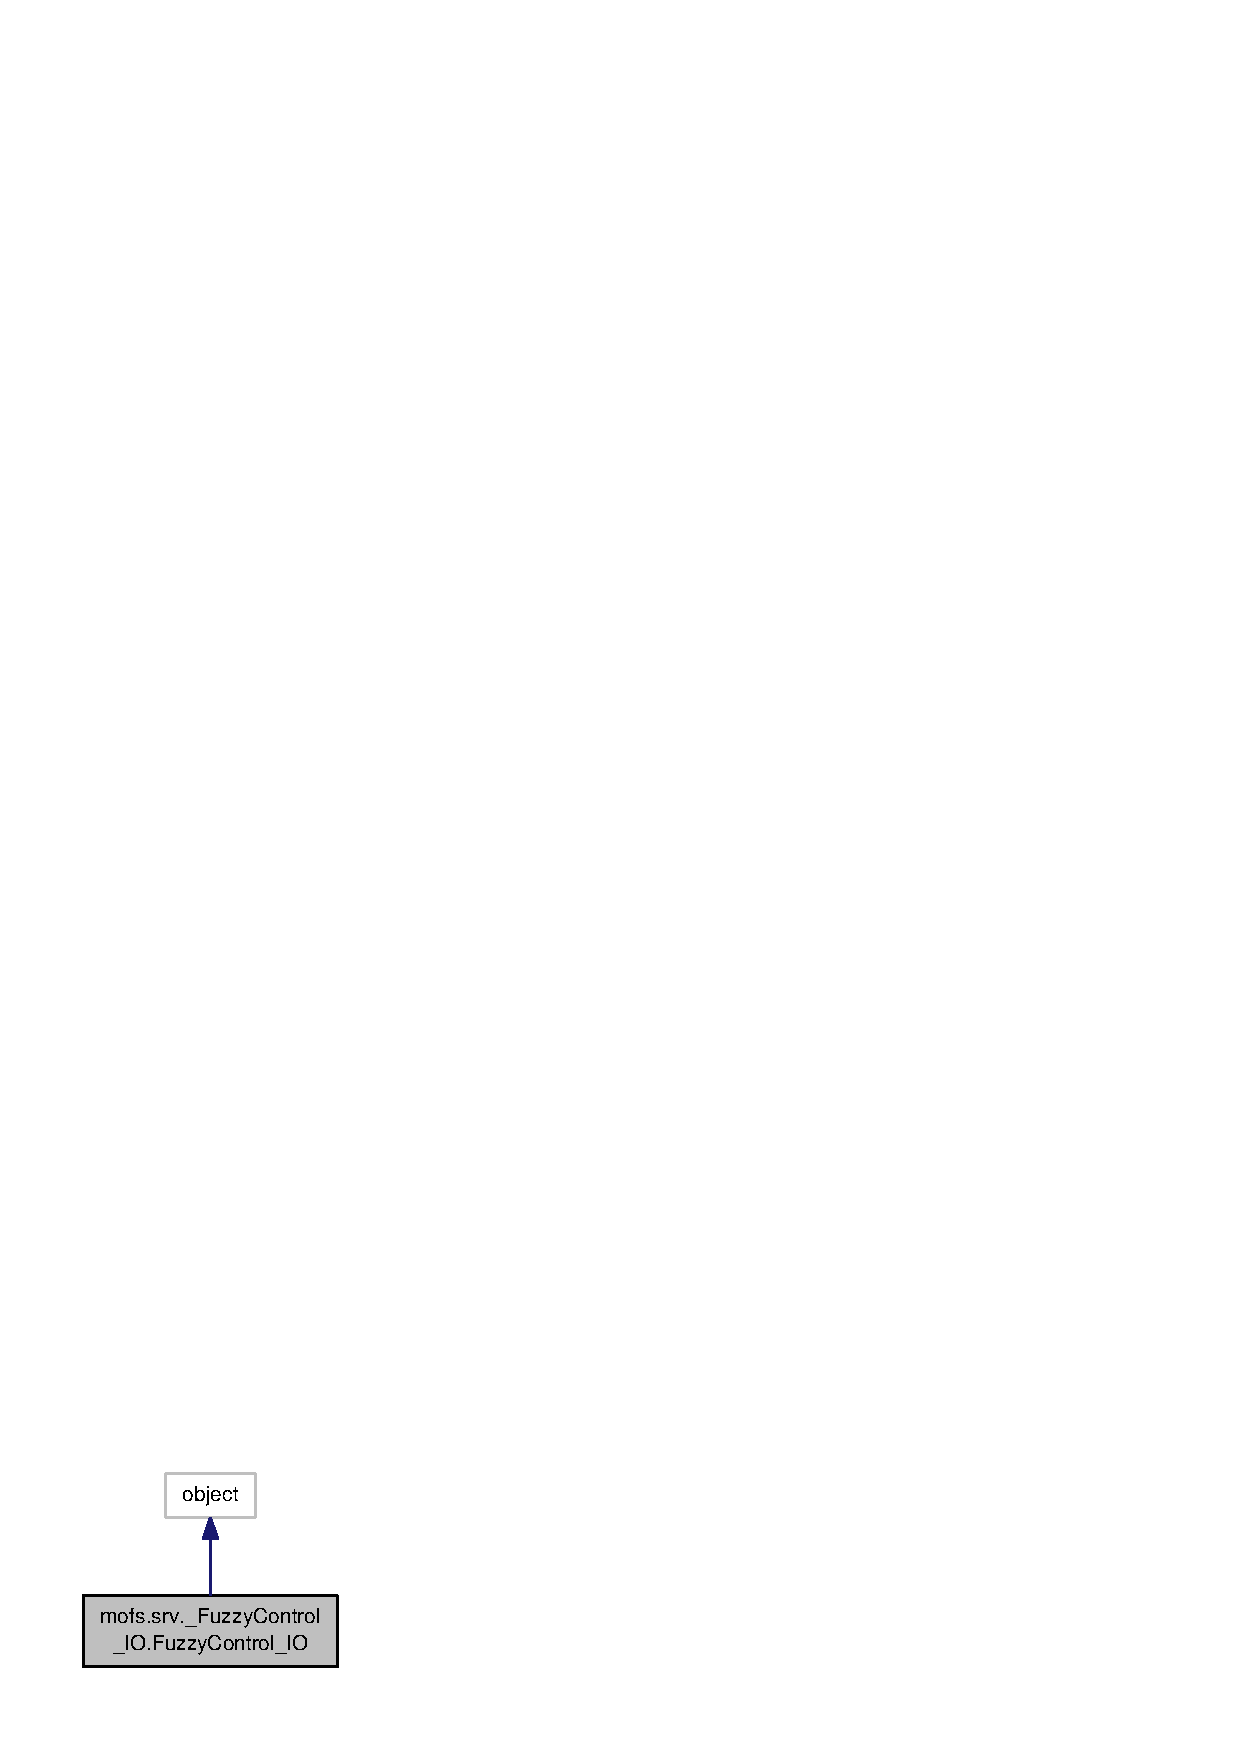
\includegraphics[width=166pt]{classmofs_1_1srv_1_1__FuzzyControl__IO_1_1FuzzyControl__IO__inherit__graph}
\end{center}
\end{figure}
\subsection*{Static Private Attributes}
\begin{DoxyCompactItemize}
\item 
string {\bf \-\_\-md5sum} = 'fba685fbdda96b6ff62d5238836ec32a'
\item 
{\bf \-\_\-request\-\_\-class} = {\bf Fuzzy\-Control\-\_\-\-I\-O\-Request}
\item 
{\bf \-\_\-response\-\_\-class} = {\bf Fuzzy\-Control\-\_\-\-I\-O\-Response}
\item 
string {\bf \-\_\-type} = 'mofs/{\bf Fuzzy\-Control\-\_\-\-I\-O}'
\end{DoxyCompactItemize}


\subsection{Detailed Description}


Definition at line 199 of file \-\_\-\-Fuzzy\-Control\-\_\-\-I\-O.\-py.



\subsection{Member Data Documentation}
\index{mofs\-::srv\-::\-\_\-\-Fuzzy\-Control\-\_\-\-I\-O\-::\-Fuzzy\-Control\-\_\-\-I\-O@{mofs\-::srv\-::\-\_\-\-Fuzzy\-Control\-\_\-\-I\-O\-::\-Fuzzy\-Control\-\_\-\-I\-O}!\-\_\-md5sum@{\-\_\-md5sum}}
\index{\-\_\-md5sum@{\-\_\-md5sum}!mofs::srv::_FuzzyControl_IO::FuzzyControl_IO@{mofs\-::srv\-::\-\_\-\-Fuzzy\-Control\-\_\-\-I\-O\-::\-Fuzzy\-Control\-\_\-\-I\-O}}
\subsubsection[{\-\_\-md5sum}]{\setlength{\rightskip}{0pt plus 5cm}string mofs.\-srv.\-\_\-\-Fuzzy\-Control\-\_\-\-I\-O.\-Fuzzy\-Control\-\_\-\-I\-O.\-\_\-md5sum = 'fba685fbdda96b6ff62d5238836ec32a'\hspace{0.3cm}{\ttfamily [static]}, {\ttfamily [private]}}\label{classmofs_1_1srv_1_1__FuzzyControl__IO_1_1FuzzyControl__IO_a77c38ca61a07f03a80f55fac2d4b8dac}


Definition at line 201 of file \-\_\-\-Fuzzy\-Control\-\_\-\-I\-O.\-py.

\index{mofs\-::srv\-::\-\_\-\-Fuzzy\-Control\-\_\-\-I\-O\-::\-Fuzzy\-Control\-\_\-\-I\-O@{mofs\-::srv\-::\-\_\-\-Fuzzy\-Control\-\_\-\-I\-O\-::\-Fuzzy\-Control\-\_\-\-I\-O}!\-\_\-request\-\_\-class@{\-\_\-request\-\_\-class}}
\index{\-\_\-request\-\_\-class@{\-\_\-request\-\_\-class}!mofs::srv::_FuzzyControl_IO::FuzzyControl_IO@{mofs\-::srv\-::\-\_\-\-Fuzzy\-Control\-\_\-\-I\-O\-::\-Fuzzy\-Control\-\_\-\-I\-O}}
\subsubsection[{\-\_\-request\-\_\-class}]{\setlength{\rightskip}{0pt plus 5cm}mofs.\-srv.\-\_\-\-Fuzzy\-Control\-\_\-\-I\-O.\-Fuzzy\-Control\-\_\-\-I\-O.\-\_\-request\-\_\-class = {\bf Fuzzy\-Control\-\_\-\-I\-O\-Request}\hspace{0.3cm}{\ttfamily [static]}, {\ttfamily [private]}}\label{classmofs_1_1srv_1_1__FuzzyControl__IO_1_1FuzzyControl__IO_a2bb072d15036297f44de74ece51165d9}


Definition at line 202 of file \-\_\-\-Fuzzy\-Control\-\_\-\-I\-O.\-py.

\index{mofs\-::srv\-::\-\_\-\-Fuzzy\-Control\-\_\-\-I\-O\-::\-Fuzzy\-Control\-\_\-\-I\-O@{mofs\-::srv\-::\-\_\-\-Fuzzy\-Control\-\_\-\-I\-O\-::\-Fuzzy\-Control\-\_\-\-I\-O}!\-\_\-response\-\_\-class@{\-\_\-response\-\_\-class}}
\index{\-\_\-response\-\_\-class@{\-\_\-response\-\_\-class}!mofs::srv::_FuzzyControl_IO::FuzzyControl_IO@{mofs\-::srv\-::\-\_\-\-Fuzzy\-Control\-\_\-\-I\-O\-::\-Fuzzy\-Control\-\_\-\-I\-O}}
\subsubsection[{\-\_\-response\-\_\-class}]{\setlength{\rightskip}{0pt plus 5cm}mofs.\-srv.\-\_\-\-Fuzzy\-Control\-\_\-\-I\-O.\-Fuzzy\-Control\-\_\-\-I\-O.\-\_\-response\-\_\-class = {\bf Fuzzy\-Control\-\_\-\-I\-O\-Response}\hspace{0.3cm}{\ttfamily [static]}, {\ttfamily [private]}}\label{classmofs_1_1srv_1_1__FuzzyControl__IO_1_1FuzzyControl__IO_a86c3ed67536ae8583dacff5c38567609}


Definition at line 203 of file \-\_\-\-Fuzzy\-Control\-\_\-\-I\-O.\-py.

\index{mofs\-::srv\-::\-\_\-\-Fuzzy\-Control\-\_\-\-I\-O\-::\-Fuzzy\-Control\-\_\-\-I\-O@{mofs\-::srv\-::\-\_\-\-Fuzzy\-Control\-\_\-\-I\-O\-::\-Fuzzy\-Control\-\_\-\-I\-O}!\-\_\-type@{\-\_\-type}}
\index{\-\_\-type@{\-\_\-type}!mofs::srv::_FuzzyControl_IO::FuzzyControl_IO@{mofs\-::srv\-::\-\_\-\-Fuzzy\-Control\-\_\-\-I\-O\-::\-Fuzzy\-Control\-\_\-\-I\-O}}
\subsubsection[{\-\_\-type}]{\setlength{\rightskip}{0pt plus 5cm}string mofs.\-srv.\-\_\-\-Fuzzy\-Control\-\_\-\-I\-O.\-Fuzzy\-Control\-\_\-\-I\-O.\-\_\-type = 'mofs/{\bf Fuzzy\-Control\-\_\-\-I\-O}'\hspace{0.3cm}{\ttfamily [static]}, {\ttfamily [private]}}\label{classmofs_1_1srv_1_1__FuzzyControl__IO_1_1FuzzyControl__IO_a87bac5f19336c3b57f0516c403064fce}


Definition at line 200 of file \-\_\-\-Fuzzy\-Control\-\_\-\-I\-O.\-py.



The documentation for this class was generated from the following file\-:\begin{DoxyCompactItemize}
\item 
{\bf \-\_\-\-Fuzzy\-Control\-\_\-\-I\-O.\-py}\end{DoxyCompactItemize}

\section{mofs\-:\-:Fuzzy\-Control\-\_\-\-I\-O Struct Reference}
\label{structmofs_1_1FuzzyControl__IO}\index{mofs\-::\-Fuzzy\-Control\-\_\-\-I\-O@{mofs\-::\-Fuzzy\-Control\-\_\-\-I\-O}}


{\ttfamily \#include $<$Fuzzy\-Control\-\_\-\-I\-O.\-h$>$}

\subsection*{Public Types}
\begin{DoxyCompactItemize}
\item 
typedef {\bf Fuzzy\-Control\-\_\-\-I\-O\-Request} {\bf Request}
\item 
typedef {\bf Request} {\bf Request\-Type}
\item 
typedef {\bf Fuzzy\-Control\-\_\-\-I\-O\-Response} {\bf Response}
\item 
typedef {\bf Response} {\bf Response\-Type}
\end{DoxyCompactItemize}
\subsection*{Public Attributes}
\begin{DoxyCompactItemize}
\item 
{\bf Request} {\bf request}
\item 
{\bf Response} {\bf response}
\end{DoxyCompactItemize}


\subsection{Detailed Description}


Definition at line 81 of file Fuzzy\-Control\-\_\-\-I\-O.\-h.



\subsection{Member Typedef Documentation}
\index{mofs\-::\-Fuzzy\-Control\-\_\-\-I\-O@{mofs\-::\-Fuzzy\-Control\-\_\-\-I\-O}!Request@{Request}}
\index{Request@{Request}!mofs::FuzzyControl_IO@{mofs\-::\-Fuzzy\-Control\-\_\-\-I\-O}}
\subsubsection[{Request}]{\setlength{\rightskip}{0pt plus 5cm}typedef {\bf Fuzzy\-Control\-\_\-\-I\-O\-Request} {\bf mofs\-::\-Fuzzy\-Control\-\_\-\-I\-O\-::\-Request}}\label{structmofs_1_1FuzzyControl__IO_a2a71684b8b3b362786c0c7cb3ff35613}


Definition at line 84 of file Fuzzy\-Control\-\_\-\-I\-O.\-h.

\index{mofs\-::\-Fuzzy\-Control\-\_\-\-I\-O@{mofs\-::\-Fuzzy\-Control\-\_\-\-I\-O}!Request\-Type@{Request\-Type}}
\index{Request\-Type@{Request\-Type}!mofs::FuzzyControl_IO@{mofs\-::\-Fuzzy\-Control\-\_\-\-I\-O}}
\subsubsection[{Request\-Type}]{\setlength{\rightskip}{0pt plus 5cm}typedef {\bf Request} {\bf mofs\-::\-Fuzzy\-Control\-\_\-\-I\-O\-::\-Request\-Type}}\label{structmofs_1_1FuzzyControl__IO_a60ea85600e477218068d982a36f40882}


Definition at line 89 of file Fuzzy\-Control\-\_\-\-I\-O.\-h.

\index{mofs\-::\-Fuzzy\-Control\-\_\-\-I\-O@{mofs\-::\-Fuzzy\-Control\-\_\-\-I\-O}!Response@{Response}}
\index{Response@{Response}!mofs::FuzzyControl_IO@{mofs\-::\-Fuzzy\-Control\-\_\-\-I\-O}}
\subsubsection[{Response}]{\setlength{\rightskip}{0pt plus 5cm}typedef {\bf Fuzzy\-Control\-\_\-\-I\-O\-Response} {\bf mofs\-::\-Fuzzy\-Control\-\_\-\-I\-O\-::\-Response}}\label{structmofs_1_1FuzzyControl__IO_a679e83978a022d15b0397aea40603565}


Definition at line 85 of file Fuzzy\-Control\-\_\-\-I\-O.\-h.

\index{mofs\-::\-Fuzzy\-Control\-\_\-\-I\-O@{mofs\-::\-Fuzzy\-Control\-\_\-\-I\-O}!Response\-Type@{Response\-Type}}
\index{Response\-Type@{Response\-Type}!mofs::FuzzyControl_IO@{mofs\-::\-Fuzzy\-Control\-\_\-\-I\-O}}
\subsubsection[{Response\-Type}]{\setlength{\rightskip}{0pt plus 5cm}typedef {\bf Response} {\bf mofs\-::\-Fuzzy\-Control\-\_\-\-I\-O\-::\-Response\-Type}}\label{structmofs_1_1FuzzyControl__IO_aeaea778dd837bd75c31dcd7d7bb7185d}


Definition at line 90 of file Fuzzy\-Control\-\_\-\-I\-O.\-h.



\subsection{Member Data Documentation}
\index{mofs\-::\-Fuzzy\-Control\-\_\-\-I\-O@{mofs\-::\-Fuzzy\-Control\-\_\-\-I\-O}!request@{request}}
\index{request@{request}!mofs::FuzzyControl_IO@{mofs\-::\-Fuzzy\-Control\-\_\-\-I\-O}}
\subsubsection[{request}]{\setlength{\rightskip}{0pt plus 5cm}{\bf Request} mofs\-::\-Fuzzy\-Control\-\_\-\-I\-O\-::request}\label{structmofs_1_1FuzzyControl__IO_a42ad357ca0c759a9e1e9abb501f38586}


Definition at line 86 of file Fuzzy\-Control\-\_\-\-I\-O.\-h.

\index{mofs\-::\-Fuzzy\-Control\-\_\-\-I\-O@{mofs\-::\-Fuzzy\-Control\-\_\-\-I\-O}!response@{response}}
\index{response@{response}!mofs::FuzzyControl_IO@{mofs\-::\-Fuzzy\-Control\-\_\-\-I\-O}}
\subsubsection[{response}]{\setlength{\rightskip}{0pt plus 5cm}{\bf Response} mofs\-::\-Fuzzy\-Control\-\_\-\-I\-O\-::response}\label{structmofs_1_1FuzzyControl__IO_aff372393f399a7a6ea23ac813fb36462}


Definition at line 87 of file Fuzzy\-Control\-\_\-\-I\-O.\-h.



The documentation for this struct was generated from the following file\-:\begin{DoxyCompactItemize}
\item 
{\bf Fuzzy\-Control\-\_\-\-I\-O.\-h}\end{DoxyCompactItemize}

\section{mofs.\-srv.\-\_\-\-Fuzzy\-Control\-\_\-\-I\-O.\-Fuzzy\-Control\-\_\-\-I\-O\-Request Class Reference}
\label{classmofs_1_1srv_1_1__FuzzyControl__IO_1_1FuzzyControl__IORequest}\index{mofs.\-srv.\-\_\-\-Fuzzy\-Control\-\_\-\-I\-O.\-Fuzzy\-Control\-\_\-\-I\-O\-Request@{mofs.\-srv.\-\_\-\-Fuzzy\-Control\-\_\-\-I\-O.\-Fuzzy\-Control\-\_\-\-I\-O\-Request}}


Inheritance diagram for mofs.\-srv.\-\_\-\-Fuzzy\-Control\-\_\-\-I\-O.\-Fuzzy\-Control\-\_\-\-I\-O\-Request\-:\nopagebreak
\begin{figure}[H]
\begin{center}
\leavevmode
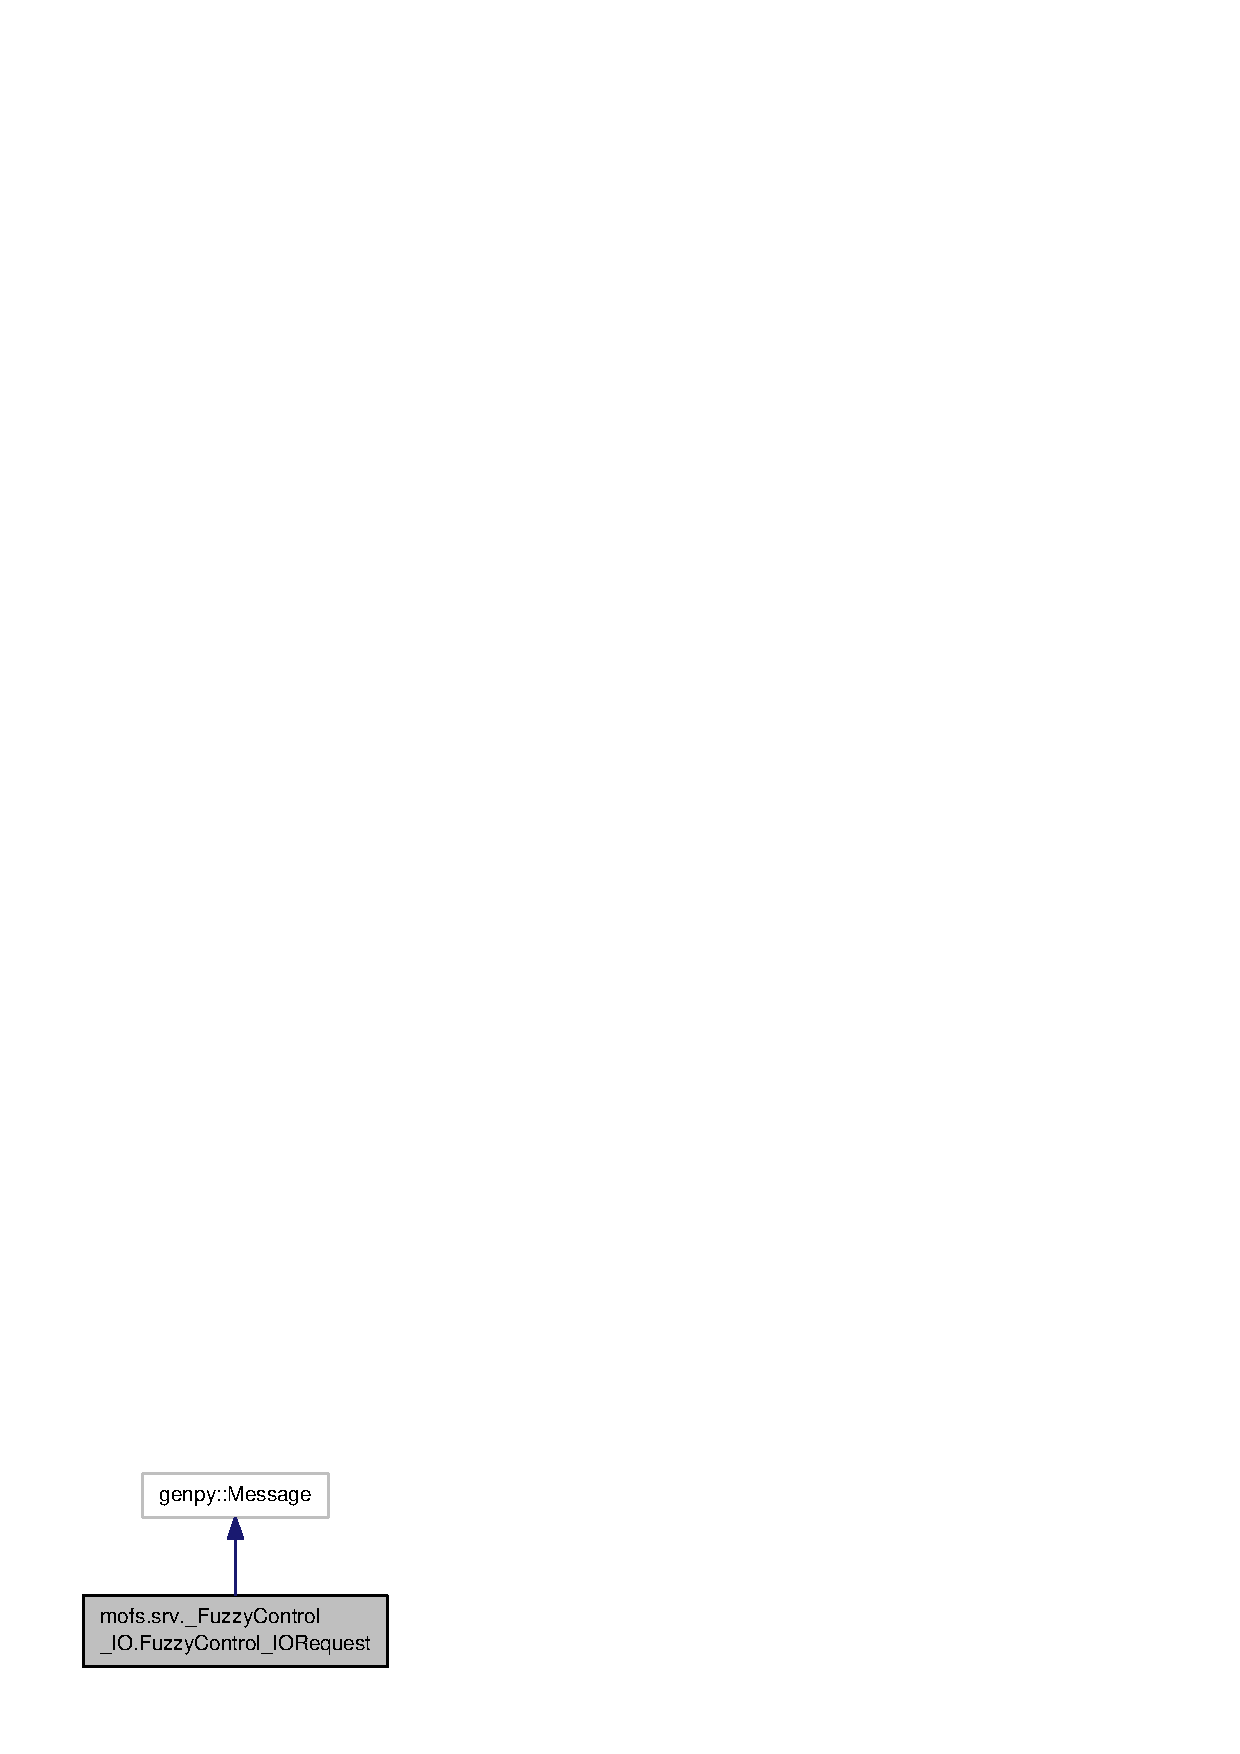
\includegraphics[width=190pt]{classmofs_1_1srv_1_1__FuzzyControl__IO_1_1FuzzyControl__IORequest__inherit__graph}
\end{center}
\end{figure}
\subsection*{Public Member Functions}
\begin{DoxyCompactItemize}
\item 
def {\bf \-\_\-\-\_\-init\-\_\-\-\_\-}
\item 
def {\bf deserialize}
\item 
def {\bf deserialize\-\_\-numpy}
\item 
def {\bf serialize}
\item 
def {\bf serialize\-\_\-numpy}
\end{DoxyCompactItemize}
\subsection*{Public Attributes}
\begin{DoxyCompactItemize}
\item 
{\bf inputs}
\end{DoxyCompactItemize}
\subsection*{Private Member Functions}
\begin{DoxyCompactItemize}
\item 
def {\bf \-\_\-get\-\_\-types}
\end{DoxyCompactItemize}
\subsection*{Static Private Attributes}
\begin{DoxyCompactItemize}
\item 
list {\bf \-\_\-\-\_\-slots\-\_\-\-\_\-} = ['{\bf inputs}']
\item 
string {\bf \-\_\-full\-\_\-text}
\item 
{\bf \-\_\-has\-\_\-header} = False
\item 
string {\bf \-\_\-md5sum} = \char`\"{}ea0b038bccdff67bc1751623cde4aed3\char`\"{}
\item 
list {\bf \-\_\-slot\-\_\-types} = ['float32[3]']
\item 
string {\bf \-\_\-type} = \char`\"{}mofs/{\bf Fuzzy\-Control\-\_\-\-I\-O\-Request}\char`\"{}
\end{DoxyCompactItemize}


\subsection{Detailed Description}


Definition at line 8 of file \-\_\-\-Fuzzy\-Control\-\_\-\-I\-O.\-py.



\subsection{Constructor \& Destructor Documentation}
\index{mofs\-::srv\-::\-\_\-\-Fuzzy\-Control\-\_\-\-I\-O\-::\-Fuzzy\-Control\-\_\-\-I\-O\-Request@{mofs\-::srv\-::\-\_\-\-Fuzzy\-Control\-\_\-\-I\-O\-::\-Fuzzy\-Control\-\_\-\-I\-O\-Request}!\-\_\-\-\_\-init\-\_\-\-\_\-@{\-\_\-\-\_\-init\-\_\-\-\_\-}}
\index{\-\_\-\-\_\-init\-\_\-\-\_\-@{\-\_\-\-\_\-init\-\_\-\-\_\-}!mofs::srv::_FuzzyControl_IO::FuzzyControl_IORequest@{mofs\-::srv\-::\-\_\-\-Fuzzy\-Control\-\_\-\-I\-O\-::\-Fuzzy\-Control\-\_\-\-I\-O\-Request}}
\subsubsection[{\-\_\-\-\_\-init\-\_\-\-\_\-}]{\setlength{\rightskip}{0pt plus 5cm}def mofs.\-srv.\-\_\-\-Fuzzy\-Control\-\_\-\-I\-O.\-Fuzzy\-Control\-\_\-\-I\-O\-Request.\-\_\-\-\_\-init\-\_\-\-\_\- (
\begin{DoxyParamCaption}
\item[{}]{self, }
\item[{}]{args, }
\item[{}]{kwds}
\end{DoxyParamCaption}
)}\label{classmofs_1_1srv_1_1__FuzzyControl__IO_1_1FuzzyControl__IORequest_a4d08917ae21c884ede3c0f5f9944c221}
\begin{DoxyVerb}Constructor. Any message fields that are implicitly/explicitly
set to None will be assigned a default value. The recommend
use is keyword arguments as this is more robust to future message
changes.  You cannot mix in-order arguments and keyword arguments.

The available fields are:
   inputs

:param args: complete set of field values, in .msg order
:param kwds: use keyword arguments corresponding to message field names
to set specific fields.
\end{DoxyVerb}
 

Definition at line 19 of file \-\_\-\-Fuzzy\-Control\-\_\-\-I\-O.\-py.



\subsection{Member Function Documentation}
\index{mofs\-::srv\-::\-\_\-\-Fuzzy\-Control\-\_\-\-I\-O\-::\-Fuzzy\-Control\-\_\-\-I\-O\-Request@{mofs\-::srv\-::\-\_\-\-Fuzzy\-Control\-\_\-\-I\-O\-::\-Fuzzy\-Control\-\_\-\-I\-O\-Request}!\-\_\-get\-\_\-types@{\-\_\-get\-\_\-types}}
\index{\-\_\-get\-\_\-types@{\-\_\-get\-\_\-types}!mofs::srv::_FuzzyControl_IO::FuzzyControl_IORequest@{mofs\-::srv\-::\-\_\-\-Fuzzy\-Control\-\_\-\-I\-O\-::\-Fuzzy\-Control\-\_\-\-I\-O\-Request}}
\subsubsection[{\-\_\-get\-\_\-types}]{\setlength{\rightskip}{0pt plus 5cm}def mofs.\-srv.\-\_\-\-Fuzzy\-Control\-\_\-\-I\-O.\-Fuzzy\-Control\-\_\-\-I\-O\-Request.\-\_\-get\-\_\-types (
\begin{DoxyParamCaption}
\item[{}]{self}
\end{DoxyParamCaption}
)\hspace{0.3cm}{\ttfamily [private]}}\label{classmofs_1_1srv_1_1__FuzzyControl__IO_1_1FuzzyControl__IORequest_a17e450daefdd6a2c014461f8a22894fe}
\begin{DoxyVerb}internal API method
\end{DoxyVerb}
 

Definition at line 41 of file \-\_\-\-Fuzzy\-Control\-\_\-\-I\-O.\-py.

\index{mofs\-::srv\-::\-\_\-\-Fuzzy\-Control\-\_\-\-I\-O\-::\-Fuzzy\-Control\-\_\-\-I\-O\-Request@{mofs\-::srv\-::\-\_\-\-Fuzzy\-Control\-\_\-\-I\-O\-::\-Fuzzy\-Control\-\_\-\-I\-O\-Request}!deserialize@{deserialize}}
\index{deserialize@{deserialize}!mofs::srv::_FuzzyControl_IO::FuzzyControl_IORequest@{mofs\-::srv\-::\-\_\-\-Fuzzy\-Control\-\_\-\-I\-O\-::\-Fuzzy\-Control\-\_\-\-I\-O\-Request}}
\subsubsection[{deserialize}]{\setlength{\rightskip}{0pt plus 5cm}def mofs.\-srv.\-\_\-\-Fuzzy\-Control\-\_\-\-I\-O.\-Fuzzy\-Control\-\_\-\-I\-O\-Request.\-deserialize (
\begin{DoxyParamCaption}
\item[{}]{self, }
\item[{}]{str}
\end{DoxyParamCaption}
)}\label{classmofs_1_1srv_1_1__FuzzyControl__IO_1_1FuzzyControl__IORequest_add978ec83b456fc30e25d6dca2f34562}
\begin{DoxyVerb}unpack serialized message in str into this message instance
:param str: byte array of serialized message, ``str``
\end{DoxyVerb}
 

Definition at line 57 of file \-\_\-\-Fuzzy\-Control\-\_\-\-I\-O.\-py.

\index{mofs\-::srv\-::\-\_\-\-Fuzzy\-Control\-\_\-\-I\-O\-::\-Fuzzy\-Control\-\_\-\-I\-O\-Request@{mofs\-::srv\-::\-\_\-\-Fuzzy\-Control\-\_\-\-I\-O\-::\-Fuzzy\-Control\-\_\-\-I\-O\-Request}!deserialize\-\_\-numpy@{deserialize\-\_\-numpy}}
\index{deserialize\-\_\-numpy@{deserialize\-\_\-numpy}!mofs::srv::_FuzzyControl_IO::FuzzyControl_IORequest@{mofs\-::srv\-::\-\_\-\-Fuzzy\-Control\-\_\-\-I\-O\-::\-Fuzzy\-Control\-\_\-\-I\-O\-Request}}
\subsubsection[{deserialize\-\_\-numpy}]{\setlength{\rightskip}{0pt plus 5cm}def mofs.\-srv.\-\_\-\-Fuzzy\-Control\-\_\-\-I\-O.\-Fuzzy\-Control\-\_\-\-I\-O\-Request.\-deserialize\-\_\-numpy (
\begin{DoxyParamCaption}
\item[{}]{self, }
\item[{}]{str, }
\item[{}]{numpy}
\end{DoxyParamCaption}
)}\label{classmofs_1_1srv_1_1__FuzzyControl__IO_1_1FuzzyControl__IORequest_afb5a94e0491acb947ac05982f746702f}
\begin{DoxyVerb}unpack serialized message in str into this message instance using numpy for array types
:param str: byte array of serialized message, ``str``
:param numpy: numpy python module
\end{DoxyVerb}
 

Definition at line 83 of file \-\_\-\-Fuzzy\-Control\-\_\-\-I\-O.\-py.

\index{mofs\-::srv\-::\-\_\-\-Fuzzy\-Control\-\_\-\-I\-O\-::\-Fuzzy\-Control\-\_\-\-I\-O\-Request@{mofs\-::srv\-::\-\_\-\-Fuzzy\-Control\-\_\-\-I\-O\-::\-Fuzzy\-Control\-\_\-\-I\-O\-Request}!serialize@{serialize}}
\index{serialize@{serialize}!mofs::srv::_FuzzyControl_IO::FuzzyControl_IORequest@{mofs\-::srv\-::\-\_\-\-Fuzzy\-Control\-\_\-\-I\-O\-::\-Fuzzy\-Control\-\_\-\-I\-O\-Request}}
\subsubsection[{serialize}]{\setlength{\rightskip}{0pt plus 5cm}def mofs.\-srv.\-\_\-\-Fuzzy\-Control\-\_\-\-I\-O.\-Fuzzy\-Control\-\_\-\-I\-O\-Request.\-serialize (
\begin{DoxyParamCaption}
\item[{}]{self, }
\item[{}]{buff}
\end{DoxyParamCaption}
)}\label{classmofs_1_1srv_1_1__FuzzyControl__IO_1_1FuzzyControl__IORequest_a6eb66ccfb93e3473a073ff20ab80eb2e}
\begin{DoxyVerb}serialize message into buffer
:param buff: buffer, ``StringIO``
\end{DoxyVerb}
 

Definition at line 47 of file \-\_\-\-Fuzzy\-Control\-\_\-\-I\-O.\-py.

\index{mofs\-::srv\-::\-\_\-\-Fuzzy\-Control\-\_\-\-I\-O\-::\-Fuzzy\-Control\-\_\-\-I\-O\-Request@{mofs\-::srv\-::\-\_\-\-Fuzzy\-Control\-\_\-\-I\-O\-::\-Fuzzy\-Control\-\_\-\-I\-O\-Request}!serialize\-\_\-numpy@{serialize\-\_\-numpy}}
\index{serialize\-\_\-numpy@{serialize\-\_\-numpy}!mofs::srv::_FuzzyControl_IO::FuzzyControl_IORequest@{mofs\-::srv\-::\-\_\-\-Fuzzy\-Control\-\_\-\-I\-O\-::\-Fuzzy\-Control\-\_\-\-I\-O\-Request}}
\subsubsection[{serialize\-\_\-numpy}]{\setlength{\rightskip}{0pt plus 5cm}def mofs.\-srv.\-\_\-\-Fuzzy\-Control\-\_\-\-I\-O.\-Fuzzy\-Control\-\_\-\-I\-O\-Request.\-serialize\-\_\-numpy (
\begin{DoxyParamCaption}
\item[{}]{self, }
\item[{}]{buff, }
\item[{}]{numpy}
\end{DoxyParamCaption}
)}\label{classmofs_1_1srv_1_1__FuzzyControl__IO_1_1FuzzyControl__IORequest_a8ce28620da4fb21c0ad599fcbc493a97}
\begin{DoxyVerb}serialize message with numpy array types into buffer
:param buff: buffer, ``StringIO``
:param numpy: numpy python module
\end{DoxyVerb}
 

Definition at line 72 of file \-\_\-\-Fuzzy\-Control\-\_\-\-I\-O.\-py.



\subsection{Member Data Documentation}
\index{mofs\-::srv\-::\-\_\-\-Fuzzy\-Control\-\_\-\-I\-O\-::\-Fuzzy\-Control\-\_\-\-I\-O\-Request@{mofs\-::srv\-::\-\_\-\-Fuzzy\-Control\-\_\-\-I\-O\-::\-Fuzzy\-Control\-\_\-\-I\-O\-Request}!\-\_\-\-\_\-slots\-\_\-\-\_\-@{\-\_\-\-\_\-slots\-\_\-\-\_\-}}
\index{\-\_\-\-\_\-slots\-\_\-\-\_\-@{\-\_\-\-\_\-slots\-\_\-\-\_\-}!mofs::srv::_FuzzyControl_IO::FuzzyControl_IORequest@{mofs\-::srv\-::\-\_\-\-Fuzzy\-Control\-\_\-\-I\-O\-::\-Fuzzy\-Control\-\_\-\-I\-O\-Request}}
\subsubsection[{\-\_\-\-\_\-slots\-\_\-\-\_\-}]{\setlength{\rightskip}{0pt plus 5cm}list mofs.\-srv.\-\_\-\-Fuzzy\-Control\-\_\-\-I\-O.\-Fuzzy\-Control\-\_\-\-I\-O\-Request.\-\_\-\-\_\-slots\-\_\-\-\_\- = ['{\bf inputs}']\hspace{0.3cm}{\ttfamily [static]}, {\ttfamily [private]}}\label{classmofs_1_1srv_1_1__FuzzyControl__IO_1_1FuzzyControl__IORequest_ab925438ddef71d55b03d2f94380a9a28}


Definition at line 16 of file \-\_\-\-Fuzzy\-Control\-\_\-\-I\-O.\-py.

\index{mofs\-::srv\-::\-\_\-\-Fuzzy\-Control\-\_\-\-I\-O\-::\-Fuzzy\-Control\-\_\-\-I\-O\-Request@{mofs\-::srv\-::\-\_\-\-Fuzzy\-Control\-\_\-\-I\-O\-::\-Fuzzy\-Control\-\_\-\-I\-O\-Request}!\-\_\-full\-\_\-text@{\-\_\-full\-\_\-text}}
\index{\-\_\-full\-\_\-text@{\-\_\-full\-\_\-text}!mofs::srv::_FuzzyControl_IO::FuzzyControl_IORequest@{mofs\-::srv\-::\-\_\-\-Fuzzy\-Control\-\_\-\-I\-O\-::\-Fuzzy\-Control\-\_\-\-I\-O\-Request}}
\subsubsection[{\-\_\-full\-\_\-text}]{\setlength{\rightskip}{0pt plus 5cm}string mofs.\-srv.\-\_\-\-Fuzzy\-Control\-\_\-\-I\-O.\-Fuzzy\-Control\-\_\-\-I\-O\-Request.\-\_\-full\-\_\-text\hspace{0.3cm}{\ttfamily [static]}, {\ttfamily [private]}}\label{classmofs_1_1srv_1_1__FuzzyControl__IO_1_1FuzzyControl__IORequest_a6933818df2b2ac5be1f2a7656bf146a4}
{\bfseries Initial value\-:}
\begin{DoxyCode}
1 = \textcolor{stringliteral}{"""}
2 \textcolor{stringliteral}{float32[3] inputs}
3 \textcolor{stringliteral}{}
4 \textcolor{stringliteral}{"""}
\end{DoxyCode}


Definition at line 12 of file \-\_\-\-Fuzzy\-Control\-\_\-\-I\-O.\-py.

\index{mofs\-::srv\-::\-\_\-\-Fuzzy\-Control\-\_\-\-I\-O\-::\-Fuzzy\-Control\-\_\-\-I\-O\-Request@{mofs\-::srv\-::\-\_\-\-Fuzzy\-Control\-\_\-\-I\-O\-::\-Fuzzy\-Control\-\_\-\-I\-O\-Request}!\-\_\-has\-\_\-header@{\-\_\-has\-\_\-header}}
\index{\-\_\-has\-\_\-header@{\-\_\-has\-\_\-header}!mofs::srv::_FuzzyControl_IO::FuzzyControl_IORequest@{mofs\-::srv\-::\-\_\-\-Fuzzy\-Control\-\_\-\-I\-O\-::\-Fuzzy\-Control\-\_\-\-I\-O\-Request}}
\subsubsection[{\-\_\-has\-\_\-header}]{\setlength{\rightskip}{0pt plus 5cm}mofs.\-srv.\-\_\-\-Fuzzy\-Control\-\_\-\-I\-O.\-Fuzzy\-Control\-\_\-\-I\-O\-Request.\-\_\-has\-\_\-header = False\hspace{0.3cm}{\ttfamily [static]}, {\ttfamily [private]}}\label{classmofs_1_1srv_1_1__FuzzyControl__IO_1_1FuzzyControl__IORequest_a4fb789d93d7b53a5da576ea5b31b3cb2}


Definition at line 11 of file \-\_\-\-Fuzzy\-Control\-\_\-\-I\-O.\-py.

\index{mofs\-::srv\-::\-\_\-\-Fuzzy\-Control\-\_\-\-I\-O\-::\-Fuzzy\-Control\-\_\-\-I\-O\-Request@{mofs\-::srv\-::\-\_\-\-Fuzzy\-Control\-\_\-\-I\-O\-::\-Fuzzy\-Control\-\_\-\-I\-O\-Request}!\-\_\-md5sum@{\-\_\-md5sum}}
\index{\-\_\-md5sum@{\-\_\-md5sum}!mofs::srv::_FuzzyControl_IO::FuzzyControl_IORequest@{mofs\-::srv\-::\-\_\-\-Fuzzy\-Control\-\_\-\-I\-O\-::\-Fuzzy\-Control\-\_\-\-I\-O\-Request}}
\subsubsection[{\-\_\-md5sum}]{\setlength{\rightskip}{0pt plus 5cm}string mofs.\-srv.\-\_\-\-Fuzzy\-Control\-\_\-\-I\-O.\-Fuzzy\-Control\-\_\-\-I\-O\-Request.\-\_\-md5sum = \char`\"{}ea0b038bccdff67bc1751623cde4aed3\char`\"{}\hspace{0.3cm}{\ttfamily [static]}, {\ttfamily [private]}}\label{classmofs_1_1srv_1_1__FuzzyControl__IO_1_1FuzzyControl__IORequest_a19043db416ac45722eea4a7cd8eebe5f}


Definition at line 9 of file \-\_\-\-Fuzzy\-Control\-\_\-\-I\-O.\-py.

\index{mofs\-::srv\-::\-\_\-\-Fuzzy\-Control\-\_\-\-I\-O\-::\-Fuzzy\-Control\-\_\-\-I\-O\-Request@{mofs\-::srv\-::\-\_\-\-Fuzzy\-Control\-\_\-\-I\-O\-::\-Fuzzy\-Control\-\_\-\-I\-O\-Request}!\-\_\-slot\-\_\-types@{\-\_\-slot\-\_\-types}}
\index{\-\_\-slot\-\_\-types@{\-\_\-slot\-\_\-types}!mofs::srv::_FuzzyControl_IO::FuzzyControl_IORequest@{mofs\-::srv\-::\-\_\-\-Fuzzy\-Control\-\_\-\-I\-O\-::\-Fuzzy\-Control\-\_\-\-I\-O\-Request}}
\subsubsection[{\-\_\-slot\-\_\-types}]{\setlength{\rightskip}{0pt plus 5cm}list mofs.\-srv.\-\_\-\-Fuzzy\-Control\-\_\-\-I\-O.\-Fuzzy\-Control\-\_\-\-I\-O\-Request.\-\_\-slot\-\_\-types = ['float32[3]']\hspace{0.3cm}{\ttfamily [static]}, {\ttfamily [private]}}\label{classmofs_1_1srv_1_1__FuzzyControl__IO_1_1FuzzyControl__IORequest_ad0cce3b41c3ee5f0a04b682a1d1494ed}


Definition at line 17 of file \-\_\-\-Fuzzy\-Control\-\_\-\-I\-O.\-py.

\index{mofs\-::srv\-::\-\_\-\-Fuzzy\-Control\-\_\-\-I\-O\-::\-Fuzzy\-Control\-\_\-\-I\-O\-Request@{mofs\-::srv\-::\-\_\-\-Fuzzy\-Control\-\_\-\-I\-O\-::\-Fuzzy\-Control\-\_\-\-I\-O\-Request}!\-\_\-type@{\-\_\-type}}
\index{\-\_\-type@{\-\_\-type}!mofs::srv::_FuzzyControl_IO::FuzzyControl_IORequest@{mofs\-::srv\-::\-\_\-\-Fuzzy\-Control\-\_\-\-I\-O\-::\-Fuzzy\-Control\-\_\-\-I\-O\-Request}}
\subsubsection[{\-\_\-type}]{\setlength{\rightskip}{0pt plus 5cm}string mofs.\-srv.\-\_\-\-Fuzzy\-Control\-\_\-\-I\-O.\-Fuzzy\-Control\-\_\-\-I\-O\-Request.\-\_\-type = \char`\"{}mofs/{\bf Fuzzy\-Control\-\_\-\-I\-O\-Request}\char`\"{}\hspace{0.3cm}{\ttfamily [static]}, {\ttfamily [private]}}\label{classmofs_1_1srv_1_1__FuzzyControl__IO_1_1FuzzyControl__IORequest_ad3044018c91643173e446fd744917bce}


Definition at line 10 of file \-\_\-\-Fuzzy\-Control\-\_\-\-I\-O.\-py.

\index{mofs\-::srv\-::\-\_\-\-Fuzzy\-Control\-\_\-\-I\-O\-::\-Fuzzy\-Control\-\_\-\-I\-O\-Request@{mofs\-::srv\-::\-\_\-\-Fuzzy\-Control\-\_\-\-I\-O\-::\-Fuzzy\-Control\-\_\-\-I\-O\-Request}!inputs@{inputs}}
\index{inputs@{inputs}!mofs::srv::_FuzzyControl_IO::FuzzyControl_IORequest@{mofs\-::srv\-::\-\_\-\-Fuzzy\-Control\-\_\-\-I\-O\-::\-Fuzzy\-Control\-\_\-\-I\-O\-Request}}
\subsubsection[{inputs}]{\setlength{\rightskip}{0pt plus 5cm}mofs.\-srv.\-\_\-\-Fuzzy\-Control\-\_\-\-I\-O.\-Fuzzy\-Control\-\_\-\-I\-O\-Request.\-inputs}\label{classmofs_1_1srv_1_1__FuzzyControl__IO_1_1FuzzyControl__IORequest_a158fae99f479ce7650bf542b61749d89}


Definition at line 37 of file \-\_\-\-Fuzzy\-Control\-\_\-\-I\-O.\-py.



The documentation for this class was generated from the following file\-:\begin{DoxyCompactItemize}
\item 
{\bf \-\_\-\-Fuzzy\-Control\-\_\-\-I\-O.\-py}\end{DoxyCompactItemize}

\section{mofs\-:\-:Fuzzy\-Control\-\_\-\-I\-O\-Request\-\_\-$<$ Container\-Allocator $>$ Struct Template Reference}
\label{structmofs_1_1FuzzyControl__IORequest__}\index{mofs\-::\-Fuzzy\-Control\-\_\-\-I\-O\-Request\-\_\-$<$ Container\-Allocator $>$@{mofs\-::\-Fuzzy\-Control\-\_\-\-I\-O\-Request\-\_\-$<$ Container\-Allocator $>$}}


{\ttfamily \#include $<$Fuzzy\-Control\-\_\-\-I\-O.\-h$>$}

\subsection*{Public Types}
\begin{DoxyCompactItemize}
\item 
typedef boost\-::array$<$ float, 3 $>$ {\bf \-\_\-inputs\-\_\-type}
\item 
typedef boost\-::shared\-\_\-ptr\\*
$<$ \-::{\bf mofs\-::\-Fuzzy\-Control\-\_\-\-I\-O\-Request\-\_\-}\\*
$<$ Container\-Allocator $>$ const  $>$ {\bf Const\-Ptr}
\item 
typedef boost\-::shared\-\_\-ptr\\*
$<$ \-::{\bf mofs\-::\-Fuzzy\-Control\-\_\-\-I\-O\-Request\-\_\-}\\*
$<$ Container\-Allocator $>$ $>$ {\bf Ptr}
\item 
typedef \\*
{\bf Fuzzy\-Control\-\_\-\-I\-O\-Request\-\_\-}\\*
$<$ Container\-Allocator $>$ {\bf Type}
\end{DoxyCompactItemize}
\subsection*{Public Member Functions}
\begin{DoxyCompactItemize}
\item 
{\bf Fuzzy\-Control\-\_\-\-I\-O\-Request\-\_\-} ()
\item 
{\bf Fuzzy\-Control\-\_\-\-I\-O\-Request\-\_\-} (const Container\-Allocator \&\-\_\-alloc)
\end{DoxyCompactItemize}
\subsection*{Public Attributes}
\begin{DoxyCompactItemize}
\item 
boost\-::shared\-\_\-ptr$<$ std\-::map\\*
$<$ std\-::string, std\-::string $>$ $>$ {\bf \-\_\-\-\_\-connection\-\_\-header}
\item 
boost\-::array$<$ float, 3 $>$ {\bf inputs}
\end{DoxyCompactItemize}


\subsection{Detailed Description}
\subsubsection*{template$<$class Container\-Allocator$>$struct mofs\-::\-Fuzzy\-Control\-\_\-\-I\-O\-Request\-\_\-$<$ Container\-Allocator $>$}



Definition at line 25 of file Fuzzy\-Control\-\_\-\-I\-O.\-h.



\subsection{Member Typedef Documentation}
\index{mofs\-::\-Fuzzy\-Control\-\_\-\-I\-O\-Request\-\_\-@{mofs\-::\-Fuzzy\-Control\-\_\-\-I\-O\-Request\-\_\-}!\-\_\-inputs\-\_\-type@{\-\_\-inputs\-\_\-type}}
\index{\-\_\-inputs\-\_\-type@{\-\_\-inputs\-\_\-type}!mofs::FuzzyControl_IORequest_@{mofs\-::\-Fuzzy\-Control\-\_\-\-I\-O\-Request\-\_\-}}
\subsubsection[{\-\_\-inputs\-\_\-type}]{\setlength{\rightskip}{0pt plus 5cm}template$<$class Container\-Allocator $>$ typedef boost\-::array$<$float, 3$>$ {\bf mofs\-::\-Fuzzy\-Control\-\_\-\-I\-O\-Request\-\_\-}$<$ Container\-Allocator $>$\-::{\bf \-\_\-inputs\-\_\-type}}\label{structmofs_1_1FuzzyControl__IORequest___a8bf3c09eab0aa2be3371511ba6d5237e}


Definition at line 40 of file Fuzzy\-Control\-\_\-\-I\-O.\-h.

\index{mofs\-::\-Fuzzy\-Control\-\_\-\-I\-O\-Request\-\_\-@{mofs\-::\-Fuzzy\-Control\-\_\-\-I\-O\-Request\-\_\-}!Const\-Ptr@{Const\-Ptr}}
\index{Const\-Ptr@{Const\-Ptr}!mofs::FuzzyControl_IORequest_@{mofs\-::\-Fuzzy\-Control\-\_\-\-I\-O\-Request\-\_\-}}
\subsubsection[{Const\-Ptr}]{\setlength{\rightskip}{0pt plus 5cm}template$<$class Container\-Allocator $>$ typedef boost\-::shared\-\_\-ptr$<$ \-::{\bf mofs\-::\-Fuzzy\-Control\-\_\-\-I\-O\-Request\-\_\-}$<$Container\-Allocator$>$ const$>$ {\bf mofs\-::\-Fuzzy\-Control\-\_\-\-I\-O\-Request\-\_\-}$<$ Container\-Allocator $>$\-::{\bf Const\-Ptr}}\label{structmofs_1_1FuzzyControl__IORequest___a30a0a4303309876f855609a0b54c8563}


Definition at line 45 of file Fuzzy\-Control\-\_\-\-I\-O.\-h.

\index{mofs\-::\-Fuzzy\-Control\-\_\-\-I\-O\-Request\-\_\-@{mofs\-::\-Fuzzy\-Control\-\_\-\-I\-O\-Request\-\_\-}!Ptr@{Ptr}}
\index{Ptr@{Ptr}!mofs::FuzzyControl_IORequest_@{mofs\-::\-Fuzzy\-Control\-\_\-\-I\-O\-Request\-\_\-}}
\subsubsection[{Ptr}]{\setlength{\rightskip}{0pt plus 5cm}template$<$class Container\-Allocator $>$ typedef boost\-::shared\-\_\-ptr$<$ \-::{\bf mofs\-::\-Fuzzy\-Control\-\_\-\-I\-O\-Request\-\_\-}$<$Container\-Allocator$>$ $>$ {\bf mofs\-::\-Fuzzy\-Control\-\_\-\-I\-O\-Request\-\_\-}$<$ Container\-Allocator $>$\-::{\bf Ptr}}\label{structmofs_1_1FuzzyControl__IORequest___aeb956b288c5eeb4c19034d87997b9438}


Definition at line 44 of file Fuzzy\-Control\-\_\-\-I\-O.\-h.

\index{mofs\-::\-Fuzzy\-Control\-\_\-\-I\-O\-Request\-\_\-@{mofs\-::\-Fuzzy\-Control\-\_\-\-I\-O\-Request\-\_\-}!Type@{Type}}
\index{Type@{Type}!mofs::FuzzyControl_IORequest_@{mofs\-::\-Fuzzy\-Control\-\_\-\-I\-O\-Request\-\_\-}}
\subsubsection[{Type}]{\setlength{\rightskip}{0pt plus 5cm}template$<$class Container\-Allocator $>$ typedef {\bf Fuzzy\-Control\-\_\-\-I\-O\-Request\-\_\-}$<$Container\-Allocator$>$ {\bf mofs\-::\-Fuzzy\-Control\-\_\-\-I\-O\-Request\-\_\-}$<$ Container\-Allocator $>$\-::{\bf Type}}\label{structmofs_1_1FuzzyControl__IORequest___af0ec28b64bafde250423a85126ed855e}


Definition at line 26 of file Fuzzy\-Control\-\_\-\-I\-O.\-h.



\subsection{Constructor \& Destructor Documentation}
\index{mofs\-::\-Fuzzy\-Control\-\_\-\-I\-O\-Request\-\_\-@{mofs\-::\-Fuzzy\-Control\-\_\-\-I\-O\-Request\-\_\-}!Fuzzy\-Control\-\_\-\-I\-O\-Request\-\_\-@{Fuzzy\-Control\-\_\-\-I\-O\-Request\-\_\-}}
\index{Fuzzy\-Control\-\_\-\-I\-O\-Request\-\_\-@{Fuzzy\-Control\-\_\-\-I\-O\-Request\-\_\-}!mofs::FuzzyControl_IORequest_@{mofs\-::\-Fuzzy\-Control\-\_\-\-I\-O\-Request\-\_\-}}
\subsubsection[{Fuzzy\-Control\-\_\-\-I\-O\-Request\-\_\-}]{\setlength{\rightskip}{0pt plus 5cm}template$<$class Container\-Allocator $>$ {\bf mofs\-::\-Fuzzy\-Control\-\_\-\-I\-O\-Request\-\_\-}$<$ Container\-Allocator $>$\-::{\bf Fuzzy\-Control\-\_\-\-I\-O\-Request\-\_\-} (
\begin{DoxyParamCaption}
{}
\end{DoxyParamCaption}
)\hspace{0.3cm}{\ttfamily [inline]}}\label{structmofs_1_1FuzzyControl__IORequest___a60238e44d2be35a686cb8731ef37e020}


Definition at line 28 of file Fuzzy\-Control\-\_\-\-I\-O.\-h.

\index{mofs\-::\-Fuzzy\-Control\-\_\-\-I\-O\-Request\-\_\-@{mofs\-::\-Fuzzy\-Control\-\_\-\-I\-O\-Request\-\_\-}!Fuzzy\-Control\-\_\-\-I\-O\-Request\-\_\-@{Fuzzy\-Control\-\_\-\-I\-O\-Request\-\_\-}}
\index{Fuzzy\-Control\-\_\-\-I\-O\-Request\-\_\-@{Fuzzy\-Control\-\_\-\-I\-O\-Request\-\_\-}!mofs::FuzzyControl_IORequest_@{mofs\-::\-Fuzzy\-Control\-\_\-\-I\-O\-Request\-\_\-}}
\subsubsection[{Fuzzy\-Control\-\_\-\-I\-O\-Request\-\_\-}]{\setlength{\rightskip}{0pt plus 5cm}template$<$class Container\-Allocator $>$ {\bf mofs\-::\-Fuzzy\-Control\-\_\-\-I\-O\-Request\-\_\-}$<$ Container\-Allocator $>$\-::{\bf Fuzzy\-Control\-\_\-\-I\-O\-Request\-\_\-} (
\begin{DoxyParamCaption}
\item[{const Container\-Allocator \&}]{\-\_\-alloc}
\end{DoxyParamCaption}
)\hspace{0.3cm}{\ttfamily [inline]}}\label{structmofs_1_1FuzzyControl__IORequest___a6de1ca1cbe7b821a7ecb5057b8de4d47}


Definition at line 34 of file Fuzzy\-Control\-\_\-\-I\-O.\-h.



\subsection{Member Data Documentation}
\index{mofs\-::\-Fuzzy\-Control\-\_\-\-I\-O\-Request\-\_\-@{mofs\-::\-Fuzzy\-Control\-\_\-\-I\-O\-Request\-\_\-}!\-\_\-\-\_\-connection\-\_\-header@{\-\_\-\-\_\-connection\-\_\-header}}
\index{\-\_\-\-\_\-connection\-\_\-header@{\-\_\-\-\_\-connection\-\_\-header}!mofs::FuzzyControl_IORequest_@{mofs\-::\-Fuzzy\-Control\-\_\-\-I\-O\-Request\-\_\-}}
\subsubsection[{\-\_\-\-\_\-connection\-\_\-header}]{\setlength{\rightskip}{0pt plus 5cm}template$<$class Container\-Allocator $>$ boost\-::shared\-\_\-ptr$<$std\-::map$<$std\-::string, std\-::string$>$ $>$ {\bf mofs\-::\-Fuzzy\-Control\-\_\-\-I\-O\-Request\-\_\-}$<$ Container\-Allocator $>$\-::\-\_\-\-\_\-connection\-\_\-header}\label{structmofs_1_1FuzzyControl__IORequest___adc75a52a85c803f69e13acdd177061ec}


Definition at line 46 of file Fuzzy\-Control\-\_\-\-I\-O.\-h.

\index{mofs\-::\-Fuzzy\-Control\-\_\-\-I\-O\-Request\-\_\-@{mofs\-::\-Fuzzy\-Control\-\_\-\-I\-O\-Request\-\_\-}!inputs@{inputs}}
\index{inputs@{inputs}!mofs::FuzzyControl_IORequest_@{mofs\-::\-Fuzzy\-Control\-\_\-\-I\-O\-Request\-\_\-}}
\subsubsection[{inputs}]{\setlength{\rightskip}{0pt plus 5cm}template$<$class Container\-Allocator $>$ boost\-::array$<$float, 3$>$ {\bf mofs\-::\-Fuzzy\-Control\-\_\-\-I\-O\-Request\-\_\-}$<$ Container\-Allocator $>$\-::inputs}\label{structmofs_1_1FuzzyControl__IORequest___a54db9d16cff3472d84a91231c9a198ea}


Definition at line 41 of file Fuzzy\-Control\-\_\-\-I\-O.\-h.



The documentation for this struct was generated from the following file\-:\begin{DoxyCompactItemize}
\item 
{\bf Fuzzy\-Control\-\_\-\-I\-O.\-h}\end{DoxyCompactItemize}

\section{mofs.\-srv.\-\_\-\-Fuzzy\-Control\-\_\-\-I\-O.\-Fuzzy\-Control\-\_\-\-I\-O\-Response Class Reference}
\label{classmofs_1_1srv_1_1__FuzzyControl__IO_1_1FuzzyControl__IOResponse}\index{mofs.\-srv.\-\_\-\-Fuzzy\-Control\-\_\-\-I\-O.\-Fuzzy\-Control\-\_\-\-I\-O\-Response@{mofs.\-srv.\-\_\-\-Fuzzy\-Control\-\_\-\-I\-O.\-Fuzzy\-Control\-\_\-\-I\-O\-Response}}


Inheritance diagram for mofs.\-srv.\-\_\-\-Fuzzy\-Control\-\_\-\-I\-O.\-Fuzzy\-Control\-\_\-\-I\-O\-Response\-:\nopagebreak
\begin{figure}[H]
\begin{center}
\leavevmode
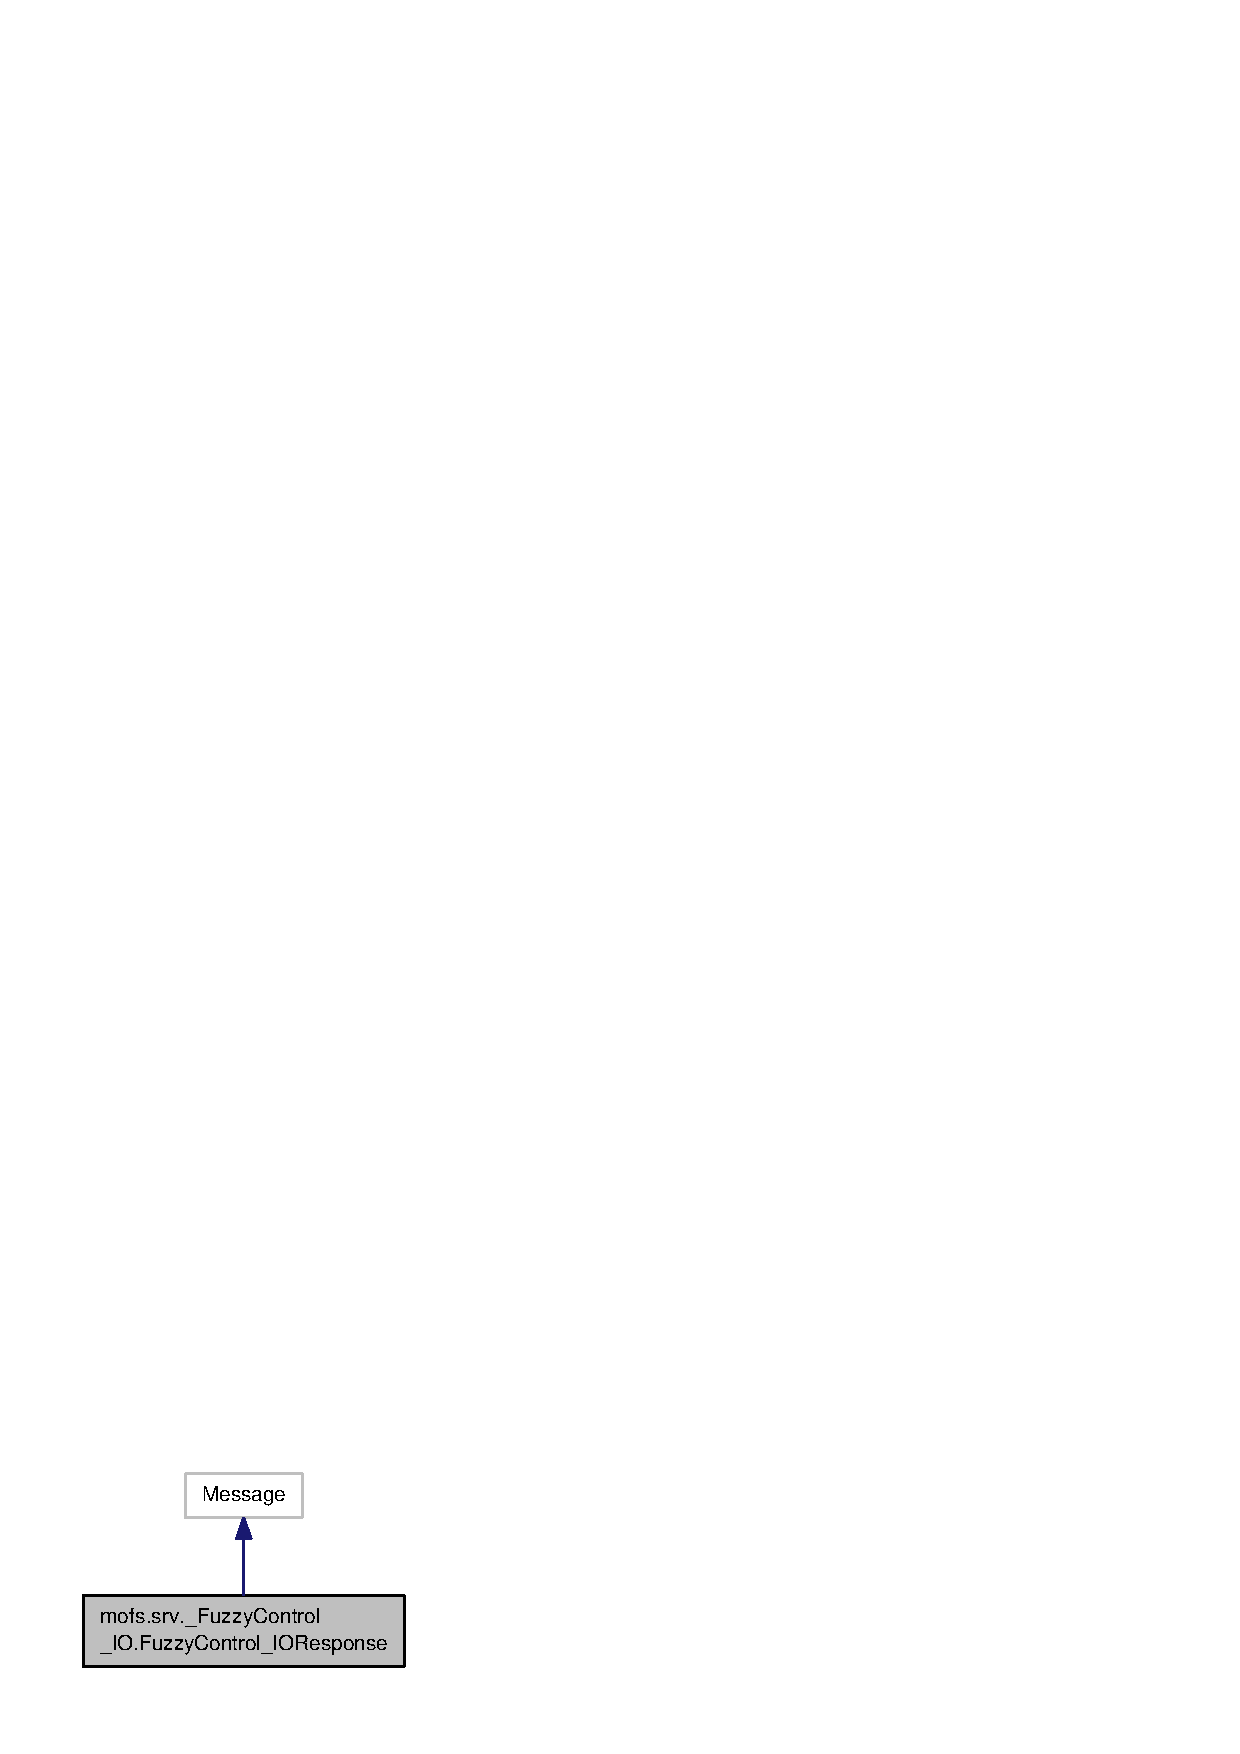
\includegraphics[width=198pt]{classmofs_1_1srv_1_1__FuzzyControl__IO_1_1FuzzyControl__IOResponse__inherit__graph}
\end{center}
\end{figure}
\subsection*{Public Member Functions}
\begin{DoxyCompactItemize}
\item 
def {\bf \-\_\-\-\_\-init\-\_\-\-\_\-}
\item 
def {\bf deserialize}
\item 
def {\bf deserialize\-\_\-numpy}
\item 
def {\bf serialize}
\item 
def {\bf serialize\-\_\-numpy}
\end{DoxyCompactItemize}
\subsection*{Public Attributes}
\begin{DoxyCompactItemize}
\item 
{\bf output}
\end{DoxyCompactItemize}
\subsection*{Private Member Functions}
\begin{DoxyCompactItemize}
\item 
def {\bf \-\_\-get\-\_\-types}
\end{DoxyCompactItemize}
\subsection*{Static Private Attributes}
\begin{DoxyCompactItemize}
\item 
list {\bf \-\_\-\-\_\-slots\-\_\-\-\_\-} = ['{\bf output}']
\item 
string {\bf \-\_\-full\-\_\-text}
\item 
{\bf \-\_\-has\-\_\-header} = False
\item 
string {\bf \-\_\-md5sum} = \char`\"{}dc04e8385a5c2f792e8299232db8e2eb\char`\"{}
\item 
list {\bf \-\_\-slot\-\_\-types} = ['float32']
\item 
string {\bf \-\_\-type} = \char`\"{}mofs/{\bf Fuzzy\-Control\-\_\-\-I\-O\-Response}\char`\"{}
\end{DoxyCompactItemize}


\subsection{Detailed Description}


Definition at line 107 of file \-\_\-\-Fuzzy\-Control\-\_\-\-I\-O.\-py.



\subsection{Constructor \& Destructor Documentation}
\index{mofs\-::srv\-::\-\_\-\-Fuzzy\-Control\-\_\-\-I\-O\-::\-Fuzzy\-Control\-\_\-\-I\-O\-Response@{mofs\-::srv\-::\-\_\-\-Fuzzy\-Control\-\_\-\-I\-O\-::\-Fuzzy\-Control\-\_\-\-I\-O\-Response}!\-\_\-\-\_\-init\-\_\-\-\_\-@{\-\_\-\-\_\-init\-\_\-\-\_\-}}
\index{\-\_\-\-\_\-init\-\_\-\-\_\-@{\-\_\-\-\_\-init\-\_\-\-\_\-}!mofs::srv::_FuzzyControl_IO::FuzzyControl_IOResponse@{mofs\-::srv\-::\-\_\-\-Fuzzy\-Control\-\_\-\-I\-O\-::\-Fuzzy\-Control\-\_\-\-I\-O\-Response}}
\subsubsection[{\-\_\-\-\_\-init\-\_\-\-\_\-}]{\setlength{\rightskip}{0pt plus 5cm}def mofs.\-srv.\-\_\-\-Fuzzy\-Control\-\_\-\-I\-O.\-Fuzzy\-Control\-\_\-\-I\-O\-Response.\-\_\-\-\_\-init\-\_\-\-\_\- (
\begin{DoxyParamCaption}
\item[{}]{self, }
\item[{}]{args, }
\item[{}]{kwds}
\end{DoxyParamCaption}
)}\label{classmofs_1_1srv_1_1__FuzzyControl__IO_1_1FuzzyControl__IOResponse_a2d7d3ef9d98d1bb16142024ba1da3fa1}
\begin{DoxyVerb}Constructor. Any message fields that are implicitly/explicitly
set to None will be assigned a default value. The recommend
use is keyword arguments as this is more robust to future message
changes.  You cannot mix in-order arguments and keyword arguments.

The available fields are:
   output

:param args: complete set of field values, in .msg order
:param kwds: use keyword arguments corresponding to message field names
to set specific fields.
\end{DoxyVerb}
 

Definition at line 118 of file \-\_\-\-Fuzzy\-Control\-\_\-\-I\-O.\-py.



\subsection{Member Function Documentation}
\index{mofs\-::srv\-::\-\_\-\-Fuzzy\-Control\-\_\-\-I\-O\-::\-Fuzzy\-Control\-\_\-\-I\-O\-Response@{mofs\-::srv\-::\-\_\-\-Fuzzy\-Control\-\_\-\-I\-O\-::\-Fuzzy\-Control\-\_\-\-I\-O\-Response}!\-\_\-get\-\_\-types@{\-\_\-get\-\_\-types}}
\index{\-\_\-get\-\_\-types@{\-\_\-get\-\_\-types}!mofs::srv::_FuzzyControl_IO::FuzzyControl_IOResponse@{mofs\-::srv\-::\-\_\-\-Fuzzy\-Control\-\_\-\-I\-O\-::\-Fuzzy\-Control\-\_\-\-I\-O\-Response}}
\subsubsection[{\-\_\-get\-\_\-types}]{\setlength{\rightskip}{0pt plus 5cm}def mofs.\-srv.\-\_\-\-Fuzzy\-Control\-\_\-\-I\-O.\-Fuzzy\-Control\-\_\-\-I\-O\-Response.\-\_\-get\-\_\-types (
\begin{DoxyParamCaption}
\item[{}]{self}
\end{DoxyParamCaption}
)\hspace{0.3cm}{\ttfamily [private]}}\label{classmofs_1_1srv_1_1__FuzzyControl__IO_1_1FuzzyControl__IOResponse_a31394a00145ac330ec7b6b6ae05e82ed}
\begin{DoxyVerb}internal API method
\end{DoxyVerb}
 

Definition at line 140 of file \-\_\-\-Fuzzy\-Control\-\_\-\-I\-O.\-py.

\index{mofs\-::srv\-::\-\_\-\-Fuzzy\-Control\-\_\-\-I\-O\-::\-Fuzzy\-Control\-\_\-\-I\-O\-Response@{mofs\-::srv\-::\-\_\-\-Fuzzy\-Control\-\_\-\-I\-O\-::\-Fuzzy\-Control\-\_\-\-I\-O\-Response}!deserialize@{deserialize}}
\index{deserialize@{deserialize}!mofs::srv::_FuzzyControl_IO::FuzzyControl_IOResponse@{mofs\-::srv\-::\-\_\-\-Fuzzy\-Control\-\_\-\-I\-O\-::\-Fuzzy\-Control\-\_\-\-I\-O\-Response}}
\subsubsection[{deserialize}]{\setlength{\rightskip}{0pt plus 5cm}def mofs.\-srv.\-\_\-\-Fuzzy\-Control\-\_\-\-I\-O.\-Fuzzy\-Control\-\_\-\-I\-O\-Response.\-deserialize (
\begin{DoxyParamCaption}
\item[{}]{self, }
\item[{}]{str}
\end{DoxyParamCaption}
)}\label{classmofs_1_1srv_1_1__FuzzyControl__IO_1_1FuzzyControl__IOResponse_ac22dab46d03f2274f6728692151a17bc}
\begin{DoxyVerb}unpack serialized message in str into this message instance
:param str: byte array of serialized message, ``str``
\end{DoxyVerb}
 

Definition at line 156 of file \-\_\-\-Fuzzy\-Control\-\_\-\-I\-O.\-py.

\index{mofs\-::srv\-::\-\_\-\-Fuzzy\-Control\-\_\-\-I\-O\-::\-Fuzzy\-Control\-\_\-\-I\-O\-Response@{mofs\-::srv\-::\-\_\-\-Fuzzy\-Control\-\_\-\-I\-O\-::\-Fuzzy\-Control\-\_\-\-I\-O\-Response}!deserialize\-\_\-numpy@{deserialize\-\_\-numpy}}
\index{deserialize\-\_\-numpy@{deserialize\-\_\-numpy}!mofs::srv::_FuzzyControl_IO::FuzzyControl_IOResponse@{mofs\-::srv\-::\-\_\-\-Fuzzy\-Control\-\_\-\-I\-O\-::\-Fuzzy\-Control\-\_\-\-I\-O\-Response}}
\subsubsection[{deserialize\-\_\-numpy}]{\setlength{\rightskip}{0pt plus 5cm}def mofs.\-srv.\-\_\-\-Fuzzy\-Control\-\_\-\-I\-O.\-Fuzzy\-Control\-\_\-\-I\-O\-Response.\-deserialize\-\_\-numpy (
\begin{DoxyParamCaption}
\item[{}]{self, }
\item[{}]{str, }
\item[{}]{numpy}
\end{DoxyParamCaption}
)}\label{classmofs_1_1srv_1_1__FuzzyControl__IO_1_1FuzzyControl__IOResponse_afcf02fa0ee1f2c25edff91920c2fce9b}
\begin{DoxyVerb}unpack serialized message in str into this message instance using numpy for array types
:param str: byte array of serialized message, ``str``
:param numpy: numpy python module
\end{DoxyVerb}
 

Definition at line 182 of file \-\_\-\-Fuzzy\-Control\-\_\-\-I\-O.\-py.

\index{mofs\-::srv\-::\-\_\-\-Fuzzy\-Control\-\_\-\-I\-O\-::\-Fuzzy\-Control\-\_\-\-I\-O\-Response@{mofs\-::srv\-::\-\_\-\-Fuzzy\-Control\-\_\-\-I\-O\-::\-Fuzzy\-Control\-\_\-\-I\-O\-Response}!serialize@{serialize}}
\index{serialize@{serialize}!mofs::srv::_FuzzyControl_IO::FuzzyControl_IOResponse@{mofs\-::srv\-::\-\_\-\-Fuzzy\-Control\-\_\-\-I\-O\-::\-Fuzzy\-Control\-\_\-\-I\-O\-Response}}
\subsubsection[{serialize}]{\setlength{\rightskip}{0pt plus 5cm}def mofs.\-srv.\-\_\-\-Fuzzy\-Control\-\_\-\-I\-O.\-Fuzzy\-Control\-\_\-\-I\-O\-Response.\-serialize (
\begin{DoxyParamCaption}
\item[{}]{self, }
\item[{}]{buff}
\end{DoxyParamCaption}
)}\label{classmofs_1_1srv_1_1__FuzzyControl__IO_1_1FuzzyControl__IOResponse_a093836f59b7482c9cad1751e903cdff5}
\begin{DoxyVerb}serialize message into buffer
:param buff: buffer, ``StringIO``
\end{DoxyVerb}
 

Definition at line 146 of file \-\_\-\-Fuzzy\-Control\-\_\-\-I\-O.\-py.

\index{mofs\-::srv\-::\-\_\-\-Fuzzy\-Control\-\_\-\-I\-O\-::\-Fuzzy\-Control\-\_\-\-I\-O\-Response@{mofs\-::srv\-::\-\_\-\-Fuzzy\-Control\-\_\-\-I\-O\-::\-Fuzzy\-Control\-\_\-\-I\-O\-Response}!serialize\-\_\-numpy@{serialize\-\_\-numpy}}
\index{serialize\-\_\-numpy@{serialize\-\_\-numpy}!mofs::srv::_FuzzyControl_IO::FuzzyControl_IOResponse@{mofs\-::srv\-::\-\_\-\-Fuzzy\-Control\-\_\-\-I\-O\-::\-Fuzzy\-Control\-\_\-\-I\-O\-Response}}
\subsubsection[{serialize\-\_\-numpy}]{\setlength{\rightskip}{0pt plus 5cm}def mofs.\-srv.\-\_\-\-Fuzzy\-Control\-\_\-\-I\-O.\-Fuzzy\-Control\-\_\-\-I\-O\-Response.\-serialize\-\_\-numpy (
\begin{DoxyParamCaption}
\item[{}]{self, }
\item[{}]{buff, }
\item[{}]{numpy}
\end{DoxyParamCaption}
)}\label{classmofs_1_1srv_1_1__FuzzyControl__IO_1_1FuzzyControl__IOResponse_a5cfd549b0e78975d58d063d299e42d39}
\begin{DoxyVerb}serialize message with numpy array types into buffer
:param buff: buffer, ``StringIO``
:param numpy: numpy python module
\end{DoxyVerb}
 

Definition at line 171 of file \-\_\-\-Fuzzy\-Control\-\_\-\-I\-O.\-py.



\subsection{Member Data Documentation}
\index{mofs\-::srv\-::\-\_\-\-Fuzzy\-Control\-\_\-\-I\-O\-::\-Fuzzy\-Control\-\_\-\-I\-O\-Response@{mofs\-::srv\-::\-\_\-\-Fuzzy\-Control\-\_\-\-I\-O\-::\-Fuzzy\-Control\-\_\-\-I\-O\-Response}!\-\_\-\-\_\-slots\-\_\-\-\_\-@{\-\_\-\-\_\-slots\-\_\-\-\_\-}}
\index{\-\_\-\-\_\-slots\-\_\-\-\_\-@{\-\_\-\-\_\-slots\-\_\-\-\_\-}!mofs::srv::_FuzzyControl_IO::FuzzyControl_IOResponse@{mofs\-::srv\-::\-\_\-\-Fuzzy\-Control\-\_\-\-I\-O\-::\-Fuzzy\-Control\-\_\-\-I\-O\-Response}}
\subsubsection[{\-\_\-\-\_\-slots\-\_\-\-\_\-}]{\setlength{\rightskip}{0pt plus 5cm}list mofs.\-srv.\-\_\-\-Fuzzy\-Control\-\_\-\-I\-O.\-Fuzzy\-Control\-\_\-\-I\-O\-Response.\-\_\-\-\_\-slots\-\_\-\-\_\- = ['{\bf output}']\hspace{0.3cm}{\ttfamily [static]}, {\ttfamily [private]}}\label{classmofs_1_1srv_1_1__FuzzyControl__IO_1_1FuzzyControl__IOResponse_a8d4942d47d516686a56b4c7da6689450}


Definition at line 115 of file \-\_\-\-Fuzzy\-Control\-\_\-\-I\-O.\-py.

\index{mofs\-::srv\-::\-\_\-\-Fuzzy\-Control\-\_\-\-I\-O\-::\-Fuzzy\-Control\-\_\-\-I\-O\-Response@{mofs\-::srv\-::\-\_\-\-Fuzzy\-Control\-\_\-\-I\-O\-::\-Fuzzy\-Control\-\_\-\-I\-O\-Response}!\-\_\-full\-\_\-text@{\-\_\-full\-\_\-text}}
\index{\-\_\-full\-\_\-text@{\-\_\-full\-\_\-text}!mofs::srv::_FuzzyControl_IO::FuzzyControl_IOResponse@{mofs\-::srv\-::\-\_\-\-Fuzzy\-Control\-\_\-\-I\-O\-::\-Fuzzy\-Control\-\_\-\-I\-O\-Response}}
\subsubsection[{\-\_\-full\-\_\-text}]{\setlength{\rightskip}{0pt plus 5cm}string mofs.\-srv.\-\_\-\-Fuzzy\-Control\-\_\-\-I\-O.\-Fuzzy\-Control\-\_\-\-I\-O\-Response.\-\_\-full\-\_\-text\hspace{0.3cm}{\ttfamily [static]}, {\ttfamily [private]}}\label{classmofs_1_1srv_1_1__FuzzyControl__IO_1_1FuzzyControl__IOResponse_ad6cbdc0c453302b9bf497e7d698e75a2}
{\bfseries Initial value\-:}
\begin{DoxyCode}
1 = \textcolor{stringliteral}{"""float32 output}
2 \textcolor{stringliteral}{}
3 \textcolor{stringliteral}{}
4 \textcolor{stringliteral}{"""}
\end{DoxyCode}


Definition at line 111 of file \-\_\-\-Fuzzy\-Control\-\_\-\-I\-O.\-py.

\index{mofs\-::srv\-::\-\_\-\-Fuzzy\-Control\-\_\-\-I\-O\-::\-Fuzzy\-Control\-\_\-\-I\-O\-Response@{mofs\-::srv\-::\-\_\-\-Fuzzy\-Control\-\_\-\-I\-O\-::\-Fuzzy\-Control\-\_\-\-I\-O\-Response}!\-\_\-has\-\_\-header@{\-\_\-has\-\_\-header}}
\index{\-\_\-has\-\_\-header@{\-\_\-has\-\_\-header}!mofs::srv::_FuzzyControl_IO::FuzzyControl_IOResponse@{mofs\-::srv\-::\-\_\-\-Fuzzy\-Control\-\_\-\-I\-O\-::\-Fuzzy\-Control\-\_\-\-I\-O\-Response}}
\subsubsection[{\-\_\-has\-\_\-header}]{\setlength{\rightskip}{0pt plus 5cm}mofs.\-srv.\-\_\-\-Fuzzy\-Control\-\_\-\-I\-O.\-Fuzzy\-Control\-\_\-\-I\-O\-Response.\-\_\-has\-\_\-header = False\hspace{0.3cm}{\ttfamily [static]}, {\ttfamily [private]}}\label{classmofs_1_1srv_1_1__FuzzyControl__IO_1_1FuzzyControl__IOResponse_a8cf05a743e4ece21b7e0eaedec9e6f24}


Definition at line 110 of file \-\_\-\-Fuzzy\-Control\-\_\-\-I\-O.\-py.

\index{mofs\-::srv\-::\-\_\-\-Fuzzy\-Control\-\_\-\-I\-O\-::\-Fuzzy\-Control\-\_\-\-I\-O\-Response@{mofs\-::srv\-::\-\_\-\-Fuzzy\-Control\-\_\-\-I\-O\-::\-Fuzzy\-Control\-\_\-\-I\-O\-Response}!\-\_\-md5sum@{\-\_\-md5sum}}
\index{\-\_\-md5sum@{\-\_\-md5sum}!mofs::srv::_FuzzyControl_IO::FuzzyControl_IOResponse@{mofs\-::srv\-::\-\_\-\-Fuzzy\-Control\-\_\-\-I\-O\-::\-Fuzzy\-Control\-\_\-\-I\-O\-Response}}
\subsubsection[{\-\_\-md5sum}]{\setlength{\rightskip}{0pt plus 5cm}string mofs.\-srv.\-\_\-\-Fuzzy\-Control\-\_\-\-I\-O.\-Fuzzy\-Control\-\_\-\-I\-O\-Response.\-\_\-md5sum = \char`\"{}dc04e8385a5c2f792e8299232db8e2eb\char`\"{}\hspace{0.3cm}{\ttfamily [static]}, {\ttfamily [private]}}\label{classmofs_1_1srv_1_1__FuzzyControl__IO_1_1FuzzyControl__IOResponse_a0451937918c851d319e012d5dbc2a87b}


Definition at line 108 of file \-\_\-\-Fuzzy\-Control\-\_\-\-I\-O.\-py.

\index{mofs\-::srv\-::\-\_\-\-Fuzzy\-Control\-\_\-\-I\-O\-::\-Fuzzy\-Control\-\_\-\-I\-O\-Response@{mofs\-::srv\-::\-\_\-\-Fuzzy\-Control\-\_\-\-I\-O\-::\-Fuzzy\-Control\-\_\-\-I\-O\-Response}!\-\_\-slot\-\_\-types@{\-\_\-slot\-\_\-types}}
\index{\-\_\-slot\-\_\-types@{\-\_\-slot\-\_\-types}!mofs::srv::_FuzzyControl_IO::FuzzyControl_IOResponse@{mofs\-::srv\-::\-\_\-\-Fuzzy\-Control\-\_\-\-I\-O\-::\-Fuzzy\-Control\-\_\-\-I\-O\-Response}}
\subsubsection[{\-\_\-slot\-\_\-types}]{\setlength{\rightskip}{0pt plus 5cm}list mofs.\-srv.\-\_\-\-Fuzzy\-Control\-\_\-\-I\-O.\-Fuzzy\-Control\-\_\-\-I\-O\-Response.\-\_\-slot\-\_\-types = ['float32']\hspace{0.3cm}{\ttfamily [static]}, {\ttfamily [private]}}\label{classmofs_1_1srv_1_1__FuzzyControl__IO_1_1FuzzyControl__IOResponse_a90119b51240aff2a66e2bebc9cc4e9de}


Definition at line 116 of file \-\_\-\-Fuzzy\-Control\-\_\-\-I\-O.\-py.

\index{mofs\-::srv\-::\-\_\-\-Fuzzy\-Control\-\_\-\-I\-O\-::\-Fuzzy\-Control\-\_\-\-I\-O\-Response@{mofs\-::srv\-::\-\_\-\-Fuzzy\-Control\-\_\-\-I\-O\-::\-Fuzzy\-Control\-\_\-\-I\-O\-Response}!\-\_\-type@{\-\_\-type}}
\index{\-\_\-type@{\-\_\-type}!mofs::srv::_FuzzyControl_IO::FuzzyControl_IOResponse@{mofs\-::srv\-::\-\_\-\-Fuzzy\-Control\-\_\-\-I\-O\-::\-Fuzzy\-Control\-\_\-\-I\-O\-Response}}
\subsubsection[{\-\_\-type}]{\setlength{\rightskip}{0pt plus 5cm}string mofs.\-srv.\-\_\-\-Fuzzy\-Control\-\_\-\-I\-O.\-Fuzzy\-Control\-\_\-\-I\-O\-Response.\-\_\-type = \char`\"{}mofs/{\bf Fuzzy\-Control\-\_\-\-I\-O\-Response}\char`\"{}\hspace{0.3cm}{\ttfamily [static]}, {\ttfamily [private]}}\label{classmofs_1_1srv_1_1__FuzzyControl__IO_1_1FuzzyControl__IOResponse_a88e212ff3924178893427c2143e512f7}


Definition at line 109 of file \-\_\-\-Fuzzy\-Control\-\_\-\-I\-O.\-py.

\index{mofs\-::srv\-::\-\_\-\-Fuzzy\-Control\-\_\-\-I\-O\-::\-Fuzzy\-Control\-\_\-\-I\-O\-Response@{mofs\-::srv\-::\-\_\-\-Fuzzy\-Control\-\_\-\-I\-O\-::\-Fuzzy\-Control\-\_\-\-I\-O\-Response}!output@{output}}
\index{output@{output}!mofs::srv::_FuzzyControl_IO::FuzzyControl_IOResponse@{mofs\-::srv\-::\-\_\-\-Fuzzy\-Control\-\_\-\-I\-O\-::\-Fuzzy\-Control\-\_\-\-I\-O\-Response}}
\subsubsection[{output}]{\setlength{\rightskip}{0pt plus 5cm}mofs.\-srv.\-\_\-\-Fuzzy\-Control\-\_\-\-I\-O.\-Fuzzy\-Control\-\_\-\-I\-O\-Response.\-output}\label{classmofs_1_1srv_1_1__FuzzyControl__IO_1_1FuzzyControl__IOResponse_a348ed3b41b66440928a313a0d3b7c986}


Definition at line 136 of file \-\_\-\-Fuzzy\-Control\-\_\-\-I\-O.\-py.



The documentation for this class was generated from the following file\-:\begin{DoxyCompactItemize}
\item 
{\bf \-\_\-\-Fuzzy\-Control\-\_\-\-I\-O.\-py}\end{DoxyCompactItemize}

\section{mofs\-:\-:Fuzzy\-Control\-\_\-\-I\-O\-Response\-\_\-$<$ Container\-Allocator $>$ Struct Template Reference}
\label{structmofs_1_1FuzzyControl__IOResponse__}\index{mofs\-::\-Fuzzy\-Control\-\_\-\-I\-O\-Response\-\_\-$<$ Container\-Allocator $>$@{mofs\-::\-Fuzzy\-Control\-\_\-\-I\-O\-Response\-\_\-$<$ Container\-Allocator $>$}}


{\ttfamily \#include $<$Fuzzy\-Control\-\_\-\-I\-O.\-h$>$}

\subsection*{Public Types}
\begin{DoxyCompactItemize}
\item 
typedef float {\bf \-\_\-output\-\_\-type}
\item 
typedef boost\-::shared\-\_\-ptr\\*
$<$ \-::{\bf mofs\-::\-Fuzzy\-Control\-\_\-\-I\-O\-Response\-\_\-}\\*
$<$ Container\-Allocator $>$ const  $>$ {\bf Const\-Ptr}
\item 
typedef boost\-::shared\-\_\-ptr\\*
$<$ \-::{\bf mofs\-::\-Fuzzy\-Control\-\_\-\-I\-O\-Response\-\_\-}\\*
$<$ Container\-Allocator $>$ $>$ {\bf Ptr}
\item 
typedef \\*
{\bf Fuzzy\-Control\-\_\-\-I\-O\-Response\-\_\-}\\*
$<$ Container\-Allocator $>$ {\bf Type}
\end{DoxyCompactItemize}
\subsection*{Public Member Functions}
\begin{DoxyCompactItemize}
\item 
{\bf Fuzzy\-Control\-\_\-\-I\-O\-Response\-\_\-} ()
\item 
{\bf Fuzzy\-Control\-\_\-\-I\-O\-Response\-\_\-} (const Container\-Allocator \&\-\_\-alloc)
\end{DoxyCompactItemize}
\subsection*{Public Attributes}
\begin{DoxyCompactItemize}
\item 
boost\-::shared\-\_\-ptr$<$ std\-::map\\*
$<$ std\-::string, std\-::string $>$ $>$ {\bf \-\_\-\-\_\-connection\-\_\-header}
\item 
float {\bf output}
\end{DoxyCompactItemize}


\subsection{Detailed Description}
\subsubsection*{template$<$class Container\-Allocator$>$struct mofs\-::\-Fuzzy\-Control\-\_\-\-I\-O\-Response\-\_\-$<$ Container\-Allocator $>$}



Definition at line 55 of file Fuzzy\-Control\-\_\-\-I\-O.\-h.



\subsection{Member Typedef Documentation}
\index{mofs\-::\-Fuzzy\-Control\-\_\-\-I\-O\-Response\-\_\-@{mofs\-::\-Fuzzy\-Control\-\_\-\-I\-O\-Response\-\_\-}!\-\_\-output\-\_\-type@{\-\_\-output\-\_\-type}}
\index{\-\_\-output\-\_\-type@{\-\_\-output\-\_\-type}!mofs::FuzzyControl_IOResponse_@{mofs\-::\-Fuzzy\-Control\-\_\-\-I\-O\-Response\-\_\-}}
\subsubsection[{\-\_\-output\-\_\-type}]{\setlength{\rightskip}{0pt plus 5cm}template$<$class Container\-Allocator $>$ typedef float {\bf mofs\-::\-Fuzzy\-Control\-\_\-\-I\-O\-Response\-\_\-}$<$ Container\-Allocator $>$\-::{\bf \-\_\-output\-\_\-type}}\label{structmofs_1_1FuzzyControl__IOResponse___a96489f175001c823c6cbd85d2219a033}


Definition at line 68 of file Fuzzy\-Control\-\_\-\-I\-O.\-h.

\index{mofs\-::\-Fuzzy\-Control\-\_\-\-I\-O\-Response\-\_\-@{mofs\-::\-Fuzzy\-Control\-\_\-\-I\-O\-Response\-\_\-}!Const\-Ptr@{Const\-Ptr}}
\index{Const\-Ptr@{Const\-Ptr}!mofs::FuzzyControl_IOResponse_@{mofs\-::\-Fuzzy\-Control\-\_\-\-I\-O\-Response\-\_\-}}
\subsubsection[{Const\-Ptr}]{\setlength{\rightskip}{0pt plus 5cm}template$<$class Container\-Allocator $>$ typedef boost\-::shared\-\_\-ptr$<$ \-::{\bf mofs\-::\-Fuzzy\-Control\-\_\-\-I\-O\-Response\-\_\-}$<$Container\-Allocator$>$ const$>$ {\bf mofs\-::\-Fuzzy\-Control\-\_\-\-I\-O\-Response\-\_\-}$<$ Container\-Allocator $>$\-::{\bf Const\-Ptr}}\label{structmofs_1_1FuzzyControl__IOResponse___a5aa6922243e5b5a2fe921fc69ad483b5}


Definition at line 73 of file Fuzzy\-Control\-\_\-\-I\-O.\-h.

\index{mofs\-::\-Fuzzy\-Control\-\_\-\-I\-O\-Response\-\_\-@{mofs\-::\-Fuzzy\-Control\-\_\-\-I\-O\-Response\-\_\-}!Ptr@{Ptr}}
\index{Ptr@{Ptr}!mofs::FuzzyControl_IOResponse_@{mofs\-::\-Fuzzy\-Control\-\_\-\-I\-O\-Response\-\_\-}}
\subsubsection[{Ptr}]{\setlength{\rightskip}{0pt plus 5cm}template$<$class Container\-Allocator $>$ typedef boost\-::shared\-\_\-ptr$<$ \-::{\bf mofs\-::\-Fuzzy\-Control\-\_\-\-I\-O\-Response\-\_\-}$<$Container\-Allocator$>$ $>$ {\bf mofs\-::\-Fuzzy\-Control\-\_\-\-I\-O\-Response\-\_\-}$<$ Container\-Allocator $>$\-::{\bf Ptr}}\label{structmofs_1_1FuzzyControl__IOResponse___a2713784b433c3c46a9e97dc428c3b31e}


Definition at line 72 of file Fuzzy\-Control\-\_\-\-I\-O.\-h.

\index{mofs\-::\-Fuzzy\-Control\-\_\-\-I\-O\-Response\-\_\-@{mofs\-::\-Fuzzy\-Control\-\_\-\-I\-O\-Response\-\_\-}!Type@{Type}}
\index{Type@{Type}!mofs::FuzzyControl_IOResponse_@{mofs\-::\-Fuzzy\-Control\-\_\-\-I\-O\-Response\-\_\-}}
\subsubsection[{Type}]{\setlength{\rightskip}{0pt plus 5cm}template$<$class Container\-Allocator $>$ typedef {\bf Fuzzy\-Control\-\_\-\-I\-O\-Response\-\_\-}$<$Container\-Allocator$>$ {\bf mofs\-::\-Fuzzy\-Control\-\_\-\-I\-O\-Response\-\_\-}$<$ Container\-Allocator $>$\-::{\bf Type}}\label{structmofs_1_1FuzzyControl__IOResponse___ae3711d2092898c571bd42cdbc4df8eb4}


Definition at line 56 of file Fuzzy\-Control\-\_\-\-I\-O.\-h.



\subsection{Constructor \& Destructor Documentation}
\index{mofs\-::\-Fuzzy\-Control\-\_\-\-I\-O\-Response\-\_\-@{mofs\-::\-Fuzzy\-Control\-\_\-\-I\-O\-Response\-\_\-}!Fuzzy\-Control\-\_\-\-I\-O\-Response\-\_\-@{Fuzzy\-Control\-\_\-\-I\-O\-Response\-\_\-}}
\index{Fuzzy\-Control\-\_\-\-I\-O\-Response\-\_\-@{Fuzzy\-Control\-\_\-\-I\-O\-Response\-\_\-}!mofs::FuzzyControl_IOResponse_@{mofs\-::\-Fuzzy\-Control\-\_\-\-I\-O\-Response\-\_\-}}
\subsubsection[{Fuzzy\-Control\-\_\-\-I\-O\-Response\-\_\-}]{\setlength{\rightskip}{0pt plus 5cm}template$<$class Container\-Allocator $>$ {\bf mofs\-::\-Fuzzy\-Control\-\_\-\-I\-O\-Response\-\_\-}$<$ Container\-Allocator $>$\-::{\bf Fuzzy\-Control\-\_\-\-I\-O\-Response\-\_\-} (
\begin{DoxyParamCaption}
{}
\end{DoxyParamCaption}
)\hspace{0.3cm}{\ttfamily [inline]}}\label{structmofs_1_1FuzzyControl__IOResponse___a80116670b56d0dac368c5aa52313c8a5}


Definition at line 58 of file Fuzzy\-Control\-\_\-\-I\-O.\-h.

\index{mofs\-::\-Fuzzy\-Control\-\_\-\-I\-O\-Response\-\_\-@{mofs\-::\-Fuzzy\-Control\-\_\-\-I\-O\-Response\-\_\-}!Fuzzy\-Control\-\_\-\-I\-O\-Response\-\_\-@{Fuzzy\-Control\-\_\-\-I\-O\-Response\-\_\-}}
\index{Fuzzy\-Control\-\_\-\-I\-O\-Response\-\_\-@{Fuzzy\-Control\-\_\-\-I\-O\-Response\-\_\-}!mofs::FuzzyControl_IOResponse_@{mofs\-::\-Fuzzy\-Control\-\_\-\-I\-O\-Response\-\_\-}}
\subsubsection[{Fuzzy\-Control\-\_\-\-I\-O\-Response\-\_\-}]{\setlength{\rightskip}{0pt plus 5cm}template$<$class Container\-Allocator $>$ {\bf mofs\-::\-Fuzzy\-Control\-\_\-\-I\-O\-Response\-\_\-}$<$ Container\-Allocator $>$\-::{\bf Fuzzy\-Control\-\_\-\-I\-O\-Response\-\_\-} (
\begin{DoxyParamCaption}
\item[{const Container\-Allocator \&}]{\-\_\-alloc}
\end{DoxyParamCaption}
)\hspace{0.3cm}{\ttfamily [inline]}}\label{structmofs_1_1FuzzyControl__IOResponse___a7e9b53ba18ce5fe67883e7daabd8dd4a}


Definition at line 63 of file Fuzzy\-Control\-\_\-\-I\-O.\-h.



\subsection{Member Data Documentation}
\index{mofs\-::\-Fuzzy\-Control\-\_\-\-I\-O\-Response\-\_\-@{mofs\-::\-Fuzzy\-Control\-\_\-\-I\-O\-Response\-\_\-}!\-\_\-\-\_\-connection\-\_\-header@{\-\_\-\-\_\-connection\-\_\-header}}
\index{\-\_\-\-\_\-connection\-\_\-header@{\-\_\-\-\_\-connection\-\_\-header}!mofs::FuzzyControl_IOResponse_@{mofs\-::\-Fuzzy\-Control\-\_\-\-I\-O\-Response\-\_\-}}
\subsubsection[{\-\_\-\-\_\-connection\-\_\-header}]{\setlength{\rightskip}{0pt plus 5cm}template$<$class Container\-Allocator $>$ boost\-::shared\-\_\-ptr$<$std\-::map$<$std\-::string, std\-::string$>$ $>$ {\bf mofs\-::\-Fuzzy\-Control\-\_\-\-I\-O\-Response\-\_\-}$<$ Container\-Allocator $>$\-::\-\_\-\-\_\-connection\-\_\-header}\label{structmofs_1_1FuzzyControl__IOResponse___ad6ab248cfd51047a96842bb6810f9b02}


Definition at line 74 of file Fuzzy\-Control\-\_\-\-I\-O.\-h.

\index{mofs\-::\-Fuzzy\-Control\-\_\-\-I\-O\-Response\-\_\-@{mofs\-::\-Fuzzy\-Control\-\_\-\-I\-O\-Response\-\_\-}!output@{output}}
\index{output@{output}!mofs::FuzzyControl_IOResponse_@{mofs\-::\-Fuzzy\-Control\-\_\-\-I\-O\-Response\-\_\-}}
\subsubsection[{output}]{\setlength{\rightskip}{0pt plus 5cm}template$<$class Container\-Allocator $>$ float {\bf mofs\-::\-Fuzzy\-Control\-\_\-\-I\-O\-Response\-\_\-}$<$ Container\-Allocator $>$\-::output}\label{structmofs_1_1FuzzyControl__IOResponse___ac5471a7e04482683f9b1802edb006c60}


Definition at line 69 of file Fuzzy\-Control\-\_\-\-I\-O.\-h.



The documentation for this struct was generated from the following file\-:\begin{DoxyCompactItemize}
\item 
{\bf Fuzzy\-Control\-\_\-\-I\-O.\-h}\end{DoxyCompactItemize}

\section{ros\-:\-:message\-\_\-traits\-:\-:Is\-Fixed\-Size$<$ \-:\-:mofs\-:\-:Fuzzy\-Control\-\_\-\-I\-O\-Request\-\_\-$<$ Container\-Allocator $>$ $>$ Struct Template Reference}
\label{structros_1_1message__traits_1_1IsFixedSize_3_01_1_1mofs_1_1FuzzyControl__IORequest___3_01ContainerAllocator_01_4_01_4}\index{ros\-::message\-\_\-traits\-::\-Is\-Fixed\-Size$<$ \-::mofs\-::\-Fuzzy\-Control\-\_\-\-I\-O\-Request\-\_\-$<$ Container\-Allocator $>$ $>$@{ros\-::message\-\_\-traits\-::\-Is\-Fixed\-Size$<$ \-::mofs\-::\-Fuzzy\-Control\-\_\-\-I\-O\-Request\-\_\-$<$ Container\-Allocator $>$ $>$}}


{\ttfamily \#include $<$Fuzzy\-Control\-\_\-\-I\-O.\-h$>$}



Inheritance diagram for ros\-:\-:message\-\_\-traits\-:\-:Is\-Fixed\-Size$<$ \-:\-:mofs\-:\-:Fuzzy\-Control\-\_\-\-I\-O\-Request\-\_\-$<$ Container\-Allocator $>$ $>$\-:\nopagebreak
\begin{figure}[H]
\begin{center}
\leavevmode
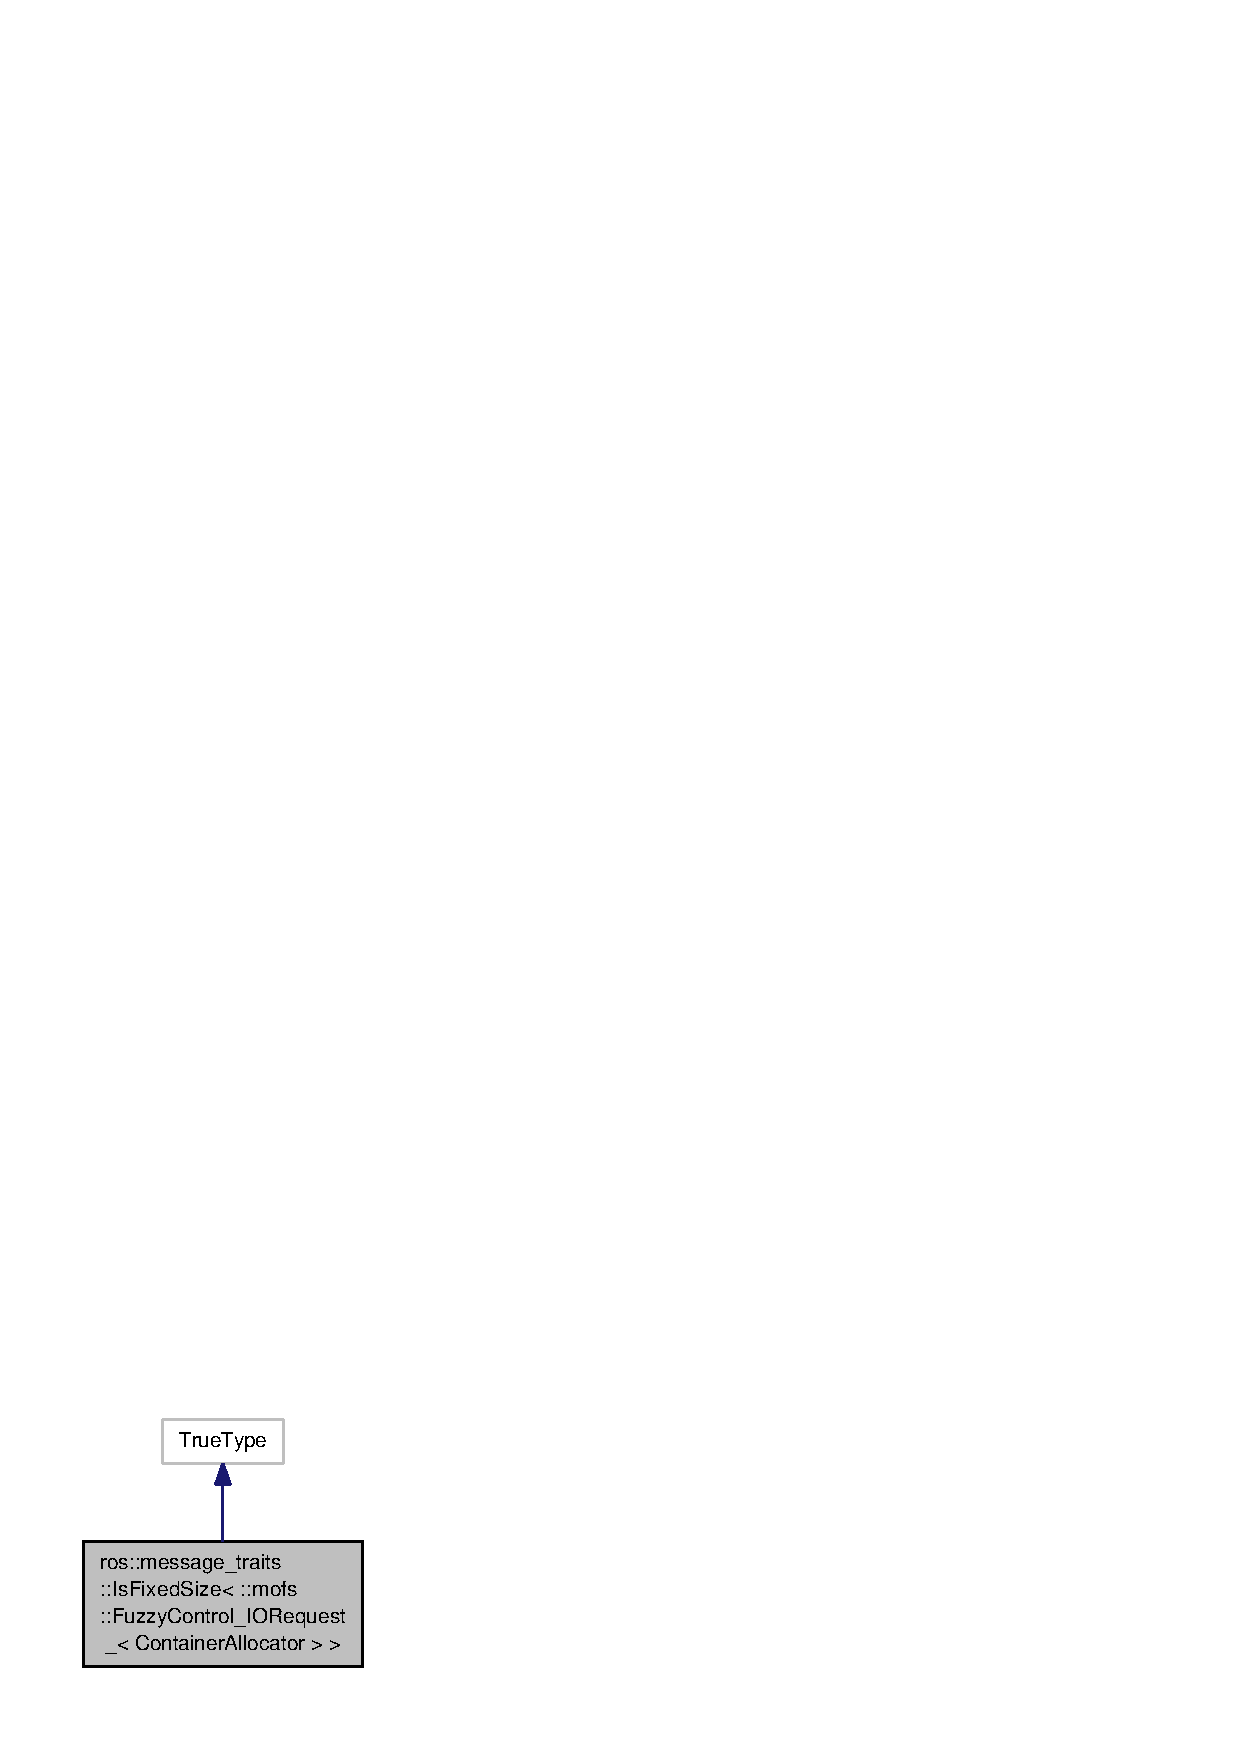
\includegraphics[width=178pt]{structros_1_1message__traits_1_1IsFixedSize_3_01_1_1mofs_1_1FuzzyControl__IORequest___3_01Contai4220f4dba693801f30c17e41c646c6a4}
\end{center}
\end{figure}


\subsection{Detailed Description}
\subsubsection*{template$<$class Container\-Allocator$>$struct ros\-::message\-\_\-traits\-::\-Is\-Fixed\-Size$<$ \-::mofs\-::\-Fuzzy\-Control\-\_\-\-I\-O\-Request\-\_\-$<$ Container\-Allocator $>$ $>$}



Definition at line 135 of file Fuzzy\-Control\-\_\-\-I\-O.\-h.



The documentation for this struct was generated from the following file\-:\begin{DoxyCompactItemize}
\item 
{\bf Fuzzy\-Control\-\_\-\-I\-O.\-h}\end{DoxyCompactItemize}

\section{ros\-:\-:message\-\_\-traits\-:\-:Is\-Fixed\-Size$<$ \-:\-:mofs\-:\-:Fuzzy\-Control\-\_\-\-I\-O\-Response\-\_\-$<$ Container\-Allocator $>$ $>$ Struct Template Reference}
\label{structros_1_1message__traits_1_1IsFixedSize_3_01_1_1mofs_1_1FuzzyControl__IOResponse___3_01ContainerAllocator_01_4_01_4}\index{ros\-::message\-\_\-traits\-::\-Is\-Fixed\-Size$<$ \-::mofs\-::\-Fuzzy\-Control\-\_\-\-I\-O\-Response\-\_\-$<$ Container\-Allocator $>$ $>$@{ros\-::message\-\_\-traits\-::\-Is\-Fixed\-Size$<$ \-::mofs\-::\-Fuzzy\-Control\-\_\-\-I\-O\-Response\-\_\-$<$ Container\-Allocator $>$ $>$}}


{\ttfamily \#include $<$Fuzzy\-Control\-\_\-\-I\-O.\-h$>$}



Inheritance diagram for ros\-:\-:message\-\_\-traits\-:\-:Is\-Fixed\-Size$<$ \-:\-:mofs\-:\-:Fuzzy\-Control\-\_\-\-I\-O\-Response\-\_\-$<$ Container\-Allocator $>$ $>$\-:\nopagebreak
\begin{figure}[H]
\begin{center}
\leavevmode
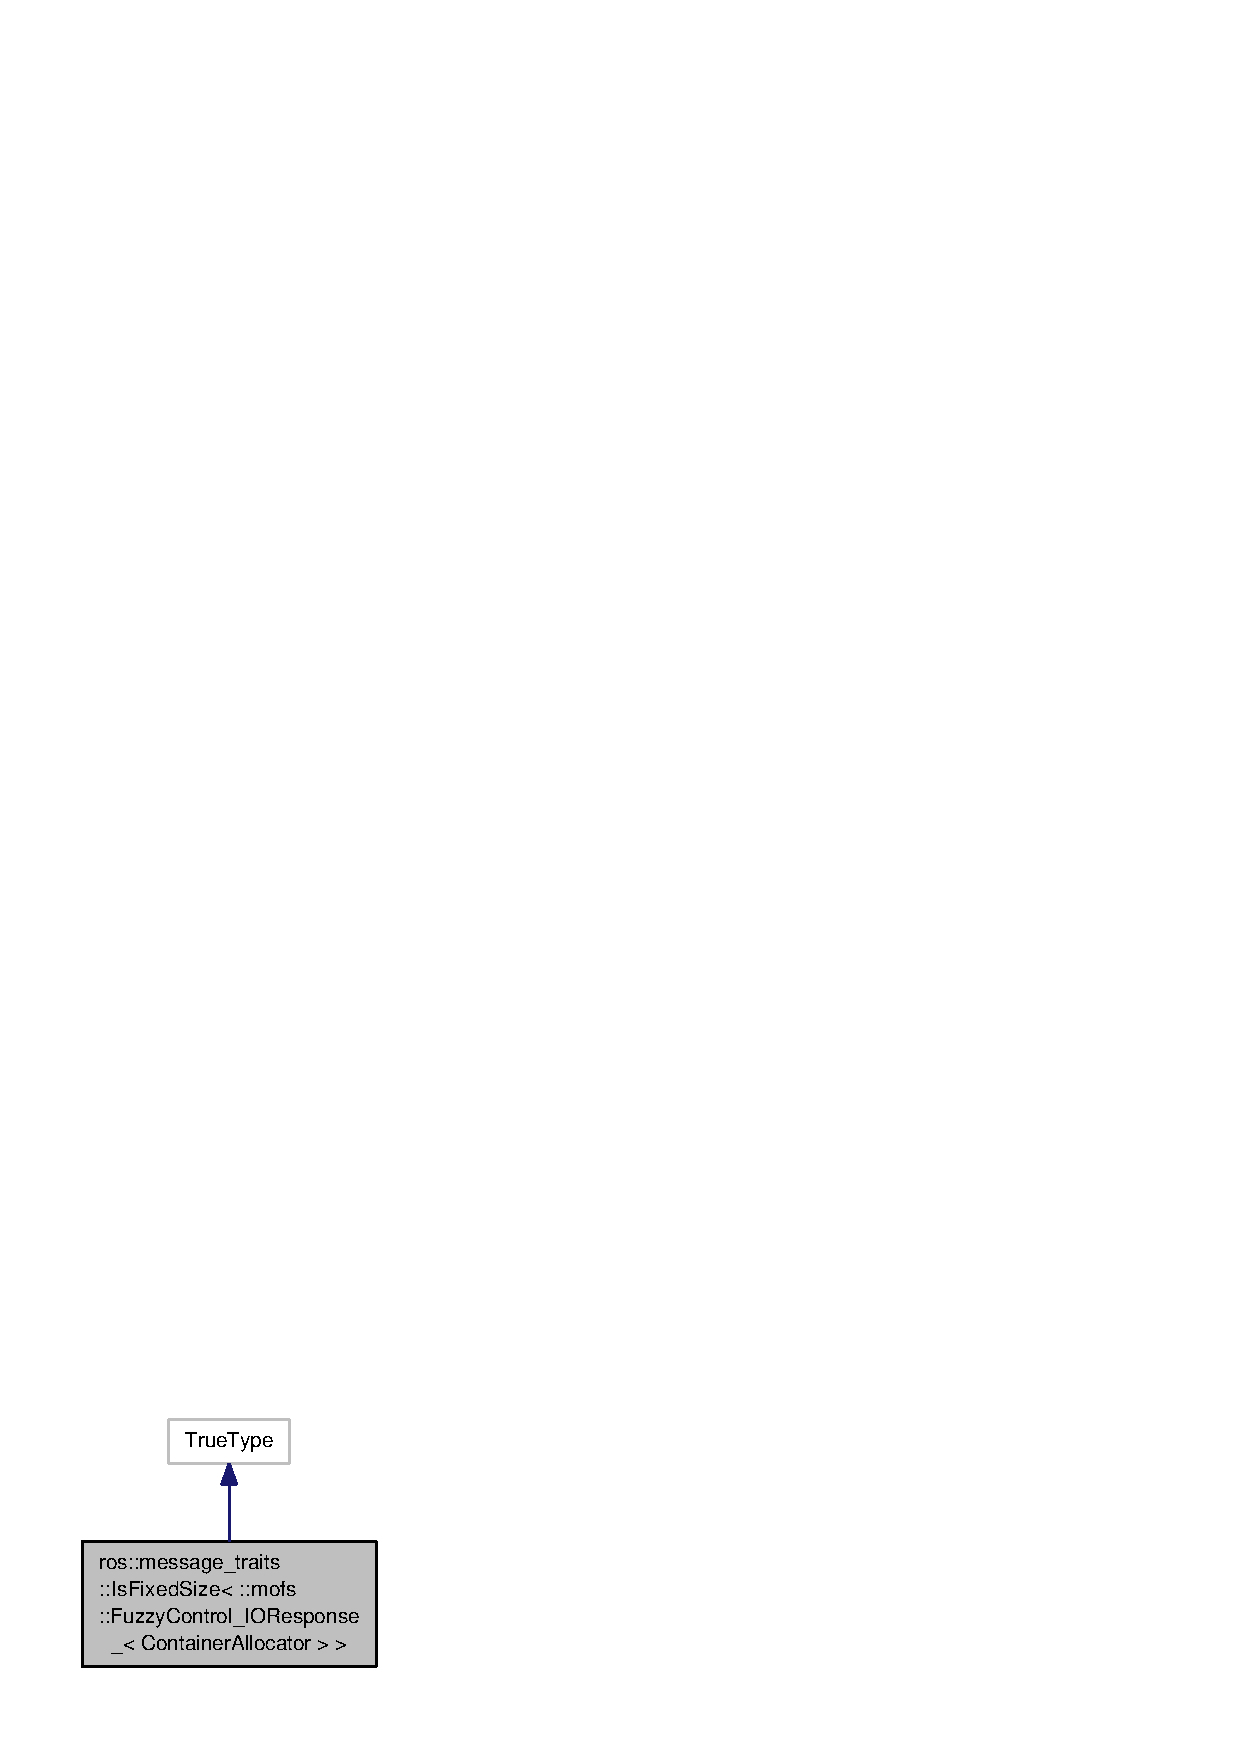
\includegraphics[width=184pt]{structros_1_1message__traits_1_1IsFixedSize_3_01_1_1mofs_1_1FuzzyControl__IOResponse___3_01Conta2977c3abc204ec51f4a3f03141ab7b07}
\end{center}
\end{figure}


\subsection{Detailed Description}
\subsubsection*{template$<$class Container\-Allocator$>$struct ros\-::message\-\_\-traits\-::\-Is\-Fixed\-Size$<$ \-::mofs\-::\-Fuzzy\-Control\-\_\-\-I\-O\-Response\-\_\-$<$ Container\-Allocator $>$ $>$}



Definition at line 181 of file Fuzzy\-Control\-\_\-\-I\-O.\-h.



The documentation for this struct was generated from the following file\-:\begin{DoxyCompactItemize}
\item 
{\bf Fuzzy\-Control\-\_\-\-I\-O.\-h}\end{DoxyCompactItemize}

\section{ros\-:\-:message\-\_\-traits\-:\-:Is\-Message$<$ \-:\-:mofs\-:\-:Fuzzy\-Control\-\_\-\-I\-O\-Request\-\_\-$<$ Container\-Allocator $>$ $>$ Struct Template Reference}
\label{structros_1_1message__traits_1_1IsMessage_3_01_1_1mofs_1_1FuzzyControl__IORequest___3_01ContainerAllocator_01_4_01_4}\index{ros\-::message\-\_\-traits\-::\-Is\-Message$<$ \-::mofs\-::\-Fuzzy\-Control\-\_\-\-I\-O\-Request\-\_\-$<$ Container\-Allocator $>$ $>$@{ros\-::message\-\_\-traits\-::\-Is\-Message$<$ \-::mofs\-::\-Fuzzy\-Control\-\_\-\-I\-O\-Request\-\_\-$<$ Container\-Allocator $>$ $>$}}


{\ttfamily \#include $<$Fuzzy\-Control\-\_\-\-I\-O.\-h$>$}



Inheritance diagram for ros\-:\-:message\-\_\-traits\-:\-:Is\-Message$<$ \-:\-:mofs\-:\-:Fuzzy\-Control\-\_\-\-I\-O\-Request\-\_\-$<$ Container\-Allocator $>$ $>$\-:\nopagebreak
\begin{figure}[H]
\begin{center}
\leavevmode
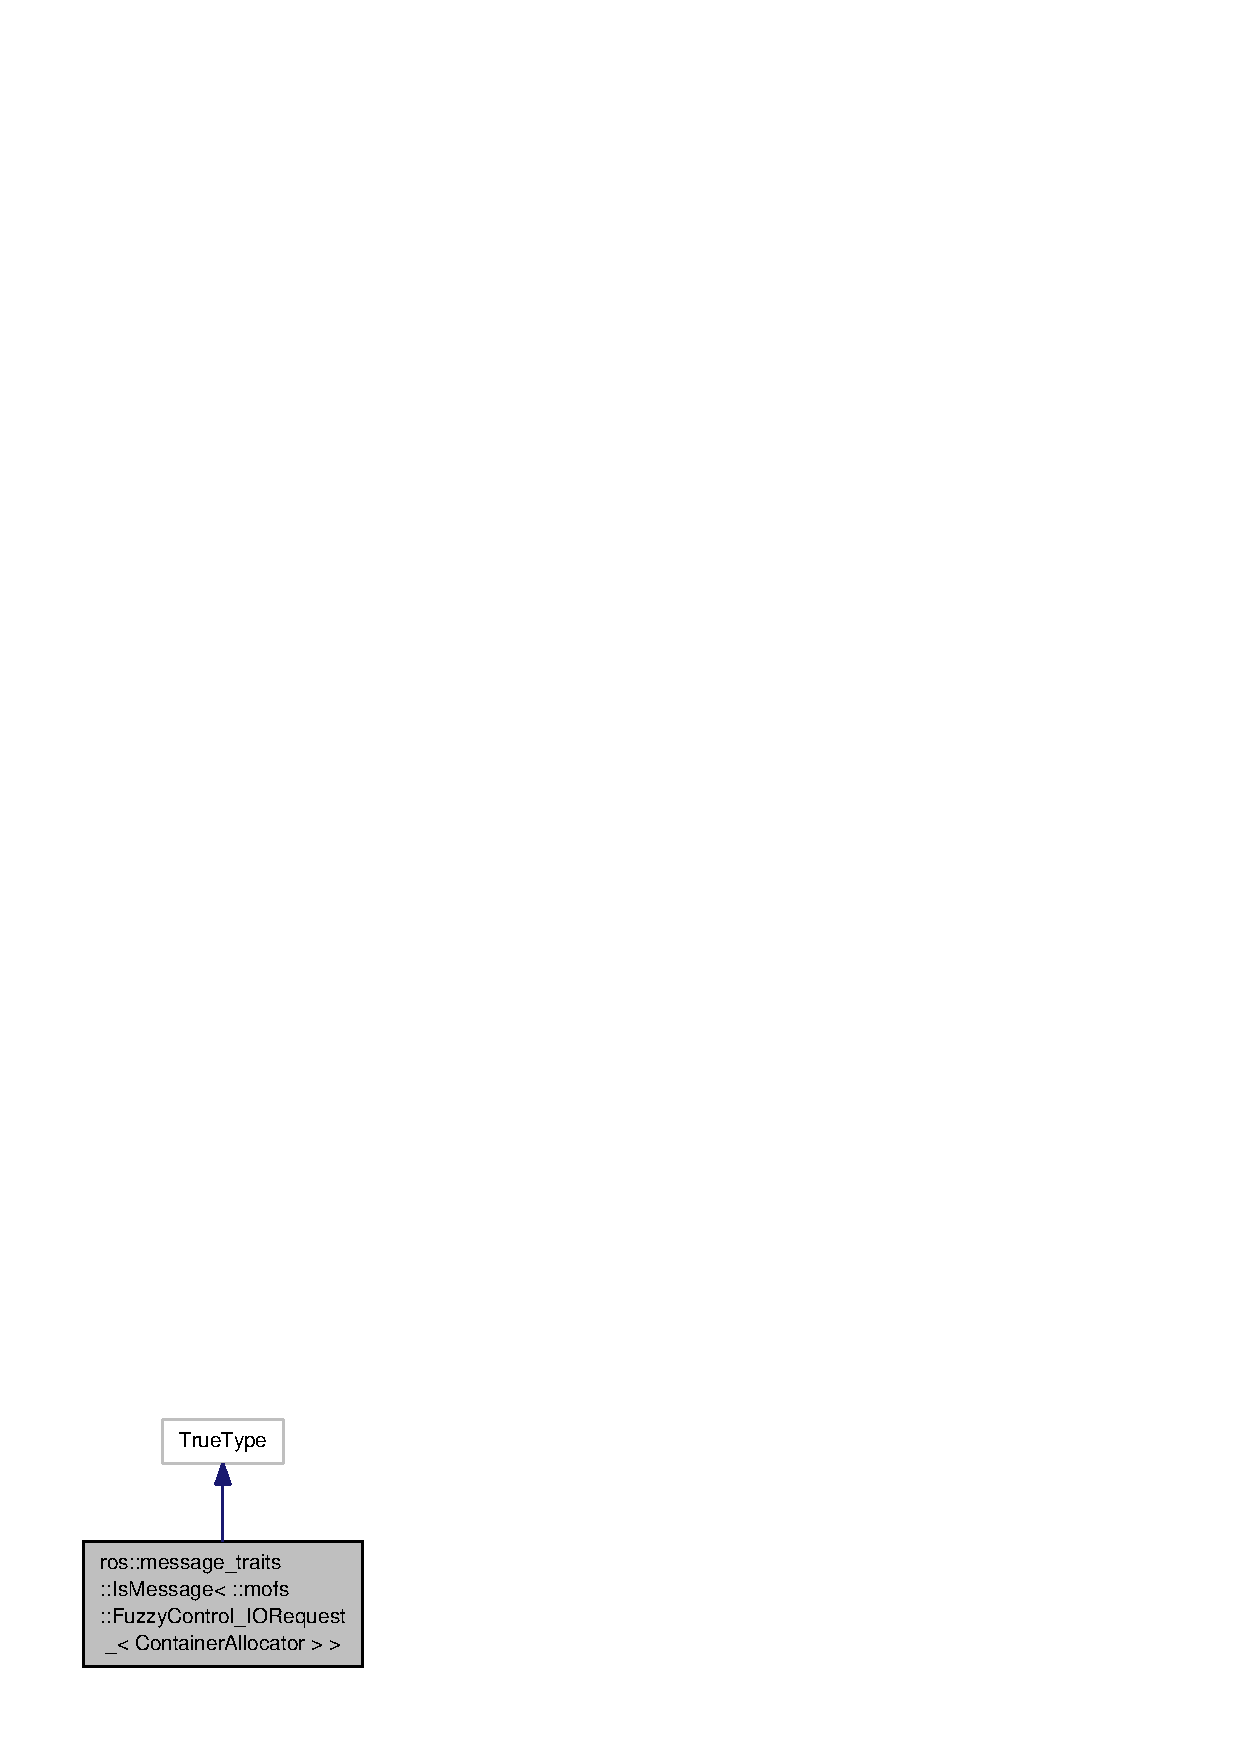
\includegraphics[width=178pt]{structros_1_1message__traits_1_1IsMessage_3_01_1_1mofs_1_1FuzzyControl__IORequest___3_01Containe93a612a5445d01ed4471ff069115dab0}
\end{center}
\end{figure}


\subsection{Detailed Description}
\subsubsection*{template$<$class Container\-Allocator$>$struct ros\-::message\-\_\-traits\-::\-Is\-Message$<$ \-::mofs\-::\-Fuzzy\-Control\-\_\-\-I\-O\-Request\-\_\-$<$ Container\-Allocator $>$ $>$}



Definition at line 98 of file Fuzzy\-Control\-\_\-\-I\-O.\-h.



The documentation for this struct was generated from the following file\-:\begin{DoxyCompactItemize}
\item 
{\bf Fuzzy\-Control\-\_\-\-I\-O.\-h}\end{DoxyCompactItemize}

\section{ros\-:\-:message\-\_\-traits\-:\-:Is\-Message$<$ \-:\-:mofs\-:\-:Fuzzy\-Control\-\_\-\-I\-O\-Request\-\_\-$<$ Container\-Allocator $>$const $>$ Struct Template Reference}
\label{structros_1_1message__traits_1_1IsMessage_3_01_1_1mofs_1_1FuzzyControl__IORequest___3_01ContainerAllocator_01_4const_01_01_4}\index{ros\-::message\-\_\-traits\-::\-Is\-Message$<$ \-::mofs\-::\-Fuzzy\-Control\-\_\-\-I\-O\-Request\-\_\-$<$ Container\-Allocator $>$const  $>$@{ros\-::message\-\_\-traits\-::\-Is\-Message$<$ \-::mofs\-::\-Fuzzy\-Control\-\_\-\-I\-O\-Request\-\_\-$<$ Container\-Allocator $>$const  $>$}}


{\ttfamily \#include $<$Fuzzy\-Control\-\_\-\-I\-O.\-h$>$}



Inheritance diagram for ros\-:\-:message\-\_\-traits\-:\-:Is\-Message$<$ \-:\-:mofs\-:\-:Fuzzy\-Control\-\_\-\-I\-O\-Request\-\_\-$<$ Container\-Allocator $>$const $>$\-:\nopagebreak
\begin{figure}[H]
\begin{center}
\leavevmode
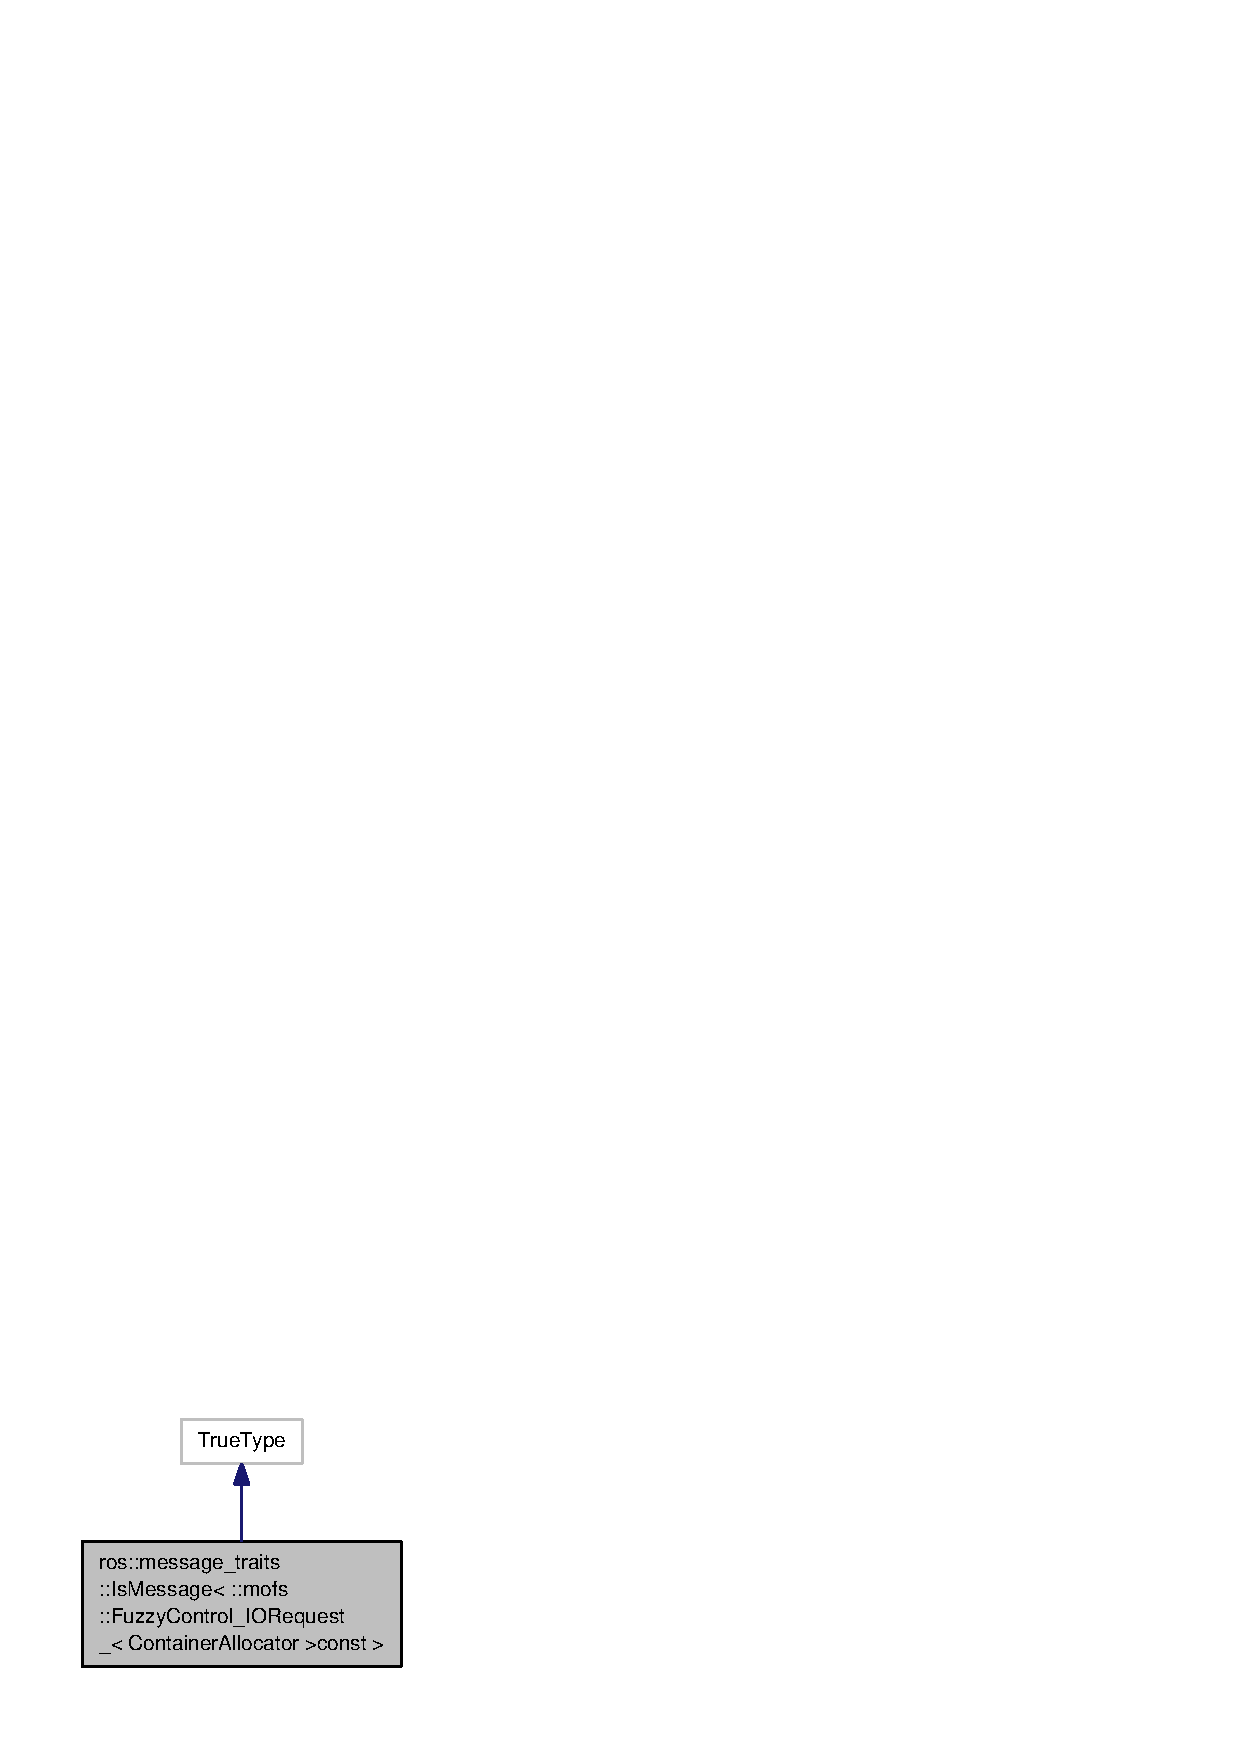
\includegraphics[width=196pt]{structros_1_1message__traits_1_1IsMessage_3_01_1_1mofs_1_1FuzzyControl__IORequest___3_01Containec24dc931b5d99c5d10052a522a7640b1}
\end{center}
\end{figure}


\subsection{Detailed Description}
\subsubsection*{template$<$class Container\-Allocator$>$struct ros\-::message\-\_\-traits\-::\-Is\-Message$<$ \-::mofs\-::\-Fuzzy\-Control\-\_\-\-I\-O\-Request\-\_\-$<$ Container\-Allocator $>$const  $>$}



Definition at line 99 of file Fuzzy\-Control\-\_\-\-I\-O.\-h.



The documentation for this struct was generated from the following file\-:\begin{DoxyCompactItemize}
\item 
{\bf Fuzzy\-Control\-\_\-\-I\-O.\-h}\end{DoxyCompactItemize}

\section{ros\-:\-:message\-\_\-traits\-:\-:Is\-Message$<$ \-:\-:mofs\-:\-:Fuzzy\-Control\-\_\-\-I\-O\-Response\-\_\-$<$ Container\-Allocator $>$ $>$ Struct Template Reference}
\label{structros_1_1message__traits_1_1IsMessage_3_01_1_1mofs_1_1FuzzyControl__IOResponse___3_01ContainerAllocator_01_4_01_4}\index{ros\-::message\-\_\-traits\-::\-Is\-Message$<$ \-::mofs\-::\-Fuzzy\-Control\-\_\-\-I\-O\-Response\-\_\-$<$ Container\-Allocator $>$ $>$@{ros\-::message\-\_\-traits\-::\-Is\-Message$<$ \-::mofs\-::\-Fuzzy\-Control\-\_\-\-I\-O\-Response\-\_\-$<$ Container\-Allocator $>$ $>$}}


{\ttfamily \#include $<$Fuzzy\-Control\-\_\-\-I\-O.\-h$>$}



Inheritance diagram for ros\-:\-:message\-\_\-traits\-:\-:Is\-Message$<$ \-:\-:mofs\-:\-:Fuzzy\-Control\-\_\-\-I\-O\-Response\-\_\-$<$ Container\-Allocator $>$ $>$\-:\nopagebreak
\begin{figure}[H]
\begin{center}
\leavevmode
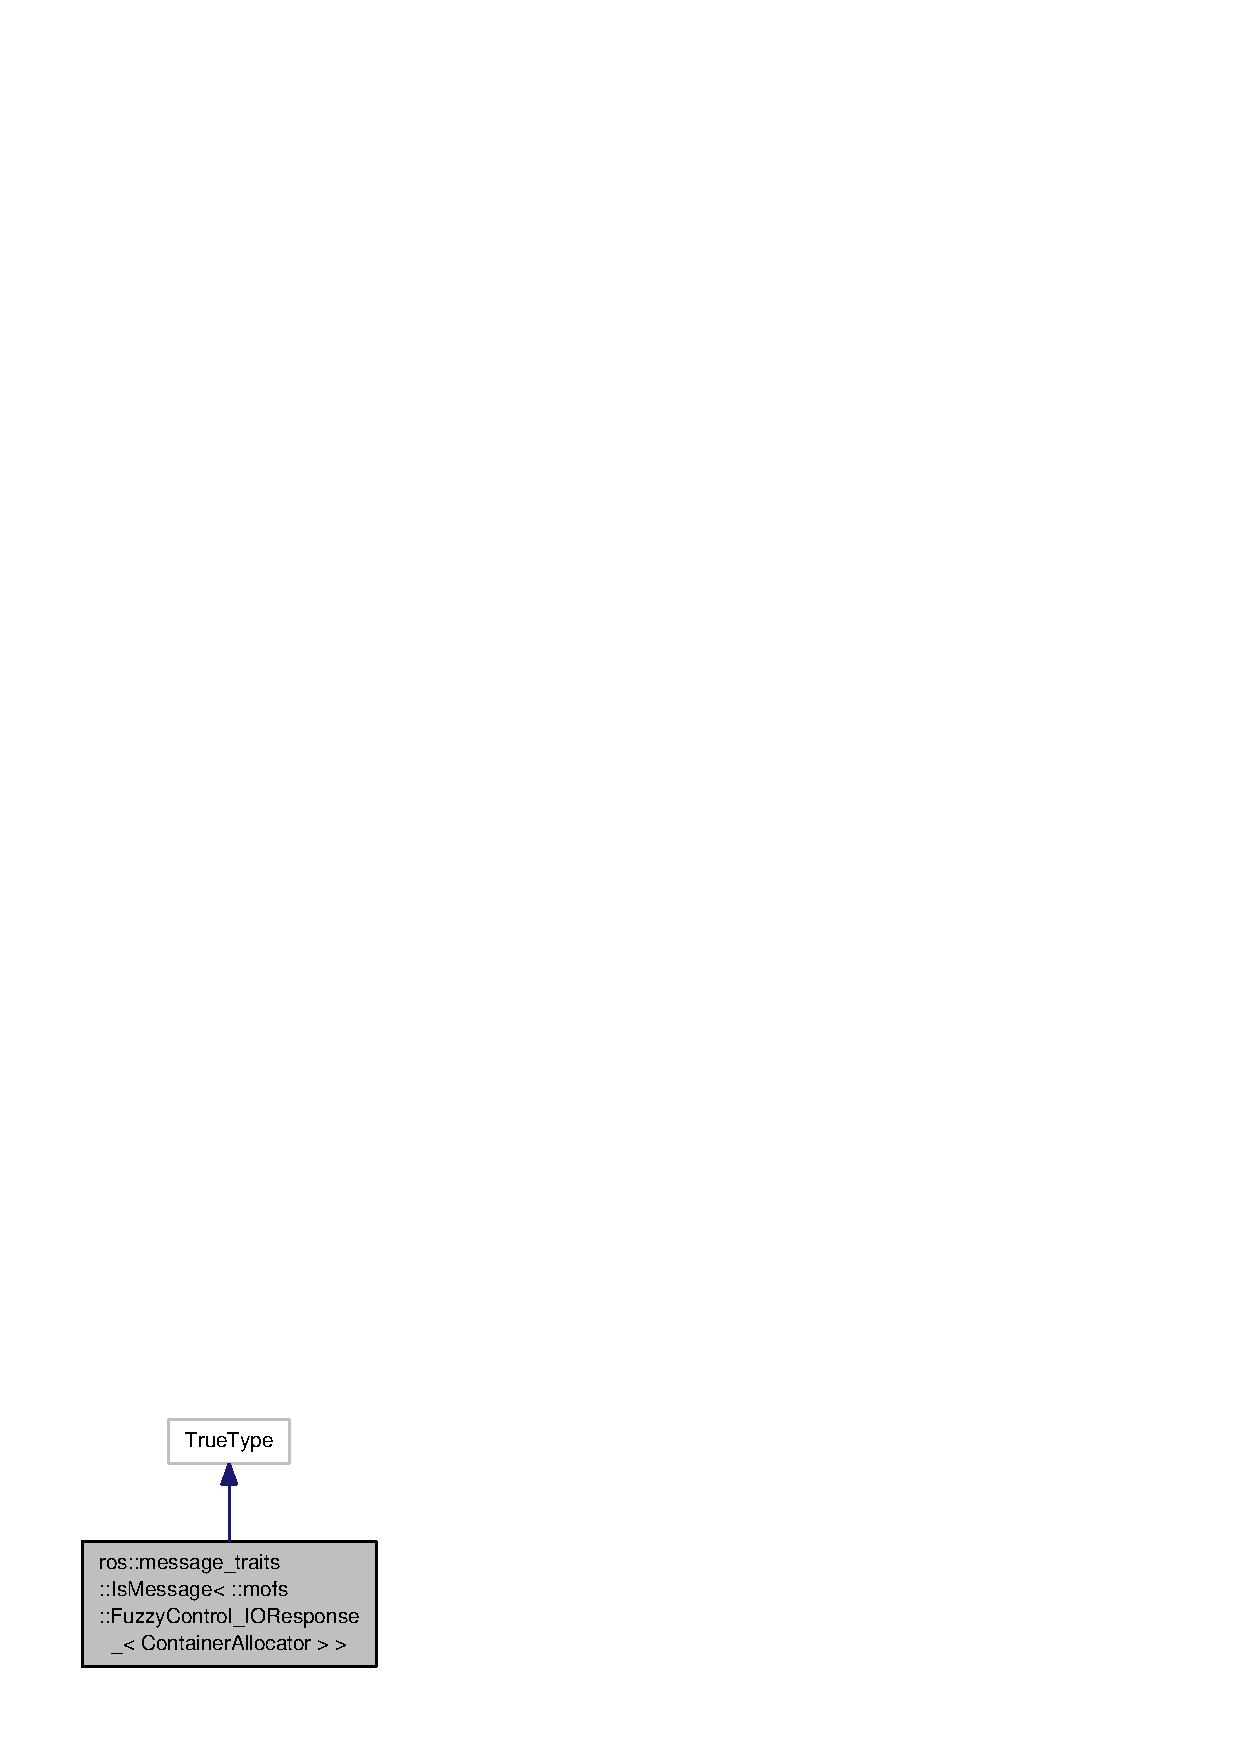
\includegraphics[width=184pt]{structros_1_1message__traits_1_1IsMessage_3_01_1_1mofs_1_1FuzzyControl__IOResponse___3_01Contain6dbf4ba7df2b6356a152c4fff661a9b8}
\end{center}
\end{figure}


\subsection{Detailed Description}
\subsubsection*{template$<$class Container\-Allocator$>$struct ros\-::message\-\_\-traits\-::\-Is\-Message$<$ \-::mofs\-::\-Fuzzy\-Control\-\_\-\-I\-O\-Response\-\_\-$<$ Container\-Allocator $>$ $>$}



Definition at line 144 of file Fuzzy\-Control\-\_\-\-I\-O.\-h.



The documentation for this struct was generated from the following file\-:\begin{DoxyCompactItemize}
\item 
{\bf Fuzzy\-Control\-\_\-\-I\-O.\-h}\end{DoxyCompactItemize}

\section{ros\-:\-:message\-\_\-traits\-:\-:Is\-Message$<$ \-:\-:mofs\-:\-:Fuzzy\-Control\-\_\-\-I\-O\-Response\-\_\-$<$ Container\-Allocator $>$const $>$ Struct Template Reference}
\label{structros_1_1message__traits_1_1IsMessage_3_01_1_1mofs_1_1FuzzyControl__IOResponse___3_01ContainerAllocator_01_4const_01_01_4}\index{ros\-::message\-\_\-traits\-::\-Is\-Message$<$ \-::mofs\-::\-Fuzzy\-Control\-\_\-\-I\-O\-Response\-\_\-$<$ Container\-Allocator $>$const  $>$@{ros\-::message\-\_\-traits\-::\-Is\-Message$<$ \-::mofs\-::\-Fuzzy\-Control\-\_\-\-I\-O\-Response\-\_\-$<$ Container\-Allocator $>$const  $>$}}


{\ttfamily \#include $<$Fuzzy\-Control\-\_\-\-I\-O.\-h$>$}



Inheritance diagram for ros\-:\-:message\-\_\-traits\-:\-:Is\-Message$<$ \-:\-:mofs\-:\-:Fuzzy\-Control\-\_\-\-I\-O\-Response\-\_\-$<$ Container\-Allocator $>$const $>$\-:\nopagebreak
\begin{figure}[H]
\begin{center}
\leavevmode
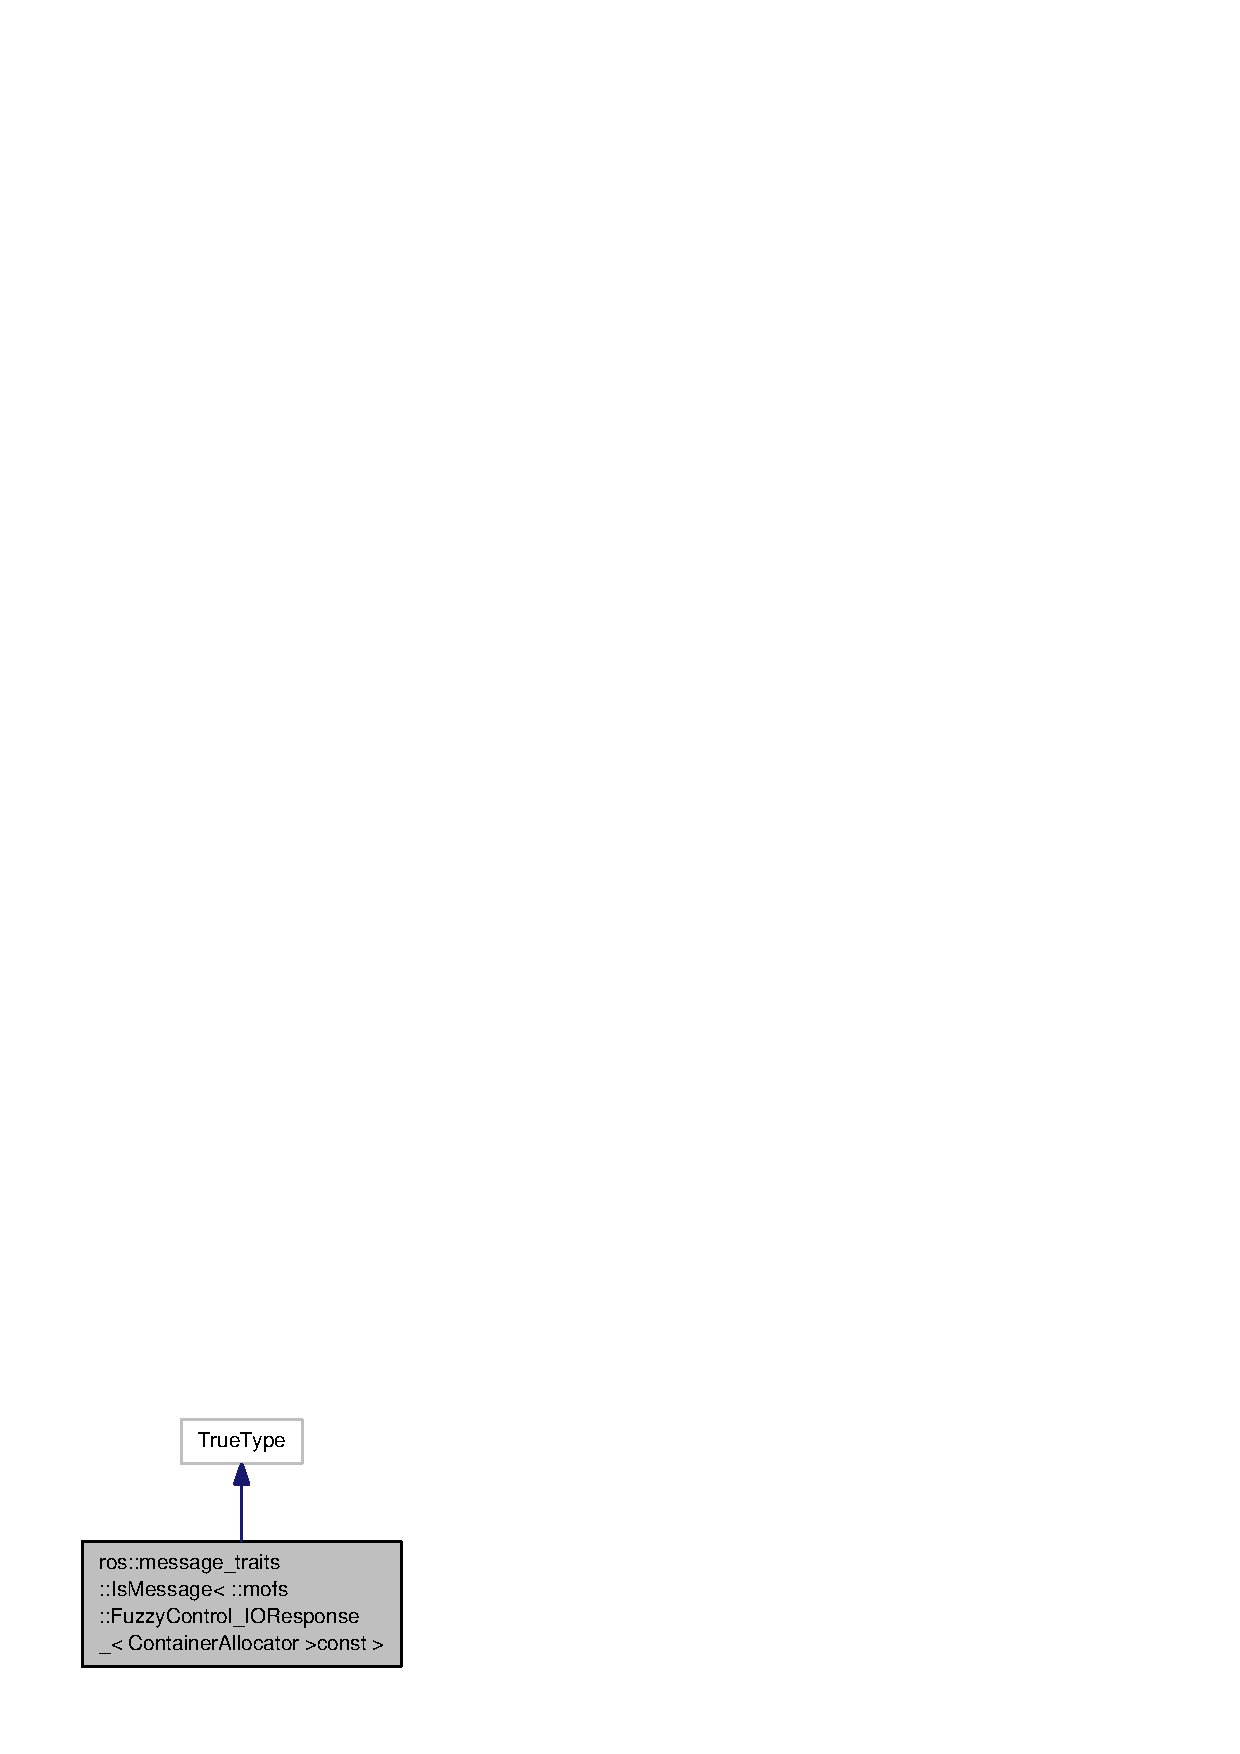
\includegraphics[width=196pt]{structros_1_1message__traits_1_1IsMessage_3_01_1_1mofs_1_1FuzzyControl__IOResponse___3_01Contain8f713a70a01aa5e3c9f892c201a7a429}
\end{center}
\end{figure}


\subsection{Detailed Description}
\subsubsection*{template$<$class Container\-Allocator$>$struct ros\-::message\-\_\-traits\-::\-Is\-Message$<$ \-::mofs\-::\-Fuzzy\-Control\-\_\-\-I\-O\-Response\-\_\-$<$ Container\-Allocator $>$const  $>$}



Definition at line 145 of file Fuzzy\-Control\-\_\-\-I\-O.\-h.



The documentation for this struct was generated from the following file\-:\begin{DoxyCompactItemize}
\item 
{\bf Fuzzy\-Control\-\_\-\-I\-O.\-h}\end{DoxyCompactItemize}

\section{ros\-:\-:message\-\_\-traits\-:\-:M\-D5\-Sum$<$ \-:\-:mofs\-:\-:Fuzzy\-Control\-\_\-\-I\-O\-Request\-\_\-$<$ Container\-Allocator $>$ $>$ Struct Template Reference}
\label{structros_1_1message__traits_1_1MD5Sum_3_01_1_1mofs_1_1FuzzyControl__IORequest___3_01ContainerAllocator_01_4_01_4}\index{ros\-::message\-\_\-traits\-::\-M\-D5\-Sum$<$ \-::mofs\-::\-Fuzzy\-Control\-\_\-\-I\-O\-Request\-\_\-$<$ Container\-Allocator $>$ $>$@{ros\-::message\-\_\-traits\-::\-M\-D5\-Sum$<$ \-::mofs\-::\-Fuzzy\-Control\-\_\-\-I\-O\-Request\-\_\-$<$ Container\-Allocator $>$ $>$}}


{\ttfamily \#include $<$Fuzzy\-Control\-\_\-\-I\-O.\-h$>$}

\subsection*{Static Public Member Functions}
\begin{DoxyCompactItemize}
\item 
static const char $\ast$ {\bf value} ()
\item 
static const char $\ast$ {\bf value} (const \-::{\bf mofs\-::\-Fuzzy\-Control\-\_\-\-I\-O\-Request\-\_\-}$<$ Container\-Allocator $>$ \&)
\end{DoxyCompactItemize}
\subsection*{Static Public Attributes}
\begin{DoxyCompactItemize}
\item 
static const uint64\-\_\-t {\bf static\-\_\-value1} = 0xea0b038bccdff67b\-U\-L\-L
\item 
static const uint64\-\_\-t {\bf static\-\_\-value2} = 0xc1751623cde4aed3\-U\-L\-L
\end{DoxyCompactItemize}


\subsection{Detailed Description}
\subsubsection*{template$<$class Container\-Allocator$>$struct ros\-::message\-\_\-traits\-::\-M\-D5\-Sum$<$ \-::mofs\-::\-Fuzzy\-Control\-\_\-\-I\-O\-Request\-\_\-$<$ Container\-Allocator $>$ $>$}



Definition at line 101 of file Fuzzy\-Control\-\_\-\-I\-O.\-h.



\subsection{Member Function Documentation}
\index{ros\-::message\-\_\-traits\-::\-M\-D5\-Sum$<$ \-::mofs\-::\-Fuzzy\-Control\-\_\-\-I\-O\-Request\-\_\-$<$ Container\-Allocator $>$ $>$@{ros\-::message\-\_\-traits\-::\-M\-D5\-Sum$<$ \-::mofs\-::\-Fuzzy\-Control\-\_\-\-I\-O\-Request\-\_\-$<$ Container\-Allocator $>$ $>$}!value@{value}}
\index{value@{value}!ros::message_traits::MD5Sum< ::mofs::FuzzyControl_IORequest_< ContainerAllocator > >@{ros\-::message\-\_\-traits\-::\-M\-D5\-Sum$<$ \-::mofs\-::\-Fuzzy\-Control\-\_\-\-I\-O\-Request\-\_\-$<$ Container\-Allocator $>$ $>$}}
\subsubsection[{value}]{\setlength{\rightskip}{0pt plus 5cm}template$<$class Container\-Allocator $>$ static const char$\ast$ ros\-::message\-\_\-traits\-::\-M\-D5\-Sum$<$ \-::{\bf mofs\-::\-Fuzzy\-Control\-\_\-\-I\-O\-Request\-\_\-}$<$ Container\-Allocator $>$ $>$\-::value (
\begin{DoxyParamCaption}
{}
\end{DoxyParamCaption}
)\hspace{0.3cm}{\ttfamily [inline]}, {\ttfamily [static]}}\label{structros_1_1message__traits_1_1MD5Sum_3_01_1_1mofs_1_1FuzzyControl__IORequest___3_01ContainerAllocator_01_4_01_4_a0664c11a8f328ab886c12a7d5e946010}


Definition at line 102 of file Fuzzy\-Control\-\_\-\-I\-O.\-h.

\index{ros\-::message\-\_\-traits\-::\-M\-D5\-Sum$<$ \-::mofs\-::\-Fuzzy\-Control\-\_\-\-I\-O\-Request\-\_\-$<$ Container\-Allocator $>$ $>$@{ros\-::message\-\_\-traits\-::\-M\-D5\-Sum$<$ \-::mofs\-::\-Fuzzy\-Control\-\_\-\-I\-O\-Request\-\_\-$<$ Container\-Allocator $>$ $>$}!value@{value}}
\index{value@{value}!ros::message_traits::MD5Sum< ::mofs::FuzzyControl_IORequest_< ContainerAllocator > >@{ros\-::message\-\_\-traits\-::\-M\-D5\-Sum$<$ \-::mofs\-::\-Fuzzy\-Control\-\_\-\-I\-O\-Request\-\_\-$<$ Container\-Allocator $>$ $>$}}
\subsubsection[{value}]{\setlength{\rightskip}{0pt plus 5cm}template$<$class Container\-Allocator $>$ static const char$\ast$ ros\-::message\-\_\-traits\-::\-M\-D5\-Sum$<$ \-::{\bf mofs\-::\-Fuzzy\-Control\-\_\-\-I\-O\-Request\-\_\-}$<$ Container\-Allocator $>$ $>$\-::value (
\begin{DoxyParamCaption}
\item[{const \-::{\bf mofs\-::\-Fuzzy\-Control\-\_\-\-I\-O\-Request\-\_\-}$<$ Container\-Allocator $>$ \&}]{}
\end{DoxyParamCaption}
)\hspace{0.3cm}{\ttfamily [inline]}, {\ttfamily [static]}}\label{structros_1_1message__traits_1_1MD5Sum_3_01_1_1mofs_1_1FuzzyControl__IORequest___3_01ContainerAllocator_01_4_01_4_a18e7b94f676b75fc9b049a9a370e48f7}


Definition at line 107 of file Fuzzy\-Control\-\_\-\-I\-O.\-h.



\subsection{Member Data Documentation}
\index{ros\-::message\-\_\-traits\-::\-M\-D5\-Sum$<$ \-::mofs\-::\-Fuzzy\-Control\-\_\-\-I\-O\-Request\-\_\-$<$ Container\-Allocator $>$ $>$@{ros\-::message\-\_\-traits\-::\-M\-D5\-Sum$<$ \-::mofs\-::\-Fuzzy\-Control\-\_\-\-I\-O\-Request\-\_\-$<$ Container\-Allocator $>$ $>$}!static\-\_\-value1@{static\-\_\-value1}}
\index{static\-\_\-value1@{static\-\_\-value1}!ros::message_traits::MD5Sum< ::mofs::FuzzyControl_IORequest_< ContainerAllocator > >@{ros\-::message\-\_\-traits\-::\-M\-D5\-Sum$<$ \-::mofs\-::\-Fuzzy\-Control\-\_\-\-I\-O\-Request\-\_\-$<$ Container\-Allocator $>$ $>$}}
\subsubsection[{static\-\_\-value1}]{\setlength{\rightskip}{0pt plus 5cm}template$<$class Container\-Allocator $>$ const uint64\-\_\-t ros\-::message\-\_\-traits\-::\-M\-D5\-Sum$<$ \-::{\bf mofs\-::\-Fuzzy\-Control\-\_\-\-I\-O\-Request\-\_\-}$<$ Container\-Allocator $>$ $>$\-::static\-\_\-value1 = 0xea0b038bccdff67b\-U\-L\-L\hspace{0.3cm}{\ttfamily [static]}}\label{structros_1_1message__traits_1_1MD5Sum_3_01_1_1mofs_1_1FuzzyControl__IORequest___3_01ContainerAllocator_01_4_01_4_a27fadbc427f38eb0f39089c866cc4a00}


Definition at line 108 of file Fuzzy\-Control\-\_\-\-I\-O.\-h.

\index{ros\-::message\-\_\-traits\-::\-M\-D5\-Sum$<$ \-::mofs\-::\-Fuzzy\-Control\-\_\-\-I\-O\-Request\-\_\-$<$ Container\-Allocator $>$ $>$@{ros\-::message\-\_\-traits\-::\-M\-D5\-Sum$<$ \-::mofs\-::\-Fuzzy\-Control\-\_\-\-I\-O\-Request\-\_\-$<$ Container\-Allocator $>$ $>$}!static\-\_\-value2@{static\-\_\-value2}}
\index{static\-\_\-value2@{static\-\_\-value2}!ros::message_traits::MD5Sum< ::mofs::FuzzyControl_IORequest_< ContainerAllocator > >@{ros\-::message\-\_\-traits\-::\-M\-D5\-Sum$<$ \-::mofs\-::\-Fuzzy\-Control\-\_\-\-I\-O\-Request\-\_\-$<$ Container\-Allocator $>$ $>$}}
\subsubsection[{static\-\_\-value2}]{\setlength{\rightskip}{0pt plus 5cm}template$<$class Container\-Allocator $>$ const uint64\-\_\-t ros\-::message\-\_\-traits\-::\-M\-D5\-Sum$<$ \-::{\bf mofs\-::\-Fuzzy\-Control\-\_\-\-I\-O\-Request\-\_\-}$<$ Container\-Allocator $>$ $>$\-::static\-\_\-value2 = 0xc1751623cde4aed3\-U\-L\-L\hspace{0.3cm}{\ttfamily [static]}}\label{structros_1_1message__traits_1_1MD5Sum_3_01_1_1mofs_1_1FuzzyControl__IORequest___3_01ContainerAllocator_01_4_01_4_a5c4770328e0f92ac5bd8fb068fa716d4}


Definition at line 109 of file Fuzzy\-Control\-\_\-\-I\-O.\-h.



The documentation for this struct was generated from the following file\-:\begin{DoxyCompactItemize}
\item 
{\bf Fuzzy\-Control\-\_\-\-I\-O.\-h}\end{DoxyCompactItemize}

\section{ros\-:\-:message\-\_\-traits\-:\-:M\-D5\-Sum$<$ \-:\-:mofs\-:\-:Fuzzy\-Control\-\_\-\-I\-O\-Response\-\_\-$<$ Container\-Allocator $>$ $>$ Struct Template Reference}
\label{structros_1_1message__traits_1_1MD5Sum_3_01_1_1mofs_1_1FuzzyControl__IOResponse___3_01ContainerAllocator_01_4_01_4}\index{ros\-::message\-\_\-traits\-::\-M\-D5\-Sum$<$ \-::mofs\-::\-Fuzzy\-Control\-\_\-\-I\-O\-Response\-\_\-$<$ Container\-Allocator $>$ $>$@{ros\-::message\-\_\-traits\-::\-M\-D5\-Sum$<$ \-::mofs\-::\-Fuzzy\-Control\-\_\-\-I\-O\-Response\-\_\-$<$ Container\-Allocator $>$ $>$}}


{\ttfamily \#include $<$Fuzzy\-Control\-\_\-\-I\-O.\-h$>$}

\subsection*{Static Public Member Functions}
\begin{DoxyCompactItemize}
\item 
static const char $\ast$ {\bf value} ()
\item 
static const char $\ast$ {\bf value} (const \-::{\bf mofs\-::\-Fuzzy\-Control\-\_\-\-I\-O\-Response\-\_\-}$<$ Container\-Allocator $>$ \&)
\end{DoxyCompactItemize}
\subsection*{Static Public Attributes}
\begin{DoxyCompactItemize}
\item 
static const uint64\-\_\-t {\bf static\-\_\-value1} = 0xdc04e8385a5c2f79\-U\-L\-L
\item 
static const uint64\-\_\-t {\bf static\-\_\-value2} = 0x2e8299232db8e2eb\-U\-L\-L
\end{DoxyCompactItemize}


\subsection{Detailed Description}
\subsubsection*{template$<$class Container\-Allocator$>$struct ros\-::message\-\_\-traits\-::\-M\-D5\-Sum$<$ \-::mofs\-::\-Fuzzy\-Control\-\_\-\-I\-O\-Response\-\_\-$<$ Container\-Allocator $>$ $>$}



Definition at line 147 of file Fuzzy\-Control\-\_\-\-I\-O.\-h.



\subsection{Member Function Documentation}
\index{ros\-::message\-\_\-traits\-::\-M\-D5\-Sum$<$ \-::mofs\-::\-Fuzzy\-Control\-\_\-\-I\-O\-Response\-\_\-$<$ Container\-Allocator $>$ $>$@{ros\-::message\-\_\-traits\-::\-M\-D5\-Sum$<$ \-::mofs\-::\-Fuzzy\-Control\-\_\-\-I\-O\-Response\-\_\-$<$ Container\-Allocator $>$ $>$}!value@{value}}
\index{value@{value}!ros::message_traits::MD5Sum< ::mofs::FuzzyControl_IOResponse_< ContainerAllocator > >@{ros\-::message\-\_\-traits\-::\-M\-D5\-Sum$<$ \-::mofs\-::\-Fuzzy\-Control\-\_\-\-I\-O\-Response\-\_\-$<$ Container\-Allocator $>$ $>$}}
\subsubsection[{value}]{\setlength{\rightskip}{0pt plus 5cm}template$<$class Container\-Allocator $>$ static const char$\ast$ ros\-::message\-\_\-traits\-::\-M\-D5\-Sum$<$ \-::{\bf mofs\-::\-Fuzzy\-Control\-\_\-\-I\-O\-Response\-\_\-}$<$ Container\-Allocator $>$ $>$\-::value (
\begin{DoxyParamCaption}
{}
\end{DoxyParamCaption}
)\hspace{0.3cm}{\ttfamily [inline]}, {\ttfamily [static]}}\label{structros_1_1message__traits_1_1MD5Sum_3_01_1_1mofs_1_1FuzzyControl__IOResponse___3_01ContainerAllocator_01_4_01_4_ab95b8eaefa55bbc18778e33d0b4fb6a0}


Definition at line 148 of file Fuzzy\-Control\-\_\-\-I\-O.\-h.

\index{ros\-::message\-\_\-traits\-::\-M\-D5\-Sum$<$ \-::mofs\-::\-Fuzzy\-Control\-\_\-\-I\-O\-Response\-\_\-$<$ Container\-Allocator $>$ $>$@{ros\-::message\-\_\-traits\-::\-M\-D5\-Sum$<$ \-::mofs\-::\-Fuzzy\-Control\-\_\-\-I\-O\-Response\-\_\-$<$ Container\-Allocator $>$ $>$}!value@{value}}
\index{value@{value}!ros::message_traits::MD5Sum< ::mofs::FuzzyControl_IOResponse_< ContainerAllocator > >@{ros\-::message\-\_\-traits\-::\-M\-D5\-Sum$<$ \-::mofs\-::\-Fuzzy\-Control\-\_\-\-I\-O\-Response\-\_\-$<$ Container\-Allocator $>$ $>$}}
\subsubsection[{value}]{\setlength{\rightskip}{0pt plus 5cm}template$<$class Container\-Allocator $>$ static const char$\ast$ ros\-::message\-\_\-traits\-::\-M\-D5\-Sum$<$ \-::{\bf mofs\-::\-Fuzzy\-Control\-\_\-\-I\-O\-Response\-\_\-}$<$ Container\-Allocator $>$ $>$\-::value (
\begin{DoxyParamCaption}
\item[{const \-::{\bf mofs\-::\-Fuzzy\-Control\-\_\-\-I\-O\-Response\-\_\-}$<$ Container\-Allocator $>$ \&}]{}
\end{DoxyParamCaption}
)\hspace{0.3cm}{\ttfamily [inline]}, {\ttfamily [static]}}\label{structros_1_1message__traits_1_1MD5Sum_3_01_1_1mofs_1_1FuzzyControl__IOResponse___3_01ContainerAllocator_01_4_01_4_a8778132fbf9de414ca8629426176ea3a}


Definition at line 153 of file Fuzzy\-Control\-\_\-\-I\-O.\-h.



\subsection{Member Data Documentation}
\index{ros\-::message\-\_\-traits\-::\-M\-D5\-Sum$<$ \-::mofs\-::\-Fuzzy\-Control\-\_\-\-I\-O\-Response\-\_\-$<$ Container\-Allocator $>$ $>$@{ros\-::message\-\_\-traits\-::\-M\-D5\-Sum$<$ \-::mofs\-::\-Fuzzy\-Control\-\_\-\-I\-O\-Response\-\_\-$<$ Container\-Allocator $>$ $>$}!static\-\_\-value1@{static\-\_\-value1}}
\index{static\-\_\-value1@{static\-\_\-value1}!ros::message_traits::MD5Sum< ::mofs::FuzzyControl_IOResponse_< ContainerAllocator > >@{ros\-::message\-\_\-traits\-::\-M\-D5\-Sum$<$ \-::mofs\-::\-Fuzzy\-Control\-\_\-\-I\-O\-Response\-\_\-$<$ Container\-Allocator $>$ $>$}}
\subsubsection[{static\-\_\-value1}]{\setlength{\rightskip}{0pt plus 5cm}template$<$class Container\-Allocator $>$ const uint64\-\_\-t ros\-::message\-\_\-traits\-::\-M\-D5\-Sum$<$ \-::{\bf mofs\-::\-Fuzzy\-Control\-\_\-\-I\-O\-Response\-\_\-}$<$ Container\-Allocator $>$ $>$\-::static\-\_\-value1 = 0xdc04e8385a5c2f79\-U\-L\-L\hspace{0.3cm}{\ttfamily [static]}}\label{structros_1_1message__traits_1_1MD5Sum_3_01_1_1mofs_1_1FuzzyControl__IOResponse___3_01ContainerAllocator_01_4_01_4_a0f72b8fabff26116d3be1c0f8aeecc3b}


Definition at line 154 of file Fuzzy\-Control\-\_\-\-I\-O.\-h.

\index{ros\-::message\-\_\-traits\-::\-M\-D5\-Sum$<$ \-::mofs\-::\-Fuzzy\-Control\-\_\-\-I\-O\-Response\-\_\-$<$ Container\-Allocator $>$ $>$@{ros\-::message\-\_\-traits\-::\-M\-D5\-Sum$<$ \-::mofs\-::\-Fuzzy\-Control\-\_\-\-I\-O\-Response\-\_\-$<$ Container\-Allocator $>$ $>$}!static\-\_\-value2@{static\-\_\-value2}}
\index{static\-\_\-value2@{static\-\_\-value2}!ros::message_traits::MD5Sum< ::mofs::FuzzyControl_IOResponse_< ContainerAllocator > >@{ros\-::message\-\_\-traits\-::\-M\-D5\-Sum$<$ \-::mofs\-::\-Fuzzy\-Control\-\_\-\-I\-O\-Response\-\_\-$<$ Container\-Allocator $>$ $>$}}
\subsubsection[{static\-\_\-value2}]{\setlength{\rightskip}{0pt plus 5cm}template$<$class Container\-Allocator $>$ const uint64\-\_\-t ros\-::message\-\_\-traits\-::\-M\-D5\-Sum$<$ \-::{\bf mofs\-::\-Fuzzy\-Control\-\_\-\-I\-O\-Response\-\_\-}$<$ Container\-Allocator $>$ $>$\-::static\-\_\-value2 = 0x2e8299232db8e2eb\-U\-L\-L\hspace{0.3cm}{\ttfamily [static]}}\label{structros_1_1message__traits_1_1MD5Sum_3_01_1_1mofs_1_1FuzzyControl__IOResponse___3_01ContainerAllocator_01_4_01_4_a3d39b14f02ad2136f388a81eb466b897}


Definition at line 155 of file Fuzzy\-Control\-\_\-\-I\-O.\-h.



The documentation for this struct was generated from the following file\-:\begin{DoxyCompactItemize}
\item 
{\bf Fuzzy\-Control\-\_\-\-I\-O.\-h}\end{DoxyCompactItemize}

\section{ros\-:\-:service\-\_\-traits\-:\-:M\-D5\-Sum$<$ mofs\-:\-:Fuzzy\-Control\-\_\-\-I\-O $>$ Struct Template Reference}
\label{structros_1_1service__traits_1_1MD5Sum_3_01mofs_1_1FuzzyControl__IO_01_4}\index{ros\-::service\-\_\-traits\-::\-M\-D5\-Sum$<$ mofs\-::\-Fuzzy\-Control\-\_\-\-I\-O $>$@{ros\-::service\-\_\-traits\-::\-M\-D5\-Sum$<$ mofs\-::\-Fuzzy\-Control\-\_\-\-I\-O $>$}}


{\ttfamily \#include $<$Fuzzy\-Control\-\_\-\-I\-O.\-h$>$}

\subsection*{Static Public Member Functions}
\begin{DoxyCompactItemize}
\item 
static const char $\ast$ {\bf value} ()
\item 
static const char $\ast$ {\bf value} (const {\bf mofs\-::\-Fuzzy\-Control\-\_\-\-I\-O} \&)
\end{DoxyCompactItemize}


\subsection{Detailed Description}
\subsubsection*{template$<$$>$struct ros\-::service\-\_\-traits\-::\-M\-D5\-Sum$<$ mofs\-::\-Fuzzy\-Control\-\_\-\-I\-O $>$}



Definition at line 225 of file Fuzzy\-Control\-\_\-\-I\-O.\-h.



\subsection{Member Function Documentation}
\index{ros\-::service\-\_\-traits\-::\-M\-D5\-Sum$<$ mofs\-::\-Fuzzy\-Control\-\_\-\-I\-O $>$@{ros\-::service\-\_\-traits\-::\-M\-D5\-Sum$<$ mofs\-::\-Fuzzy\-Control\-\_\-\-I\-O $>$}!value@{value}}
\index{value@{value}!ros::service_traits::MD5Sum< mofs::FuzzyControl_IO >@{ros\-::service\-\_\-traits\-::\-M\-D5\-Sum$<$ mofs\-::\-Fuzzy\-Control\-\_\-\-I\-O $>$}}
\subsubsection[{value}]{\setlength{\rightskip}{0pt plus 5cm}static const char$\ast$ ros\-::service\-\_\-traits\-::\-M\-D5\-Sum$<$ {\bf mofs\-::\-Fuzzy\-Control\-\_\-\-I\-O} $>$\-::value (
\begin{DoxyParamCaption}
{}
\end{DoxyParamCaption}
)\hspace{0.3cm}{\ttfamily [inline]}, {\ttfamily [static]}}\label{structros_1_1service__traits_1_1MD5Sum_3_01mofs_1_1FuzzyControl__IO_01_4_ae65c87000728a292ac5b09562462df89}


Definition at line 226 of file Fuzzy\-Control\-\_\-\-I\-O.\-h.

\index{ros\-::service\-\_\-traits\-::\-M\-D5\-Sum$<$ mofs\-::\-Fuzzy\-Control\-\_\-\-I\-O $>$@{ros\-::service\-\_\-traits\-::\-M\-D5\-Sum$<$ mofs\-::\-Fuzzy\-Control\-\_\-\-I\-O $>$}!value@{value}}
\index{value@{value}!ros::service_traits::MD5Sum< mofs::FuzzyControl_IO >@{ros\-::service\-\_\-traits\-::\-M\-D5\-Sum$<$ mofs\-::\-Fuzzy\-Control\-\_\-\-I\-O $>$}}
\subsubsection[{value}]{\setlength{\rightskip}{0pt plus 5cm}static const char$\ast$ ros\-::service\-\_\-traits\-::\-M\-D5\-Sum$<$ {\bf mofs\-::\-Fuzzy\-Control\-\_\-\-I\-O} $>$\-::value (
\begin{DoxyParamCaption}
\item[{const {\bf mofs\-::\-Fuzzy\-Control\-\_\-\-I\-O} \&}]{}
\end{DoxyParamCaption}
)\hspace{0.3cm}{\ttfamily [inline]}, {\ttfamily [static]}}\label{structros_1_1service__traits_1_1MD5Sum_3_01mofs_1_1FuzzyControl__IO_01_4_a46ff03fbf68256c7c35f5dd572638663}


Definition at line 231 of file Fuzzy\-Control\-\_\-\-I\-O.\-h.



The documentation for this struct was generated from the following file\-:\begin{DoxyCompactItemize}
\item 
{\bf Fuzzy\-Control\-\_\-\-I\-O.\-h}\end{DoxyCompactItemize}

\section{ros\-:\-:service\-\_\-traits\-:\-:M\-D5\-Sum$<$ mofs\-:\-:Fuzzy\-Control\-\_\-\-I\-O\-Request\-\_\-$<$ Container\-Allocator $>$ $>$ Struct Template Reference}
\label{structros_1_1service__traits_1_1MD5Sum_3_01mofs_1_1FuzzyControl__IORequest___3_01ContainerAllocator_01_4_01_4}\index{ros\-::service\-\_\-traits\-::\-M\-D5\-Sum$<$ mofs\-::\-Fuzzy\-Control\-\_\-\-I\-O\-Request\-\_\-$<$ Container\-Allocator $>$ $>$@{ros\-::service\-\_\-traits\-::\-M\-D5\-Sum$<$ mofs\-::\-Fuzzy\-Control\-\_\-\-I\-O\-Request\-\_\-$<$ Container\-Allocator $>$ $>$}}


{\ttfamily \#include $<$Fuzzy\-Control\-\_\-\-I\-O.\-h$>$}

\subsection*{Static Public Member Functions}
\begin{DoxyCompactItemize}
\item 
static const char $\ast$ {\bf value} ()
\item 
static const char $\ast$ {\bf value} (const {\bf mofs\-::\-Fuzzy\-Control\-\_\-\-I\-O\-Request\-\_\-}$<$ Container\-Allocator $>$ \&)
\end{DoxyCompactItemize}


\subsection{Detailed Description}
\subsubsection*{template$<$class Container\-Allocator$>$struct ros\-::service\-\_\-traits\-::\-M\-D5\-Sum$<$ mofs\-::\-Fuzzy\-Control\-\_\-\-I\-O\-Request\-\_\-$<$ Container\-Allocator $>$ $>$}



Definition at line 245 of file Fuzzy\-Control\-\_\-\-I\-O.\-h.



\subsection{Member Function Documentation}
\index{ros\-::service\-\_\-traits\-::\-M\-D5\-Sum$<$ mofs\-::\-Fuzzy\-Control\-\_\-\-I\-O\-Request\-\_\-$<$ Container\-Allocator $>$ $>$@{ros\-::service\-\_\-traits\-::\-M\-D5\-Sum$<$ mofs\-::\-Fuzzy\-Control\-\_\-\-I\-O\-Request\-\_\-$<$ Container\-Allocator $>$ $>$}!value@{value}}
\index{value@{value}!ros::service_traits::MD5Sum< mofs::FuzzyControl_IORequest_< ContainerAllocator > >@{ros\-::service\-\_\-traits\-::\-M\-D5\-Sum$<$ mofs\-::\-Fuzzy\-Control\-\_\-\-I\-O\-Request\-\_\-$<$ Container\-Allocator $>$ $>$}}
\subsubsection[{value}]{\setlength{\rightskip}{0pt plus 5cm}template$<$class Container\-Allocator $>$ static const char$\ast$ ros\-::service\-\_\-traits\-::\-M\-D5\-Sum$<$ {\bf mofs\-::\-Fuzzy\-Control\-\_\-\-I\-O\-Request\-\_\-}$<$ Container\-Allocator $>$ $>$\-::value (
\begin{DoxyParamCaption}
{}
\end{DoxyParamCaption}
)\hspace{0.3cm}{\ttfamily [inline]}, {\ttfamily [static]}}\label{structros_1_1service__traits_1_1MD5Sum_3_01mofs_1_1FuzzyControl__IORequest___3_01ContainerAllocator_01_4_01_4_af8b44f07821f4d1e463fdd76ef539797}


Definition at line 246 of file Fuzzy\-Control\-\_\-\-I\-O.\-h.

\index{ros\-::service\-\_\-traits\-::\-M\-D5\-Sum$<$ mofs\-::\-Fuzzy\-Control\-\_\-\-I\-O\-Request\-\_\-$<$ Container\-Allocator $>$ $>$@{ros\-::service\-\_\-traits\-::\-M\-D5\-Sum$<$ mofs\-::\-Fuzzy\-Control\-\_\-\-I\-O\-Request\-\_\-$<$ Container\-Allocator $>$ $>$}!value@{value}}
\index{value@{value}!ros::service_traits::MD5Sum< mofs::FuzzyControl_IORequest_< ContainerAllocator > >@{ros\-::service\-\_\-traits\-::\-M\-D5\-Sum$<$ mofs\-::\-Fuzzy\-Control\-\_\-\-I\-O\-Request\-\_\-$<$ Container\-Allocator $>$ $>$}}
\subsubsection[{value}]{\setlength{\rightskip}{0pt plus 5cm}template$<$class Container\-Allocator $>$ static const char$\ast$ ros\-::service\-\_\-traits\-::\-M\-D5\-Sum$<$ {\bf mofs\-::\-Fuzzy\-Control\-\_\-\-I\-O\-Request\-\_\-}$<$ Container\-Allocator $>$ $>$\-::value (
\begin{DoxyParamCaption}
\item[{const {\bf mofs\-::\-Fuzzy\-Control\-\_\-\-I\-O\-Request\-\_\-}$<$ Container\-Allocator $>$ \&}]{}
\end{DoxyParamCaption}
)\hspace{0.3cm}{\ttfamily [inline]}, {\ttfamily [static]}}\label{structros_1_1service__traits_1_1MD5Sum_3_01mofs_1_1FuzzyControl__IORequest___3_01ContainerAllocator_01_4_01_4_aba5bbe7b1409476be36d40a63214e671}


Definition at line 251 of file Fuzzy\-Control\-\_\-\-I\-O.\-h.



The documentation for this struct was generated from the following file\-:\begin{DoxyCompactItemize}
\item 
{\bf Fuzzy\-Control\-\_\-\-I\-O.\-h}\end{DoxyCompactItemize}

\section{ros\-:\-:service\-\_\-traits\-:\-:M\-D5\-Sum$<$ mofs\-:\-:Fuzzy\-Control\-\_\-\-I\-O\-Response\-\_\-$<$ Container\-Allocator $>$ $>$ Struct Template Reference}
\label{structros_1_1service__traits_1_1MD5Sum_3_01mofs_1_1FuzzyControl__IOResponse___3_01ContainerAllocator_01_4_01_4}\index{ros\-::service\-\_\-traits\-::\-M\-D5\-Sum$<$ mofs\-::\-Fuzzy\-Control\-\_\-\-I\-O\-Response\-\_\-$<$ Container\-Allocator $>$ $>$@{ros\-::service\-\_\-traits\-::\-M\-D5\-Sum$<$ mofs\-::\-Fuzzy\-Control\-\_\-\-I\-O\-Response\-\_\-$<$ Container\-Allocator $>$ $>$}}


{\ttfamily \#include $<$Fuzzy\-Control\-\_\-\-I\-O.\-h$>$}

\subsection*{Static Public Member Functions}
\begin{DoxyCompactItemize}
\item 
static const char $\ast$ {\bf value} ()
\item 
static const char $\ast$ {\bf value} (const {\bf mofs\-::\-Fuzzy\-Control\-\_\-\-I\-O\-Response\-\_\-}$<$ Container\-Allocator $>$ \&)
\end{DoxyCompactItemize}


\subsection{Detailed Description}
\subsubsection*{template$<$class Container\-Allocator$>$struct ros\-::service\-\_\-traits\-::\-M\-D5\-Sum$<$ mofs\-::\-Fuzzy\-Control\-\_\-\-I\-O\-Response\-\_\-$<$ Container\-Allocator $>$ $>$}



Definition at line 265 of file Fuzzy\-Control\-\_\-\-I\-O.\-h.



\subsection{Member Function Documentation}
\index{ros\-::service\-\_\-traits\-::\-M\-D5\-Sum$<$ mofs\-::\-Fuzzy\-Control\-\_\-\-I\-O\-Response\-\_\-$<$ Container\-Allocator $>$ $>$@{ros\-::service\-\_\-traits\-::\-M\-D5\-Sum$<$ mofs\-::\-Fuzzy\-Control\-\_\-\-I\-O\-Response\-\_\-$<$ Container\-Allocator $>$ $>$}!value@{value}}
\index{value@{value}!ros::service_traits::MD5Sum< mofs::FuzzyControl_IOResponse_< ContainerAllocator > >@{ros\-::service\-\_\-traits\-::\-M\-D5\-Sum$<$ mofs\-::\-Fuzzy\-Control\-\_\-\-I\-O\-Response\-\_\-$<$ Container\-Allocator $>$ $>$}}
\subsubsection[{value}]{\setlength{\rightskip}{0pt plus 5cm}template$<$class Container\-Allocator $>$ static const char$\ast$ ros\-::service\-\_\-traits\-::\-M\-D5\-Sum$<$ {\bf mofs\-::\-Fuzzy\-Control\-\_\-\-I\-O\-Response\-\_\-}$<$ Container\-Allocator $>$ $>$\-::value (
\begin{DoxyParamCaption}
{}
\end{DoxyParamCaption}
)\hspace{0.3cm}{\ttfamily [inline]}, {\ttfamily [static]}}\label{structros_1_1service__traits_1_1MD5Sum_3_01mofs_1_1FuzzyControl__IOResponse___3_01ContainerAllocator_01_4_01_4_aa77f0251e0efd73860c981655431d760}


Definition at line 266 of file Fuzzy\-Control\-\_\-\-I\-O.\-h.

\index{ros\-::service\-\_\-traits\-::\-M\-D5\-Sum$<$ mofs\-::\-Fuzzy\-Control\-\_\-\-I\-O\-Response\-\_\-$<$ Container\-Allocator $>$ $>$@{ros\-::service\-\_\-traits\-::\-M\-D5\-Sum$<$ mofs\-::\-Fuzzy\-Control\-\_\-\-I\-O\-Response\-\_\-$<$ Container\-Allocator $>$ $>$}!value@{value}}
\index{value@{value}!ros::service_traits::MD5Sum< mofs::FuzzyControl_IOResponse_< ContainerAllocator > >@{ros\-::service\-\_\-traits\-::\-M\-D5\-Sum$<$ mofs\-::\-Fuzzy\-Control\-\_\-\-I\-O\-Response\-\_\-$<$ Container\-Allocator $>$ $>$}}
\subsubsection[{value}]{\setlength{\rightskip}{0pt plus 5cm}template$<$class Container\-Allocator $>$ static const char$\ast$ ros\-::service\-\_\-traits\-::\-M\-D5\-Sum$<$ {\bf mofs\-::\-Fuzzy\-Control\-\_\-\-I\-O\-Response\-\_\-}$<$ Container\-Allocator $>$ $>$\-::value (
\begin{DoxyParamCaption}
\item[{const {\bf mofs\-::\-Fuzzy\-Control\-\_\-\-I\-O\-Response\-\_\-}$<$ Container\-Allocator $>$ \&}]{}
\end{DoxyParamCaption}
)\hspace{0.3cm}{\ttfamily [inline]}, {\ttfamily [static]}}\label{structros_1_1service__traits_1_1MD5Sum_3_01mofs_1_1FuzzyControl__IOResponse___3_01ContainerAllocator_01_4_01_4_af960bcf57236c6cba41011089b0f3e24}


Definition at line 271 of file Fuzzy\-Control\-\_\-\-I\-O.\-h.



The documentation for this struct was generated from the following file\-:\begin{DoxyCompactItemize}
\item 
{\bf Fuzzy\-Control\-\_\-\-I\-O.\-h}\end{DoxyCompactItemize}

\hypertarget{classMOFSFuncTri}{\section{M\-O\-F\-S\-Func\-Tri Class Reference}
\label{classMOFSFuncTri}\index{M\-O\-F\-S\-Func\-Tri@{M\-O\-F\-S\-Func\-Tri}}
}


{\ttfamily \#include $<$M\-O\-F\-S\-Func\-Tri.\-h$>$}

\subsection*{Public Member Functions}
\begin{DoxyCompactItemize}
\item 
\hypertarget{classMOFSFuncTri_a5474015058c38d9d80b69eb411f82567}{float \hyperlink{classMOFSFuncTri_a5474015058c38d9d80b69eb411f82567}{Calc} (float input, float a, float b, bool slope\-\_\-down)}\label{classMOFSFuncTri_a5474015058c38d9d80b69eb411f82567}

\begin{DoxyCompactList}\small\item\em Return the fuzzyfication value of a specific float value. \end{DoxyCompactList}\end{DoxyCompactItemize}
\subsection*{Public Attributes}
\begin{DoxyCompactItemize}
\item 
\hypertarget{classMOFSFuncTri_a2c23f2d2ae2bcfc34a61ccf7c3245561}{char {\bfseries value}}\label{classMOFSFuncTri_a2c23f2d2ae2bcfc34a61ccf7c3245561}

\end{DoxyCompactItemize}


\subsection{Detailed Description}
Class \hyperlink{classMOFSFuncTri}{M\-O\-F\-S\-Func\-Tri}\-: To create membership function with triangular form 

The documentation for this class was generated from the following files\-:\begin{DoxyCompactItemize}
\item 
include/M\-O\-F\-S\-Func\-Tri.\-h\item 
src/M\-O\-F\-S\-Func\-Tri.\-cpp\end{DoxyCompactItemize}

\hypertarget{classMOFSMCDefuzz}{\section{M\-O\-F\-S\-M\-C\-Defuzz Class Reference}
\label{classMOFSMCDefuzz}\index{M\-O\-F\-S\-M\-C\-Defuzz@{M\-O\-F\-S\-M\-C\-Defuzz}}
}


{\ttfamily \#include $<$M\-O\-F\-S\-M\-C\-Defuzz.\-h$>$}

\subsection*{Classes}
\begin{DoxyCompactItemize}
\item 
struct \hyperlink{structMOFSMCDefuzz_1_1RuleNode}{Rule\-Node}
\end{DoxyCompactItemize}
\subsection*{Public Member Functions}
\begin{DoxyCompactItemize}
\item 
float \hyperlink{classMOFSMCDefuzz_a3ffd601f7763eb69eeb9c337da446592}{defuzz} (void $\ast$rule\-\_\-data\-\_\-list, int var\-\_\-number)
\begin{DoxyCompactList}\small\item\em return the defuzzyfication value using this method and the product inference process \end{DoxyCompactList}\end{DoxyCompactItemize}
\subsection*{Public Attributes}
\begin{DoxyCompactItemize}
\item 
\hypertarget{classMOFSMCDefuzz_a59768efc6ef3990e9f98b25283c14d2c}{float {\bfseries upper\-\_\-term}}\label{classMOFSMCDefuzz_a59768efc6ef3990e9f98b25283c14d2c}

\item 
\hypertarget{classMOFSMCDefuzz_a8d54b7078c79fbf822eaeef92302d496}{float {\bfseries lower\-\_\-term}}\label{classMOFSMCDefuzz_a8d54b7078c79fbf822eaeef92302d496}

\item 
\hypertarget{classMOFSMCDefuzz_a53a910b40a147b0b622436a13deee1d5}{float {\bfseries output}}\label{classMOFSMCDefuzz_a53a910b40a147b0b622436a13deee1d5}

\end{DoxyCompactItemize}


\subsection{Detailed Description}
Class \hyperlink{classMOFSMCDefuzz}{M\-O\-F\-S\-M\-C\-Defuzz}\-: defuzzification process using the height weight method 

\subsection{Member Function Documentation}
\hypertarget{classMOFSMCDefuzz_a3ffd601f7763eb69eeb9c337da446592}{\index{M\-O\-F\-S\-M\-C\-Defuzz@{M\-O\-F\-S\-M\-C\-Defuzz}!defuzz@{defuzz}}
\index{defuzz@{defuzz}!MOFSMCDefuzz@{M\-O\-F\-S\-M\-C\-Defuzz}}
\subsubsection[{defuzz}]{\setlength{\rightskip}{0pt plus 5cm}float M\-O\-F\-S\-M\-C\-Defuzz\-::defuzz (
\begin{DoxyParamCaption}
\item[{void $\ast$}]{rule\-\_\-data\-\_\-list, }
\item[{int}]{var\-\_\-number}
\end{DoxyParamCaption}
)}}\label{classMOFSMCDefuzz_a3ffd601f7763eb69eeb9c337da446592}


return the defuzzyfication value using this method and the product inference process 


\begin{DoxyItemize}
\item 
\end{DoxyItemize}

The documentation for this class was generated from the following files\-:\begin{DoxyCompactItemize}
\item 
include/M\-O\-F\-S\-M\-C\-Defuzz.\-h\item 
src/M\-O\-F\-S\-M\-C\-Defuzz.\-cpp\end{DoxyCompactItemize}

\section{mofs\-:\-:M\-O\-F\-S\-Model Class Reference}
\label{classmofs_1_1MOFSModel}\index{mofs\-::\-M\-O\-F\-S\-Model@{mofs\-::\-M\-O\-F\-S\-Model}}


{\ttfamily \#include $<$M\-O\-F\-S\-Model.\-h$>$}

\subsection*{Public Member Functions}
\begin{DoxyCompactItemize}
\item 
float {\bf Action} (float $\ast$\-\_\-output)
\begin{DoxyCompactList}\small\item\em 

 Function\-: Action \end{DoxyCompactList}\item 
int {\bf gen\-Rulebase} ()
\begin{DoxyCompactList}\small\item\em 

 Function\-: gen\-Rule\-Base \end{DoxyCompactList}\item 
void {\bf get\-Valid\-Rules} ()
\begin{DoxyCompactList}\small\item\em 

 Function\-: get\-Valid\-Rules \end{DoxyCompactList}\item 
void {\bf guarda\-Pos} (float x, float y)
\item 
void {\bf init\-Rulestore} ()
\item 
float {\bf input\-Irq} (float inputs[$\,$], float $\ast$\-\_\-output)
\begin{DoxyCompactList}\small\item\em 

 Function\-: input\-Irq \end{DoxyCompactList}\item 
int {\bf learning} (char $\ast$file)
\item 
int {\bf load\-Vars} ()
\begin{DoxyCompactList}\small\item\em 

 Function\-: load\-Vars \end{DoxyCompactList}\item 
{\bf M\-O\-F\-S\-Model} ()
\begin{DoxyCompactList}\small\item\em 

 Function\-: \doxyref{M\-O\-F\-S\-Model}{p.}{classmofs_1_1MOFSModel} \end{DoxyCompactList}\item 
void {\bf open1} (int \-\_\-mode)
\item 
void {\bf open2} (char $\ast$file\-Vars, char $\ast${\bf file\-Rules}, int \-\_\-mode, int gen\-Rules, int option4\-Create\-Vars)
\item 
void {\bf read\-Data} (float \&max\-\_\-x, float \&min\-\_\-x, int \&crisp)
\begin{DoxyCompactList}\small\item\em 

 Function\-: read\-Data \end{DoxyCompactList}\item 
int {\bf read\-Rulebase} (F\-I\-L\-E $\ast$file\-\_\-in)
\item 
int {\bf read\-Vars} (F\-I\-L\-E $\ast$file\-\_\-in, int option4\-Create\-Vars)
\item 
void {\bf save\-Model} (char $\ast$file)
\item 
void {\bf show\-Rules} ()
\item 
void {\bf show\-Vars} ()
\item 
{\bf $\sim$\-M\-O\-F\-S\-Model} ()
\begin{DoxyCompactList}\small\item\em 

 Function\-: $\sim$\-M\-O\-F\-S\-Model \end{DoxyCompactList}\end{DoxyCompactItemize}
\subsection*{Private Member Functions}
\begin{DoxyCompactItemize}
\item 
float {\bf check\-Output} (float $\ast$\-\_\-output)
\begin{DoxyCompactList}\small\item\em 

 Function\-: check\-Output \end{DoxyCompactList}\item 
void {\bf gen\-Rule} (char inputs[$\,$], {\bf Vars\-Node} $\ast$aux, int cont\-\_\-vars)
\begin{DoxyCompactList}\small\item\em 

 Function\-: gen\-Rule \end{DoxyCompactList}\item 
void {\bf insert\-Rule\-Var} ({\bf Rule\-Values} $\ast$\&r\-\_\-values, {\bf Rule\-Values} $\ast$rv)
\item 
void {\bf insert\-Var} ({\bf Vars\-Node} $\ast$new\-\_\-var, char option)
\item 
void {\bf save\-Rule} (char ipts[$\,$], char rule\-\_\-output, float weight)
\begin{DoxyCompactList}\small\item\em 

 Function\-: save\-Rule \end{DoxyCompactList}\item 
void {\bf Save\-Weight\-Stats} ()
\item 
void {\bf update\-Rules} ()
\begin{DoxyCompactList}\small\item\em 

 Function\-: update\-Rules \end{DoxyCompactList}\end{DoxyCompactItemize}
\subsection*{Private Attributes}
\begin{DoxyCompactItemize}
\item 
F\-I\-L\-E $\ast$ {\bf A\-\_\-output}
\item 
F\-I\-L\-E $\ast$ {\bf A\-\_\-rules\-\_\-\-N}
\item 
F\-I\-L\-E $\ast$ {\bf A\-\_\-rules\-\_\-\-S}
\item 
F\-I\-L\-E $\ast$ {\bf B\-\_\-output}
\item 
F\-I\-L\-E $\ast$ {\bf B\-\_\-rules\-\_\-\-N}
\item 
F\-I\-L\-E $\ast$ {\bf B\-\_\-rules\-\_\-\-S}
\item 
F\-I\-L\-E $\ast$ {\bf C\-\_\-output}
\item 
F\-I\-L\-E $\ast$ {\bf C\-\_\-rules\-\_\-\-N}
\item 
F\-I\-L\-E $\ast$ {\bf C\-\_\-rules\-\_\-\-S}
\item 
F\-I\-L\-E $\ast$ {\bf D\-\_\-output}
\item 
F\-I\-L\-E $\ast$ {\bf D\-\_\-rules\-\_\-\-N}
\item 
F\-I\-L\-E $\ast$ {\bf D\-\_\-rules\-\_\-\-S}
\item 
{\bf M\-O\-F\-S\-M\-C\-Defuzz} $\ast$ {\bf defuzz\-\_\-method}
\item 
F\-I\-L\-E $\ast$ {\bf error\-\_\-out}
\item 
{\bf Vars\-Node} $\ast$ {\bf fuzzy\-\_\-input\-\_\-vars}
\item 
{\bf Vars\-Node} $\ast$ {\bf fuzzy\-\_\-output\-\_\-vars}
\item 
float $\ast$ {\bf inputs\-Vars}
\item 
int {\bf mode}
\item 
int {\bf num\-\_\-inputs}
\item 
int {\bf num\-\_\-vars}
\item 
float {\bf output}
\item 
F\-I\-L\-E $\ast$ {\bf pesos}
\item 
{\bf Rule\-Data} $\ast$ {\bf rule\-\_\-data\-\_\-list}
\item 
{\bf Rule\-Node} $\ast$ {\bf rule\-\_\-store}
\item 
char {\bf set\-\_\-output}
\item 
F\-I\-L\-E $\ast$ {\bf var1}
\item 
F\-I\-L\-E $\ast$ {\bf vars\-\_\-out}
\item 
F\-I\-L\-E $\ast$ {\bf xpos\-\_\-file}
\item 
F\-I\-L\-E $\ast$ {\bf ypos\-\_\-file}
\end{DoxyCompactItemize}


\subsection{Detailed Description}
Class \doxyref{M\-O\-F\-S\-Model}{p.}{classmofs_1_1MOFSModel}. This is the main class of this Fuzzy controllers creation software. It held all the variables, rules, and functions to fuzzyfication and defuzzyfication 

Definition at line 99 of file M\-O\-F\-S\-Model.\-h.



\subsection{Constructor \& Destructor Documentation}
\index{mofs\-::\-M\-O\-F\-S\-Model@{mofs\-::\-M\-O\-F\-S\-Model}!M\-O\-F\-S\-Model@{M\-O\-F\-S\-Model}}
\index{M\-O\-F\-S\-Model@{M\-O\-F\-S\-Model}!mofs::MOFSModel@{mofs\-::\-M\-O\-F\-S\-Model}}
\subsubsection[{M\-O\-F\-S\-Model}]{\setlength{\rightskip}{0pt plus 5cm}M\-O\-F\-S\-Model\-::\-M\-O\-F\-S\-Model (
\begin{DoxyParamCaption}
{}
\end{DoxyParamCaption}
)}\label{classmofs_1_1MOFSModel_a2bdf10a9c3bb27aa53f979ac5d4dc558}




 Function\-: \doxyref{M\-O\-F\-S\-Model}{p.}{classmofs_1_1MOFSModel} 

\begin{DoxyVerb}    Purpose:        constructor.

    Arguments:      none

    Returns:        nothing
\end{DoxyVerb}
 

 

Definition at line 47 of file M\-O\-F\-S\-Model.\-cpp.

\index{mofs\-::\-M\-O\-F\-S\-Model@{mofs\-::\-M\-O\-F\-S\-Model}!$\sim$\-M\-O\-F\-S\-Model@{$\sim$\-M\-O\-F\-S\-Model}}
\index{$\sim$\-M\-O\-F\-S\-Model@{$\sim$\-M\-O\-F\-S\-Model}!mofs::MOFSModel@{mofs\-::\-M\-O\-F\-S\-Model}}
\subsubsection[{$\sim$\-M\-O\-F\-S\-Model}]{\setlength{\rightskip}{0pt plus 5cm}M\-O\-F\-S\-Model\-::$\sim$\-M\-O\-F\-S\-Model (
\begin{DoxyParamCaption}
{}
\end{DoxyParamCaption}
)}\label{classmofs_1_1MOFSModel_a15b048b48e74581f758a88c51e7e1ea6}




 Function\-: $\sim$\-M\-O\-F\-S\-Model 

\begin{DoxyVerb}    Purpose:        desconstructor.

    Arguments:      none

    Returns:        nothing
\end{DoxyVerb}
 

 

Definition at line 61 of file M\-O\-F\-S\-Model.\-cpp.



\subsection{Member Function Documentation}
\index{mofs\-::\-M\-O\-F\-S\-Model@{mofs\-::\-M\-O\-F\-S\-Model}!Action@{Action}}
\index{Action@{Action}!mofs::MOFSModel@{mofs\-::\-M\-O\-F\-S\-Model}}
\subsubsection[{Action}]{\setlength{\rightskip}{0pt plus 5cm}float M\-O\-F\-S\-Model\-::\-Action (
\begin{DoxyParamCaption}
\item[{float $\ast$}]{\-\_\-output}
\end{DoxyParamCaption}
)}\label{classmofs_1_1MOFSModel_a7b9abe313b9de323845bf0813d658c67}




 Function\-: Action 

\begin{DoxyVerb}    Purpose:        take from the defuzzification model the output

    Arguments:      none

    Returns:        nothing
\end{DoxyVerb}
 

 

Definition at line 738 of file M\-O\-F\-S\-Model.\-cpp.

\index{mofs\-::\-M\-O\-F\-S\-Model@{mofs\-::\-M\-O\-F\-S\-Model}!check\-Output@{check\-Output}}
\index{check\-Output@{check\-Output}!mofs::MOFSModel@{mofs\-::\-M\-O\-F\-S\-Model}}
\subsubsection[{check\-Output}]{\setlength{\rightskip}{0pt plus 5cm}float M\-O\-F\-S\-Model\-::check\-Output (
\begin{DoxyParamCaption}
\item[{float $\ast$}]{\-\_\-output}
\end{DoxyParamCaption}
)\hspace{0.3cm}{\ttfamily [private]}}\label{classmofs_1_1MOFSModel_a6f050375b9347414ea4e8029b39e1a6e}




 Function\-: check\-Output 

\begin{DoxyVerb}    Purpose:        Ask to the user if it not correct

    Arguments:      none

    Returns:        nothing
\end{DoxyVerb}
 

 

Definition at line 772 of file M\-O\-F\-S\-Model.\-cpp.

\index{mofs\-::\-M\-O\-F\-S\-Model@{mofs\-::\-M\-O\-F\-S\-Model}!gen\-Rule@{gen\-Rule}}
\index{gen\-Rule@{gen\-Rule}!mofs::MOFSModel@{mofs\-::\-M\-O\-F\-S\-Model}}
\subsubsection[{gen\-Rule}]{\setlength{\rightskip}{0pt plus 5cm}void M\-O\-F\-S\-Model\-::gen\-Rule (
\begin{DoxyParamCaption}
\item[{char}]{inputs\-\_\-[$\,$], }
\item[{{\bf Vars\-Node} $\ast$}]{aux, }
\item[{int}]{cont\-\_\-vars}
\end{DoxyParamCaption}
)\hspace{0.3cm}{\ttfamily [private]}}\label{classmofs_1_1MOFSModel_a99f4ef974f0056a533ddee53b7e869f9}




 Function\-: gen\-Rule 

\begin{DoxyVerb}    Purpose:        Generate each rule based on the input vars

    Arguments:      none

    Returns:        void
\end{DoxyVerb}




 

Definition at line 274 of file M\-O\-F\-S\-Model.\-cpp.

\index{mofs\-::\-M\-O\-F\-S\-Model@{mofs\-::\-M\-O\-F\-S\-Model}!gen\-Rulebase@{gen\-Rulebase}}
\index{gen\-Rulebase@{gen\-Rulebase}!mofs::MOFSModel@{mofs\-::\-M\-O\-F\-S\-Model}}
\subsubsection[{gen\-Rulebase}]{\setlength{\rightskip}{0pt plus 5cm}int M\-O\-F\-S\-Model\-::gen\-Rulebase (
\begin{DoxyParamCaption}
{}
\end{DoxyParamCaption}
)}\label{classmofs_1_1MOFSModel_a2991bc845158d93913a9fa3e7b15add9}




 Function\-: gen\-Rule\-Base 

\begin{DoxyVerb}    Purpose:        Generate a full rule-base based on the input vars

    Arguments:      none

    Returns:        -1  --> error
                            1       --> otherwise
\end{DoxyVerb}




 

Definition at line 312 of file M\-O\-F\-S\-Model.\-cpp.

\index{mofs\-::\-M\-O\-F\-S\-Model@{mofs\-::\-M\-O\-F\-S\-Model}!get\-Valid\-Rules@{get\-Valid\-Rules}}
\index{get\-Valid\-Rules@{get\-Valid\-Rules}!mofs::MOFSModel@{mofs\-::\-M\-O\-F\-S\-Model}}
\subsubsection[{get\-Valid\-Rules}]{\setlength{\rightskip}{0pt plus 5cm}void M\-O\-F\-S\-Model\-::get\-Valid\-Rules (
\begin{DoxyParamCaption}
{}
\end{DoxyParamCaption}
)}\label{classmofs_1_1MOFSModel_a530210aeb55ae24b3d22363cbd2df946}




 Function\-: get\-Valid\-Rules 

\begin{DoxyVerb}    Purpose:        get all the rules possibles based on the inputs

    Arguments:      none

    Returns:        int

    Comments:       fill the rules in one array of rule_datas
\end{DoxyVerb}
 

 

Definition at line 429 of file M\-O\-F\-S\-Model.\-cpp.

\index{mofs\-::\-M\-O\-F\-S\-Model@{mofs\-::\-M\-O\-F\-S\-Model}!guarda\-Pos@{guarda\-Pos}}
\index{guarda\-Pos@{guarda\-Pos}!mofs::MOFSModel@{mofs\-::\-M\-O\-F\-S\-Model}}
\subsubsection[{guarda\-Pos}]{\setlength{\rightskip}{0pt plus 5cm}void mofs\-::\-M\-O\-F\-S\-Model\-::guarda\-Pos (
\begin{DoxyParamCaption}
\item[{float}]{x, }
\item[{float}]{y}
\end{DoxyParamCaption}
)}\label{classmofs_1_1MOFSModel_a00a6fcd8fbb222753a703fc8118353d7}
\index{mofs\-::\-M\-O\-F\-S\-Model@{mofs\-::\-M\-O\-F\-S\-Model}!init\-Rulestore@{init\-Rulestore}}
\index{init\-Rulestore@{init\-Rulestore}!mofs::MOFSModel@{mofs\-::\-M\-O\-F\-S\-Model}}
\subsubsection[{init\-Rulestore}]{\setlength{\rightskip}{0pt plus 5cm}void M\-O\-F\-S\-Model\-::init\-Rulestore (
\begin{DoxyParamCaption}
{}
\end{DoxyParamCaption}
)}\label{classmofs_1_1MOFSModel_a6343069f107e60d6d057fa43420f04a1}


Definition at line 544 of file M\-O\-F\-S\-Model.\-cpp.

\index{mofs\-::\-M\-O\-F\-S\-Model@{mofs\-::\-M\-O\-F\-S\-Model}!input\-Irq@{input\-Irq}}
\index{input\-Irq@{input\-Irq}!mofs::MOFSModel@{mofs\-::\-M\-O\-F\-S\-Model}}
\subsubsection[{input\-Irq}]{\setlength{\rightskip}{0pt plus 5cm}float M\-O\-F\-S\-Model\-::input\-Irq (
\begin{DoxyParamCaption}
\item[{float}]{inputs[$\,$], }
\item[{float $\ast$}]{\-\_\-output}
\end{DoxyParamCaption}
)}\label{classmofs_1_1MOFSModel_a2ceef293dd6b801d8c4dd1ddd0fe782b}




 Function\-: input\-Irq 

\begin{DoxyVerb}    Purpose:        Active function of the robot behavior

    Arguments:      none

    Returns:        system action

    Comments:       fill in the rule_data array 
\end{DoxyVerb}
 

 

Definition at line 395 of file M\-O\-F\-S\-Model.\-cpp.

\index{mofs\-::\-M\-O\-F\-S\-Model@{mofs\-::\-M\-O\-F\-S\-Model}!insert\-Rule\-Var@{insert\-Rule\-Var}}
\index{insert\-Rule\-Var@{insert\-Rule\-Var}!mofs::MOFSModel@{mofs\-::\-M\-O\-F\-S\-Model}}
\subsubsection[{insert\-Rule\-Var}]{\setlength{\rightskip}{0pt plus 5cm}void M\-O\-F\-S\-Model\-::insert\-Rule\-Var (
\begin{DoxyParamCaption}
\item[{{\bf Rule\-Values} $\ast$\&}]{r\-\_\-values, }
\item[{{\bf Rule\-Values} $\ast$}]{rv}
\end{DoxyParamCaption}
)\hspace{0.3cm}{\ttfamily [private]}}\label{classmofs_1_1MOFSModel_a3434db0c0da5e33a522b59be03145420}


Definition at line 468 of file M\-O\-F\-S\-Model.\-cpp.

\index{mofs\-::\-M\-O\-F\-S\-Model@{mofs\-::\-M\-O\-F\-S\-Model}!insert\-Var@{insert\-Var}}
\index{insert\-Var@{insert\-Var}!mofs::MOFSModel@{mofs\-::\-M\-O\-F\-S\-Model}}
\subsubsection[{insert\-Var}]{\setlength{\rightskip}{0pt plus 5cm}void M\-O\-F\-S\-Model\-::insert\-Var (
\begin{DoxyParamCaption}
\item[{{\bf Vars\-Node} $\ast$}]{new\-\_\-var, }
\item[{char}]{option}
\end{DoxyParamCaption}
)\hspace{0.3cm}{\ttfamily [private]}}\label{classmofs_1_1MOFSModel_a62873eb5f02d986e31f706db2f48558e}


Definition at line 159 of file M\-O\-F\-S\-Model.\-cpp.

\index{mofs\-::\-M\-O\-F\-S\-Model@{mofs\-::\-M\-O\-F\-S\-Model}!learning@{learning}}
\index{learning@{learning}!mofs::MOFSModel@{mofs\-::\-M\-O\-F\-S\-Model}}
\subsubsection[{learning}]{\setlength{\rightskip}{0pt plus 5cm}int M\-O\-F\-S\-Model\-::learning (
\begin{DoxyParamCaption}
\item[{char $\ast$}]{file}
\end{DoxyParamCaption}
)}\label{classmofs_1_1MOFSModel_a101d0acde582330b98e9e4f5a6136e9d}


Definition at line 352 of file M\-O\-F\-S\-Model.\-cpp.

\index{mofs\-::\-M\-O\-F\-S\-Model@{mofs\-::\-M\-O\-F\-S\-Model}!load\-Vars@{load\-Vars}}
\index{load\-Vars@{load\-Vars}!mofs::MOFSModel@{mofs\-::\-M\-O\-F\-S\-Model}}
\subsubsection[{load\-Vars}]{\setlength{\rightskip}{0pt plus 5cm}int M\-O\-F\-S\-Model\-::load\-Vars (
\begin{DoxyParamCaption}
{}
\end{DoxyParamCaption}
)}\label{classmofs_1_1MOFSModel_a6cd386125e877d871ab876063faf8713}




 Function\-: load\-Vars 

\begin{DoxyVerb}    Purpose:        Read the main values for create the variables

    Arguments:      none

    Returns:        -1      -->     error
                            1       --> otherwise
\end{DoxyVerb}
 

 

Definition at line 196 of file M\-O\-F\-S\-Model.\-cpp.

\index{mofs\-::\-M\-O\-F\-S\-Model@{mofs\-::\-M\-O\-F\-S\-Model}!open1@{open1}}
\index{open1@{open1}!mofs::MOFSModel@{mofs\-::\-M\-O\-F\-S\-Model}}
\subsubsection[{open1}]{\setlength{\rightskip}{0pt plus 5cm}void M\-O\-F\-S\-Model\-::open1 (
\begin{DoxyParamCaption}
\item[{int}]{\-\_\-mode}
\end{DoxyParamCaption}
)}\label{classmofs_1_1MOFSModel_a2f2fc649c33a7160c13bf606c9e8ded8}


Definition at line 77 of file M\-O\-F\-S\-Model.\-cpp.

\index{mofs\-::\-M\-O\-F\-S\-Model@{mofs\-::\-M\-O\-F\-S\-Model}!open2@{open2}}
\index{open2@{open2}!mofs::MOFSModel@{mofs\-::\-M\-O\-F\-S\-Model}}
\subsubsection[{open2}]{\setlength{\rightskip}{0pt plus 5cm}void M\-O\-F\-S\-Model\-::open2 (
\begin{DoxyParamCaption}
\item[{char $\ast$}]{file\-Vars, }
\item[{char $\ast$}]{file\-Rules, }
\item[{int}]{\-\_\-mode, }
\item[{int}]{gen\-Rules, }
\item[{int}]{option4\-Create\-Vars}
\end{DoxyParamCaption}
)}\label{classmofs_1_1MOFSModel_a8c90cb16168e9d4e03317b9c78e7926f}


Definition at line 97 of file M\-O\-F\-S\-Model.\-cpp.

\index{mofs\-::\-M\-O\-F\-S\-Model@{mofs\-::\-M\-O\-F\-S\-Model}!read\-Data@{read\-Data}}
\index{read\-Data@{read\-Data}!mofs::MOFSModel@{mofs\-::\-M\-O\-F\-S\-Model}}
\subsubsection[{read\-Data}]{\setlength{\rightskip}{0pt plus 5cm}void M\-O\-F\-S\-Model\-::read\-Data (
\begin{DoxyParamCaption}
\item[{float \&}]{max\-\_\-x, }
\item[{float \&}]{min\-\_\-x, }
\item[{int \&}]{crisp}
\end{DoxyParamCaption}
)}\label{classmofs_1_1MOFSModel_a4dd54abd79dc44f6bc2b146039568687}




 Function\-: read\-Data 

\begin{DoxyVerb}    Purpose:        Auxiliar function for read the values to create a variable

    Arguments:      none

    Returns:        nothing
\end{DoxyVerb}
 

 

Definition at line 146 of file M\-O\-F\-S\-Model.\-cpp.

\index{mofs\-::\-M\-O\-F\-S\-Model@{mofs\-::\-M\-O\-F\-S\-Model}!read\-Rulebase@{read\-Rulebase}}
\index{read\-Rulebase@{read\-Rulebase}!mofs::MOFSModel@{mofs\-::\-M\-O\-F\-S\-Model}}
\subsubsection[{read\-Rulebase}]{\setlength{\rightskip}{0pt plus 5cm}int M\-O\-F\-S\-Model\-::read\-Rulebase (
\begin{DoxyParamCaption}
\item[{F\-I\-L\-E $\ast$}]{file\-\_\-in}
\end{DoxyParamCaption}
)}\label{classmofs_1_1MOFSModel_a4adf88c6b4b00096f0b907c5f1e26f3d}


Definition at line 327 of file M\-O\-F\-S\-Model.\-cpp.

\index{mofs\-::\-M\-O\-F\-S\-Model@{mofs\-::\-M\-O\-F\-S\-Model}!read\-Vars@{read\-Vars}}
\index{read\-Vars@{read\-Vars}!mofs::MOFSModel@{mofs\-::\-M\-O\-F\-S\-Model}}
\subsubsection[{read\-Vars}]{\setlength{\rightskip}{0pt plus 5cm}int M\-O\-F\-S\-Model\-::read\-Vars (
\begin{DoxyParamCaption}
\item[{F\-I\-L\-E $\ast$}]{file\-\_\-in, }
\item[{int}]{option4\-Create\-Vars}
\end{DoxyParamCaption}
)}\label{classmofs_1_1MOFSModel_a180d059fde3ea5e725becb07185eaf13}


Definition at line 235 of file M\-O\-F\-S\-Model.\-cpp.

\index{mofs\-::\-M\-O\-F\-S\-Model@{mofs\-::\-M\-O\-F\-S\-Model}!save\-Model@{save\-Model}}
\index{save\-Model@{save\-Model}!mofs::MOFSModel@{mofs\-::\-M\-O\-F\-S\-Model}}
\subsubsection[{save\-Model}]{\setlength{\rightskip}{0pt plus 5cm}void M\-O\-F\-S\-Model\-::save\-Model (
\begin{DoxyParamCaption}
\item[{char $\ast$}]{file}
\end{DoxyParamCaption}
)}\label{classmofs_1_1MOFSModel_a21296b57f7e479ee2806a23b3fcaadcd}


Definition at line 902 of file M\-O\-F\-S\-Model.\-cpp.

\index{mofs\-::\-M\-O\-F\-S\-Model@{mofs\-::\-M\-O\-F\-S\-Model}!save\-Rule@{save\-Rule}}
\index{save\-Rule@{save\-Rule}!mofs::MOFSModel@{mofs\-::\-M\-O\-F\-S\-Model}}
\subsubsection[{save\-Rule}]{\setlength{\rightskip}{0pt plus 5cm}void M\-O\-F\-S\-Model\-::save\-Rule (
\begin{DoxyParamCaption}
\item[{char}]{ipts[$\,$], }
\item[{char}]{rule\-\_\-output, }
\item[{float}]{\-\_\-weight}
\end{DoxyParamCaption}
)\hspace{0.3cm}{\ttfamily [private]}}\label{classmofs_1_1MOFSModel_ad9b0447855e4fae9064504b9ca45637c}




 Function\-: save\-Rule 

\begin{DoxyVerb}    Purpose:        save the 2 set and y values of each valid rule

    Arguments:      rule_sets       -->     the values of the rule

    Returns:        int

    Comments:       save the rules in one array of rule_datas structure
\end{DoxyVerb}
 

 

Definition at line 512 of file M\-O\-F\-S\-Model.\-cpp.

\index{mofs\-::\-M\-O\-F\-S\-Model@{mofs\-::\-M\-O\-F\-S\-Model}!Save\-Weight\-Stats@{Save\-Weight\-Stats}}
\index{Save\-Weight\-Stats@{Save\-Weight\-Stats}!mofs::MOFSModel@{mofs\-::\-M\-O\-F\-S\-Model}}
\subsubsection[{Save\-Weight\-Stats}]{\setlength{\rightskip}{0pt plus 5cm}void M\-O\-F\-S\-Model\-::\-Save\-Weight\-Stats (
\begin{DoxyParamCaption}
{}
\end{DoxyParamCaption}
)\hspace{0.3cm}{\ttfamily [private]}}\label{classmofs_1_1MOFSModel_a5297ffef8cdc5c7833f554d6d07fab5b}


Definition at line 552 of file M\-O\-F\-S\-Model.\-cpp.

\index{mofs\-::\-M\-O\-F\-S\-Model@{mofs\-::\-M\-O\-F\-S\-Model}!show\-Rules@{show\-Rules}}
\index{show\-Rules@{show\-Rules}!mofs::MOFSModel@{mofs\-::\-M\-O\-F\-S\-Model}}
\subsubsection[{show\-Rules}]{\setlength{\rightskip}{0pt plus 5cm}void M\-O\-F\-S\-Model\-::show\-Rules (
\begin{DoxyParamCaption}
{}
\end{DoxyParamCaption}
)}\label{classmofs_1_1MOFSModel_a2eff5c4e9e798e2d6bccab5fa2b3d4a6}


Definition at line 483 of file M\-O\-F\-S\-Model.\-cpp.

\index{mofs\-::\-M\-O\-F\-S\-Model@{mofs\-::\-M\-O\-F\-S\-Model}!show\-Vars@{show\-Vars}}
\index{show\-Vars@{show\-Vars}!mofs::MOFSModel@{mofs\-::\-M\-O\-F\-S\-Model}}
\subsubsection[{show\-Vars}]{\setlength{\rightskip}{0pt plus 5cm}void M\-O\-F\-S\-Model\-::show\-Vars (
\begin{DoxyParamCaption}
{}
\end{DoxyParamCaption}
)}\label{classmofs_1_1MOFSModel_a748cbc78104cd144adef0cfcc999ba8d}


Definition at line 873 of file M\-O\-F\-S\-Model.\-cpp.

\index{mofs\-::\-M\-O\-F\-S\-Model@{mofs\-::\-M\-O\-F\-S\-Model}!update\-Rules@{update\-Rules}}
\index{update\-Rules@{update\-Rules}!mofs::MOFSModel@{mofs\-::\-M\-O\-F\-S\-Model}}
\subsubsection[{update\-Rules}]{\setlength{\rightskip}{0pt plus 5cm}void M\-O\-F\-S\-Model\-::update\-Rules (
\begin{DoxyParamCaption}
{}
\end{DoxyParamCaption}
)\hspace{0.3cm}{\ttfamily [private]}}\label{classmofs_1_1MOFSModel_a97982fefca2aec4e962eb199ff5f2fe2}




 Function\-: update\-Rules 

\begin{DoxyVerb}    Purpose:        update the weight and the output if it would be necesary

    Arguments:      char user_option        -->     the correct output

    Returns:        nothing
\end{DoxyVerb}
 

 

Definition at line 822 of file M\-O\-F\-S\-Model.\-cpp.



\subsection{Member Data Documentation}
\index{mofs\-::\-M\-O\-F\-S\-Model@{mofs\-::\-M\-O\-F\-S\-Model}!A\-\_\-output@{A\-\_\-output}}
\index{A\-\_\-output@{A\-\_\-output}!mofs::MOFSModel@{mofs\-::\-M\-O\-F\-S\-Model}}
\subsubsection[{A\-\_\-output}]{\setlength{\rightskip}{0pt plus 5cm}F\-I\-L\-E$\ast$ mofs\-::\-M\-O\-F\-S\-Model\-::\-A\-\_\-output\hspace{0.3cm}{\ttfamily [private]}}\label{classmofs_1_1MOFSModel_a47a567db8283066ab319264fa5f8a8f2}


Definition at line 117 of file M\-O\-F\-S\-Model.\-h.

\index{mofs\-::\-M\-O\-F\-S\-Model@{mofs\-::\-M\-O\-F\-S\-Model}!A\-\_\-rules\-\_\-\-N@{A\-\_\-rules\-\_\-\-N}}
\index{A\-\_\-rules\-\_\-\-N@{A\-\_\-rules\-\_\-\-N}!mofs::MOFSModel@{mofs\-::\-M\-O\-F\-S\-Model}}
\subsubsection[{A\-\_\-rules\-\_\-\-N}]{\setlength{\rightskip}{0pt plus 5cm}F\-I\-L\-E$\ast$ mofs\-::\-M\-O\-F\-S\-Model\-::\-A\-\_\-rules\-\_\-\-N\hspace{0.3cm}{\ttfamily [private]}}\label{classmofs_1_1MOFSModel_a338bb90adc4ebb0c5e053228e94accd3}


Definition at line 115 of file M\-O\-F\-S\-Model.\-h.

\index{mofs\-::\-M\-O\-F\-S\-Model@{mofs\-::\-M\-O\-F\-S\-Model}!A\-\_\-rules\-\_\-\-S@{A\-\_\-rules\-\_\-\-S}}
\index{A\-\_\-rules\-\_\-\-S@{A\-\_\-rules\-\_\-\-S}!mofs::MOFSModel@{mofs\-::\-M\-O\-F\-S\-Model}}
\subsubsection[{A\-\_\-rules\-\_\-\-S}]{\setlength{\rightskip}{0pt plus 5cm}F\-I\-L\-E$\ast$ mofs\-::\-M\-O\-F\-S\-Model\-::\-A\-\_\-rules\-\_\-\-S\hspace{0.3cm}{\ttfamily [private]}}\label{classmofs_1_1MOFSModel_a8e280be99301ea6cf79712a7b1038b6e}


Definition at line 116 of file M\-O\-F\-S\-Model.\-h.

\index{mofs\-::\-M\-O\-F\-S\-Model@{mofs\-::\-M\-O\-F\-S\-Model}!B\-\_\-output@{B\-\_\-output}}
\index{B\-\_\-output@{B\-\_\-output}!mofs::MOFSModel@{mofs\-::\-M\-O\-F\-S\-Model}}
\subsubsection[{B\-\_\-output}]{\setlength{\rightskip}{0pt plus 5cm}F\-I\-L\-E $\ast$ mofs\-::\-M\-O\-F\-S\-Model\-::\-B\-\_\-output\hspace{0.3cm}{\ttfamily [private]}}\label{classmofs_1_1MOFSModel_abbfb88ae107ef243522f47a48b8355f6}


Definition at line 117 of file M\-O\-F\-S\-Model.\-h.

\index{mofs\-::\-M\-O\-F\-S\-Model@{mofs\-::\-M\-O\-F\-S\-Model}!B\-\_\-rules\-\_\-\-N@{B\-\_\-rules\-\_\-\-N}}
\index{B\-\_\-rules\-\_\-\-N@{B\-\_\-rules\-\_\-\-N}!mofs::MOFSModel@{mofs\-::\-M\-O\-F\-S\-Model}}
\subsubsection[{B\-\_\-rules\-\_\-\-N}]{\setlength{\rightskip}{0pt plus 5cm}F\-I\-L\-E $\ast$ mofs\-::\-M\-O\-F\-S\-Model\-::\-B\-\_\-rules\-\_\-\-N\hspace{0.3cm}{\ttfamily [private]}}\label{classmofs_1_1MOFSModel_ad5b8a7b362328956c37876d5bc593f3d}


Definition at line 115 of file M\-O\-F\-S\-Model.\-h.

\index{mofs\-::\-M\-O\-F\-S\-Model@{mofs\-::\-M\-O\-F\-S\-Model}!B\-\_\-rules\-\_\-\-S@{B\-\_\-rules\-\_\-\-S}}
\index{B\-\_\-rules\-\_\-\-S@{B\-\_\-rules\-\_\-\-S}!mofs::MOFSModel@{mofs\-::\-M\-O\-F\-S\-Model}}
\subsubsection[{B\-\_\-rules\-\_\-\-S}]{\setlength{\rightskip}{0pt plus 5cm}F\-I\-L\-E $\ast$ mofs\-::\-M\-O\-F\-S\-Model\-::\-B\-\_\-rules\-\_\-\-S\hspace{0.3cm}{\ttfamily [private]}}\label{classmofs_1_1MOFSModel_adff69170200be088f4e31cbd961c7313}


Definition at line 116 of file M\-O\-F\-S\-Model.\-h.

\index{mofs\-::\-M\-O\-F\-S\-Model@{mofs\-::\-M\-O\-F\-S\-Model}!C\-\_\-output@{C\-\_\-output}}
\index{C\-\_\-output@{C\-\_\-output}!mofs::MOFSModel@{mofs\-::\-M\-O\-F\-S\-Model}}
\subsubsection[{C\-\_\-output}]{\setlength{\rightskip}{0pt plus 5cm}F\-I\-L\-E $\ast$ mofs\-::\-M\-O\-F\-S\-Model\-::\-C\-\_\-output\hspace{0.3cm}{\ttfamily [private]}}\label{classmofs_1_1MOFSModel_a7d18c62067bf203794962f45e46725bd}


Definition at line 117 of file M\-O\-F\-S\-Model.\-h.

\index{mofs\-::\-M\-O\-F\-S\-Model@{mofs\-::\-M\-O\-F\-S\-Model}!C\-\_\-rules\-\_\-\-N@{C\-\_\-rules\-\_\-\-N}}
\index{C\-\_\-rules\-\_\-\-N@{C\-\_\-rules\-\_\-\-N}!mofs::MOFSModel@{mofs\-::\-M\-O\-F\-S\-Model}}
\subsubsection[{C\-\_\-rules\-\_\-\-N}]{\setlength{\rightskip}{0pt plus 5cm}F\-I\-L\-E $\ast$ mofs\-::\-M\-O\-F\-S\-Model\-::\-C\-\_\-rules\-\_\-\-N\hspace{0.3cm}{\ttfamily [private]}}\label{classmofs_1_1MOFSModel_a5c7dc06b9cddd38718af6da8281e0a55}


Definition at line 115 of file M\-O\-F\-S\-Model.\-h.

\index{mofs\-::\-M\-O\-F\-S\-Model@{mofs\-::\-M\-O\-F\-S\-Model}!C\-\_\-rules\-\_\-\-S@{C\-\_\-rules\-\_\-\-S}}
\index{C\-\_\-rules\-\_\-\-S@{C\-\_\-rules\-\_\-\-S}!mofs::MOFSModel@{mofs\-::\-M\-O\-F\-S\-Model}}
\subsubsection[{C\-\_\-rules\-\_\-\-S}]{\setlength{\rightskip}{0pt plus 5cm}F\-I\-L\-E $\ast$ mofs\-::\-M\-O\-F\-S\-Model\-::\-C\-\_\-rules\-\_\-\-S\hspace{0.3cm}{\ttfamily [private]}}\label{classmofs_1_1MOFSModel_a200c0138c551ca6d858fdc4f4bd6692f}


Definition at line 116 of file M\-O\-F\-S\-Model.\-h.

\index{mofs\-::\-M\-O\-F\-S\-Model@{mofs\-::\-M\-O\-F\-S\-Model}!D\-\_\-output@{D\-\_\-output}}
\index{D\-\_\-output@{D\-\_\-output}!mofs::MOFSModel@{mofs\-::\-M\-O\-F\-S\-Model}}
\subsubsection[{D\-\_\-output}]{\setlength{\rightskip}{0pt plus 5cm}F\-I\-L\-E $\ast$ mofs\-::\-M\-O\-F\-S\-Model\-::\-D\-\_\-output\hspace{0.3cm}{\ttfamily [private]}}\label{classmofs_1_1MOFSModel_a109cb45ea0bdd047a1ce342067b72d2c}


Definition at line 117 of file M\-O\-F\-S\-Model.\-h.

\index{mofs\-::\-M\-O\-F\-S\-Model@{mofs\-::\-M\-O\-F\-S\-Model}!D\-\_\-rules\-\_\-\-N@{D\-\_\-rules\-\_\-\-N}}
\index{D\-\_\-rules\-\_\-\-N@{D\-\_\-rules\-\_\-\-N}!mofs::MOFSModel@{mofs\-::\-M\-O\-F\-S\-Model}}
\subsubsection[{D\-\_\-rules\-\_\-\-N}]{\setlength{\rightskip}{0pt plus 5cm}F\-I\-L\-E $\ast$ mofs\-::\-M\-O\-F\-S\-Model\-::\-D\-\_\-rules\-\_\-\-N\hspace{0.3cm}{\ttfamily [private]}}\label{classmofs_1_1MOFSModel_a100687bd8283c5e2802b1119637ce08d}


Definition at line 115 of file M\-O\-F\-S\-Model.\-h.

\index{mofs\-::\-M\-O\-F\-S\-Model@{mofs\-::\-M\-O\-F\-S\-Model}!D\-\_\-rules\-\_\-\-S@{D\-\_\-rules\-\_\-\-S}}
\index{D\-\_\-rules\-\_\-\-S@{D\-\_\-rules\-\_\-\-S}!mofs::MOFSModel@{mofs\-::\-M\-O\-F\-S\-Model}}
\subsubsection[{D\-\_\-rules\-\_\-\-S}]{\setlength{\rightskip}{0pt plus 5cm}F\-I\-L\-E $\ast$ mofs\-::\-M\-O\-F\-S\-Model\-::\-D\-\_\-rules\-\_\-\-S\hspace{0.3cm}{\ttfamily [private]}}\label{classmofs_1_1MOFSModel_a34cbbb838873ee0782e3b10e2c778919}


Definition at line 116 of file M\-O\-F\-S\-Model.\-h.

\index{mofs\-::\-M\-O\-F\-S\-Model@{mofs\-::\-M\-O\-F\-S\-Model}!defuzz\-\_\-method@{defuzz\-\_\-method}}
\index{defuzz\-\_\-method@{defuzz\-\_\-method}!mofs::MOFSModel@{mofs\-::\-M\-O\-F\-S\-Model}}
\subsubsection[{defuzz\-\_\-method}]{\setlength{\rightskip}{0pt plus 5cm}{\bf M\-O\-F\-S\-M\-C\-Defuzz}$\ast$ mofs\-::\-M\-O\-F\-S\-Model\-::defuzz\-\_\-method\hspace{0.3cm}{\ttfamily [private]}}\label{classmofs_1_1MOFSModel_ad7d42de3a38d4ad16e1347d2072c1cdd}


Definition at line 112 of file M\-O\-F\-S\-Model.\-h.

\index{mofs\-::\-M\-O\-F\-S\-Model@{mofs\-::\-M\-O\-F\-S\-Model}!error\-\_\-out@{error\-\_\-out}}
\index{error\-\_\-out@{error\-\_\-out}!mofs::MOFSModel@{mofs\-::\-M\-O\-F\-S\-Model}}
\subsubsection[{error\-\_\-out}]{\setlength{\rightskip}{0pt plus 5cm}F\-I\-L\-E $\ast$ mofs\-::\-M\-O\-F\-S\-Model\-::error\-\_\-out\hspace{0.3cm}{\ttfamily [private]}}\label{classmofs_1_1MOFSModel_a2c01240b869d5c152dd0d3ef69f37b90}


Definition at line 114 of file M\-O\-F\-S\-Model.\-h.

\index{mofs\-::\-M\-O\-F\-S\-Model@{mofs\-::\-M\-O\-F\-S\-Model}!fuzzy\-\_\-input\-\_\-vars@{fuzzy\-\_\-input\-\_\-vars}}
\index{fuzzy\-\_\-input\-\_\-vars@{fuzzy\-\_\-input\-\_\-vars}!mofs::MOFSModel@{mofs\-::\-M\-O\-F\-S\-Model}}
\subsubsection[{fuzzy\-\_\-input\-\_\-vars}]{\setlength{\rightskip}{0pt plus 5cm}{\bf Vars\-Node}$\ast$ mofs\-::\-M\-O\-F\-S\-Model\-::fuzzy\-\_\-input\-\_\-vars\hspace{0.3cm}{\ttfamily [private]}}\label{classmofs_1_1MOFSModel_ad24af59fd812f663282ed12f1672b3e6}


Definition at line 107 of file M\-O\-F\-S\-Model.\-h.

\index{mofs\-::\-M\-O\-F\-S\-Model@{mofs\-::\-M\-O\-F\-S\-Model}!fuzzy\-\_\-output\-\_\-vars@{fuzzy\-\_\-output\-\_\-vars}}
\index{fuzzy\-\_\-output\-\_\-vars@{fuzzy\-\_\-output\-\_\-vars}!mofs::MOFSModel@{mofs\-::\-M\-O\-F\-S\-Model}}
\subsubsection[{fuzzy\-\_\-output\-\_\-vars}]{\setlength{\rightskip}{0pt plus 5cm}{\bf Vars\-Node}$\ast$ mofs\-::\-M\-O\-F\-S\-Model\-::fuzzy\-\_\-output\-\_\-vars\hspace{0.3cm}{\ttfamily [private]}}\label{classmofs_1_1MOFSModel_abbb5ba8fd219c91c6be00a0201cbe92e}


Definition at line 108 of file M\-O\-F\-S\-Model.\-h.

\index{mofs\-::\-M\-O\-F\-S\-Model@{mofs\-::\-M\-O\-F\-S\-Model}!inputs\-Vars@{inputs\-Vars}}
\index{inputs\-Vars@{inputs\-Vars}!mofs::MOFSModel@{mofs\-::\-M\-O\-F\-S\-Model}}
\subsubsection[{inputs\-Vars}]{\setlength{\rightskip}{0pt plus 5cm}float$\ast$ mofs\-::\-M\-O\-F\-S\-Model\-::inputs\-Vars\hspace{0.3cm}{\ttfamily [private]}}\label{classmofs_1_1MOFSModel_a3dba13c7087bd38cf2f7dfeb0392af5a}


Definition at line 102 of file M\-O\-F\-S\-Model.\-h.

\index{mofs\-::\-M\-O\-F\-S\-Model@{mofs\-::\-M\-O\-F\-S\-Model}!mode@{mode}}
\index{mode@{mode}!mofs::MOFSModel@{mofs\-::\-M\-O\-F\-S\-Model}}
\subsubsection[{mode}]{\setlength{\rightskip}{0pt plus 5cm}int mofs\-::\-M\-O\-F\-S\-Model\-::mode\hspace{0.3cm}{\ttfamily [private]}}\label{classmofs_1_1MOFSModel_abe4564bf730b587ac6450393368a4b7d}


Definition at line 111 of file M\-O\-F\-S\-Model.\-h.

\index{mofs\-::\-M\-O\-F\-S\-Model@{mofs\-::\-M\-O\-F\-S\-Model}!num\-\_\-inputs@{num\-\_\-inputs}}
\index{num\-\_\-inputs@{num\-\_\-inputs}!mofs::MOFSModel@{mofs\-::\-M\-O\-F\-S\-Model}}
\subsubsection[{num\-\_\-inputs}]{\setlength{\rightskip}{0pt plus 5cm}int mofs\-::\-M\-O\-F\-S\-Model\-::num\-\_\-inputs\hspace{0.3cm}{\ttfamily [private]}}\label{classmofs_1_1MOFSModel_aabf440ccddce57ec89ce79a6fad9b681}


Definition at line 113 of file M\-O\-F\-S\-Model.\-h.

\index{mofs\-::\-M\-O\-F\-S\-Model@{mofs\-::\-M\-O\-F\-S\-Model}!num\-\_\-vars@{num\-\_\-vars}}
\index{num\-\_\-vars@{num\-\_\-vars}!mofs::MOFSModel@{mofs\-::\-M\-O\-F\-S\-Model}}
\subsubsection[{num\-\_\-vars}]{\setlength{\rightskip}{0pt plus 5cm}int mofs\-::\-M\-O\-F\-S\-Model\-::num\-\_\-vars\hspace{0.3cm}{\ttfamily [private]}}\label{classmofs_1_1MOFSModel_a9c27b6a183c8aa904ca3d13e23f6183a}


Definition at line 103 of file M\-O\-F\-S\-Model.\-h.

\index{mofs\-::\-M\-O\-F\-S\-Model@{mofs\-::\-M\-O\-F\-S\-Model}!output@{output}}
\index{output@{output}!mofs::MOFSModel@{mofs\-::\-M\-O\-F\-S\-Model}}
\subsubsection[{output}]{\setlength{\rightskip}{0pt plus 5cm}float mofs\-::\-M\-O\-F\-S\-Model\-::output\hspace{0.3cm}{\ttfamily [private]}}\label{classmofs_1_1MOFSModel_a718fdaac46cd9b354476f50ae7d0eec0}


Definition at line 109 of file M\-O\-F\-S\-Model.\-h.

\index{mofs\-::\-M\-O\-F\-S\-Model@{mofs\-::\-M\-O\-F\-S\-Model}!pesos@{pesos}}
\index{pesos@{pesos}!mofs::MOFSModel@{mofs\-::\-M\-O\-F\-S\-Model}}
\subsubsection[{pesos}]{\setlength{\rightskip}{0pt plus 5cm}F\-I\-L\-E$\ast$ mofs\-::\-M\-O\-F\-S\-Model\-::pesos\hspace{0.3cm}{\ttfamily [private]}}\label{classmofs_1_1MOFSModel_a2c681f92a6add4a532262b28a7792147}


Definition at line 114 of file M\-O\-F\-S\-Model.\-h.

\index{mofs\-::\-M\-O\-F\-S\-Model@{mofs\-::\-M\-O\-F\-S\-Model}!rule\-\_\-data\-\_\-list@{rule\-\_\-data\-\_\-list}}
\index{rule\-\_\-data\-\_\-list@{rule\-\_\-data\-\_\-list}!mofs::MOFSModel@{mofs\-::\-M\-O\-F\-S\-Model}}
\subsubsection[{rule\-\_\-data\-\_\-list}]{\setlength{\rightskip}{0pt plus 5cm}{\bf Rule\-Data}$\ast$ mofs\-::\-M\-O\-F\-S\-Model\-::rule\-\_\-data\-\_\-list\hspace{0.3cm}{\ttfamily [private]}}\label{classmofs_1_1MOFSModel_a6eab5bb79e3f17149a6d64ec4e332c34}


Definition at line 105 of file M\-O\-F\-S\-Model.\-h.

\index{mofs\-::\-M\-O\-F\-S\-Model@{mofs\-::\-M\-O\-F\-S\-Model}!rule\-\_\-store@{rule\-\_\-store}}
\index{rule\-\_\-store@{rule\-\_\-store}!mofs::MOFSModel@{mofs\-::\-M\-O\-F\-S\-Model}}
\subsubsection[{rule\-\_\-store}]{\setlength{\rightskip}{0pt plus 5cm}{\bf Rule\-Node}$\ast$ mofs\-::\-M\-O\-F\-S\-Model\-::rule\-\_\-store\hspace{0.3cm}{\ttfamily [private]}}\label{classmofs_1_1MOFSModel_aed1b4ed2f109fdb3e997a06af5bb591b}


Definition at line 104 of file M\-O\-F\-S\-Model.\-h.

\index{mofs\-::\-M\-O\-F\-S\-Model@{mofs\-::\-M\-O\-F\-S\-Model}!set\-\_\-output@{set\-\_\-output}}
\index{set\-\_\-output@{set\-\_\-output}!mofs::MOFSModel@{mofs\-::\-M\-O\-F\-S\-Model}}
\subsubsection[{set\-\_\-output}]{\setlength{\rightskip}{0pt plus 5cm}char mofs\-::\-M\-O\-F\-S\-Model\-::set\-\_\-output\hspace{0.3cm}{\ttfamily [private]}}\label{classmofs_1_1MOFSModel_ae6b5621144997f4c2207b557fe21ee47}


Definition at line 110 of file M\-O\-F\-S\-Model.\-h.

\index{mofs\-::\-M\-O\-F\-S\-Model@{mofs\-::\-M\-O\-F\-S\-Model}!var1@{var1}}
\index{var1@{var1}!mofs::MOFSModel@{mofs\-::\-M\-O\-F\-S\-Model}}
\subsubsection[{var1}]{\setlength{\rightskip}{0pt plus 5cm}F\-I\-L\-E $\ast$ mofs\-::\-M\-O\-F\-S\-Model\-::var1\hspace{0.3cm}{\ttfamily [private]}}\label{classmofs_1_1MOFSModel_a80d9e751d4579352a26d1a0d56fa9bd4}


Definition at line 114 of file M\-O\-F\-S\-Model.\-h.

\index{mofs\-::\-M\-O\-F\-S\-Model@{mofs\-::\-M\-O\-F\-S\-Model}!vars\-\_\-out@{vars\-\_\-out}}
\index{vars\-\_\-out@{vars\-\_\-out}!mofs::MOFSModel@{mofs\-::\-M\-O\-F\-S\-Model}}
\subsubsection[{vars\-\_\-out}]{\setlength{\rightskip}{0pt plus 5cm}F\-I\-L\-E $\ast$ mofs\-::\-M\-O\-F\-S\-Model\-::vars\-\_\-out\hspace{0.3cm}{\ttfamily [private]}}\label{classmofs_1_1MOFSModel_a849a783847322cfc416d693c3b68e51c}


Definition at line 114 of file M\-O\-F\-S\-Model.\-h.

\index{mofs\-::\-M\-O\-F\-S\-Model@{mofs\-::\-M\-O\-F\-S\-Model}!xpos\-\_\-file@{xpos\-\_\-file}}
\index{xpos\-\_\-file@{xpos\-\_\-file}!mofs::MOFSModel@{mofs\-::\-M\-O\-F\-S\-Model}}
\subsubsection[{xpos\-\_\-file}]{\setlength{\rightskip}{0pt plus 5cm}F\-I\-L\-E $\ast$ mofs\-::\-M\-O\-F\-S\-Model\-::xpos\-\_\-file\hspace{0.3cm}{\ttfamily [private]}}\label{classmofs_1_1MOFSModel_a2929df05d19fe6f7505b91cb08c016dd}


Definition at line 114 of file M\-O\-F\-S\-Model.\-h.

\index{mofs\-::\-M\-O\-F\-S\-Model@{mofs\-::\-M\-O\-F\-S\-Model}!ypos\-\_\-file@{ypos\-\_\-file}}
\index{ypos\-\_\-file@{ypos\-\_\-file}!mofs::MOFSModel@{mofs\-::\-M\-O\-F\-S\-Model}}
\subsubsection[{ypos\-\_\-file}]{\setlength{\rightskip}{0pt plus 5cm}F\-I\-L\-E $\ast$ mofs\-::\-M\-O\-F\-S\-Model\-::ypos\-\_\-file\hspace{0.3cm}{\ttfamily [private]}}\label{classmofs_1_1MOFSModel_aa1b1ee6d71867c9e3494095271c0af09}


Definition at line 114 of file M\-O\-F\-S\-Model.\-h.



The documentation for this class was generated from the following files\-:\begin{DoxyCompactItemize}
\item 
{\bf M\-O\-F\-S\-Model.\-h}\item 
{\bf M\-O\-F\-S\-Model.\-cpp}\end{DoxyCompactItemize}

\section{M\-O\-F\-S\-Rule Class Reference}
\label{classMOFSRule}\index{M\-O\-F\-S\-Rule@{M\-O\-F\-S\-Rule}}


{\ttfamily \#include $<$M\-O\-F\-S\-Rule.\-h$>$}

\subsection*{Classes}
\begin{DoxyCompactItemize}
\item 
struct {\bf Set}
\end{DoxyCompactItemize}
\subsection*{Public Member Functions}
\begin{DoxyCompactItemize}
\item 
int {\bf Bit\-Act} ()
\begin{DoxyCompactList}\small\item\em return the of times this rules was activated \end{DoxyCompactList}\item 
char {\bf compare} (char \-\_\-inputs[$\,$])
\begin{DoxyCompactList}\small\item\em 

 Function\-: compare \end{DoxyCompactList}\item 
void {\bf Inc\-Bit\-Act} ()
\begin{DoxyCompactList}\small\item\em increment by 1 of the times that this rule is used \end{DoxyCompactList}\item 
void {\bf init} ()
\begin{DoxyCompactList}\small\item\em Initialize the rule weight. \end{DoxyCompactList}\item 
char {\bf input0} ()
\begin{DoxyCompactList}\small\item\em return the specific value of the first input \end{DoxyCompactList}\item 
char {\bf input1} ()
\begin{DoxyCompactList}\small\item\em return the specific value of the second input \end{DoxyCompactList}\item 
char {\bf input2} ()
\begin{DoxyCompactList}\small\item\em return the specific value of the third input \end{DoxyCompactList}\item 
void {\bf inputs\-\_\-array} (char \-\_\-inputs[$\,$])
\begin{DoxyCompactList}\small\item\em store the values of the inputs of each specific situation \end{DoxyCompactList}\item 
{\bf M\-O\-F\-S\-Rule} (int num\-\_\-inputs\-\_\-, char \-\_\-inputs[$\,$], char \-\_\-output)
\begin{DoxyCompactList}\small\item\em 

 Function\-: \doxyref{M\-O\-F\-S\-Rule}{p.}{classMOFSRule} \end{DoxyCompactList}\item 
{\bf M\-O\-F\-S\-Rule} (int num\-\_\-inputs\-\_\-, char \-\_\-inputs[$\,$], char \-\_\-output, float \-\_\-weight)
\begin{DoxyCompactList}\small\item\em 

 Function\-: \doxyref{M\-O\-F\-S\-Rule}{p.}{classMOFSRule} \end{DoxyCompactList}\item 
int {\bf num\-\_\-inputs} ()
\begin{DoxyCompactList}\small\item\em return the number of input of this rule \end{DoxyCompactList}\item 
char {\bf output\-Value} ()
\begin{DoxyCompactList}\small\item\em return the output value of this rule \end{DoxyCompactList}\item 
void {\bf Sets} (void $\ast$sets)
\item 
int {\bf update\-Output} (char \-\_\-output)
\begin{DoxyCompactList}\small\item\em 

 Function\-: update\-Output \end{DoxyCompactList}\item 
int {\bf update\-Weight} (char \-\_\-inputs[$\,$], char \-\_\-output[$\,$], float output\-\_\-values[$\,$], int \-\_\-num\-\_\-inputs)
\begin{DoxyCompactList}\small\item\em 

 Function\-: update\-Weight \end{DoxyCompactList}\item 
float {\bf Weight} ()
\begin{DoxyCompactList}\small\item\em return the weight assigned to a specific rule \end{DoxyCompactList}\item 
{\bf $\sim$\-M\-O\-F\-S\-Rule} ()
\begin{DoxyCompactList}\small\item\em 

 Function\-: $\sim$\-M\-O\-F\-S\-Rule \end{DoxyCompactList}\end{DoxyCompactItemize}
\subsection*{Private Attributes}
\begin{DoxyCompactItemize}
\item 
int {\bf bit\-\_\-act}
\item 
{\bf Set} $\ast$ {\bf data}
\item 
float {\bf decrem}
\item 
float {\bf increm}
\item 
char $\ast$ {\bf inputs}
\item 
char {\bf ipts}
\item 
int {\bf max\-\_\-gens}
\item 
char {\bf output}
\item 
float {\bf weight}
\end{DoxyCompactItemize}


\subsection{Detailed Description}


Definition at line 32 of file M\-O\-F\-S\-Rule.\-h.



\subsection{Constructor \& Destructor Documentation}
\index{M\-O\-F\-S\-Rule@{M\-O\-F\-S\-Rule}!M\-O\-F\-S\-Rule@{M\-O\-F\-S\-Rule}}
\index{M\-O\-F\-S\-Rule@{M\-O\-F\-S\-Rule}!MOFSRule@{M\-O\-F\-S\-Rule}}
\subsubsection[{M\-O\-F\-S\-Rule}]{\setlength{\rightskip}{0pt plus 5cm}M\-O\-F\-S\-Rule\-::\-M\-O\-F\-S\-Rule (
\begin{DoxyParamCaption}
\item[{int}]{num\-\_\-inputs\-\_\-, }
\item[{char}]{\-\_\-inputs[$\,$], }
\item[{char}]{\-\_\-output}
\end{DoxyParamCaption}
)}\label{classMOFSRule_a6aceb592fa68259a2476dfca7a9aaf93}




 Function\-: \doxyref{M\-O\-F\-S\-Rule}{p.}{classMOFSRule} 

\begin{DoxyVerb}    Purpose:        1st constructor.

    Arguments:      int num_inputs_, char _inputs[],char _output

    Returns:        nothing

    Comments:       Insert all the data of the inputs and the output
                            and put the default value of weight
\end{DoxyVerb}
 

 

Definition at line 55 of file M\-O\-F\-S\-Rule.\-cpp.

\index{M\-O\-F\-S\-Rule@{M\-O\-F\-S\-Rule}!M\-O\-F\-S\-Rule@{M\-O\-F\-S\-Rule}}
\index{M\-O\-F\-S\-Rule@{M\-O\-F\-S\-Rule}!MOFSRule@{M\-O\-F\-S\-Rule}}
\subsubsection[{M\-O\-F\-S\-Rule}]{\setlength{\rightskip}{0pt plus 5cm}M\-O\-F\-S\-Rule\-::\-M\-O\-F\-S\-Rule (
\begin{DoxyParamCaption}
\item[{int}]{num\-\_\-inputs\-\_\-, }
\item[{char}]{\-\_\-inputs[$\,$], }
\item[{char}]{\-\_\-output, }
\item[{float}]{\-\_\-weight}
\end{DoxyParamCaption}
)}\label{classMOFSRule_a366c0fd907c49a81733ff9a56334e904}




 Function\-: \doxyref{M\-O\-F\-S\-Rule}{p.}{classMOFSRule} 

\begin{DoxyVerb}    Purpose:        2nd constructor.

    Arguments:      int num_inputs_, char _inputs[], char _output, float _weight

    Returns:        nothing

    Comments:       Insert all the data of the inputs, the output
                            and the value of weight
\end{DoxyVerb}
 

 

Definition at line 104 of file M\-O\-F\-S\-Rule.\-cpp.

\index{M\-O\-F\-S\-Rule@{M\-O\-F\-S\-Rule}!$\sim$\-M\-O\-F\-S\-Rule@{$\sim$\-M\-O\-F\-S\-Rule}}
\index{$\sim$\-M\-O\-F\-S\-Rule@{$\sim$\-M\-O\-F\-S\-Rule}!MOFSRule@{M\-O\-F\-S\-Rule}}
\subsubsection[{$\sim$\-M\-O\-F\-S\-Rule}]{\setlength{\rightskip}{0pt plus 5cm}M\-O\-F\-S\-Rule\-::$\sim$\-M\-O\-F\-S\-Rule (
\begin{DoxyParamCaption}
{}
\end{DoxyParamCaption}
)}\label{classMOFSRule_afee4ec6ac864908448ee88b301698cdf}




 Function\-: $\sim$\-M\-O\-F\-S\-Rule 

\begin{DoxyVerb}    Purpose:        destructor.

    Arguments:      none

    Returns:        nothing

    Comments:       This action is done it by the RuleStore
\end{DoxyVerb}
 

 

Definition at line 156 of file M\-O\-F\-S\-Rule.\-cpp.



\subsection{Member Function Documentation}
\index{M\-O\-F\-S\-Rule@{M\-O\-F\-S\-Rule}!Bit\-Act@{Bit\-Act}}
\index{Bit\-Act@{Bit\-Act}!MOFSRule@{M\-O\-F\-S\-Rule}}
\subsubsection[{Bit\-Act}]{\setlength{\rightskip}{0pt plus 5cm}int M\-O\-F\-S\-Rule\-::\-Bit\-Act (
\begin{DoxyParamCaption}
{}
\end{DoxyParamCaption}
)}\label{classMOFSRule_a879c89266d1ddbdae4b2eef1b4b24397}


return the of times this rules was activated 



Definition at line 322 of file M\-O\-F\-S\-Rule.\-cpp.

\index{M\-O\-F\-S\-Rule@{M\-O\-F\-S\-Rule}!compare@{compare}}
\index{compare@{compare}!MOFSRule@{M\-O\-F\-S\-Rule}}
\subsubsection[{compare}]{\setlength{\rightskip}{0pt plus 5cm}char M\-O\-F\-S\-Rule\-::compare (
\begin{DoxyParamCaption}
\item[{char}]{\-\_\-inputs[$\,$]}
\end{DoxyParamCaption}
)}\label{classMOFSRule_a056f33ef6d993314febceeba1925bfdb}




 Function\-: compare 

\begin{DoxyVerb}    Purpose:        Compare if the selected rule have the same inputs that one passed as argument

    Arguments:      char _inputs[]

    Returns:        char    --->    the set value of the output

    Comments:       return the output value if the selected rule is the one with the same inputs of the argument,
                            otherwise return 'Z' (zero)
\end{DoxyVerb}
 

 

Definition at line 275 of file M\-O\-F\-S\-Rule.\-cpp.

\index{M\-O\-F\-S\-Rule@{M\-O\-F\-S\-Rule}!Inc\-Bit\-Act@{Inc\-Bit\-Act}}
\index{Inc\-Bit\-Act@{Inc\-Bit\-Act}!MOFSRule@{M\-O\-F\-S\-Rule}}
\subsubsection[{Inc\-Bit\-Act}]{\setlength{\rightskip}{0pt plus 5cm}void M\-O\-F\-S\-Rule\-::\-Inc\-Bit\-Act (
\begin{DoxyParamCaption}
{}
\end{DoxyParamCaption}
)}\label{classMOFSRule_af000140a606651c765b339877935318a}


increment by 1 of the times that this rule is used 



Definition at line 303 of file M\-O\-F\-S\-Rule.\-cpp.

\index{M\-O\-F\-S\-Rule@{M\-O\-F\-S\-Rule}!init@{init}}
\index{init@{init}!MOFSRule@{M\-O\-F\-S\-Rule}}
\subsubsection[{init}]{\setlength{\rightskip}{0pt plus 5cm}void M\-O\-F\-S\-Rule\-::init (
\begin{DoxyParamCaption}
{}
\end{DoxyParamCaption}
)}\label{classMOFSRule_a9466baffd03ee0ec7015663f538f2b67}


Initialize the rule weight. 



Definition at line 350 of file M\-O\-F\-S\-Rule.\-cpp.

\index{M\-O\-F\-S\-Rule@{M\-O\-F\-S\-Rule}!input0@{input0}}
\index{input0@{input0}!MOFSRule@{M\-O\-F\-S\-Rule}}
\subsubsection[{input0}]{\setlength{\rightskip}{0pt plus 5cm}char M\-O\-F\-S\-Rule\-::input0 (
\begin{DoxyParamCaption}
{}
\end{DoxyParamCaption}
)}\label{classMOFSRule_aac720b8f6055c23c45b009eca79aecf0}


return the specific value of the first input 



Definition at line 356 of file M\-O\-F\-S\-Rule.\-cpp.

\index{M\-O\-F\-S\-Rule@{M\-O\-F\-S\-Rule}!input1@{input1}}
\index{input1@{input1}!MOFSRule@{M\-O\-F\-S\-Rule}}
\subsubsection[{input1}]{\setlength{\rightskip}{0pt plus 5cm}char M\-O\-F\-S\-Rule\-::input1 (
\begin{DoxyParamCaption}
{}
\end{DoxyParamCaption}
)}\label{classMOFSRule_a53f778b5ef9362e0e15c26886ef43471}


return the specific value of the second input 



Definition at line 362 of file M\-O\-F\-S\-Rule.\-cpp.

\index{M\-O\-F\-S\-Rule@{M\-O\-F\-S\-Rule}!input2@{input2}}
\index{input2@{input2}!MOFSRule@{M\-O\-F\-S\-Rule}}
\subsubsection[{input2}]{\setlength{\rightskip}{0pt plus 5cm}char M\-O\-F\-S\-Rule\-::input2 (
\begin{DoxyParamCaption}
{}
\end{DoxyParamCaption}
)}\label{classMOFSRule_a77e6c92cd03443458b203ce4bada4d74}


return the specific value of the third input 



Definition at line 368 of file M\-O\-F\-S\-Rule.\-cpp.

\index{M\-O\-F\-S\-Rule@{M\-O\-F\-S\-Rule}!inputs\-\_\-array@{inputs\-\_\-array}}
\index{inputs\-\_\-array@{inputs\-\_\-array}!MOFSRule@{M\-O\-F\-S\-Rule}}
\subsubsection[{inputs\-\_\-array}]{\setlength{\rightskip}{0pt plus 5cm}void M\-O\-F\-S\-Rule\-::inputs\-\_\-array (
\begin{DoxyParamCaption}
\item[{char}]{\-\_\-inputs[$\,$]}
\end{DoxyParamCaption}
)}\label{classMOFSRule_a328682458ad9f1e5d6367b31111c90b6}


store the values of the inputs of each specific situation 



Definition at line 329 of file M\-O\-F\-S\-Rule.\-cpp.

\index{M\-O\-F\-S\-Rule@{M\-O\-F\-S\-Rule}!num\-\_\-inputs@{num\-\_\-inputs}}
\index{num\-\_\-inputs@{num\-\_\-inputs}!MOFSRule@{M\-O\-F\-S\-Rule}}
\subsubsection[{num\-\_\-inputs}]{\setlength{\rightskip}{0pt plus 5cm}int M\-O\-F\-S\-Rule\-::num\-\_\-inputs (
\begin{DoxyParamCaption}
{}
\end{DoxyParamCaption}
)}\label{classMOFSRule_af66e685852c22304b4d35646a99dd6d2}


return the number of input of this rule 



Definition at line 344 of file M\-O\-F\-S\-Rule.\-cpp.

\index{M\-O\-F\-S\-Rule@{M\-O\-F\-S\-Rule}!output\-Value@{output\-Value}}
\index{output\-Value@{output\-Value}!MOFSRule@{M\-O\-F\-S\-Rule}}
\subsubsection[{output\-Value}]{\setlength{\rightskip}{0pt plus 5cm}char M\-O\-F\-S\-Rule\-::output\-Value (
\begin{DoxyParamCaption}
{}
\end{DoxyParamCaption}
)}\label{classMOFSRule_adef43b9e04fa74b8e12d71c28a78aded}


return the output value of this rule 



Definition at line 337 of file M\-O\-F\-S\-Rule.\-cpp.

\index{M\-O\-F\-S\-Rule@{M\-O\-F\-S\-Rule}!Sets@{Sets}}
\index{Sets@{Sets}!MOFSRule@{M\-O\-F\-S\-Rule}}
\subsubsection[{Sets}]{\setlength{\rightskip}{0pt plus 5cm}void M\-O\-F\-S\-Rule\-::\-Sets (
\begin{DoxyParamCaption}
\item[{void $\ast$}]{sets}
\end{DoxyParamCaption}
)}\label{classMOFSRule_ab7bb3492a1e178c244e72782235b0d7c}


Definition at line 296 of file M\-O\-F\-S\-Rule.\-cpp.

\index{M\-O\-F\-S\-Rule@{M\-O\-F\-S\-Rule}!update\-Output@{update\-Output}}
\index{update\-Output@{update\-Output}!MOFSRule@{M\-O\-F\-S\-Rule}}
\subsubsection[{update\-Output}]{\setlength{\rightskip}{0pt plus 5cm}int M\-O\-F\-S\-Rule\-::update\-Output (
\begin{DoxyParamCaption}
\item[{char}]{\-\_\-output}
\end{DoxyParamCaption}
)}\label{classMOFSRule_aee0456aac6757ccfdcebba4371781dc6}




 Function\-: update\-Output 

\begin{DoxyVerb}    Purpose:        change the output value

    Arguments:      char _output

    Returns:        int     -1      --->    error
                                     1      --->    otherwise
\end{DoxyVerb}
 

 

Definition at line 250 of file M\-O\-F\-S\-Rule.\-cpp.

\index{M\-O\-F\-S\-Rule@{M\-O\-F\-S\-Rule}!update\-Weight@{update\-Weight}}
\index{update\-Weight@{update\-Weight}!MOFSRule@{M\-O\-F\-S\-Rule}}
\subsubsection[{update\-Weight}]{\setlength{\rightskip}{0pt plus 5cm}int M\-O\-F\-S\-Rule\-::update\-Weight (
\begin{DoxyParamCaption}
\item[{char}]{\-\_\-inputs[$\,$], }
\item[{char}]{\-\_\-output[$\,$], }
\item[{float}]{output\-\_\-values[$\,$], }
\item[{int}]{\-\_\-num\-\_\-inputs}
\end{DoxyParamCaption}
)}\label{classMOFSRule_a6f0a3d9a8f547a10a71be2216745caed}




 Function\-: update\-Weight 

\begin{DoxyVerb}    Purpose:        Increase or decreas the weight of the rule that was selected

    Arguments:      char _inputs[], char _output[], float output_values[], int _num_inputs

    Returns:        int      1      --->    weight has been modified
                                     1      --->    not modified

    Comments:       If all the values are equals increment the weight 0.2,
                            If just the inputs are equals decrease the weight 0.1
                            otherwise don't do nothing
\end{DoxyVerb}
 

 

Definition at line 175 of file M\-O\-F\-S\-Rule.\-cpp.

\index{M\-O\-F\-S\-Rule@{M\-O\-F\-S\-Rule}!Weight@{Weight}}
\index{Weight@{Weight}!MOFSRule@{M\-O\-F\-S\-Rule}}
\subsubsection[{Weight}]{\setlength{\rightskip}{0pt plus 5cm}float M\-O\-F\-S\-Rule\-::\-Weight (
\begin{DoxyParamCaption}
{}
\end{DoxyParamCaption}
)}\label{classMOFSRule_a2974f43ecec7a022007ca376105f91e3}


return the weight assigned to a specific rule 



Definition at line 316 of file M\-O\-F\-S\-Rule.\-cpp.



\subsection{Member Data Documentation}
\index{M\-O\-F\-S\-Rule@{M\-O\-F\-S\-Rule}!bit\-\_\-act@{bit\-\_\-act}}
\index{bit\-\_\-act@{bit\-\_\-act}!MOFSRule@{M\-O\-F\-S\-Rule}}
\subsubsection[{bit\-\_\-act}]{\setlength{\rightskip}{0pt plus 5cm}int M\-O\-F\-S\-Rule\-::bit\-\_\-act\hspace{0.3cm}{\ttfamily [private]}}\label{classMOFSRule_a9e6bd92aa9bac99122543600df0ae7ab}


Definition at line 47 of file M\-O\-F\-S\-Rule.\-h.

\index{M\-O\-F\-S\-Rule@{M\-O\-F\-S\-Rule}!data@{data}}
\index{data@{data}!MOFSRule@{M\-O\-F\-S\-Rule}}
\subsubsection[{data}]{\setlength{\rightskip}{0pt plus 5cm}{\bf Set}$\ast$ M\-O\-F\-S\-Rule\-::data\hspace{0.3cm}{\ttfamily [private]}}\label{classMOFSRule_a4ae9b73ca841fac230a369cc43dd216b}


Definition at line 45 of file M\-O\-F\-S\-Rule.\-h.

\index{M\-O\-F\-S\-Rule@{M\-O\-F\-S\-Rule}!decrem@{decrem}}
\index{decrem@{decrem}!MOFSRule@{M\-O\-F\-S\-Rule}}
\subsubsection[{decrem}]{\setlength{\rightskip}{0pt plus 5cm}float M\-O\-F\-S\-Rule\-::decrem\hspace{0.3cm}{\ttfamily [private]}}\label{classMOFSRule_ac366a8cc1339bd29eea11eadb9f3c114}


Definition at line 49 of file M\-O\-F\-S\-Rule.\-h.

\index{M\-O\-F\-S\-Rule@{M\-O\-F\-S\-Rule}!increm@{increm}}
\index{increm@{increm}!MOFSRule@{M\-O\-F\-S\-Rule}}
\subsubsection[{increm}]{\setlength{\rightskip}{0pt plus 5cm}float M\-O\-F\-S\-Rule\-::increm\hspace{0.3cm}{\ttfamily [private]}}\label{classMOFSRule_a57dfc95445bef6944095bd6eefd3254a}


Definition at line 49 of file M\-O\-F\-S\-Rule.\-h.

\index{M\-O\-F\-S\-Rule@{M\-O\-F\-S\-Rule}!inputs@{inputs}}
\index{inputs@{inputs}!MOFSRule@{M\-O\-F\-S\-Rule}}
\subsubsection[{inputs}]{\setlength{\rightskip}{0pt plus 5cm}char$\ast$ M\-O\-F\-S\-Rule\-::inputs\hspace{0.3cm}{\ttfamily [private]}}\label{classMOFSRule_a2a0a0655eb9d9e88ed1c6ef6dd2d950f}


Definition at line 50 of file M\-O\-F\-S\-Rule.\-h.

\index{M\-O\-F\-S\-Rule@{M\-O\-F\-S\-Rule}!ipts@{ipts}}
\index{ipts@{ipts}!MOFSRule@{M\-O\-F\-S\-Rule}}
\subsubsection[{ipts}]{\setlength{\rightskip}{0pt plus 5cm}char M\-O\-F\-S\-Rule\-::ipts\hspace{0.3cm}{\ttfamily [private]}}\label{classMOFSRule_aca916d64689998ee265bd6c0c8e545a1}


Definition at line 51 of file M\-O\-F\-S\-Rule.\-h.

\index{M\-O\-F\-S\-Rule@{M\-O\-F\-S\-Rule}!max\-\_\-gens@{max\-\_\-gens}}
\index{max\-\_\-gens@{max\-\_\-gens}!MOFSRule@{M\-O\-F\-S\-Rule}}
\subsubsection[{max\-\_\-gens}]{\setlength{\rightskip}{0pt plus 5cm}int M\-O\-F\-S\-Rule\-::max\-\_\-gens\hspace{0.3cm}{\ttfamily [private]}}\label{classMOFSRule_ad5c253f85f0220563b9791516b921490}


Definition at line 44 of file M\-O\-F\-S\-Rule.\-h.

\index{M\-O\-F\-S\-Rule@{M\-O\-F\-S\-Rule}!output@{output}}
\index{output@{output}!MOFSRule@{M\-O\-F\-S\-Rule}}
\subsubsection[{output}]{\setlength{\rightskip}{0pt plus 5cm}char M\-O\-F\-S\-Rule\-::output\hspace{0.3cm}{\ttfamily [private]}}\label{classMOFSRule_ac0bae2f4c4da51658b1dbe8e777967a7}


Definition at line 52 of file M\-O\-F\-S\-Rule.\-h.

\index{M\-O\-F\-S\-Rule@{M\-O\-F\-S\-Rule}!weight@{weight}}
\index{weight@{weight}!MOFSRule@{M\-O\-F\-S\-Rule}}
\subsubsection[{weight}]{\setlength{\rightskip}{0pt plus 5cm}float M\-O\-F\-S\-Rule\-::weight\hspace{0.3cm}{\ttfamily [private]}}\label{classMOFSRule_a99f41913b3cae467cd547927a73410be}


Definition at line 46 of file M\-O\-F\-S\-Rule.\-h.



The documentation for this class was generated from the following files\-:\begin{DoxyCompactItemize}
\item 
{\bf M\-O\-F\-S\-Rule.\-h}\item 
{\bf M\-O\-F\-S\-Rule.\-cpp}\end{DoxyCompactItemize}

\hypertarget{classMOFSVar}{\section{M\-O\-F\-S\-Var Class Reference}
\label{classMOFSVar}\index{M\-O\-F\-S\-Var@{M\-O\-F\-S\-Var}}
}
\subsection*{Classes}
\begin{DoxyCompactItemize}
\item 
struct \hyperlink{structMOFSVar_1_1VarValues}{Var\-Values}
\item 
struct \hyperlink{structMOFSVar_1_1XArray}{X\-Array}
\end{DoxyCompactItemize}
\subsection*{Public Member Functions}
\begin{DoxyCompactItemize}
\item 
\hyperlink{classMOFSVar_a2034a4a800a68cd19c56662363f429f7}{M\-O\-F\-S\-Var} (char $\ast$\-\_\-name, float \-\_\-max\-\_\-x, float \-\_\-min\-\_\-x, int crisp)
\begin{DoxyCompactList}\small\item\em 

 Function\-: \hyperlink{classMOFSVar}{M\-O\-F\-S\-Var} \end{DoxyCompactList}\item 
\hyperlink{classMOFSVar_a5fd7cb62bbcb7ed9ae03a76078b95b8e}{M\-O\-F\-S\-Var} (char $\ast$\-\_\-name, float \-\_\-max\-\_\-x, float \-\_\-min\-\_\-x, int crisp, float \-\_\-max\-\_\-central, float \-\_\-min\-\_\-central, int \-\_\-crisp\-\_\-central)
\begin{DoxyCompactList}\small\item\em 

 Function\-: \hyperlink{classMOFSVar}{M\-O\-F\-S\-Var} \end{DoxyCompactList}\item 
\hyperlink{classMOFSVar_a67931caa73b4851fabee78776b4a3731}{M\-O\-F\-S\-Var} (F\-I\-L\-E $\ast$file\-\_\-in, int option)
\begin{DoxyCompactList}\small\item\em 

 Function\-: \hyperlink{classMOFSVar}{M\-O\-F\-S\-Var} \end{DoxyCompactList}\item 
\hyperlink{classMOFSVar_ae545b99bdfef5533fc5e293a927660dd}{$\sim$\-M\-O\-F\-S\-Var} ()
\begin{DoxyCompactList}\small\item\em 

 Function\-: $\sim$\-M\-O\-F\-S\-Var \end{DoxyCompactList}\item 
void \hyperlink{classMOFSVar_a8a6959377a7b867d626b0084c3c28985}{calc} ()
\begin{DoxyCompactList}\small\item\em 

 Function\-: calc \end{DoxyCompactList}\item 
float \hyperlink{classMOFSVar_a7a4e701d0c666bfb09831d7f13551819}{center} (char set)
\begin{DoxyCompactList}\small\item\em 

 Function\-: center \end{DoxyCompactList}\item 
\hypertarget{classMOFSVar_aa7ba78ad79bf140a42c367ef05be648f}{float {\bfseries end\-\_\-interval} (char set)}\label{classMOFSVar_aa7ba78ad79bf140a42c367ef05be648f}

\item 
\hypertarget{classMOFSVar_a0405137f03966974d1cd3b17188100ef}{float {\bfseries begin\-\_\-interval} (char set)}\label{classMOFSVar_a0405137f03966974d1cd3b17188100ef}

\item 
int \hyperlink{classMOFSVar_ad665d5d1786c1debe0f20717d1b8631f}{calc\-\_\-values} (float x)
\begin{DoxyCompactList}\small\item\em 

 Function\-: calc\-\_\-value \end{DoxyCompactList}\item 
int \hyperlink{classMOFSVar_ab5cfcd921ef13fe24235bcd5f1904f7f}{correct\-Value} (char set)
\begin{DoxyCompactList}\small\item\em 

 Function\-: correct\-Value \end{DoxyCompactList}\item 
\hypertarget{classMOFSVar_a7f5697cd6cbd7775f96b2d2d57fc349b}{float {\bfseries y\-Value} (char set)}\label{classMOFSVar_a7f5697cd6cbd7775f96b2d2d57fc349b}

\item 
\hypertarget{classMOFSVar_adb1180ae8b4859a13b7c08e0dc6cd534}{float {\bfseries x\-Value} ()}\label{classMOFSVar_adb1180ae8b4859a13b7c08e0dc6cd534}

\item 
\hypertarget{classMOFSVar_ac4ee40300142f2de17f7a5768eeb91cf}{char {\bfseries center\-Set} ()}\label{classMOFSVar_ac4ee40300142f2de17f7a5768eeb91cf}

\item 
\hypertarget{classMOFSVar_a9fe171574d43bf5c18cab9020e595821}{char {\bfseries set\-Index} ()}\label{classMOFSVar_a9fe171574d43bf5c18cab9020e595821}

\item 
\hypertarget{classMOFSVar_ae764a9e694df6c3fe4c14dfb42dac33c}{int {\bfseries values\-\_\-lenght} ()}\label{classMOFSVar_ae764a9e694df6c3fe4c14dfb42dac33c}

\item 
\hypertarget{classMOFSVar_a0954088bf76d28616ac58ef9499c4b8c}{void {\bfseries Sets\-Array} (char sets\-\_\-array\mbox{[}$\,$\mbox{]})}\label{classMOFSVar_a0954088bf76d28616ac58ef9499c4b8c}

\item 
\hypertarget{classMOFSVar_a98639a044102a40c1987d6bc210af810}{void {\bfseries Outputs} (float y\-\_\-array\mbox{[}$\,$\mbox{]})}\label{classMOFSVar_a98639a044102a40c1987d6bc210af810}

\item 
\hypertarget{classMOFSVar_adca91ca005e24ab1a4a567825900fe77}{void {\bfseries Salvar\-Incidencia} (F\-I\-L\-E $\ast$file\-\_\-out)}\label{classMOFSVar_adca91ca005e24ab1a4a567825900fe77}

\item 
\hypertarget{classMOFSVar_a01c78618b9ea839126f6f43e13fe14ad}{void {\bfseries var\-Name} (char n\mbox{[}$\,$\mbox{]})}\label{classMOFSVar_a01c78618b9ea839126f6f43e13fe14ad}

\item 
\hypertarget{classMOFSVar_affaa2187bfe2c3cc050ebc98f4a37fa5}{void {\bfseries V\-Name} (char name\-\_\-\mbox{[}$\,$\mbox{]})}\label{classMOFSVar_affaa2187bfe2c3cc050ebc98f4a37fa5}

\item 
\hypertarget{classMOFSVar_ae319b92509497de3c107fe1e08a66aa4}{float {\bfseries max\-X} ()}\label{classMOFSVar_ae319b92509497de3c107fe1e08a66aa4}

\item 
\hypertarget{classMOFSVar_a009bde4800d2a429fd9ab29f5eab871a}{float {\bfseries min\-X} ()}\label{classMOFSVar_a009bde4800d2a429fd9ab29f5eab871a}

\item 
\hypertarget{classMOFSVar_a989c45b4550f4c5875844d6a2b10725f}{float {\bfseries crisp\-Index} ()}\label{classMOFSVar_a989c45b4550f4c5875844d6a2b10725f}

\item 
\hypertarget{classMOFSVar_a205d8fff6a84dd1d0179bd5009015da4}{float {\bfseries max\-Central} ()}\label{classMOFSVar_a205d8fff6a84dd1d0179bd5009015da4}

\item 
\hypertarget{classMOFSVar_aadeab56000d1f8b793b8069f6d2346d1}{float {\bfseries min\-Central} ()}\label{classMOFSVar_aadeab56000d1f8b793b8069f6d2346d1}

\item 
\hypertarget{classMOFSVar_a39057c75b7a24489606b8f0702308053}{float {\bfseries crisp\-Central} ()}\label{classMOFSVar_a39057c75b7a24489606b8f0702308053}

\end{DoxyCompactItemize}


\subsection{Constructor \& Destructor Documentation}
\hypertarget{classMOFSVar_a2034a4a800a68cd19c56662363f429f7}{\index{M\-O\-F\-S\-Var@{M\-O\-F\-S\-Var}!M\-O\-F\-S\-Var@{M\-O\-F\-S\-Var}}
\index{M\-O\-F\-S\-Var@{M\-O\-F\-S\-Var}!MOFSVar@{M\-O\-F\-S\-Var}}
\subsubsection[{M\-O\-F\-S\-Var}]{\setlength{\rightskip}{0pt plus 5cm}M\-O\-F\-S\-Var\-::\-M\-O\-F\-S\-Var (
\begin{DoxyParamCaption}
\item[{char $\ast$}]{\-\_\-name, }
\item[{float}]{\-\_\-max\-\_\-x, }
\item[{float}]{\-\_\-min\-\_\-x, }
\item[{int}]{crisp}
\end{DoxyParamCaption}
)}}\label{classMOFSVar_a2034a4a800a68cd19c56662363f429f7}




 Function\-: \hyperlink{classMOFSVar}{M\-O\-F\-S\-Var} 

\begin{DoxyVerb}Purpose:    1st constructor.

Arguments:  _name   --> the name of the var
        _max_x  --> the maximum value for sets in the x axis
        _min    --> the minimum value for sets in the x axis
        crisp   --> number of sets

Returns:    nothing
\end{DoxyVerb}
 

 \hypertarget{classMOFSVar_a5fd7cb62bbcb7ed9ae03a76078b95b8e}{\index{M\-O\-F\-S\-Var@{M\-O\-F\-S\-Var}!M\-O\-F\-S\-Var@{M\-O\-F\-S\-Var}}
\index{M\-O\-F\-S\-Var@{M\-O\-F\-S\-Var}!MOFSVar@{M\-O\-F\-S\-Var}}
\subsubsection[{M\-O\-F\-S\-Var}]{\setlength{\rightskip}{0pt plus 5cm}M\-O\-F\-S\-Var\-::\-M\-O\-F\-S\-Var (
\begin{DoxyParamCaption}
\item[{char $\ast$}]{\-\_\-name, }
\item[{float}]{\-\_\-max\-\_\-x, }
\item[{float}]{\-\_\-min\-\_\-x, }
\item[{int}]{crisp, }
\item[{float}]{\-\_\-max\-\_\-central, }
\item[{float}]{\-\_\-min\-\_\-central, }
\item[{int}]{\-\_\-crisp\-\_\-central}
\end{DoxyParamCaption}
)}}\label{classMOFSVar_a5fd7cb62bbcb7ed9ae03a76078b95b8e}




 Function\-: \hyperlink{classMOFSVar}{M\-O\-F\-S\-Var} 

\begin{DoxyVerb}Purpose:    2nd constructor.

Arguments:  _name           --> the name of the var
            _max_x          --> the maximum value for sets in the x axis
            _min            --> the minimum value for sets in the x axis
            crisp           --> number of sets
            _max_central    --> the maximum value for sets of central zone with a different number of sets
            _min_central    --> the minimum value for sets of central zone with a different number of sets
            _crisp_central  --> number of sets of the central zone

Returns:    nothing

Comments:   In this constructor is possible to define a zone with specific number of sets
\end{DoxyVerb}
 

 \hypertarget{classMOFSVar_a67931caa73b4851fabee78776b4a3731}{\index{M\-O\-F\-S\-Var@{M\-O\-F\-S\-Var}!M\-O\-F\-S\-Var@{M\-O\-F\-S\-Var}}
\index{M\-O\-F\-S\-Var@{M\-O\-F\-S\-Var}!MOFSVar@{M\-O\-F\-S\-Var}}
\subsubsection[{M\-O\-F\-S\-Var}]{\setlength{\rightskip}{0pt plus 5cm}M\-O\-F\-S\-Var\-::\-M\-O\-F\-S\-Var (
\begin{DoxyParamCaption}
\item[{F\-I\-L\-E $\ast$}]{file\-\_\-in, }
\item[{int}]{option}
\end{DoxyParamCaption}
)}}\label{classMOFSVar_a67931caa73b4851fabee78776b4a3731}




 Function\-: \hyperlink{classMOFSVar}{M\-O\-F\-S\-Var} 

\begin{DoxyVerb}Purpose:    3nd constructor.

Arguments:  file_in --> The file with the information stored
            option  --> 0: The sets are generated autonomously using the information stored (equal to the 2nd constructor arguments)
                        1: The sets are read from the file, so you can specify the exactly position and size of each set

Returns:    nothing

Comments:   In this constructor is possible read all the information from a file (recommended option)
\end{DoxyVerb}
 

 \hypertarget{classMOFSVar_ae545b99bdfef5533fc5e293a927660dd}{\index{M\-O\-F\-S\-Var@{M\-O\-F\-S\-Var}!$\sim$\-M\-O\-F\-S\-Var@{$\sim$\-M\-O\-F\-S\-Var}}
\index{$\sim$\-M\-O\-F\-S\-Var@{$\sim$\-M\-O\-F\-S\-Var}!MOFSVar@{M\-O\-F\-S\-Var}}
\subsubsection[{$\sim$\-M\-O\-F\-S\-Var}]{\setlength{\rightskip}{0pt plus 5cm}M\-O\-F\-S\-Var\-::$\sim$\-M\-O\-F\-S\-Var (
\begin{DoxyParamCaption}
{}
\end{DoxyParamCaption}
)}}\label{classMOFSVar_ae545b99bdfef5533fc5e293a927660dd}




 Function\-: $\sim$\-M\-O\-F\-S\-Var 

\begin{DoxyVerb}Purpose:    desconstructor.

Arguments:  none

Returns:    nothing

Comments:   nothing to do right now
\end{DoxyVerb}
 

 

\subsection{Member Function Documentation}
\hypertarget{classMOFSVar_a8a6959377a7b867d626b0084c3c28985}{\index{M\-O\-F\-S\-Var@{M\-O\-F\-S\-Var}!calc@{calc}}
\index{calc@{calc}!MOFSVar@{M\-O\-F\-S\-Var}}
\subsubsection[{calc}]{\setlength{\rightskip}{0pt plus 5cm}void M\-O\-F\-S\-Var\-::calc (
\begin{DoxyParamCaption}
{}
\end{DoxyParamCaption}
)}}\label{classMOFSVar_a8a6959377a7b867d626b0084c3c28985}




 Function\-: calc 

\begin{DoxyVerb}Purpose:    Calc all the values of the x_values_array

Arguments:  none

Returns:    nothing

Comments:   Calc all the x's values and the set values
\end{DoxyVerb}
 

 \hypertarget{classMOFSVar_ad665d5d1786c1debe0f20717d1b8631f}{\index{M\-O\-F\-S\-Var@{M\-O\-F\-S\-Var}!calc\-\_\-values@{calc\-\_\-values}}
\index{calc\-\_\-values@{calc\-\_\-values}!MOFSVar@{M\-O\-F\-S\-Var}}
\subsubsection[{calc\-\_\-values}]{\setlength{\rightskip}{0pt plus 5cm}int M\-O\-F\-S\-Var\-::calc\-\_\-values (
\begin{DoxyParamCaption}
\item[{float}]{x}
\end{DoxyParamCaption}
)}}\label{classMOFSVar_ad665d5d1786c1debe0f20717d1b8631f}




 Function\-: calc\-\_\-value 

\begin{DoxyVerb}Purpose:    Calc the sets and y values for the input x

Arguments:  none

Returns:    nothing

Comments:   Calc all the x's values and the set values
\end{DoxyVerb}
 

 \hypertarget{classMOFSVar_a7a4e701d0c666bfb09831d7f13551819}{\index{M\-O\-F\-S\-Var@{M\-O\-F\-S\-Var}!center@{center}}
\index{center@{center}!MOFSVar@{M\-O\-F\-S\-Var}}
\subsubsection[{center}]{\setlength{\rightskip}{0pt plus 5cm}float M\-O\-F\-S\-Var\-::center (
\begin{DoxyParamCaption}
\item[{char}]{set}
\end{DoxyParamCaption}
)}}\label{classMOFSVar_a7a4e701d0c666bfb09831d7f13551819}




 Function\-: center 

\begin{DoxyVerb}Purpose:    Return the center value of the set

Arguments:  char set    --> the set which center is wanted to konw

Returns:    the center of the set
\end{DoxyVerb}
 

 \hypertarget{classMOFSVar_ab5cfcd921ef13fe24235bcd5f1904f7f}{\index{M\-O\-F\-S\-Var@{M\-O\-F\-S\-Var}!correct\-Value@{correct\-Value}}
\index{correct\-Value@{correct\-Value}!MOFSVar@{M\-O\-F\-S\-Var}}
\subsubsection[{correct\-Value}]{\setlength{\rightskip}{0pt plus 5cm}int M\-O\-F\-S\-Var\-::correct\-Value (
\begin{DoxyParamCaption}
\item[{char}]{set}
\end{DoxyParamCaption}
)}}\label{classMOFSVar_ab5cfcd921ef13fe24235bcd5f1904f7f}




 Function\-: correct\-Value 

\begin{DoxyVerb}Purpose:    check if a set is set value is valid for the last entry

Arguments:  set --> The set we want to know

Returns:    -1  --> If there is no entry
             0  --> If the set is not valid
             1  --> valid set
\end{DoxyVerb}
 

 

The documentation for this class was generated from the following files\-:\begin{DoxyCompactItemize}
\item 
include/M\-O\-F\-S\-Var.\-h\item 
src/M\-O\-F\-S\-Var.\-cpp\end{DoxyCompactItemize}

\section{mofs\-:\-:Output Struct Reference}
\label{structmofs_1_1Output}\index{mofs\-::\-Output@{mofs\-::\-Output}}


{\ttfamily \#include $<$M\-O\-F\-S\-Model.\-h$>$}

\subsection*{Public Attributes}
\begin{DoxyCompactItemize}
\item 
float {\bf output}
\end{DoxyCompactItemize}


\subsection{Detailed Description}


Definition at line 56 of file M\-O\-F\-S\-Model.\-h.



\subsection{Member Data Documentation}
\index{mofs\-::\-Output@{mofs\-::\-Output}!output@{output}}
\index{output@{output}!mofs::Output@{mofs\-::\-Output}}
\subsubsection[{output}]{\setlength{\rightskip}{0pt plus 5cm}float mofs\-::\-Output\-::output}\label{structmofs_1_1Output_afeeb8bae42f878459b99abd149b47aaf}


Definition at line 57 of file M\-O\-F\-S\-Model.\-h.



The documentation for this struct was generated from the following file\-:\begin{DoxyCompactItemize}
\item 
{\bf M\-O\-F\-S\-Model.\-h}\end{DoxyCompactItemize}

\section{mofs\-:\-:Rule\-Data Struct Reference}
\label{structmofs_1_1RuleData}\index{mofs\-::\-Rule\-Data@{mofs\-::\-Rule\-Data}}


{\ttfamily \#include $<$M\-O\-F\-S\-Model.\-h$>$}

\subsection*{Public Attributes}
\begin{DoxyCompactItemize}
\item 
char $\ast$ {\bf inputs\-\_\-sets}
\item 
float $\ast$ {\bf inputs\-\_\-values}
\item 
{\bf Rule\-Data} $\ast$ {\bf next}
\item 
float {\bf rule\-\_\-output}
\item 
char {\bf rule\-\_\-set\-\_\-output}
\item 
float {\bf weight}
\end{DoxyCompactItemize}


\subsection{Detailed Description}


Definition at line 77 of file M\-O\-F\-S\-Model.\-h.



\subsection{Member Data Documentation}
\index{mofs\-::\-Rule\-Data@{mofs\-::\-Rule\-Data}!inputs\-\_\-sets@{inputs\-\_\-sets}}
\index{inputs\-\_\-sets@{inputs\-\_\-sets}!mofs::RuleData@{mofs\-::\-Rule\-Data}}
\subsubsection[{inputs\-\_\-sets}]{\setlength{\rightskip}{0pt plus 5cm}char$\ast$ mofs\-::\-Rule\-Data\-::inputs\-\_\-sets}\label{structmofs_1_1RuleData_a11c654c99b4f999ba7dc822019bff776}


Definition at line 78 of file M\-O\-F\-S\-Model.\-h.

\index{mofs\-::\-Rule\-Data@{mofs\-::\-Rule\-Data}!inputs\-\_\-values@{inputs\-\_\-values}}
\index{inputs\-\_\-values@{inputs\-\_\-values}!mofs::RuleData@{mofs\-::\-Rule\-Data}}
\subsubsection[{inputs\-\_\-values}]{\setlength{\rightskip}{0pt plus 5cm}float$\ast$ mofs\-::\-Rule\-Data\-::inputs\-\_\-values}\label{structmofs_1_1RuleData_ac84e95feb845959e2c67e613cfb6386a}


Definition at line 79 of file M\-O\-F\-S\-Model.\-h.

\index{mofs\-::\-Rule\-Data@{mofs\-::\-Rule\-Data}!next@{next}}
\index{next@{next}!mofs::RuleData@{mofs\-::\-Rule\-Data}}
\subsubsection[{next}]{\setlength{\rightskip}{0pt plus 5cm}{\bf Rule\-Data}$\ast$ mofs\-::\-Rule\-Data\-::next}\label{structmofs_1_1RuleData_ac90780a87b2cb264a859a0d8d3410a21}


Definition at line 83 of file M\-O\-F\-S\-Model.\-h.

\index{mofs\-::\-Rule\-Data@{mofs\-::\-Rule\-Data}!rule\-\_\-output@{rule\-\_\-output}}
\index{rule\-\_\-output@{rule\-\_\-output}!mofs::RuleData@{mofs\-::\-Rule\-Data}}
\subsubsection[{rule\-\_\-output}]{\setlength{\rightskip}{0pt plus 5cm}float mofs\-::\-Rule\-Data\-::rule\-\_\-output}\label{structmofs_1_1RuleData_a52d61ad2b2b8bbc483e3addffd31bce7}


Definition at line 80 of file M\-O\-F\-S\-Model.\-h.

\index{mofs\-::\-Rule\-Data@{mofs\-::\-Rule\-Data}!rule\-\_\-set\-\_\-output@{rule\-\_\-set\-\_\-output}}
\index{rule\-\_\-set\-\_\-output@{rule\-\_\-set\-\_\-output}!mofs::RuleData@{mofs\-::\-Rule\-Data}}
\subsubsection[{rule\-\_\-set\-\_\-output}]{\setlength{\rightskip}{0pt plus 5cm}char mofs\-::\-Rule\-Data\-::rule\-\_\-set\-\_\-output}\label{structmofs_1_1RuleData_a993e07d60ebeee72868b5cf5f91452a5}


Definition at line 81 of file M\-O\-F\-S\-Model.\-h.

\index{mofs\-::\-Rule\-Data@{mofs\-::\-Rule\-Data}!weight@{weight}}
\index{weight@{weight}!mofs::RuleData@{mofs\-::\-Rule\-Data}}
\subsubsection[{weight}]{\setlength{\rightskip}{0pt plus 5cm}float mofs\-::\-Rule\-Data\-::weight}\label{structmofs_1_1RuleData_a823777c544b3e6fffee00bcb80e8d827}


Definition at line 82 of file M\-O\-F\-S\-Model.\-h.



The documentation for this struct was generated from the following file\-:\begin{DoxyCompactItemize}
\item 
{\bf M\-O\-F\-S\-Model.\-h}\end{DoxyCompactItemize}

\section{mofs\-:\-:Rule\-Node Struct Reference}
\label{structmofs_1_1RuleNode}\index{mofs\-::\-Rule\-Node@{mofs\-::\-Rule\-Node}}


{\ttfamily \#include $<$M\-O\-F\-S\-Model.\-h$>$}

\subsection*{Public Attributes}
\begin{DoxyCompactItemize}
\item 
{\bf Rule\-Node} $\ast$ {\bf next}
\item 
{\bf M\-O\-F\-S\-Rule} $\ast$ {\bf rule}
\end{DoxyCompactItemize}


\subsection{Detailed Description}


Definition at line 60 of file M\-O\-F\-S\-Model.\-h.



\subsection{Member Data Documentation}
\index{mofs\-::\-Rule\-Node@{mofs\-::\-Rule\-Node}!next@{next}}
\index{next@{next}!mofs::RuleNode@{mofs\-::\-Rule\-Node}}
\subsubsection[{next}]{\setlength{\rightskip}{0pt plus 5cm}{\bf Rule\-Node}$\ast$ mofs\-::\-Rule\-Node\-::next}\label{structmofs_1_1RuleNode_a974ce31287addb178dff150228926c49}


Definition at line 62 of file M\-O\-F\-S\-Model.\-h.

\index{mofs\-::\-Rule\-Node@{mofs\-::\-Rule\-Node}!rule@{rule}}
\index{rule@{rule}!mofs::RuleNode@{mofs\-::\-Rule\-Node}}
\subsubsection[{rule}]{\setlength{\rightskip}{0pt plus 5cm}{\bf M\-O\-F\-S\-Rule}$\ast$ mofs\-::\-Rule\-Node\-::rule}\label{structmofs_1_1RuleNode_ac96e062d87b84ce7ca9b8ec2871bf25d}


Definition at line 61 of file M\-O\-F\-S\-Model.\-h.



The documentation for this struct was generated from the following file\-:\begin{DoxyCompactItemize}
\item 
{\bf M\-O\-F\-S\-Model.\-h}\end{DoxyCompactItemize}

\hypertarget{structMOFSMCDefuzz_1_1RuleNode}{\section{M\-O\-F\-S\-M\-C\-Defuzz\-:\-:Rule\-Node Struct Reference}
\label{structMOFSMCDefuzz_1_1RuleNode}\index{M\-O\-F\-S\-M\-C\-Defuzz\-::\-Rule\-Node@{M\-O\-F\-S\-M\-C\-Defuzz\-::\-Rule\-Node}}
}
\subsection*{Public Attributes}
\begin{DoxyCompactItemize}
\item 
\hypertarget{structMOFSMCDefuzz_1_1RuleNode_a5ad3d1659f0ae693f5ddaf8c27414605}{\hyperlink{classMOFSRule}{M\-O\-F\-S\-Rule} $\ast$ {\bfseries rule}}\label{structMOFSMCDefuzz_1_1RuleNode_a5ad3d1659f0ae693f5ddaf8c27414605}

\item 
\hypertarget{structMOFSMCDefuzz_1_1RuleNode_a4b90a29c83048a3b2618d5b27d42d30d}{\hyperlink{structMOFSMCDefuzz_1_1RuleNode}{Rule\-Node} $\ast$ {\bfseries next}}\label{structMOFSMCDefuzz_1_1RuleNode_a4b90a29c83048a3b2618d5b27d42d30d}

\end{DoxyCompactItemize}


The documentation for this struct was generated from the following file\-:\begin{DoxyCompactItemize}
\item 
include/M\-O\-F\-S\-M\-C\-Defuzz.\-h\end{DoxyCompactItemize}

\section{mofs\-:\-:Rule\-Values Struct Reference}
\label{structmofs_1_1RuleValues}\index{mofs\-::\-Rule\-Values@{mofs\-::\-Rule\-Values}}


{\ttfamily \#include $<$M\-O\-F\-S\-Model.\-h$>$}

\subsection*{Public Attributes}
\begin{DoxyCompactItemize}
\item 
{\bf Rule\-Values} $\ast$ {\bf next}
\item 
char {\bf set}
\item 
float {\bf y}
\end{DoxyCompactItemize}


\subsection{Detailed Description}


Definition at line 65 of file M\-O\-F\-S\-Model.\-h.



\subsection{Member Data Documentation}
\index{mofs\-::\-Rule\-Values@{mofs\-::\-Rule\-Values}!next@{next}}
\index{next@{next}!mofs::RuleValues@{mofs\-::\-Rule\-Values}}
\subsubsection[{next}]{\setlength{\rightskip}{0pt plus 5cm}{\bf Rule\-Values}$\ast$ mofs\-::\-Rule\-Values\-::next}\label{structmofs_1_1RuleValues_adc7b0b97d20b09db33de157840a80430}


Definition at line 68 of file M\-O\-F\-S\-Model.\-h.

\index{mofs\-::\-Rule\-Values@{mofs\-::\-Rule\-Values}!set@{set}}
\index{set@{set}!mofs::RuleValues@{mofs\-::\-Rule\-Values}}
\subsubsection[{set}]{\setlength{\rightskip}{0pt plus 5cm}char mofs\-::\-Rule\-Values\-::set}\label{structmofs_1_1RuleValues_ad6ab1d226cf2fff1902a5e871cbfa044}


Definition at line 66 of file M\-O\-F\-S\-Model.\-h.

\index{mofs\-::\-Rule\-Values@{mofs\-::\-Rule\-Values}!y@{y}}
\index{y@{y}!mofs::RuleValues@{mofs\-::\-Rule\-Values}}
\subsubsection[{y}]{\setlength{\rightskip}{0pt plus 5cm}float mofs\-::\-Rule\-Values\-::y}\label{structmofs_1_1RuleValues_abff55dde2cdbcb964c3b6cc6aec13f63}


Definition at line 67 of file M\-O\-F\-S\-Model.\-h.



The documentation for this struct was generated from the following file\-:\begin{DoxyCompactItemize}
\item 
{\bf M\-O\-F\-S\-Model.\-h}\end{DoxyCompactItemize}

\section{ros\-:\-:serialization\-:\-:Serializer$<$ \-:\-:mofs\-:\-:Fuzzy\-Control\-\_\-\-I\-O\-Request\-\_\-$<$ Container\-Allocator $>$ $>$ Struct Template Reference}
\label{structros_1_1serialization_1_1Serializer_3_01_1_1mofs_1_1FuzzyControl__IORequest___3_01ContainerAllocator_01_4_01_4}\index{ros\-::serialization\-::\-Serializer$<$ \-::mofs\-::\-Fuzzy\-Control\-\_\-\-I\-O\-Request\-\_\-$<$ Container\-Allocator $>$ $>$@{ros\-::serialization\-::\-Serializer$<$ \-::mofs\-::\-Fuzzy\-Control\-\_\-\-I\-O\-Request\-\_\-$<$ Container\-Allocator $>$ $>$}}


{\ttfamily \#include $<$Fuzzy\-Control\-\_\-\-I\-O.\-h$>$}

\subsection*{Static Public Member Functions}
\begin{DoxyCompactItemize}
\item 
{\footnotesize template$<$typename Stream , typename T $>$ }\\static void {\bf all\-In\-One} (Stream \&stream, T m)
\end{DoxyCompactItemize}
\subsection*{Public Attributes}
\begin{DoxyCompactItemize}
\item 
{\bf R\-O\-S\-\_\-\-D\-E\-C\-L\-A\-R\-E\-\_\-\-A\-L\-L\-I\-N\-O\-N\-E\-\_\-\-S\-E\-R\-I\-A\-L\-I\-Z\-E\-R}
\end{DoxyCompactItemize}


\subsection{Detailed Description}
\subsubsection*{template$<$class Container\-Allocator$>$struct ros\-::serialization\-::\-Serializer$<$ \-::mofs\-::\-Fuzzy\-Control\-\_\-\-I\-O\-Request\-\_\-$<$ Container\-Allocator $>$ $>$}



Definition at line 190 of file Fuzzy\-Control\-\_\-\-I\-O.\-h.



\subsection{Member Function Documentation}
\index{ros\-::serialization\-::\-Serializer$<$ \-::mofs\-::\-Fuzzy\-Control\-\_\-\-I\-O\-Request\-\_\-$<$ Container\-Allocator $>$ $>$@{ros\-::serialization\-::\-Serializer$<$ \-::mofs\-::\-Fuzzy\-Control\-\_\-\-I\-O\-Request\-\_\-$<$ Container\-Allocator $>$ $>$}!all\-In\-One@{all\-In\-One}}
\index{all\-In\-One@{all\-In\-One}!ros::serialization::Serializer< ::mofs::FuzzyControl_IORequest_< ContainerAllocator > >@{ros\-::serialization\-::\-Serializer$<$ \-::mofs\-::\-Fuzzy\-Control\-\_\-\-I\-O\-Request\-\_\-$<$ Container\-Allocator $>$ $>$}}
\subsubsection[{all\-In\-One}]{\setlength{\rightskip}{0pt plus 5cm}template$<$class Container\-Allocator $>$ template$<$typename Stream , typename T $>$ static void ros\-::serialization\-::\-Serializer$<$ \-::{\bf mofs\-::\-Fuzzy\-Control\-\_\-\-I\-O\-Request\-\_\-}$<$ Container\-Allocator $>$ $>$\-::all\-In\-One (
\begin{DoxyParamCaption}
\item[{Stream \&}]{stream, }
\item[{T}]{m}
\end{DoxyParamCaption}
)\hspace{0.3cm}{\ttfamily [inline]}, {\ttfamily [static]}}\label{structros_1_1serialization_1_1Serializer_3_01_1_1mofs_1_1FuzzyControl__IORequest___3_01ContainerAllocator_01_4_01_4_a8b0bf2ea137120a5cad11867d6776d7d}


Definition at line 192 of file Fuzzy\-Control\-\_\-\-I\-O.\-h.



\subsection{Member Data Documentation}
\index{ros\-::serialization\-::\-Serializer$<$ \-::mofs\-::\-Fuzzy\-Control\-\_\-\-I\-O\-Request\-\_\-$<$ Container\-Allocator $>$ $>$@{ros\-::serialization\-::\-Serializer$<$ \-::mofs\-::\-Fuzzy\-Control\-\_\-\-I\-O\-Request\-\_\-$<$ Container\-Allocator $>$ $>$}!R\-O\-S\-\_\-\-D\-E\-C\-L\-A\-R\-E\-\_\-\-A\-L\-L\-I\-N\-O\-N\-E\-\_\-\-S\-E\-R\-I\-A\-L\-I\-Z\-E\-R@{R\-O\-S\-\_\-\-D\-E\-C\-L\-A\-R\-E\-\_\-\-A\-L\-L\-I\-N\-O\-N\-E\-\_\-\-S\-E\-R\-I\-A\-L\-I\-Z\-E\-R}}
\index{R\-O\-S\-\_\-\-D\-E\-C\-L\-A\-R\-E\-\_\-\-A\-L\-L\-I\-N\-O\-N\-E\-\_\-\-S\-E\-R\-I\-A\-L\-I\-Z\-E\-R@{R\-O\-S\-\_\-\-D\-E\-C\-L\-A\-R\-E\-\_\-\-A\-L\-L\-I\-N\-O\-N\-E\-\_\-\-S\-E\-R\-I\-A\-L\-I\-Z\-E\-R}!ros::serialization::Serializer< ::mofs::FuzzyControl_IORequest_< ContainerAllocator > >@{ros\-::serialization\-::\-Serializer$<$ \-::mofs\-::\-Fuzzy\-Control\-\_\-\-I\-O\-Request\-\_\-$<$ Container\-Allocator $>$ $>$}}
\subsubsection[{R\-O\-S\-\_\-\-D\-E\-C\-L\-A\-R\-E\-\_\-\-A\-L\-L\-I\-N\-O\-N\-E\-\_\-\-S\-E\-R\-I\-A\-L\-I\-Z\-E\-R}]{\setlength{\rightskip}{0pt plus 5cm}template$<$class Container\-Allocator $>$ ros\-::serialization\-::\-Serializer$<$ \-::{\bf mofs\-::\-Fuzzy\-Control\-\_\-\-I\-O\-Request\-\_\-}$<$ Container\-Allocator $>$ $>$\-::R\-O\-S\-\_\-\-D\-E\-C\-L\-A\-R\-E\-\_\-\-A\-L\-L\-I\-N\-O\-N\-E\-\_\-\-S\-E\-R\-I\-A\-L\-I\-Z\-E\-R}\label{structros_1_1serialization_1_1Serializer_3_01_1_1mofs_1_1FuzzyControl__IORequest___3_01ContainerAllocator_01_4_01_4_a0dd1f55d39dcab4dd0b5af6f710e83fa}


Definition at line 197 of file Fuzzy\-Control\-\_\-\-I\-O.\-h.



The documentation for this struct was generated from the following file\-:\begin{DoxyCompactItemize}
\item 
{\bf Fuzzy\-Control\-\_\-\-I\-O.\-h}\end{DoxyCompactItemize}

\section{ros\-:\-:serialization\-:\-:Serializer$<$ \-:\-:mofs\-:\-:Fuzzy\-Control\-\_\-\-I\-O\-Response\-\_\-$<$ Container\-Allocator $>$ $>$ Struct Template Reference}
\label{structros_1_1serialization_1_1Serializer_3_01_1_1mofs_1_1FuzzyControl__IOResponse___3_01ContainerAllocator_01_4_01_4}\index{ros\-::serialization\-::\-Serializer$<$ \-::mofs\-::\-Fuzzy\-Control\-\_\-\-I\-O\-Response\-\_\-$<$ Container\-Allocator $>$ $>$@{ros\-::serialization\-::\-Serializer$<$ \-::mofs\-::\-Fuzzy\-Control\-\_\-\-I\-O\-Response\-\_\-$<$ Container\-Allocator $>$ $>$}}


{\ttfamily \#include $<$Fuzzy\-Control\-\_\-\-I\-O.\-h$>$}

\subsection*{Static Public Member Functions}
\begin{DoxyCompactItemize}
\item 
{\footnotesize template$<$typename Stream , typename T $>$ }\\static void {\bf all\-In\-One} (Stream \&stream, T m)
\end{DoxyCompactItemize}
\subsection*{Public Attributes}
\begin{DoxyCompactItemize}
\item 
{\bf R\-O\-S\-\_\-\-D\-E\-C\-L\-A\-R\-E\-\_\-\-A\-L\-L\-I\-N\-O\-N\-E\-\_\-\-S\-E\-R\-I\-A\-L\-I\-Z\-E\-R}
\end{DoxyCompactItemize}


\subsection{Detailed Description}
\subsubsection*{template$<$class Container\-Allocator$>$struct ros\-::serialization\-::\-Serializer$<$ \-::mofs\-::\-Fuzzy\-Control\-\_\-\-I\-O\-Response\-\_\-$<$ Container\-Allocator $>$ $>$}



Definition at line 208 of file Fuzzy\-Control\-\_\-\-I\-O.\-h.



\subsection{Member Function Documentation}
\index{ros\-::serialization\-::\-Serializer$<$ \-::mofs\-::\-Fuzzy\-Control\-\_\-\-I\-O\-Response\-\_\-$<$ Container\-Allocator $>$ $>$@{ros\-::serialization\-::\-Serializer$<$ \-::mofs\-::\-Fuzzy\-Control\-\_\-\-I\-O\-Response\-\_\-$<$ Container\-Allocator $>$ $>$}!all\-In\-One@{all\-In\-One}}
\index{all\-In\-One@{all\-In\-One}!ros::serialization::Serializer< ::mofs::FuzzyControl_IOResponse_< ContainerAllocator > >@{ros\-::serialization\-::\-Serializer$<$ \-::mofs\-::\-Fuzzy\-Control\-\_\-\-I\-O\-Response\-\_\-$<$ Container\-Allocator $>$ $>$}}
\subsubsection[{all\-In\-One}]{\setlength{\rightskip}{0pt plus 5cm}template$<$class Container\-Allocator $>$ template$<$typename Stream , typename T $>$ static void ros\-::serialization\-::\-Serializer$<$ \-::{\bf mofs\-::\-Fuzzy\-Control\-\_\-\-I\-O\-Response\-\_\-}$<$ Container\-Allocator $>$ $>$\-::all\-In\-One (
\begin{DoxyParamCaption}
\item[{Stream \&}]{stream, }
\item[{T}]{m}
\end{DoxyParamCaption}
)\hspace{0.3cm}{\ttfamily [inline]}, {\ttfamily [static]}}\label{structros_1_1serialization_1_1Serializer_3_01_1_1mofs_1_1FuzzyControl__IOResponse___3_01ContainerAllocator_01_4_01_4_a1ed2242ddbeb13092fb729c3772d3a27}


Definition at line 210 of file Fuzzy\-Control\-\_\-\-I\-O.\-h.



\subsection{Member Data Documentation}
\index{ros\-::serialization\-::\-Serializer$<$ \-::mofs\-::\-Fuzzy\-Control\-\_\-\-I\-O\-Response\-\_\-$<$ Container\-Allocator $>$ $>$@{ros\-::serialization\-::\-Serializer$<$ \-::mofs\-::\-Fuzzy\-Control\-\_\-\-I\-O\-Response\-\_\-$<$ Container\-Allocator $>$ $>$}!R\-O\-S\-\_\-\-D\-E\-C\-L\-A\-R\-E\-\_\-\-A\-L\-L\-I\-N\-O\-N\-E\-\_\-\-S\-E\-R\-I\-A\-L\-I\-Z\-E\-R@{R\-O\-S\-\_\-\-D\-E\-C\-L\-A\-R\-E\-\_\-\-A\-L\-L\-I\-N\-O\-N\-E\-\_\-\-S\-E\-R\-I\-A\-L\-I\-Z\-E\-R}}
\index{R\-O\-S\-\_\-\-D\-E\-C\-L\-A\-R\-E\-\_\-\-A\-L\-L\-I\-N\-O\-N\-E\-\_\-\-S\-E\-R\-I\-A\-L\-I\-Z\-E\-R@{R\-O\-S\-\_\-\-D\-E\-C\-L\-A\-R\-E\-\_\-\-A\-L\-L\-I\-N\-O\-N\-E\-\_\-\-S\-E\-R\-I\-A\-L\-I\-Z\-E\-R}!ros::serialization::Serializer< ::mofs::FuzzyControl_IOResponse_< ContainerAllocator > >@{ros\-::serialization\-::\-Serializer$<$ \-::mofs\-::\-Fuzzy\-Control\-\_\-\-I\-O\-Response\-\_\-$<$ Container\-Allocator $>$ $>$}}
\subsubsection[{R\-O\-S\-\_\-\-D\-E\-C\-L\-A\-R\-E\-\_\-\-A\-L\-L\-I\-N\-O\-N\-E\-\_\-\-S\-E\-R\-I\-A\-L\-I\-Z\-E\-R}]{\setlength{\rightskip}{0pt plus 5cm}template$<$class Container\-Allocator $>$ ros\-::serialization\-::\-Serializer$<$ \-::{\bf mofs\-::\-Fuzzy\-Control\-\_\-\-I\-O\-Response\-\_\-}$<$ Container\-Allocator $>$ $>$\-::R\-O\-S\-\_\-\-D\-E\-C\-L\-A\-R\-E\-\_\-\-A\-L\-L\-I\-N\-O\-N\-E\-\_\-\-S\-E\-R\-I\-A\-L\-I\-Z\-E\-R}\label{structros_1_1serialization_1_1Serializer_3_01_1_1mofs_1_1FuzzyControl__IOResponse___3_01ContainerAllocator_01_4_01_4_a9a96858473696efb88ca82eb88eef659}


Definition at line 215 of file Fuzzy\-Control\-\_\-\-I\-O.\-h.



The documentation for this struct was generated from the following file\-:\begin{DoxyCompactItemize}
\item 
{\bf Fuzzy\-Control\-\_\-\-I\-O.\-h}\end{DoxyCompactItemize}

\section{mofs\-:\-:Set Struct Reference}
\label{structmofs_1_1Set}\index{mofs\-::\-Set@{mofs\-::\-Set}}


{\ttfamily \#include $<$M\-O\-F\-S\-Model.\-h$>$}

\subsection*{Public Attributes}
\begin{DoxyCompactItemize}
\item 
{\bf Set} $\ast$ {\bf next}
\item 
char {\bf set}
\end{DoxyCompactItemize}


\subsection{Detailed Description}


Definition at line 85 of file M\-O\-F\-S\-Model.\-h.



\subsection{Member Data Documentation}
\index{mofs\-::\-Set@{mofs\-::\-Set}!next@{next}}
\index{next@{next}!mofs::Set@{mofs\-::\-Set}}
\subsubsection[{next}]{\setlength{\rightskip}{0pt plus 5cm}{\bf Set}$\ast$ mofs\-::\-Set\-::next}\label{structmofs_1_1Set_a972a6aab86cccb285acbae6900b74f77}


Definition at line 87 of file M\-O\-F\-S\-Model.\-h.

\index{mofs\-::\-Set@{mofs\-::\-Set}!set@{set}}
\index{set@{set}!mofs::Set@{mofs\-::\-Set}}
\subsubsection[{set}]{\setlength{\rightskip}{0pt plus 5cm}char mofs\-::\-Set\-::set}\label{structmofs_1_1Set_aff4f4bf9beec48c24dc00f14618f9e59}


Definition at line 86 of file M\-O\-F\-S\-Model.\-h.



The documentation for this struct was generated from the following file\-:\begin{DoxyCompactItemize}
\item 
{\bf M\-O\-F\-S\-Model.\-h}\end{DoxyCompactItemize}

\hypertarget{structMOFSRule_1_1Set}{\section{M\-O\-F\-S\-Rule\-:\-:Set Struct Reference}
\label{structMOFSRule_1_1Set}\index{M\-O\-F\-S\-Rule\-::\-Set@{M\-O\-F\-S\-Rule\-::\-Set}}
}
\subsection*{Public Attributes}
\begin{DoxyCompactItemize}
\item 
\hypertarget{structMOFSRule_1_1Set_a4acfeabdf9c4559932a3e1da547d6630}{char {\bfseries set}}\label{structMOFSRule_1_1Set_a4acfeabdf9c4559932a3e1da547d6630}

\item 
\hypertarget{structMOFSRule_1_1Set_a693b1922d6b82d56e61778d80419106c}{\hyperlink{structMOFSRule_1_1Set}{Set} $\ast$ {\bfseries next}}\label{structMOFSRule_1_1Set_a693b1922d6b82d56e61778d80419106c}

\end{DoxyCompactItemize}


The documentation for this struct was generated from the following file\-:\begin{DoxyCompactItemize}
\item 
include/M\-O\-F\-S\-Rule.\-h\end{DoxyCompactItemize}

\hypertarget{structmofs_1_1VarsNode}{\section{mofs\-:\-:Vars\-Node Struct Reference}
\label{structmofs_1_1VarsNode}\index{mofs\-::\-Vars\-Node@{mofs\-::\-Vars\-Node}}
}
\subsection*{Public Attributes}
\begin{DoxyCompactItemize}
\item 
\hypertarget{structmofs_1_1VarsNode_a39535d838bc14fb31992afcd2ad66e68}{\hyperlink{classMOFSVar}{M\-O\-F\-S\-Var} $\ast$ {\bfseries var}}\label{structmofs_1_1VarsNode_a39535d838bc14fb31992afcd2ad66e68}

\item 
\hypertarget{structmofs_1_1VarsNode_a169c3114e7de00d16c34b483255ed0ba}{\hyperlink{structMOFSVar_1_1VarValues}{M\-O\-F\-S\-Var\-::\-Var\-Values} $\ast$ {\bfseries values}}\label{structmofs_1_1VarsNode_a169c3114e7de00d16c34b483255ed0ba}

\item 
\hypertarget{structmofs_1_1VarsNode_a1bf741f0be28b21a3085db58471efe0f}{\hyperlink{structmofs_1_1VarsNode}{Vars\-Node} $\ast$ {\bfseries next}}\label{structmofs_1_1VarsNode_a1bf741f0be28b21a3085db58471efe0f}

\end{DoxyCompactItemize}


The documentation for this struct was generated from the following file\-:\begin{DoxyCompactItemize}
\item 
include/M\-O\-F\-S\-Model.\-h\end{DoxyCompactItemize}

\hypertarget{structMOFSVar_1_1VarValues}{\section{M\-O\-F\-S\-Var\-:\-:Var\-Values Struct Reference}
\label{structMOFSVar_1_1VarValues}\index{M\-O\-F\-S\-Var\-::\-Var\-Values@{M\-O\-F\-S\-Var\-::\-Var\-Values}}
}
\subsection*{Public Attributes}
\begin{DoxyCompactItemize}
\item 
\hypertarget{structMOFSVar_1_1VarValues_ad0dbcb40b513a96c980b2f9e3bb7a599}{char {\bfseries set}}\label{structMOFSVar_1_1VarValues_ad0dbcb40b513a96c980b2f9e3bb7a599}

\item 
\hypertarget{structMOFSVar_1_1VarValues_a14b6877731e6bfa98908d3682d07f979}{float {\bfseries y}}\label{structMOFSVar_1_1VarValues_a14b6877731e6bfa98908d3682d07f979}

\item 
\hypertarget{structMOFSVar_1_1VarValues_a5dd9878fc1ce0a92a3a388ccfdb394ba}{\hyperlink{structMOFSVar_1_1VarValues}{Var\-Values} $\ast$ {\bfseries next}}\label{structMOFSVar_1_1VarValues_a5dd9878fc1ce0a92a3a388ccfdb394ba}

\end{DoxyCompactItemize}


The documentation for this struct was generated from the following file\-:\begin{DoxyCompactItemize}
\item 
include/M\-O\-F\-S\-Var.\-h\end{DoxyCompactItemize}

\hypertarget{structMOFSVar_1_1XArray}{\section{M\-O\-F\-S\-Var\-:\-:X\-Array Struct Reference}
\label{structMOFSVar_1_1XArray}\index{M\-O\-F\-S\-Var\-::\-X\-Array@{M\-O\-F\-S\-Var\-::\-X\-Array}}
}
\subsection*{Public Attributes}
\begin{DoxyCompactItemize}
\item 
\hypertarget{structMOFSVar_1_1XArray_a496f909b0e72f64f360c4e4b4e863267}{float {\bfseries x}}\label{structMOFSVar_1_1XArray_a496f909b0e72f64f360c4e4b4e863267}

\item 
\hypertarget{structMOFSVar_1_1XArray_aafc6fc7a075692c0a04c83562c96e80f}{int {\bfseries bit\-\_\-act}}\label{structMOFSVar_1_1XArray_aafc6fc7a075692c0a04c83562c96e80f}

\end{DoxyCompactItemize}


The documentation for this struct was generated from the following file\-:\begin{DoxyCompactItemize}
\item 
include/M\-O\-F\-S\-Var.\-h\end{DoxyCompactItemize}

\chapter{File Documentation}
\section{\-\_\-\-\_\-init\-\_\-\-\_\-.\-py File Reference}
\label{____init_____8py}\index{\-\_\-\-\_\-init\-\_\-\-\_\-.\-py@{\-\_\-\-\_\-init\-\_\-\-\_\-.\-py}}
\subsection*{Namespaces}
\begin{DoxyCompactItemize}
\item 
{\bf mofs}
\end{DoxyCompactItemize}

\section{\-\_\-\-\_\-init\-\_\-\-\_\-.\-py File Reference}
\label{srv_2____init_____8py}\index{\-\_\-\-\_\-init\-\_\-\-\_\-.\-py@{\-\_\-\-\_\-init\-\_\-\-\_\-.\-py}}
\subsection*{Namespaces}
\begin{DoxyCompactItemize}
\item 
{\bf mofs.\-srv}
\end{DoxyCompactItemize}

\section{\-\_\-\-Fuzzy\-Control\-\_\-\-I\-O.\-py File Reference}
\label{__FuzzyControl__IO_8py}\index{\-\_\-\-Fuzzy\-Control\-\_\-\-I\-O.\-py@{\-\_\-\-Fuzzy\-Control\-\_\-\-I\-O.\-py}}
\subsection*{Classes}
\begin{DoxyCompactItemize}
\item 
class {\bf mofs.\-srv.\-\_\-\-Fuzzy\-Control\-\_\-\-I\-O.\-Fuzzy\-Control\-\_\-\-I\-O}
\item 
class {\bf mofs.\-srv.\-\_\-\-Fuzzy\-Control\-\_\-\-I\-O.\-Fuzzy\-Control\-\_\-\-I\-O\-Request}
\item 
class {\bf mofs.\-srv.\-\_\-\-Fuzzy\-Control\-\_\-\-I\-O.\-Fuzzy\-Control\-\_\-\-I\-O\-Response}
\end{DoxyCompactItemize}
\subsection*{Namespaces}
\begin{DoxyCompactItemize}
\item 
{\bf mofs.\-srv.\-\_\-\-Fuzzy\-Control\-\_\-\-I\-O}
\end{DoxyCompactItemize}
\subsection*{Variables}
\begin{DoxyCompactItemize}
\item 
tuple {\bf mofs.\-srv.\-\_\-\-Fuzzy\-Control\-\_\-\-I\-O.\-\_\-struct\-\_\-3f} = struct.\-Struct(\char`\"{}$<$3f\char`\"{})
\item 
tuple {\bf mofs.\-srv.\-\_\-\-Fuzzy\-Control\-\_\-\-I\-O.\-\_\-struct\-\_\-f} = struct.\-Struct(\char`\"{}$<$f\char`\"{})
\item 
{\bf mofs.\-srv.\-\_\-\-Fuzzy\-Control\-\_\-\-I\-O.\-\_\-struct\-\_\-\-I} = genpy.\-struct\-\_\-\-I
\item 
int {\bf mofs.\-srv.\-\_\-\-Fuzzy\-Control\-\_\-\-I\-O.\-python3} = Trueifsys.\-hexversion$>$0x03000000
\end{DoxyCompactItemize}

\section{Drone\-Controller.\-cpp File Reference}
\label{DroneController_8cpp}\index{Drone\-Controller.\-cpp@{Drone\-Controller.\-cpp}}
{\ttfamily \#include \char`\"{}Drone\-Controller.\-h\char`\"{}}\\*
{\ttfamily \#include \char`\"{}gvars3/instances.\-h\char`\"{}}\\*
{\ttfamily \#include \char`\"{}../\-Helper\-Functions.\-h\char`\"{}}\\*
{\ttfamily \#include \char`\"{}Control\-Node.\-h\char`\"{}}\\*
Include dependency graph for Drone\-Controller.\-cpp\-:\nopagebreak
\begin{figure}[H]
\begin{center}
\leavevmode
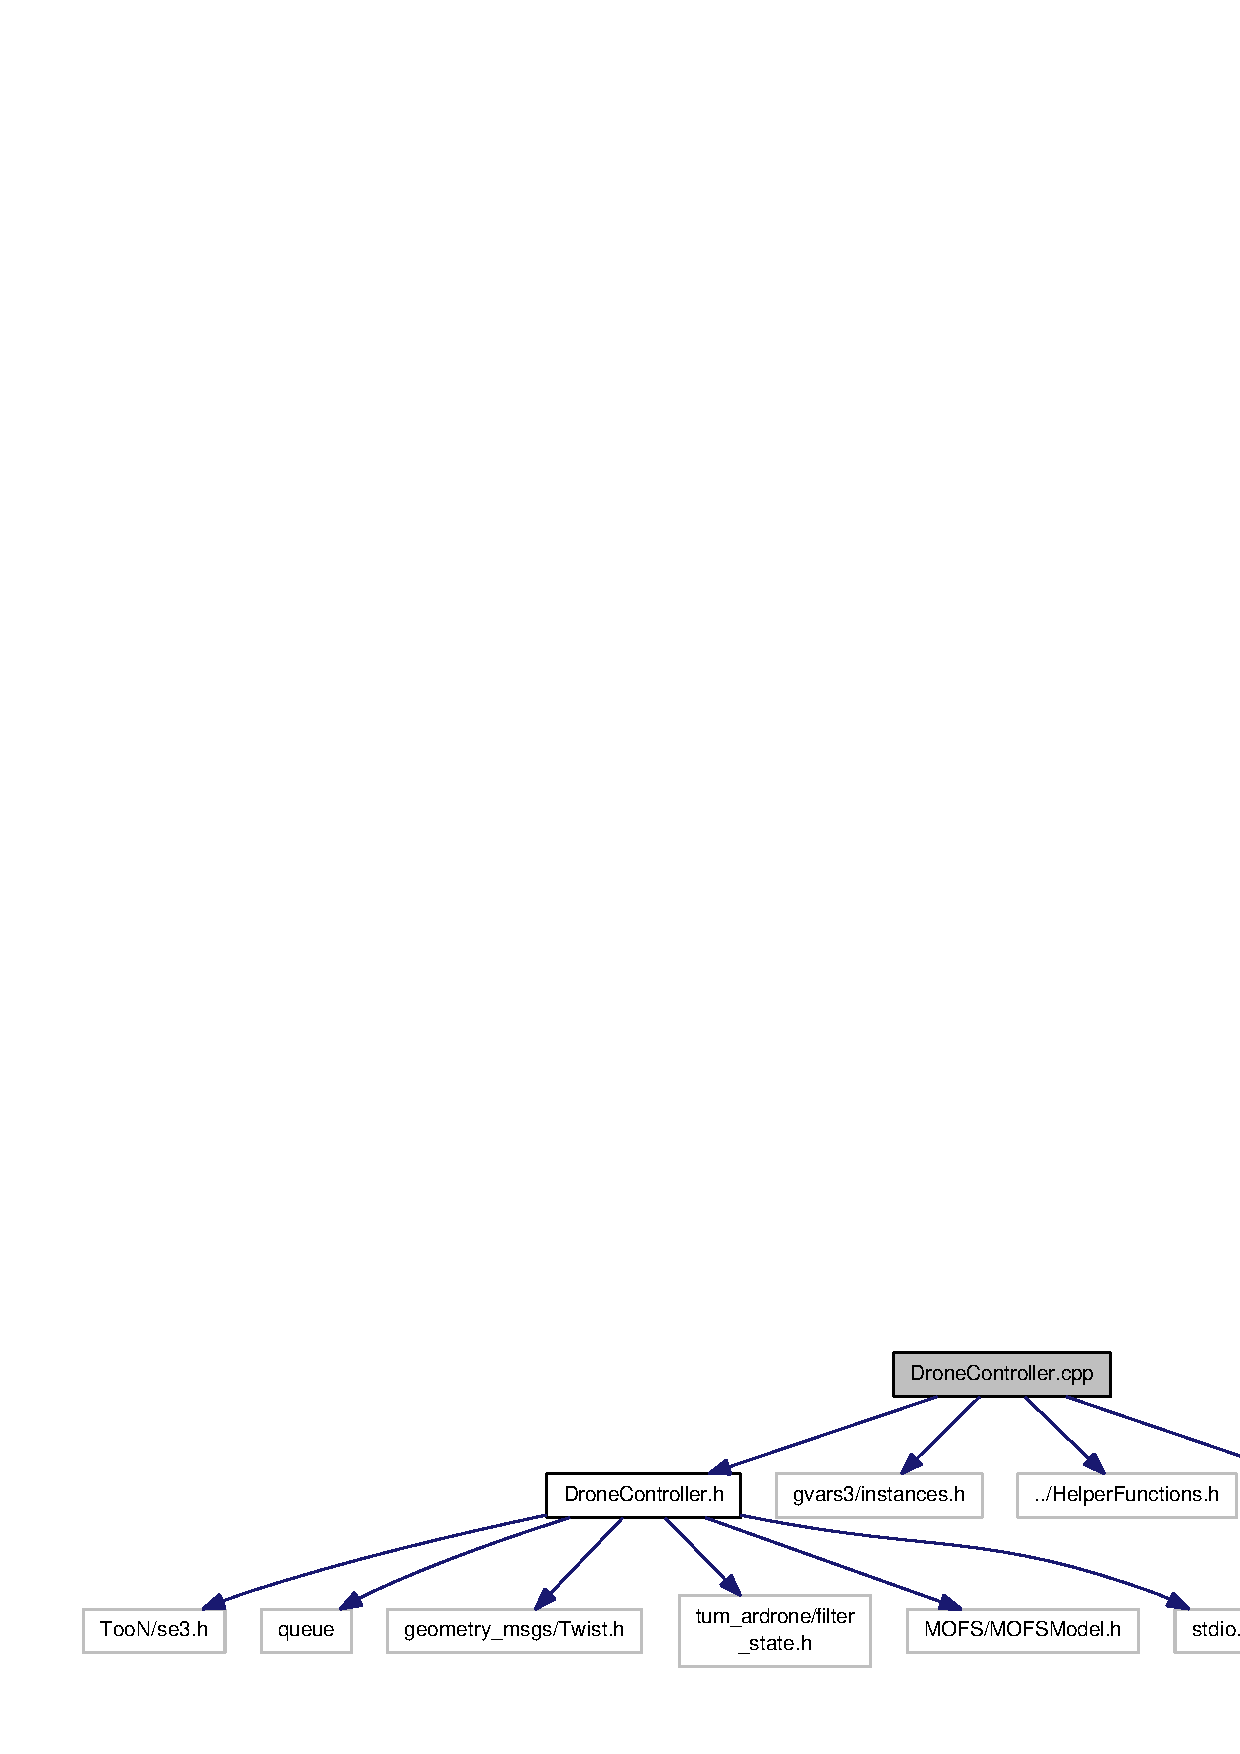
\includegraphics[width=350pt]{DroneController_8cpp__incl}
\end{center}
\end{figure}
\subsection*{Functions}
\begin{DoxyCompactItemize}
\item 
double {\bf angle\-From\-To2} (double angle, double min, double sup)
\item 
void {\bf i\-\_\-term\-\_\-increase} (double \&i\-\_\-term, double new\-\_\-err, double cap)
\end{DoxyCompactItemize}


\subsection{Function Documentation}
\index{Drone\-Controller.\-cpp@{Drone\-Controller.\-cpp}!angle\-From\-To2@{angle\-From\-To2}}
\index{angle\-From\-To2@{angle\-From\-To2}!DroneController.cpp@{Drone\-Controller.\-cpp}}
\subsubsection[{angle\-From\-To2}]{\setlength{\rightskip}{0pt plus 5cm}double angle\-From\-To2 (
\begin{DoxyParamCaption}
\item[{double}]{angle, }
\item[{double}]{min, }
\item[{double}]{sup}
\end{DoxyParamCaption}
)}\label{DroneController_8cpp_a20b6f01f7b9152325efd813634c0ed7f}


Definition at line 62 of file Drone\-Controller.\-cpp.

\index{Drone\-Controller.\-cpp@{Drone\-Controller.\-cpp}!i\-\_\-term\-\_\-increase@{i\-\_\-term\-\_\-increase}}
\index{i\-\_\-term\-\_\-increase@{i\-\_\-term\-\_\-increase}!DroneController.cpp@{Drone\-Controller.\-cpp}}
\subsubsection[{i\-\_\-term\-\_\-increase}]{\setlength{\rightskip}{0pt plus 5cm}void i\-\_\-term\-\_\-increase (
\begin{DoxyParamCaption}
\item[{double \&}]{i\-\_\-term, }
\item[{double}]{new\-\_\-err, }
\item[{double}]{cap}
\end{DoxyParamCaption}
)}\label{DroneController_8cpp_a56f3d1ddd4cc99a10e5248e2c3f84136}


Definition at line 147 of file Drone\-Controller.\-cpp.


\section{Drone\-Controller.\-h File Reference}
\label{DroneController_8h}\index{Drone\-Controller.\-h@{Drone\-Controller.\-h}}
{\ttfamily \#include \char`\"{}Too\-N/se3.\-h\char`\"{}}\\*
{\ttfamily \#include $<$queue$>$}\\*
{\ttfamily \#include \char`\"{}geometry\-\_\-msgs/\-Twist.\-h\char`\"{}}\\*
{\ttfamily \#include \char`\"{}tum\-\_\-ardrone/filter\-\_\-state.\-h\char`\"{}}\\*
{\ttfamily \#include \char`\"{}M\-O\-F\-S/\-M\-O\-F\-S\-Model.\-h\char`\"{}}\\*
{\ttfamily \#include $<$stdio.\-h$>$}\\*
Include dependency graph for Drone\-Controller.\-h\-:\nopagebreak
\begin{figure}[H]
\begin{center}
\leavevmode
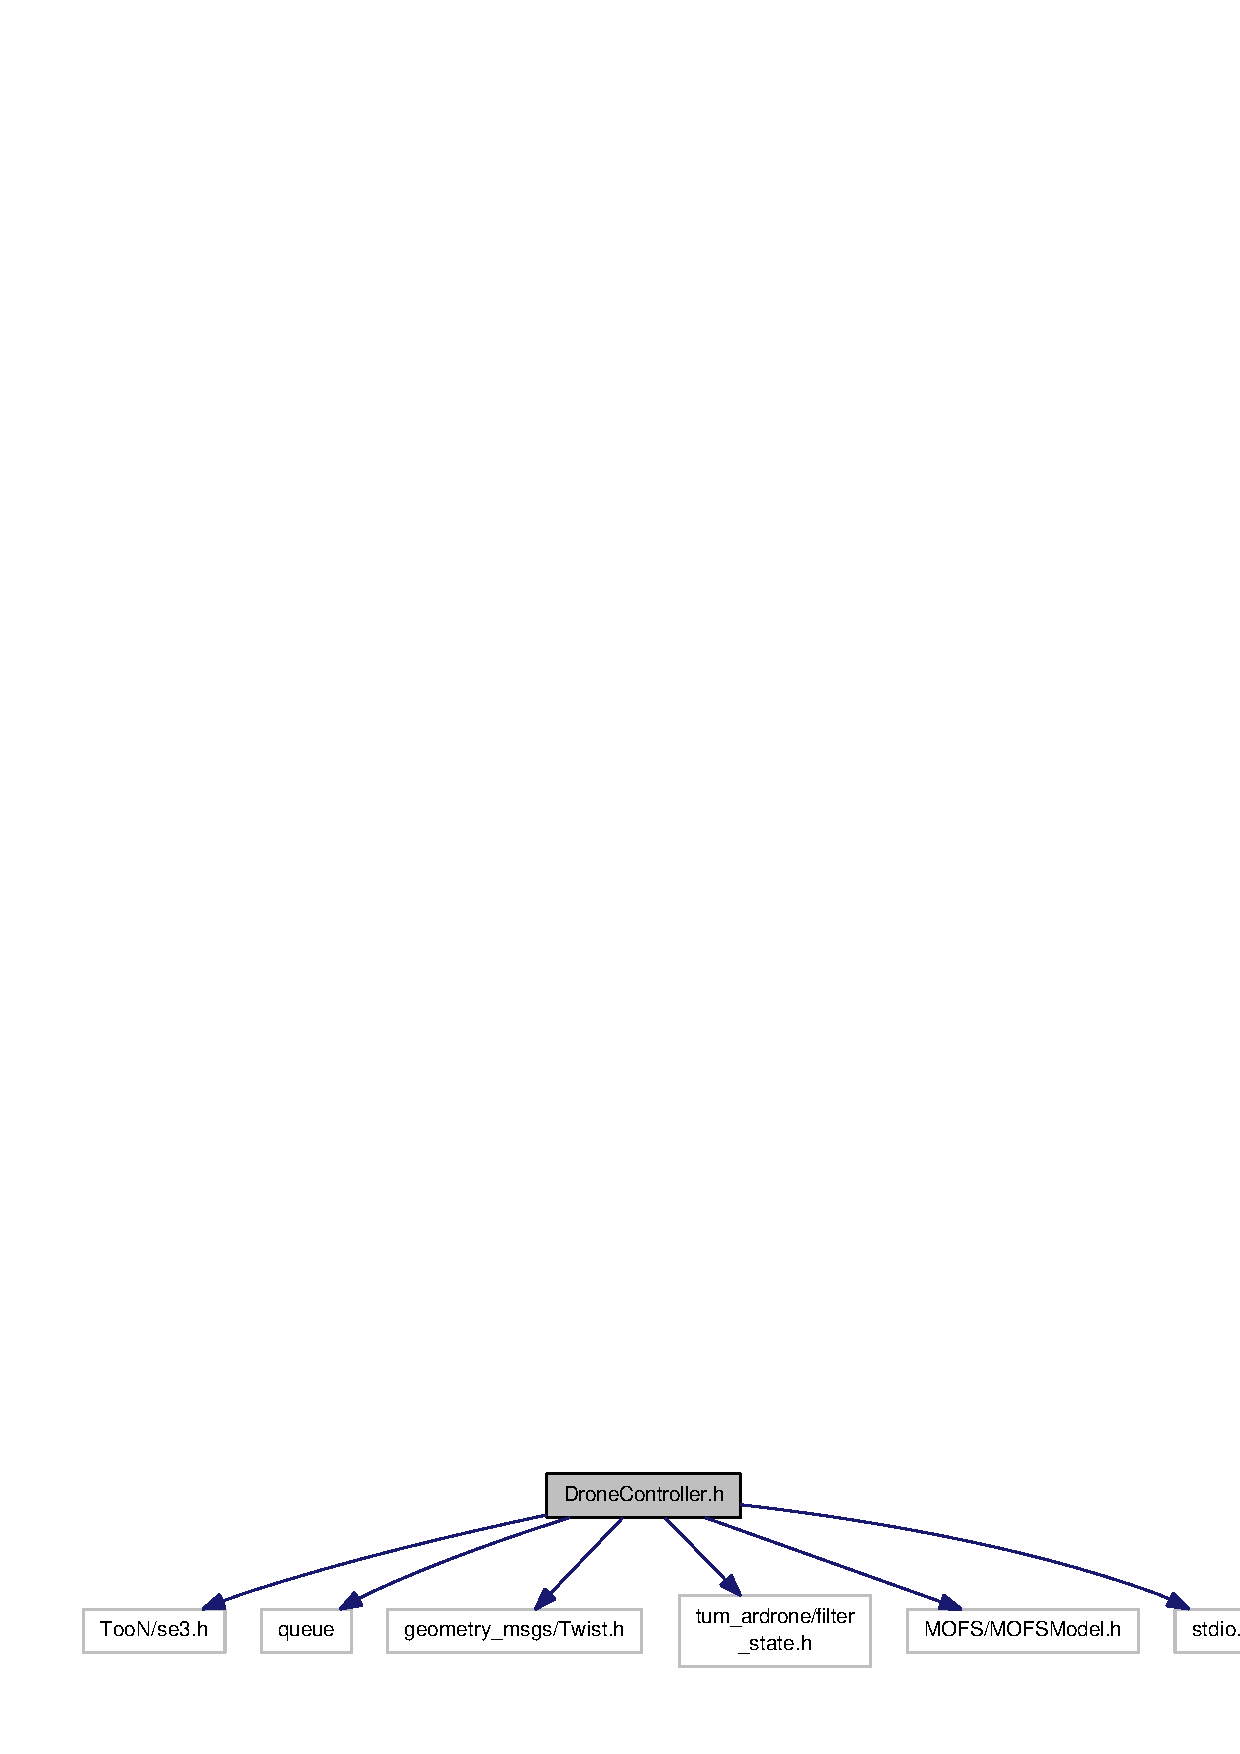
\includegraphics[width=350pt]{DroneController_8h__incl}
\end{center}
\end{figure}
This graph shows which files directly or indirectly include this file\-:\nopagebreak
\begin{figure}[H]
\begin{center}
\leavevmode
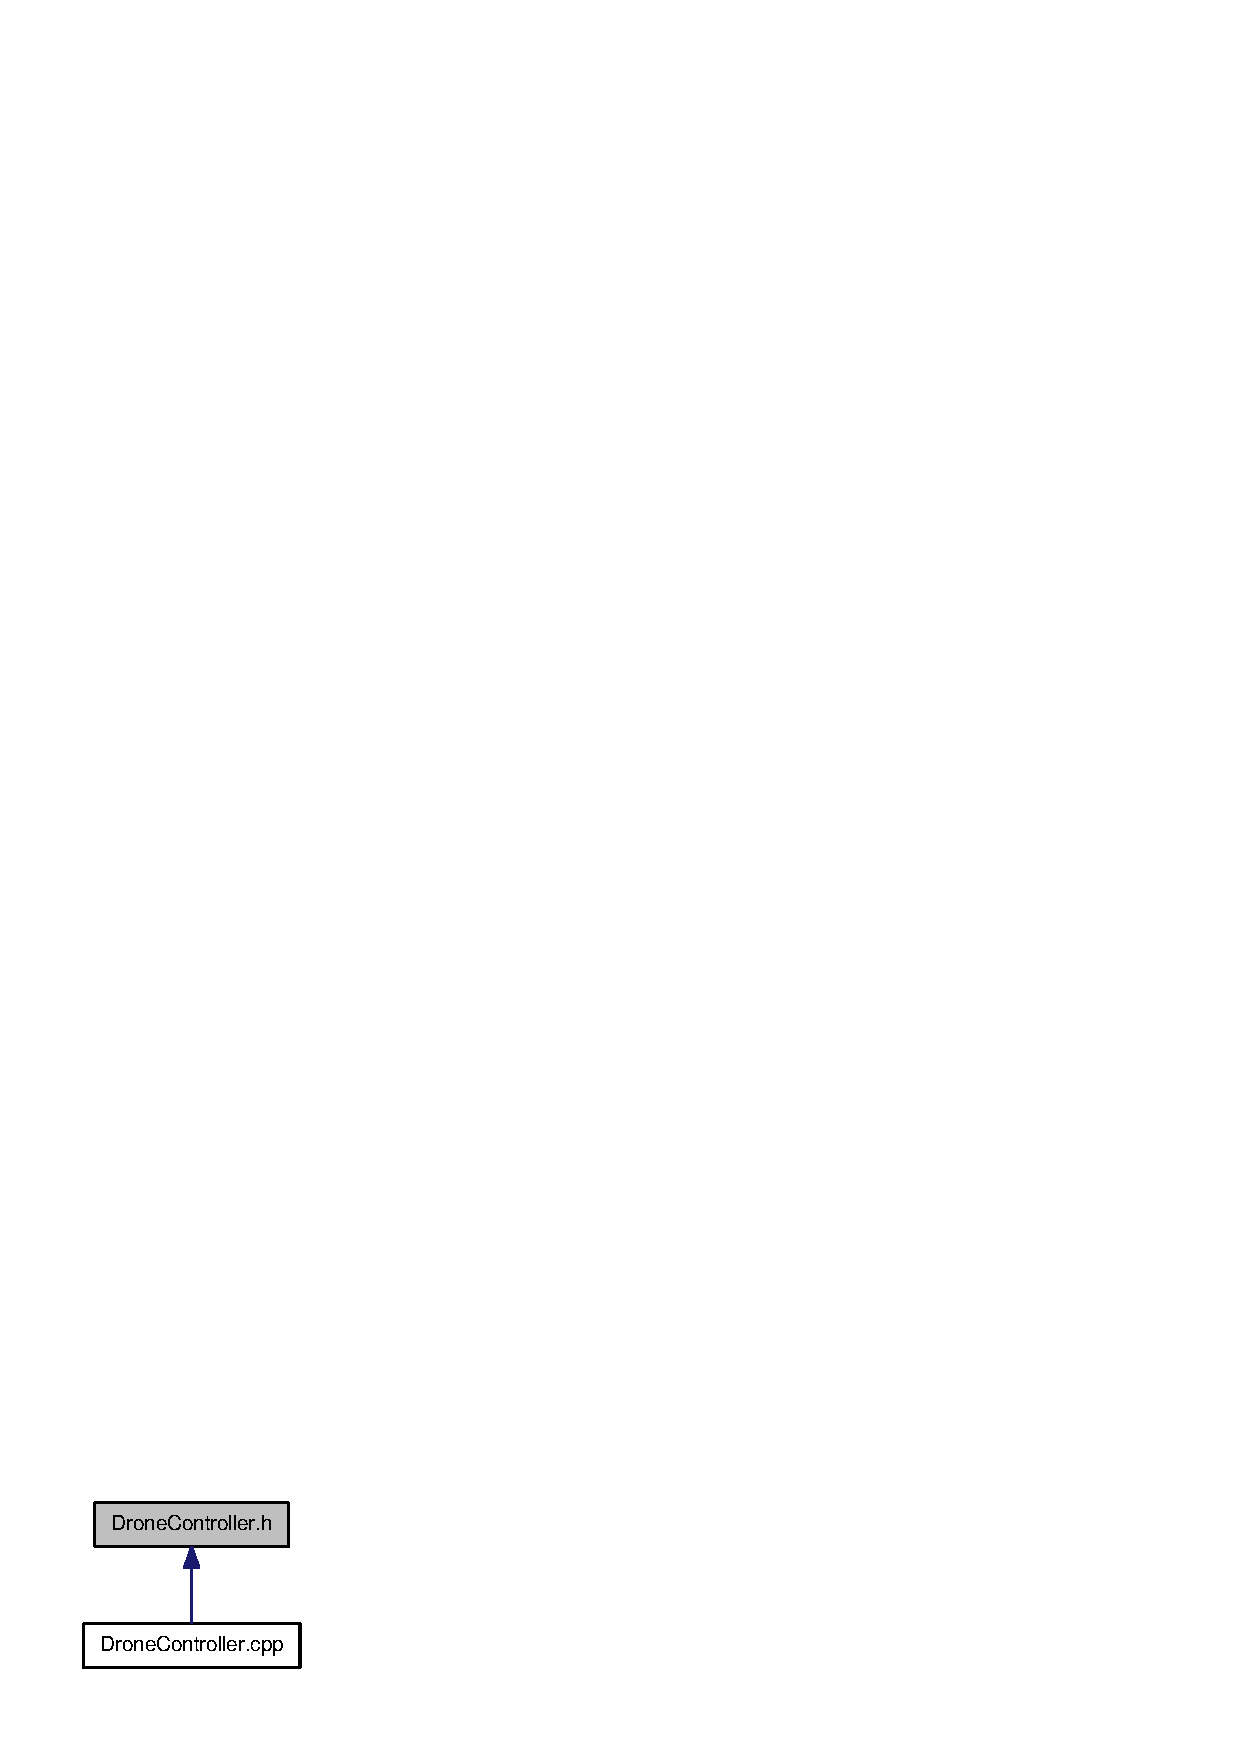
\includegraphics[width=148pt]{DroneController_8h__dep__incl}
\end{center}
\end{figure}
\subsection*{Classes}
\begin{DoxyCompactItemize}
\item 
struct {\bf Control\-Command}
\item 
class {\bf Drone\-Controller}
\item 
struct {\bf Drone\-Position}
\end{DoxyCompactItemize}

\section{Fuzzy\-Control\-\_\-\-I\-O.\-h File Reference}
\label{FuzzyControl__IO_8h}\index{Fuzzy\-Control\-\_\-\-I\-O.\-h@{Fuzzy\-Control\-\_\-\-I\-O.\-h}}
{\ttfamily \#include $<$string$>$}\\*
{\ttfamily \#include $<$vector$>$}\\*
{\ttfamily \#include $<$map$>$}\\*
{\ttfamily \#include $<$ostream$>$}\\*
{\ttfamily \#include \char`\"{}ros/serialization.\-h\char`\"{}}\\*
{\ttfamily \#include \char`\"{}ros/builtin\-\_\-message\-\_\-traits.\-h\char`\"{}}\\*
{\ttfamily \#include \char`\"{}ros/message\-\_\-operations.\-h\char`\"{}}\\*
{\ttfamily \#include \char`\"{}ros/time.\-h\char`\"{}}\\*
{\ttfamily \#include \char`\"{}ros/macros.\-h\char`\"{}}\\*
{\ttfamily \#include \char`\"{}ros/assert.\-h\char`\"{}}\\*
{\ttfamily \#include \char`\"{}ros/service\-\_\-traits.\-h\char`\"{}}\\*
Include dependency graph for Fuzzy\-Control\-\_\-\-I\-O.\-h\-:\nopagebreak
\begin{figure}[H]
\begin{center}
\leavevmode
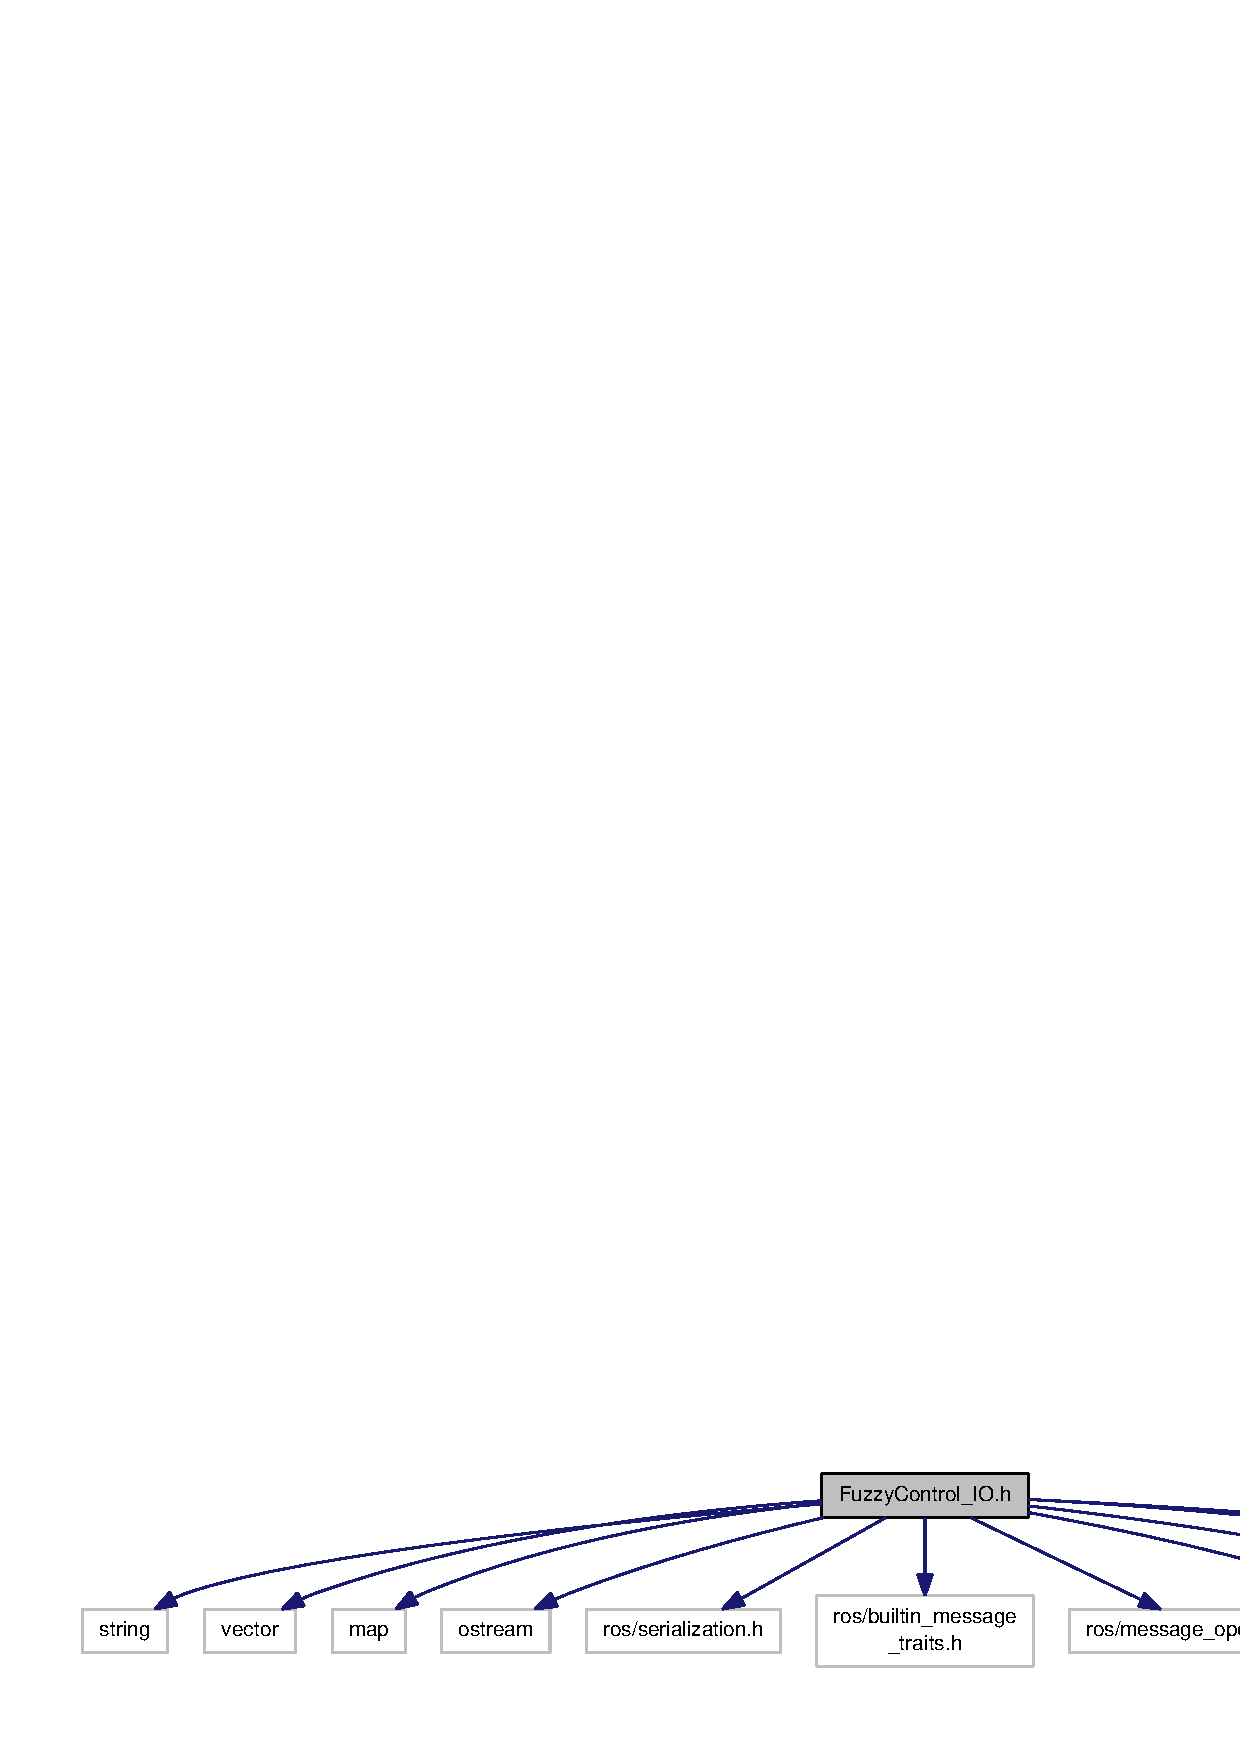
\includegraphics[width=350pt]{FuzzyControl__IO_8h__incl}
\end{center}
\end{figure}
This graph shows which files directly or indirectly include this file\-:\nopagebreak
\begin{figure}[H]
\begin{center}
\leavevmode
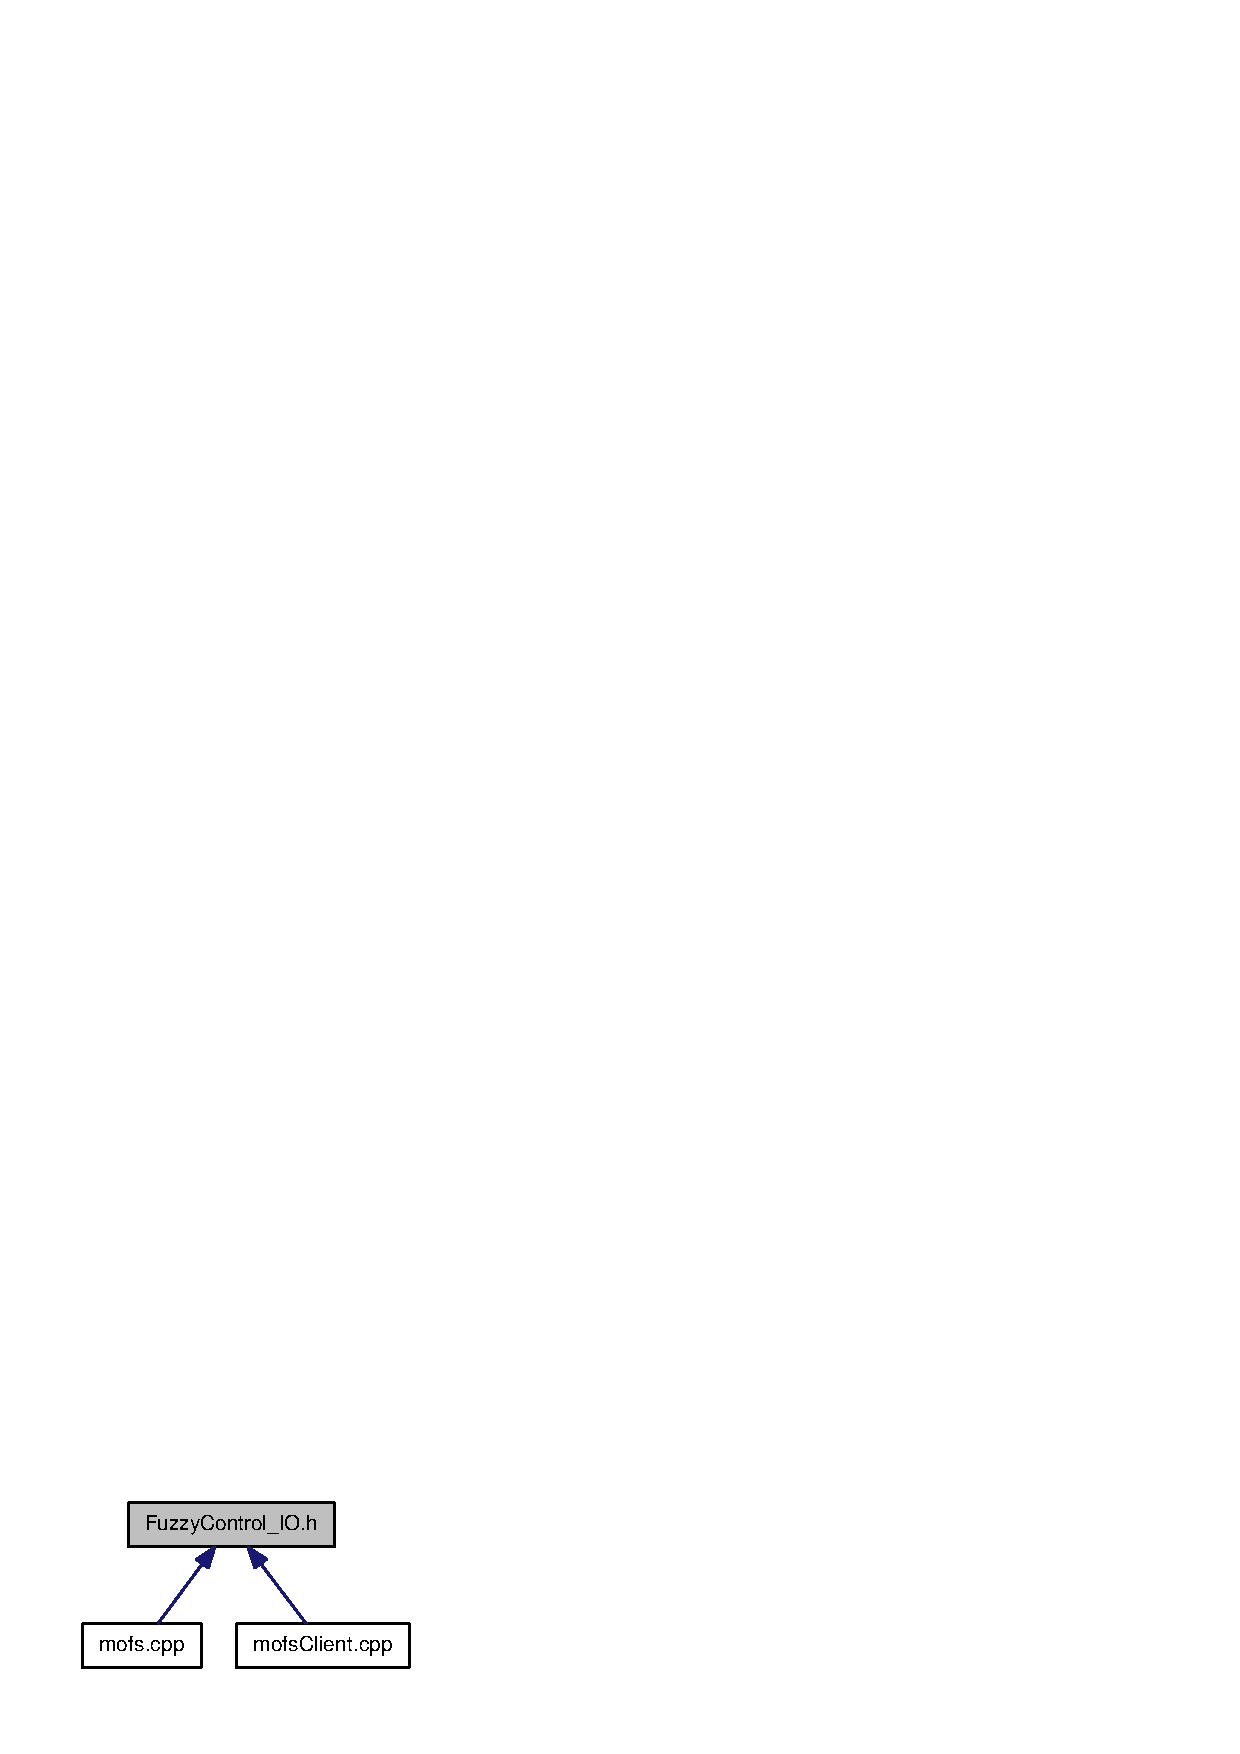
\includegraphics[width=200pt]{FuzzyControl__IO_8h__dep__incl}
\end{center}
\end{figure}
\subsection*{Classes}
\begin{DoxyCompactItemize}
\item 
struct {\bf ros\-::message\-\_\-traits\-::\-Data\-Type$<$ \-::mofs\-::\-Fuzzy\-Control\-\_\-\-I\-O\-Request\-\_\-$<$ Container\-Allocator $>$ $>$}
\item 
struct {\bf ros\-::message\-\_\-traits\-::\-Data\-Type$<$ \-::mofs\-::\-Fuzzy\-Control\-\_\-\-I\-O\-Response\-\_\-$<$ Container\-Allocator $>$ $>$}
\item 
struct {\bf ros\-::service\-\_\-traits\-::\-Data\-Type$<$ mofs\-::\-Fuzzy\-Control\-\_\-\-I\-O $>$}
\item 
struct {\bf ros\-::service\-\_\-traits\-::\-Data\-Type$<$ mofs\-::\-Fuzzy\-Control\-\_\-\-I\-O\-Request\-\_\-$<$ Container\-Allocator $>$ $>$}
\item 
struct {\bf ros\-::service\-\_\-traits\-::\-Data\-Type$<$ mofs\-::\-Fuzzy\-Control\-\_\-\-I\-O\-Response\-\_\-$<$ Container\-Allocator $>$ $>$}
\item 
struct {\bf ros\-::message\-\_\-traits\-::\-Definition$<$ \-::mofs\-::\-Fuzzy\-Control\-\_\-\-I\-O\-Request\-\_\-$<$ Container\-Allocator $>$ $>$}
\item 
struct {\bf ros\-::message\-\_\-traits\-::\-Definition$<$ \-::mofs\-::\-Fuzzy\-Control\-\_\-\-I\-O\-Response\-\_\-$<$ Container\-Allocator $>$ $>$}
\item 
struct {\bf mofs\-::\-Fuzzy\-Control\-\_\-\-I\-O}
\item 
struct {\bf mofs\-::\-Fuzzy\-Control\-\_\-\-I\-O\-Request\-\_\-$<$ Container\-Allocator $>$}
\item 
struct {\bf mofs\-::\-Fuzzy\-Control\-\_\-\-I\-O\-Response\-\_\-$<$ Container\-Allocator $>$}
\item 
struct {\bf ros\-::message\-\_\-traits\-::\-Is\-Fixed\-Size$<$ \-::mofs\-::\-Fuzzy\-Control\-\_\-\-I\-O\-Request\-\_\-$<$ Container\-Allocator $>$ $>$}
\item 
struct {\bf ros\-::message\-\_\-traits\-::\-Is\-Fixed\-Size$<$ \-::mofs\-::\-Fuzzy\-Control\-\_\-\-I\-O\-Response\-\_\-$<$ Container\-Allocator $>$ $>$}
\item 
struct {\bf ros\-::message\-\_\-traits\-::\-Is\-Message$<$ \-::mofs\-::\-Fuzzy\-Control\-\_\-\-I\-O\-Request\-\_\-$<$ Container\-Allocator $>$ $>$}
\item 
struct {\bf ros\-::message\-\_\-traits\-::\-Is\-Message$<$ \-::mofs\-::\-Fuzzy\-Control\-\_\-\-I\-O\-Request\-\_\-$<$ Container\-Allocator $>$const  $>$}
\item 
struct {\bf ros\-::message\-\_\-traits\-::\-Is\-Message$<$ \-::mofs\-::\-Fuzzy\-Control\-\_\-\-I\-O\-Response\-\_\-$<$ Container\-Allocator $>$ $>$}
\item 
struct {\bf ros\-::message\-\_\-traits\-::\-Is\-Message$<$ \-::mofs\-::\-Fuzzy\-Control\-\_\-\-I\-O\-Response\-\_\-$<$ Container\-Allocator $>$const  $>$}
\item 
struct {\bf ros\-::message\-\_\-traits\-::\-M\-D5\-Sum$<$ \-::mofs\-::\-Fuzzy\-Control\-\_\-\-I\-O\-Request\-\_\-$<$ Container\-Allocator $>$ $>$}
\item 
struct {\bf ros\-::message\-\_\-traits\-::\-M\-D5\-Sum$<$ \-::mofs\-::\-Fuzzy\-Control\-\_\-\-I\-O\-Response\-\_\-$<$ Container\-Allocator $>$ $>$}
\item 
struct {\bf ros\-::service\-\_\-traits\-::\-M\-D5\-Sum$<$ mofs\-::\-Fuzzy\-Control\-\_\-\-I\-O $>$}
\item 
struct {\bf ros\-::service\-\_\-traits\-::\-M\-D5\-Sum$<$ mofs\-::\-Fuzzy\-Control\-\_\-\-I\-O\-Request\-\_\-$<$ Container\-Allocator $>$ $>$}
\item 
struct {\bf ros\-::service\-\_\-traits\-::\-M\-D5\-Sum$<$ mofs\-::\-Fuzzy\-Control\-\_\-\-I\-O\-Response\-\_\-$<$ Container\-Allocator $>$ $>$}
\item 
struct {\bf ros\-::serialization\-::\-Serializer$<$ \-::mofs\-::\-Fuzzy\-Control\-\_\-\-I\-O\-Request\-\_\-$<$ Container\-Allocator $>$ $>$}
\item 
struct {\bf ros\-::serialization\-::\-Serializer$<$ \-::mofs\-::\-Fuzzy\-Control\-\_\-\-I\-O\-Response\-\_\-$<$ Container\-Allocator $>$ $>$}
\end{DoxyCompactItemize}
\subsection*{Namespaces}
\begin{DoxyCompactItemize}
\item 
{\bf mofs}
\item 
{\bf ros}
\item 
{\bf ros\-::message\-\_\-traits}
\item 
{\bf ros\-::serialization}
\item 
{\bf ros\-::service\-\_\-traits}
\end{DoxyCompactItemize}
\subsection*{Typedefs}
\begin{DoxyCompactItemize}
\item 
typedef \\*
\-::{\bf mofs\-::\-Fuzzy\-Control\-\_\-\-I\-O\-Request\-\_\-}\\*
$<$ std\-::allocator$<$ void $>$ $>$ {\bf mofs\-::\-Fuzzy\-Control\-\_\-\-I\-O\-Request}
\item 
typedef boost\-::shared\-\_\-ptr\\*
$<$ \-::{\bf mofs\-::\-Fuzzy\-Control\-\_\-\-I\-O\-Request} \\*
const  $>$ {\bf mofs\-::\-Fuzzy\-Control\-\_\-\-I\-O\-Request\-Const\-Ptr}
\item 
typedef boost\-::shared\-\_\-ptr\\*
$<$ \-::{\bf mofs\-::\-Fuzzy\-Control\-\_\-\-I\-O\-Request} $>$ {\bf mofs\-::\-Fuzzy\-Control\-\_\-\-I\-O\-Request\-Ptr}
\item 
typedef \\*
\-::{\bf mofs\-::\-Fuzzy\-Control\-\_\-\-I\-O\-Response\-\_\-}\\*
$<$ std\-::allocator$<$ void $>$ $>$ {\bf mofs\-::\-Fuzzy\-Control\-\_\-\-I\-O\-Response}
\item 
typedef boost\-::shared\-\_\-ptr\\*
$<$ \-::{\bf mofs\-::\-Fuzzy\-Control\-\_\-\-I\-O\-Response} \\*
const  $>$ {\bf mofs\-::\-Fuzzy\-Control\-\_\-\-I\-O\-Response\-Const\-Ptr}
\item 
typedef boost\-::shared\-\_\-ptr\\*
$<$ \-::{\bf mofs\-::\-Fuzzy\-Control\-\_\-\-I\-O\-Response} $>$ {\bf mofs\-::\-Fuzzy\-Control\-\_\-\-I\-O\-Response\-Ptr}
\end{DoxyCompactItemize}

\section{mainpage.\-dox File Reference}
\label{mainpage_8dox}\index{mainpage.\-dox@{mainpage.\-dox}}

\section{mofs.\-cpp File Reference}
\label{mofs_8cpp}\index{mofs.\-cpp@{mofs.\-cpp}}
{\ttfamily \#include \char`\"{}ros/ros.\-h\char`\"{}}\\*
{\ttfamily \#include $<$M\-O\-F\-S\-Model.\-h$>$}\\*
{\ttfamily \#include $<$string.\-h$>$}\\*
{\ttfamily \#include \char`\"{}mofs/\-Fuzzy\-Control\-\_\-\-I\-O.\-h\char`\"{}}\\*
Include dependency graph for mofs.\-cpp\-:\nopagebreak
\begin{figure}[H]
\begin{center}
\leavevmode
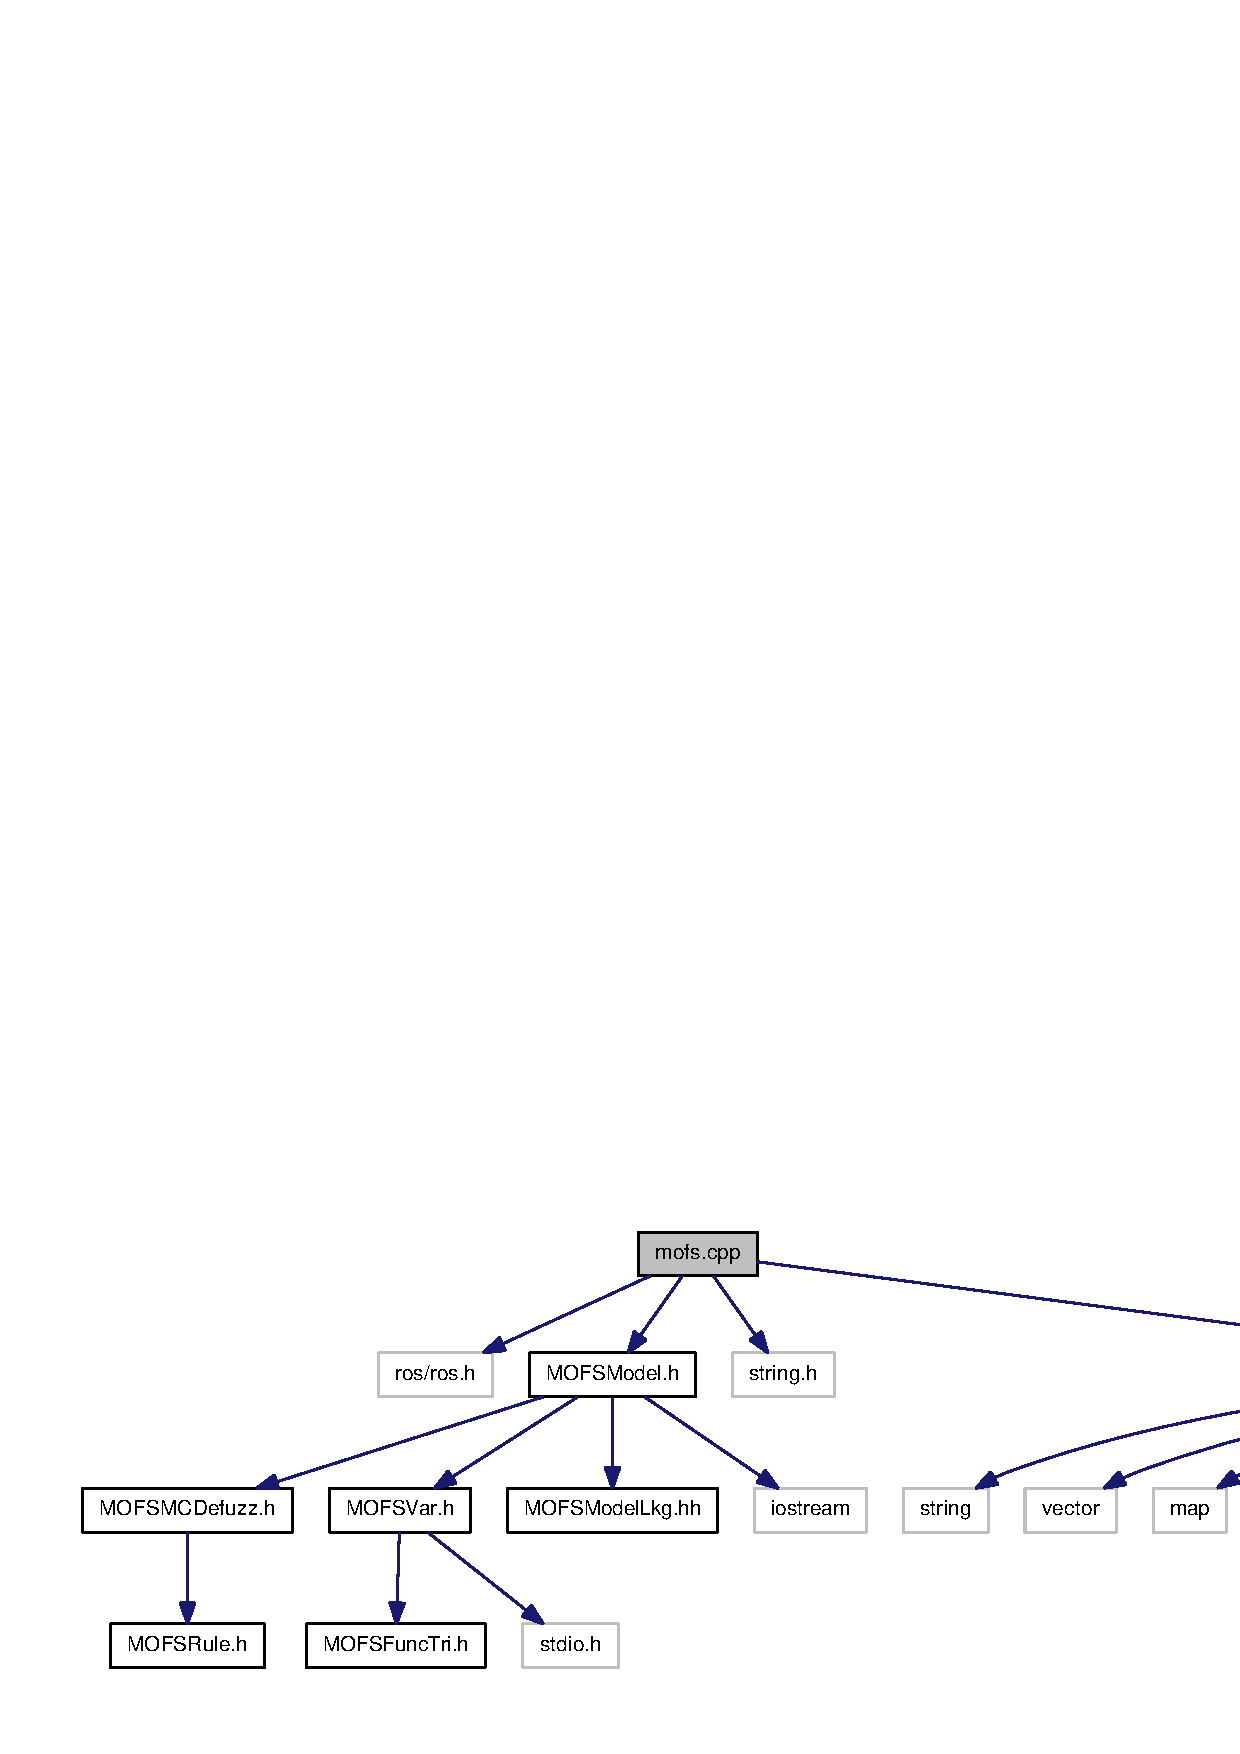
\includegraphics[width=350pt]{mofs_8cpp__incl}
\end{center}
\end{figure}
\subsection*{Functions}
\begin{DoxyCompactItemize}
\item 
bool {\bf fuzzy\-\_\-control\-\_\-\-I\-O\-\_\-callback} ({\bf mofs\-::\-Fuzzy\-Control\-\_\-\-I\-O\-::\-Request} \&request, {\bf mofs\-::\-Fuzzy\-Control\-\_\-\-I\-O\-::\-Response} \&response)
\item 
int {\bf main} (int argc, char $\ast$$\ast$argv)
\end{DoxyCompactItemize}
\subsection*{Variables}
\begin{DoxyCompactItemize}
\item 
char {\bf controller} [100]
\item 
char $\ast$ {\bf file\-Controller}
\item 
char $\ast$ {\bf file\-Rules}
\item 
{\bf mofs\-::\-M\-O\-F\-S\-Model} {\bf flc}
\begin{DoxyCompactList}\small\item\em main file of the mofs-\/\-R\-O\-S package \end{DoxyCompactList}\item 
const char $\ast$ {\bf location} = \char`\"{}/home/miguelolivaresmendez/code/fuerte\-\_\-workspace/sandbox/mofs/include/F\-L\-C/\char`\"{}
\item 
char {\bf rules} [100]
\item 
char $\ast$ {\bf service\-Name}
\end{DoxyCompactItemize}


\subsection{Function Documentation}
\index{mofs.\-cpp@{mofs.\-cpp}!fuzzy\-\_\-control\-\_\-\-I\-O\-\_\-callback@{fuzzy\-\_\-control\-\_\-\-I\-O\-\_\-callback}}
\index{fuzzy\-\_\-control\-\_\-\-I\-O\-\_\-callback@{fuzzy\-\_\-control\-\_\-\-I\-O\-\_\-callback}!mofs.cpp@{mofs.\-cpp}}
\subsubsection[{fuzzy\-\_\-control\-\_\-\-I\-O\-\_\-callback}]{\setlength{\rightskip}{0pt plus 5cm}bool fuzzy\-\_\-control\-\_\-\-I\-O\-\_\-callback (
\begin{DoxyParamCaption}
\item[{{\bf mofs\-::\-Fuzzy\-Control\-\_\-\-I\-O\-::\-Request} \&}]{request, }
\item[{{\bf mofs\-::\-Fuzzy\-Control\-\_\-\-I\-O\-::\-Response} \&}]{response}
\end{DoxyParamCaption}
)}\label{mofs_8cpp_a316fc002b1cd72aa7f757fdab1567217}


Definition at line 34 of file mofs.\-cpp.

\index{mofs.\-cpp@{mofs.\-cpp}!main@{main}}
\index{main@{main}!mofs.cpp@{mofs.\-cpp}}
\subsubsection[{main}]{\setlength{\rightskip}{0pt plus 5cm}int main (
\begin{DoxyParamCaption}
\item[{int}]{argc, }
\item[{char $\ast$$\ast$}]{argv}
\end{DoxyParamCaption}
)}\label{mofs_8cpp_a3c04138a5bfe5d72780bb7e82a18e627}


Definition at line 52 of file mofs.\-cpp.



\subsection{Variable Documentation}
\index{mofs.\-cpp@{mofs.\-cpp}!controller@{controller}}
\index{controller@{controller}!mofs.cpp@{mofs.\-cpp}}
\subsubsection[{controller}]{\setlength{\rightskip}{0pt plus 5cm}char controller[100]}\label{mofs_8cpp_a3b2173f23316172095d407fa5fcab2e9}


Definition at line 32 of file mofs.\-cpp.

\index{mofs.\-cpp@{mofs.\-cpp}!file\-Controller@{file\-Controller}}
\index{file\-Controller@{file\-Controller}!mofs.cpp@{mofs.\-cpp}}
\subsubsection[{file\-Controller}]{\setlength{\rightskip}{0pt plus 5cm}char$\ast$ file\-Controller}\label{mofs_8cpp_a93896147a3e179d74e6438148ea1c610}


Definition at line 29 of file mofs.\-cpp.

\index{mofs.\-cpp@{mofs.\-cpp}!file\-Rules@{file\-Rules}}
\index{file\-Rules@{file\-Rules}!mofs.cpp@{mofs.\-cpp}}
\subsubsection[{file\-Rules}]{\setlength{\rightskip}{0pt plus 5cm}char $\ast$ file\-Rules}\label{mofs_8cpp_a8eb26277378a227518c3aa6f090c2661}


Definition at line 29 of file mofs.\-cpp.

\index{mofs.\-cpp@{mofs.\-cpp}!flc@{flc}}
\index{flc@{flc}!mofs.cpp@{mofs.\-cpp}}
\subsubsection[{flc}]{\setlength{\rightskip}{0pt plus 5cm}{\bf mofs\-::\-M\-O\-F\-S\-Model} flc}\label{mofs_8cpp_a6f52a2f969cd19dfff86253295b31367}


main file of the mofs-\/\-R\-O\-S package 

\doxyref{mofs.\-cpp}{p.}{mofs_8cpp}

Created on\-: 27 May 2013 Author\-: Miguel A. Olivares-\/\-Mendez Sn\-T -\/ University of Luxembourg Automation Research Group

mofs was previously a C++ library and now a R\-O\-S package developed by Miguel Angel Olivares-\/\-Mendez at the Computer Vision Group -\/ Universidad Politecnica de Madrid and at Automation Research Group
\begin{DoxyItemize}
\item Sn\-T -\/ University of Luxembourg. This software allow to create and use Fuzzy Logic controllers to command whatever you want
\end{DoxyItemize}

Used under the conditions of R\-O\-S

any doubts don't hesitate to contact me\-: {\tt miguel.\-olivaresmendez@uni.\-lu} 

Definition at line 28 of file mofs.\-cpp.

\index{mofs.\-cpp@{mofs.\-cpp}!location@{location}}
\index{location@{location}!mofs.cpp@{mofs.\-cpp}}
\subsubsection[{location}]{\setlength{\rightskip}{0pt plus 5cm}const char$\ast$ location = \char`\"{}/home/miguelolivaresmendez/code/fuerte\-\_\-workspace/sandbox/mofs/include/F\-L\-C/\char`\"{}}\label{mofs_8cpp_ae01f83c0db62232963d563c132709d38}


Definition at line 31 of file mofs.\-cpp.

\index{mofs.\-cpp@{mofs.\-cpp}!rules@{rules}}
\index{rules@{rules}!mofs.cpp@{mofs.\-cpp}}
\subsubsection[{rules}]{\setlength{\rightskip}{0pt plus 5cm}char rules[100]}\label{mofs_8cpp_af43d7dc82f5877eaac4e7cb250f79b05}


Definition at line 32 of file mofs.\-cpp.

\index{mofs.\-cpp@{mofs.\-cpp}!service\-Name@{service\-Name}}
\index{service\-Name@{service\-Name}!mofs.cpp@{mofs.\-cpp}}
\subsubsection[{service\-Name}]{\setlength{\rightskip}{0pt plus 5cm}char $\ast$ service\-Name}\label{mofs_8cpp_a08e50bfb5333289d9c10f9314fd13fbf}


Definition at line 29 of file mofs.\-cpp.


\section{mofs\-Client.\-cpp File Reference}
\label{mofsClient_8cpp}\index{mofs\-Client.\-cpp@{mofs\-Client.\-cpp}}
{\ttfamily \#include \char`\"{}ros/ros.\-h\char`\"{}}\\*
{\ttfamily \#include \char`\"{}mofs/\-Fuzzy\-Control\-\_\-\-I\-O.\-h\char`\"{}}\\*
{\ttfamily \#include $<$cstdlib$>$}\\*
Include dependency graph for mofs\-Client.\-cpp\-:\nopagebreak
\begin{figure}[H]
\begin{center}
\leavevmode
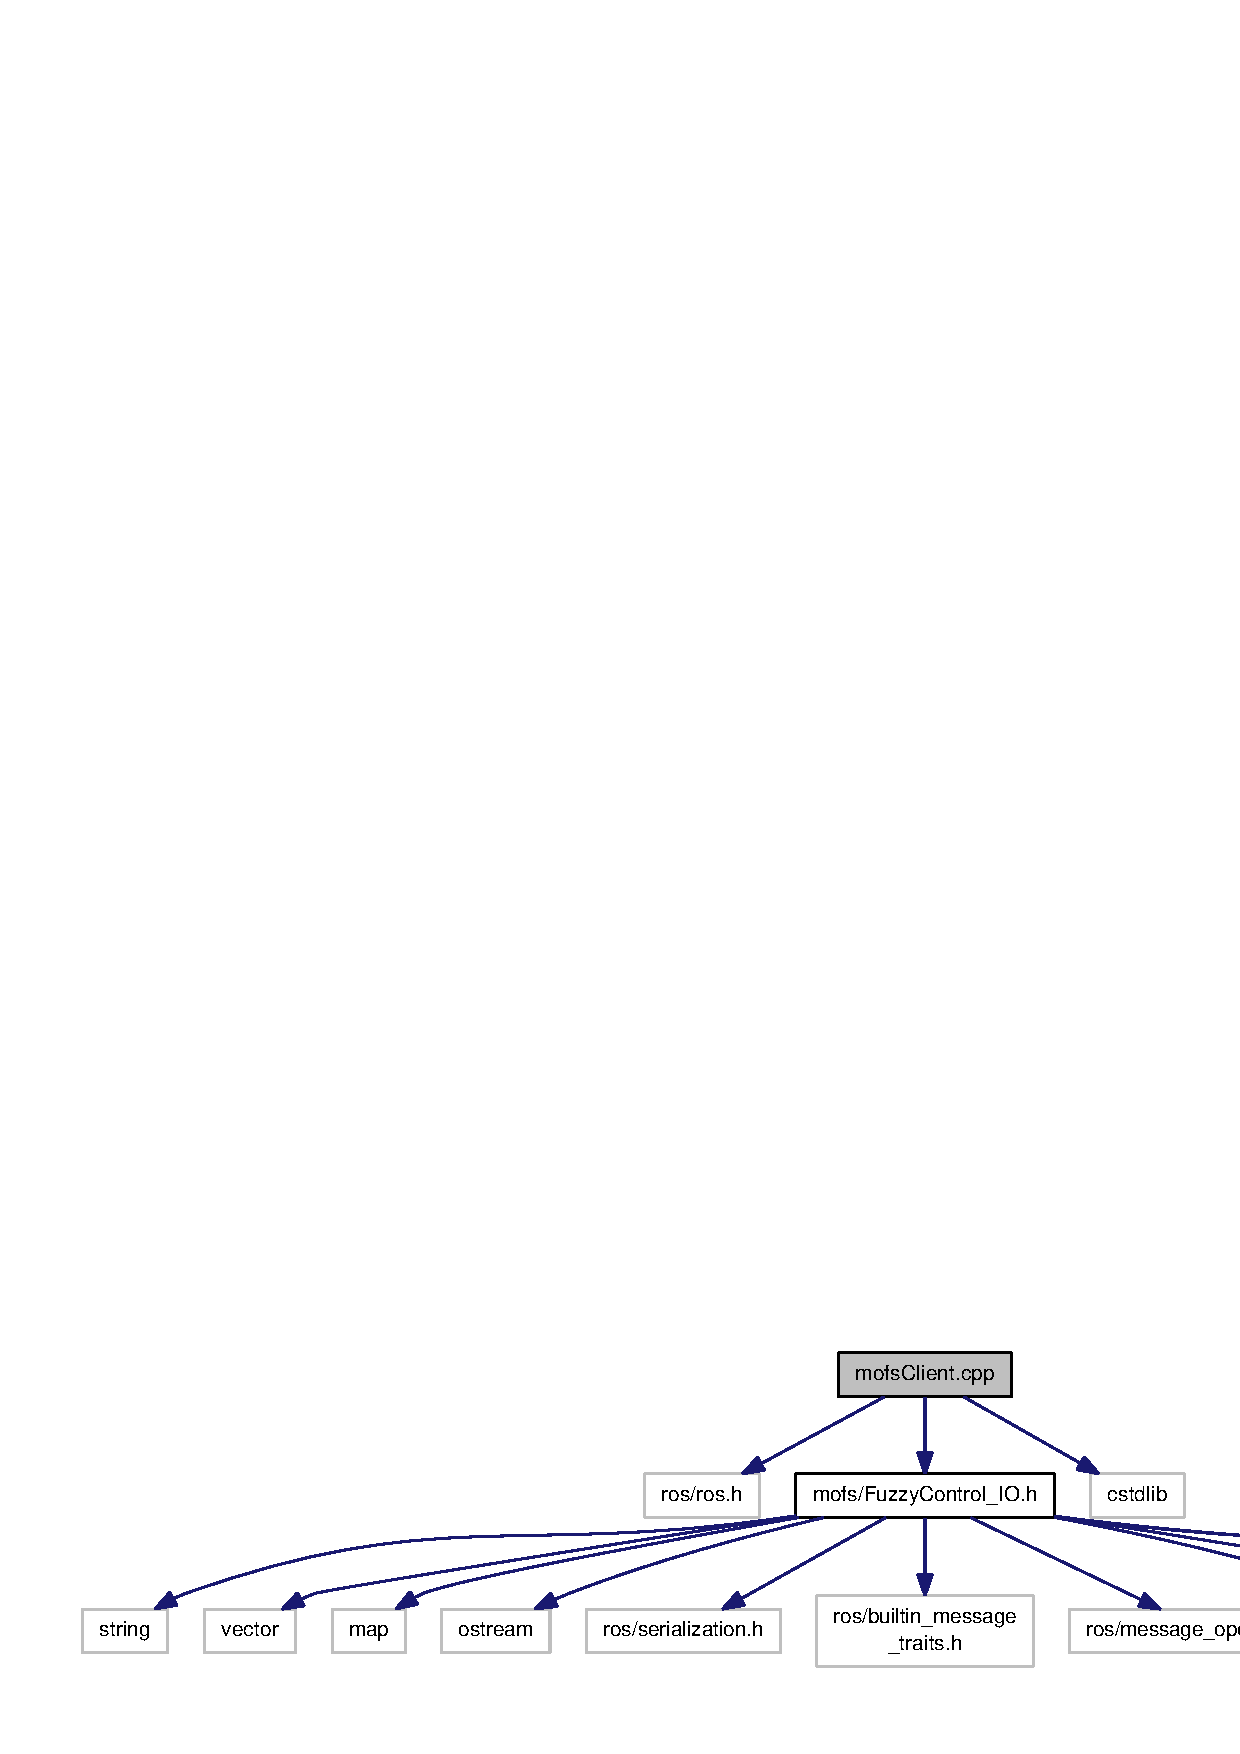
\includegraphics[width=350pt]{mofsClient_8cpp__incl}
\end{center}
\end{figure}
\subsection*{Functions}
\begin{DoxyCompactItemize}
\item 
int {\bf main} (int argc, char $\ast$$\ast$argv)
\begin{DoxyCompactList}\small\item\em example of a client to communicate with the mofs-\/\-R\-O\-S package \end{DoxyCompactList}\end{DoxyCompactItemize}


\subsection{Function Documentation}
\index{mofs\-Client.\-cpp@{mofs\-Client.\-cpp}!main@{main}}
\index{main@{main}!mofsClient.cpp@{mofs\-Client.\-cpp}}
\subsubsection[{main}]{\setlength{\rightskip}{0pt plus 5cm}int main (
\begin{DoxyParamCaption}
\item[{int}]{argc, }
\item[{char $\ast$$\ast$}]{argv}
\end{DoxyParamCaption}
)}\label{mofsClient_8cpp_a3c04138a5bfe5d72780bb7e82a18e627}


example of a client to communicate with the mofs-\/\-R\-O\-S package 

\doxyref{mofs.\-cpp}{p.}{mofs_8cpp}

Created on\-: 27 May 2013 Author\-: Miguel A. Olivares-\/\-Mendez Sn\-T -\/ University of Luxembourg Automation Research Group

mofs was previously a C++ library and now a R\-O\-S package developed by Miguel Angel Olivares Mendez at the Computer Vision Group -\/ Universidad Politecnica de Madrid and at Automation Research Group
\begin{DoxyItemize}
\item Sn\-T -\/ University of Luxembourg. This software allow to create and use Fuzzy Logic controllers to command whatever you want
\end{DoxyItemize}

Used under the conditions of R\-O\-S

any doubts don't hesitate to contact me\-: {\tt miguel.\-olivaresmendez@uni.\-lu} 

Definition at line 27 of file mofs\-Client.\-cpp.


\section{M\-O\-F\-S\-Func\-Tri.\-cpp File Reference}
\label{MOFSFuncTri_8cpp}\index{M\-O\-F\-S\-Func\-Tri.\-cpp@{M\-O\-F\-S\-Func\-Tri.\-cpp}}
{\ttfamily \#include \char`\"{}M\-O\-F\-S\-Func\-Tri.\-h\char`\"{}}\\*
{\ttfamily \#include \char`\"{}M\-O\-F\-S\-Rule.\-h\char`\"{}}\\*
{\ttfamily \#include $<$cstdlib$>$}\\*
{\ttfamily \#include $<$iostream$>$}\\*
Include dependency graph for M\-O\-F\-S\-Func\-Tri.\-cpp\-:\nopagebreak
\begin{figure}[H]
\begin{center}
\leavevmode
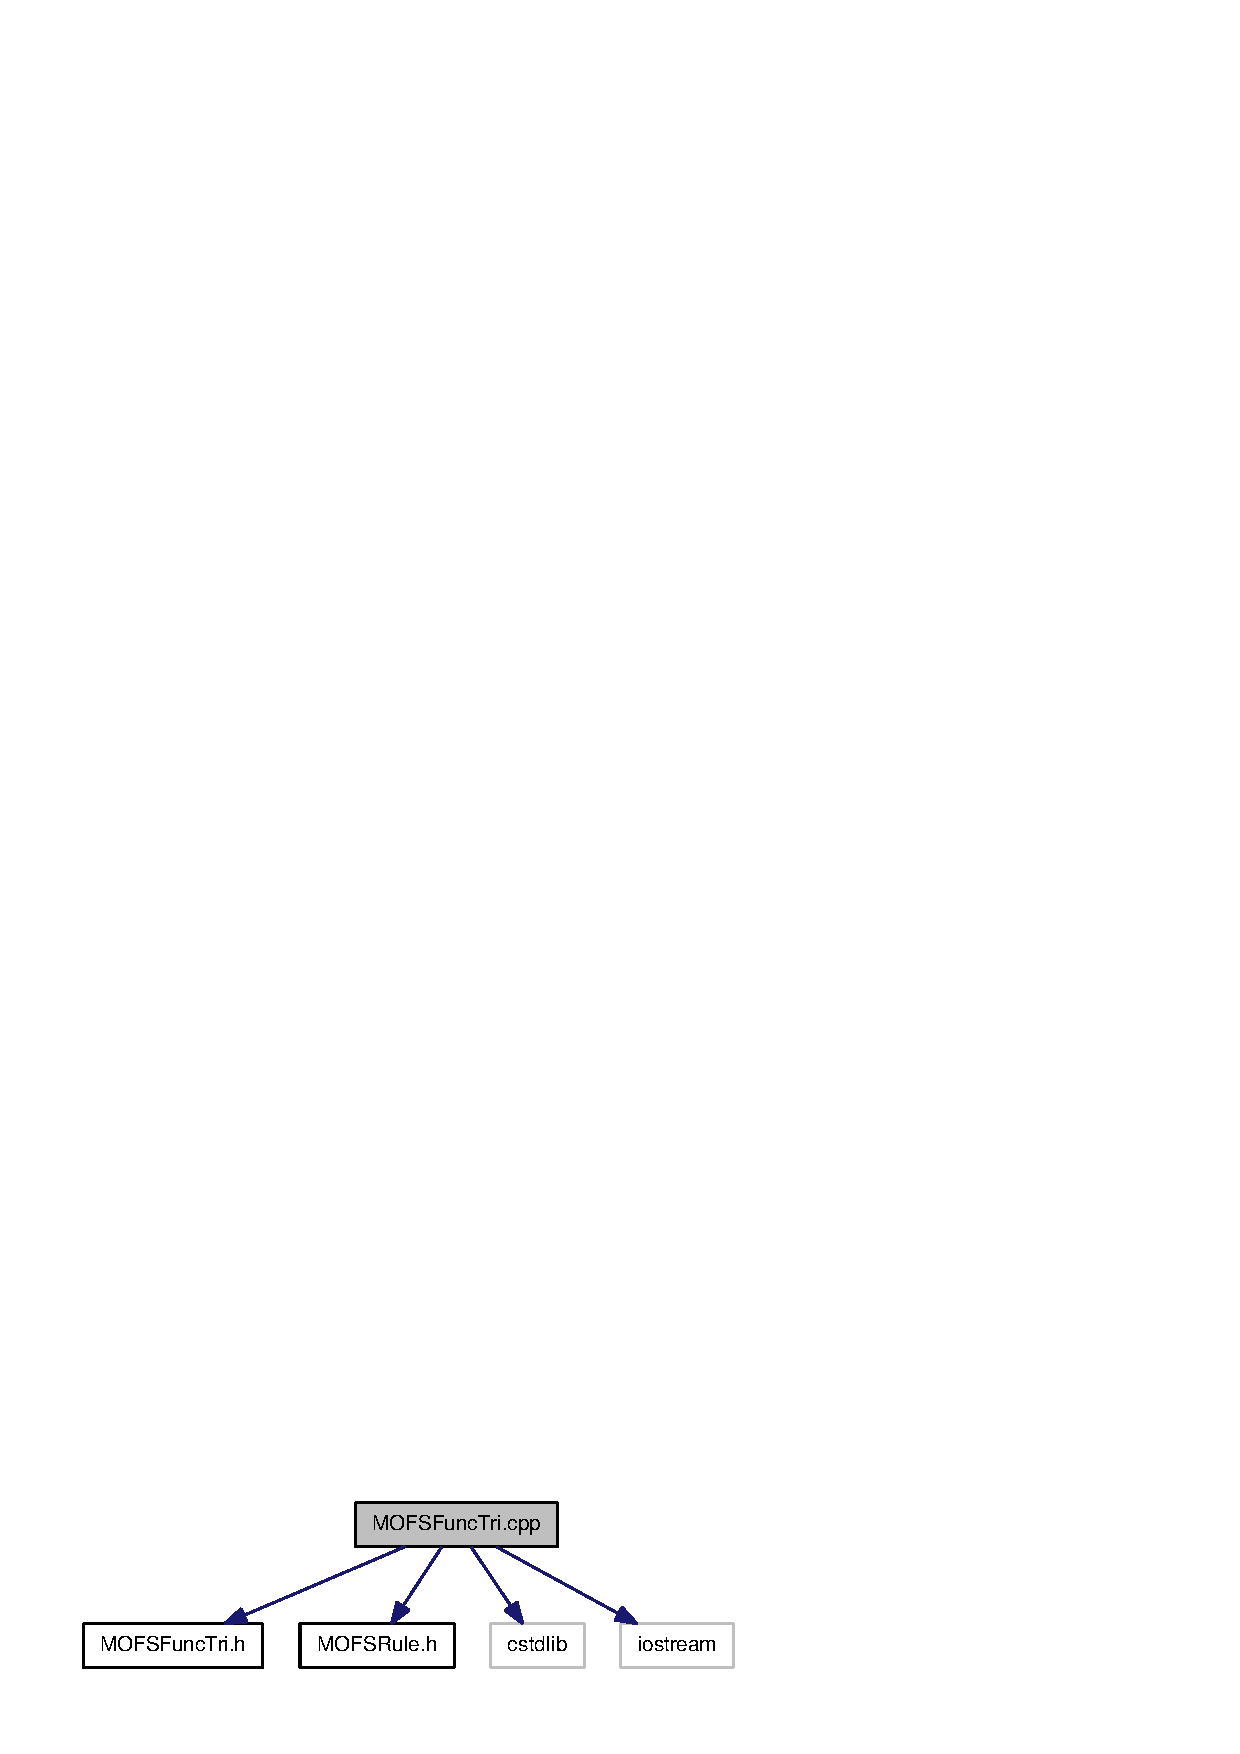
\includegraphics[width=350pt]{MOFSFuncTri_8cpp__incl}
\end{center}
\end{figure}

\section{M\-O\-F\-S\-Func\-Tri.\-h File Reference}
\label{MOFSFuncTri_8h}\index{M\-O\-F\-S\-Func\-Tri.\-h@{M\-O\-F\-S\-Func\-Tri.\-h}}
This graph shows which files directly or indirectly include this file\-:\nopagebreak
\begin{figure}[H]
\begin{center}
\leavevmode
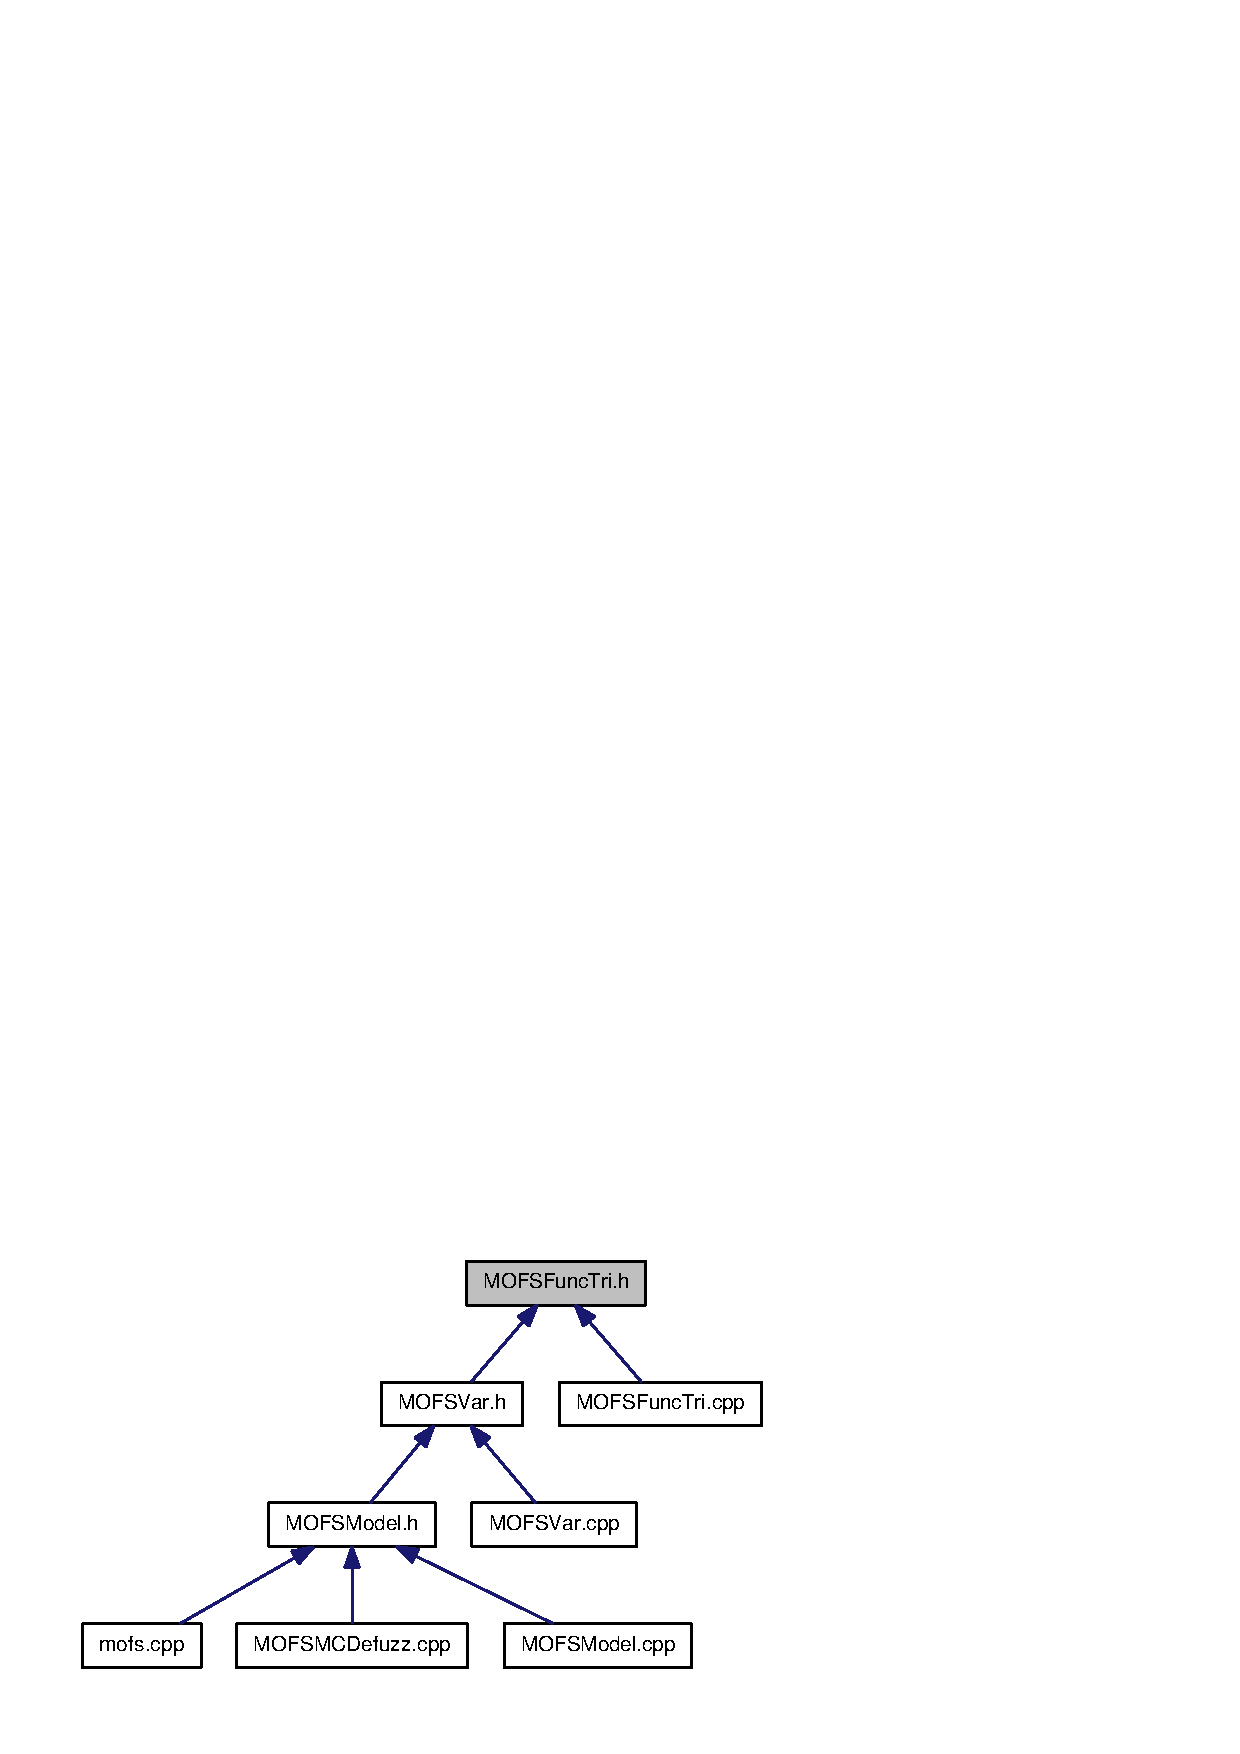
\includegraphics[width=350pt]{MOFSFuncTri_8h__dep__incl}
\end{center}
\end{figure}
\subsection*{Classes}
\begin{DoxyCompactItemize}
\item 
class {\bf M\-O\-F\-S\-Func\-Tri}
\end{DoxyCompactItemize}

\section{M\-O\-F\-S\-M\-C\-Defuzz.\-cpp File Reference}
\label{MOFSMCDefuzz_8cpp}\index{M\-O\-F\-S\-M\-C\-Defuzz.\-cpp@{M\-O\-F\-S\-M\-C\-Defuzz.\-cpp}}
{\ttfamily \#include \char`\"{}M\-O\-F\-S\-Model.\-h\char`\"{}}\\*
{\ttfamily \#include $<$cstdlib$>$}\\*
{\ttfamily \#include $<$iostream$>$}\\*
Include dependency graph for M\-O\-F\-S\-M\-C\-Defuzz.\-cpp\-:\nopagebreak
\begin{figure}[H]
\begin{center}
\leavevmode
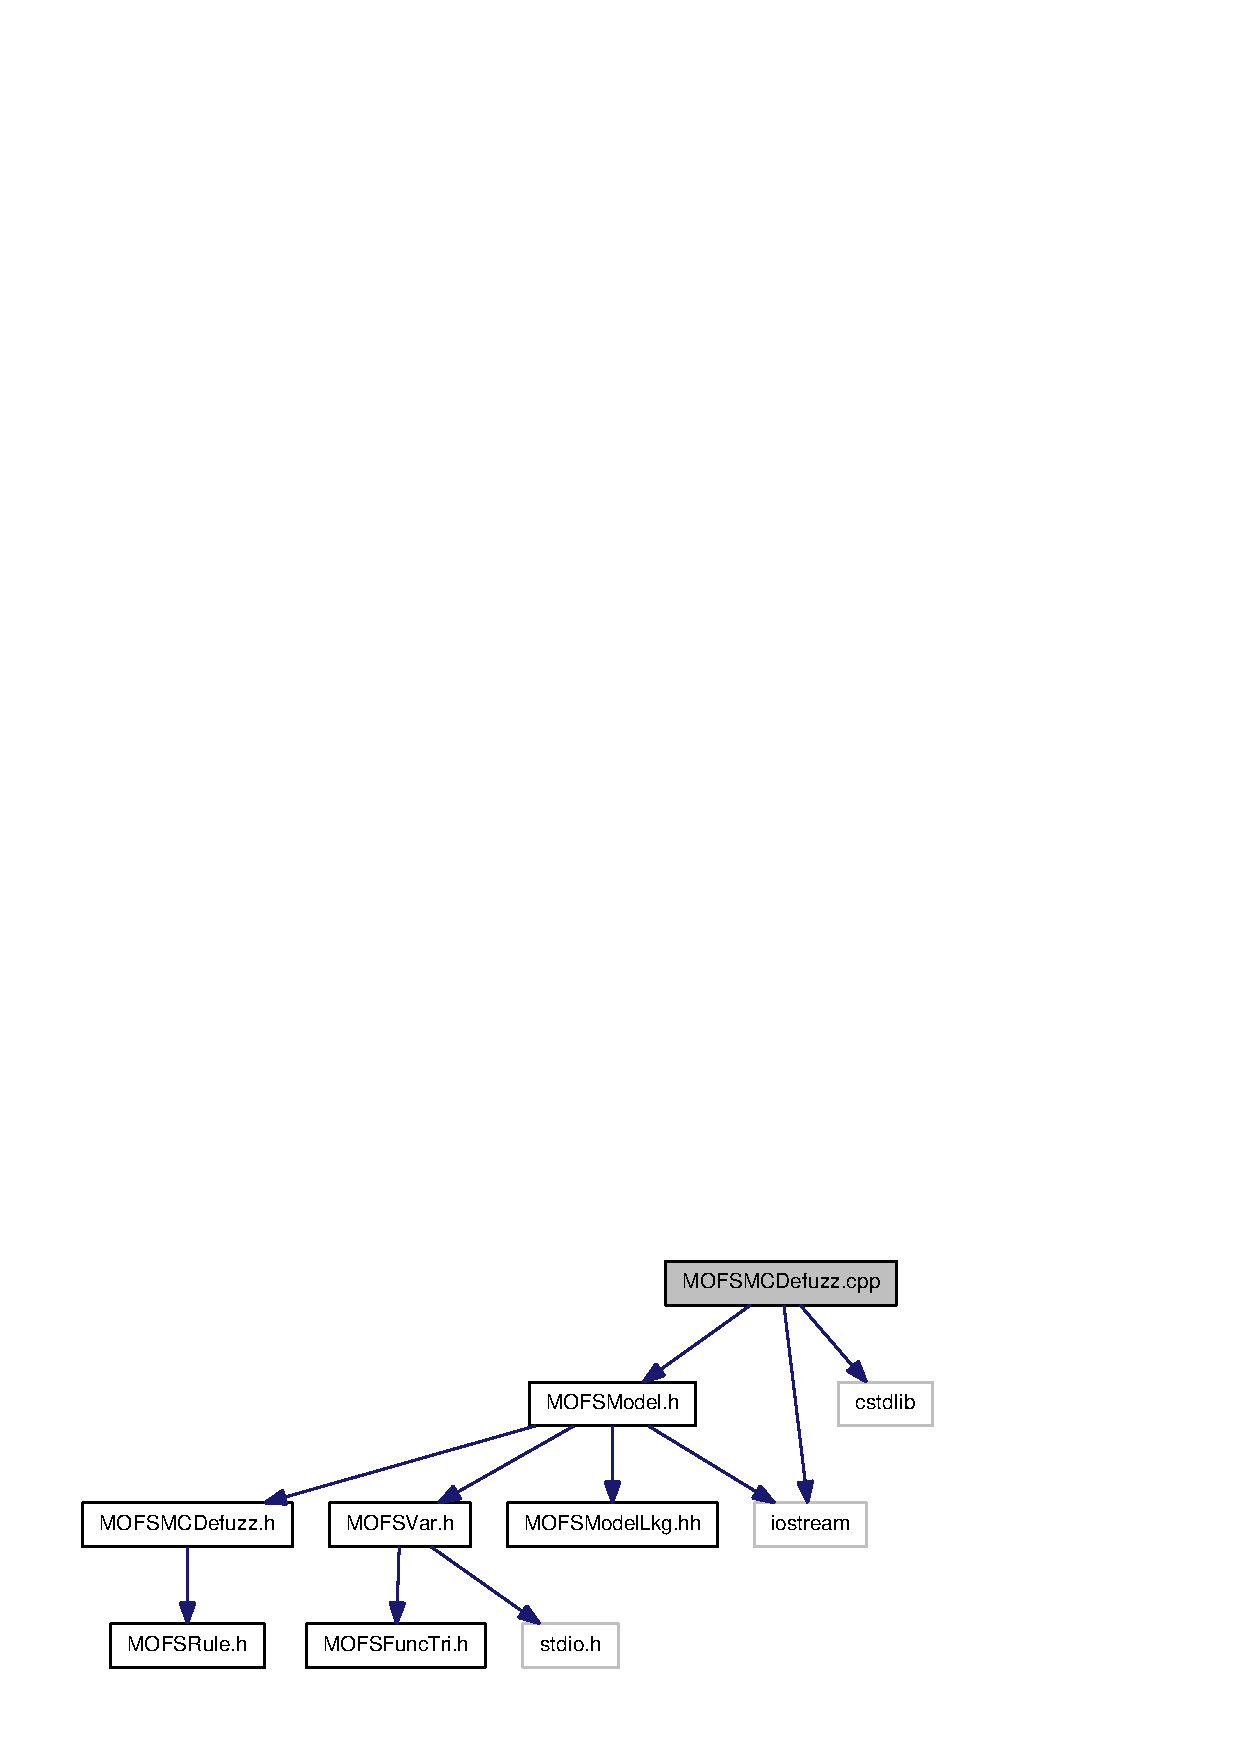
\includegraphics[width=350pt]{MOFSMCDefuzz_8cpp__incl}
\end{center}
\end{figure}
\subsection*{Functions}
\begin{DoxyCompactItemize}
\item 
float {\bf minimus} (float min, float v)
\end{DoxyCompactItemize}


\subsection{Function Documentation}
\index{M\-O\-F\-S\-M\-C\-Defuzz.\-cpp@{M\-O\-F\-S\-M\-C\-Defuzz.\-cpp}!minimus@{minimus}}
\index{minimus@{minimus}!MOFSMCDefuzz.cpp@{M\-O\-F\-S\-M\-C\-Defuzz.\-cpp}}
\subsubsection[{minimus}]{\setlength{\rightskip}{0pt plus 5cm}float minimus (
\begin{DoxyParamCaption}
\item[{float}]{min, }
\item[{float}]{v}
\end{DoxyParamCaption}
)}\label{MOFSMCDefuzz_8cpp_af712f9a80e210af7e2f09ccbe452bb77}


Definition at line 50 of file M\-O\-F\-S\-M\-C\-Defuzz.\-cpp.


\section{M\-O\-F\-S\-M\-C\-Defuzz.\-h File Reference}
\label{MOFSMCDefuzz_8h}\index{M\-O\-F\-S\-M\-C\-Defuzz.\-h@{M\-O\-F\-S\-M\-C\-Defuzz.\-h}}
{\ttfamily \#include \char`\"{}M\-O\-F\-S\-Rule.\-h\char`\"{}}\\*
Include dependency graph for M\-O\-F\-S\-M\-C\-Defuzz.\-h\-:\nopagebreak
\begin{figure}[H]
\begin{center}
\leavevmode
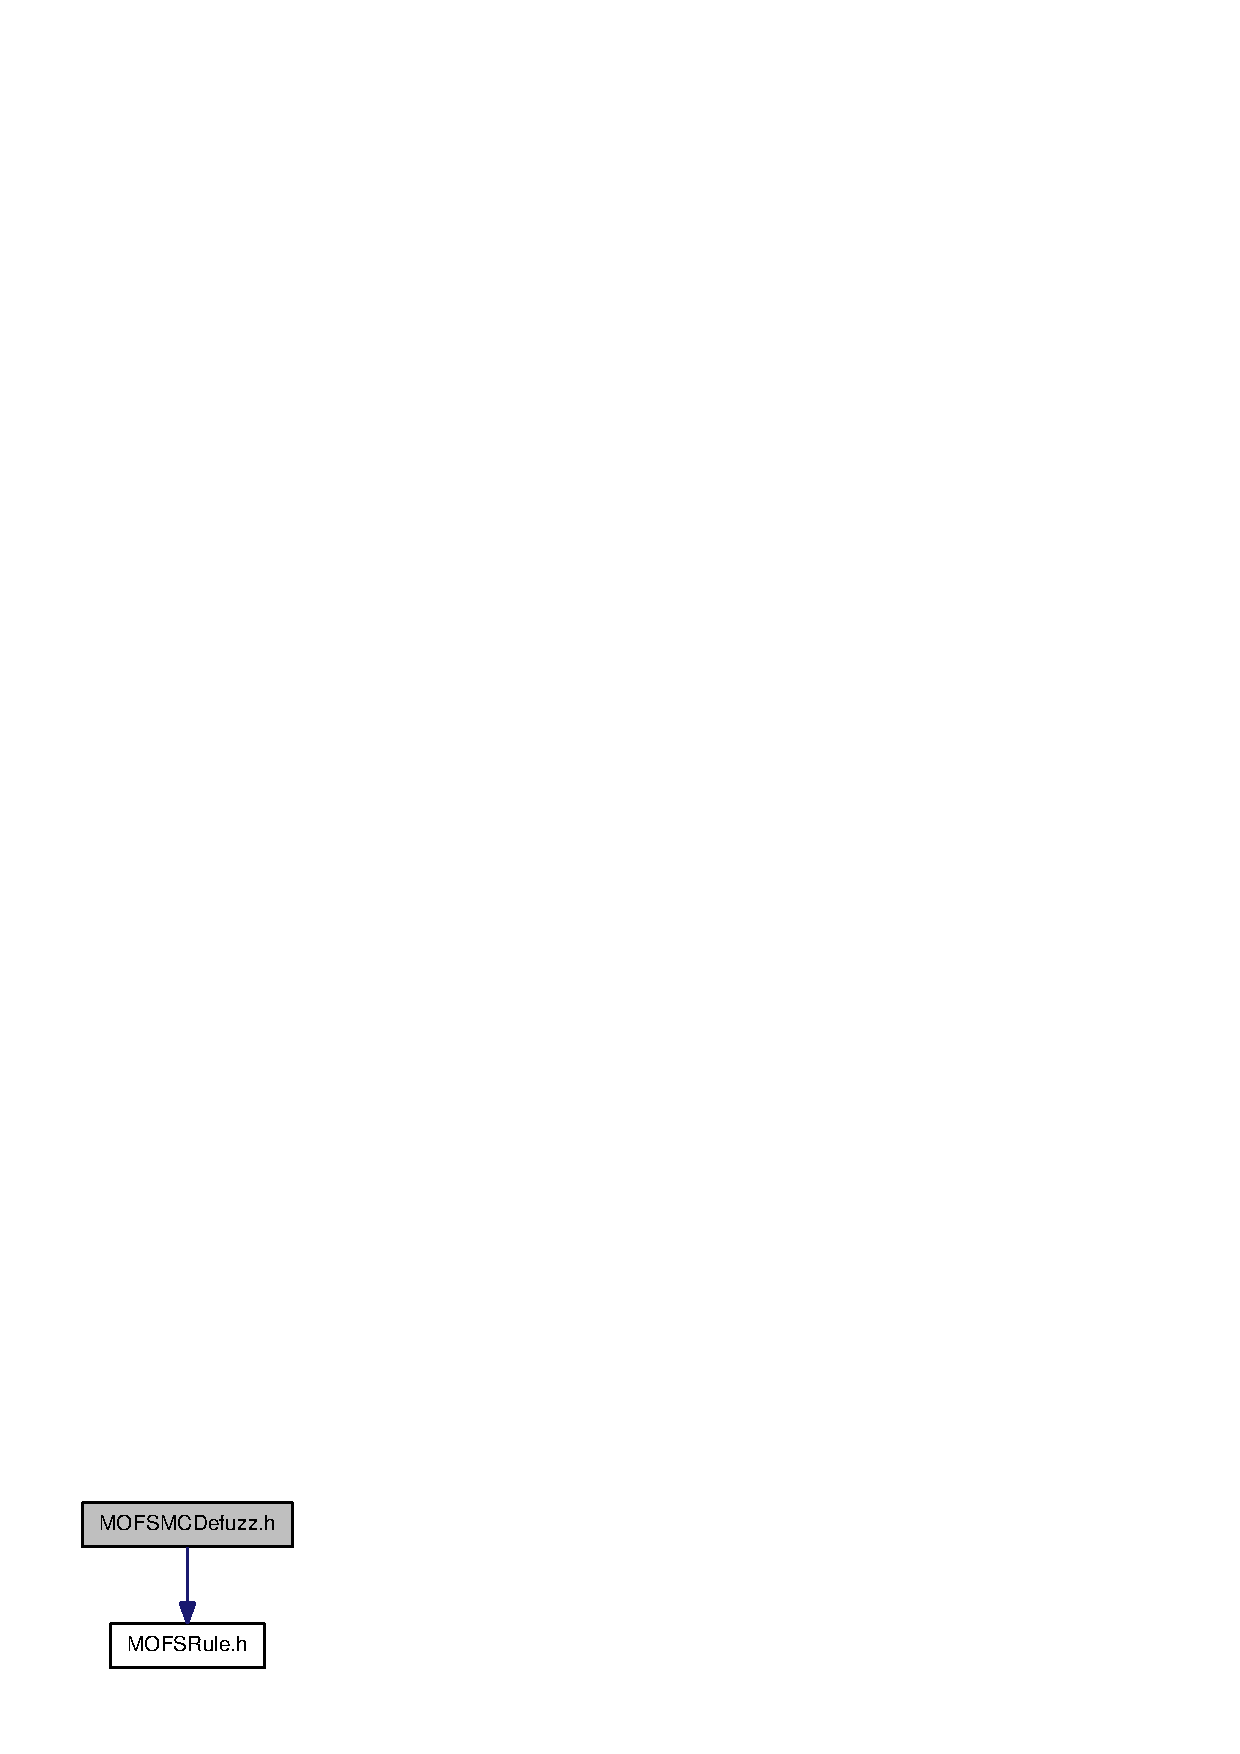
\includegraphics[width=144pt]{MOFSMCDefuzz_8h__incl}
\end{center}
\end{figure}
This graph shows which files directly or indirectly include this file\-:\nopagebreak
\begin{figure}[H]
\begin{center}
\leavevmode
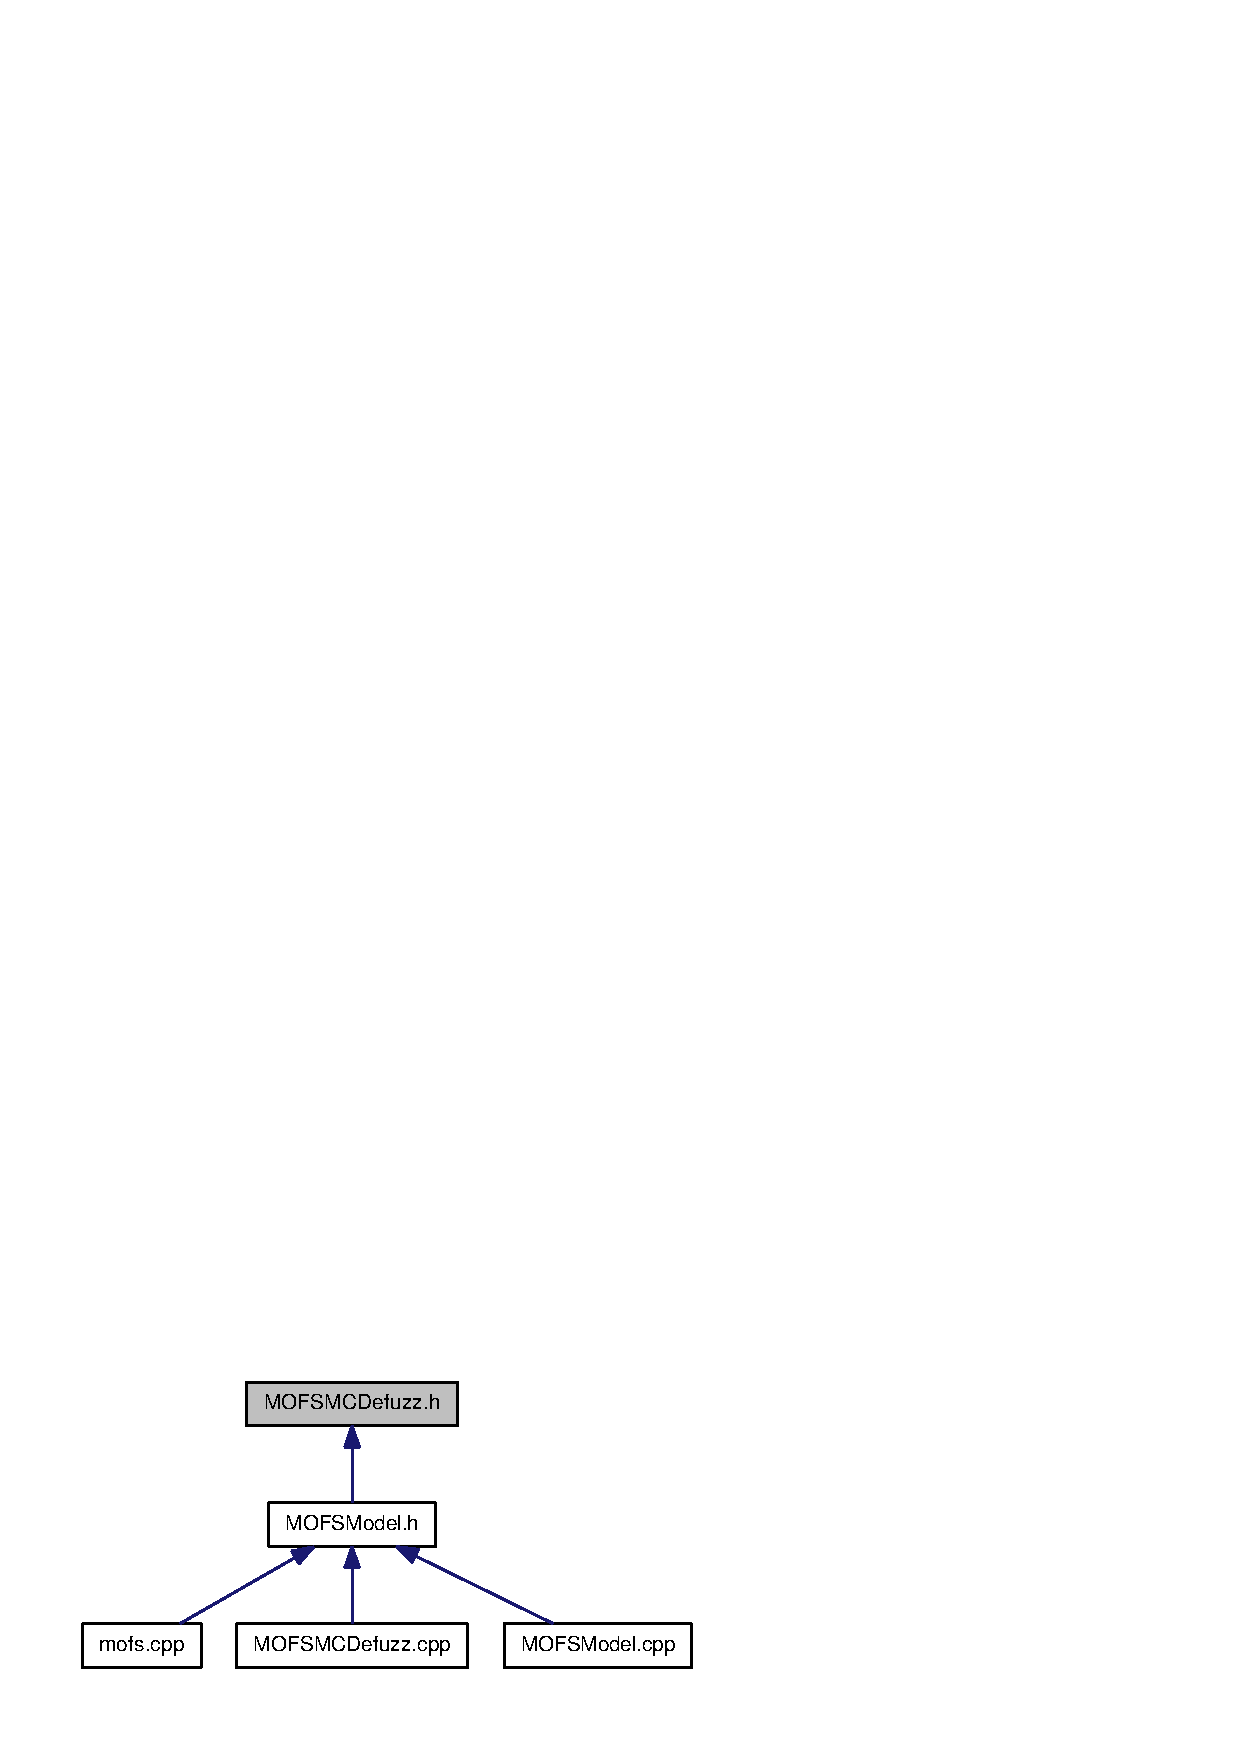
\includegraphics[width=336pt]{MOFSMCDefuzz_8h__dep__incl}
\end{center}
\end{figure}
\subsection*{Classes}
\begin{DoxyCompactItemize}
\item 
class {\bf M\-O\-F\-S\-M\-C\-Defuzz}
\item 
struct {\bf M\-O\-F\-S\-M\-C\-Defuzz\-::\-Rule\-Node}
\end{DoxyCompactItemize}

\section{M\-O\-F\-S\-Model.\-cpp File Reference}
\label{MOFSModel_8cpp}\index{M\-O\-F\-S\-Model.\-cpp@{M\-O\-F\-S\-Model.\-cpp}}
{\ttfamily \#include $<$M\-O\-F\-S\-Model.\-h$>$}\\*
{\ttfamily \#include $<$iostream$>$}\\*
{\ttfamily \#include $<$cstdlib$>$}\\*
{\ttfamily \#include $<$stdlib.\-h$>$}\\*
{\ttfamily \#include $<$string$>$}\\*
Include dependency graph for M\-O\-F\-S\-Model.\-cpp\-:\nopagebreak
\begin{figure}[H]
\begin{center}
\leavevmode
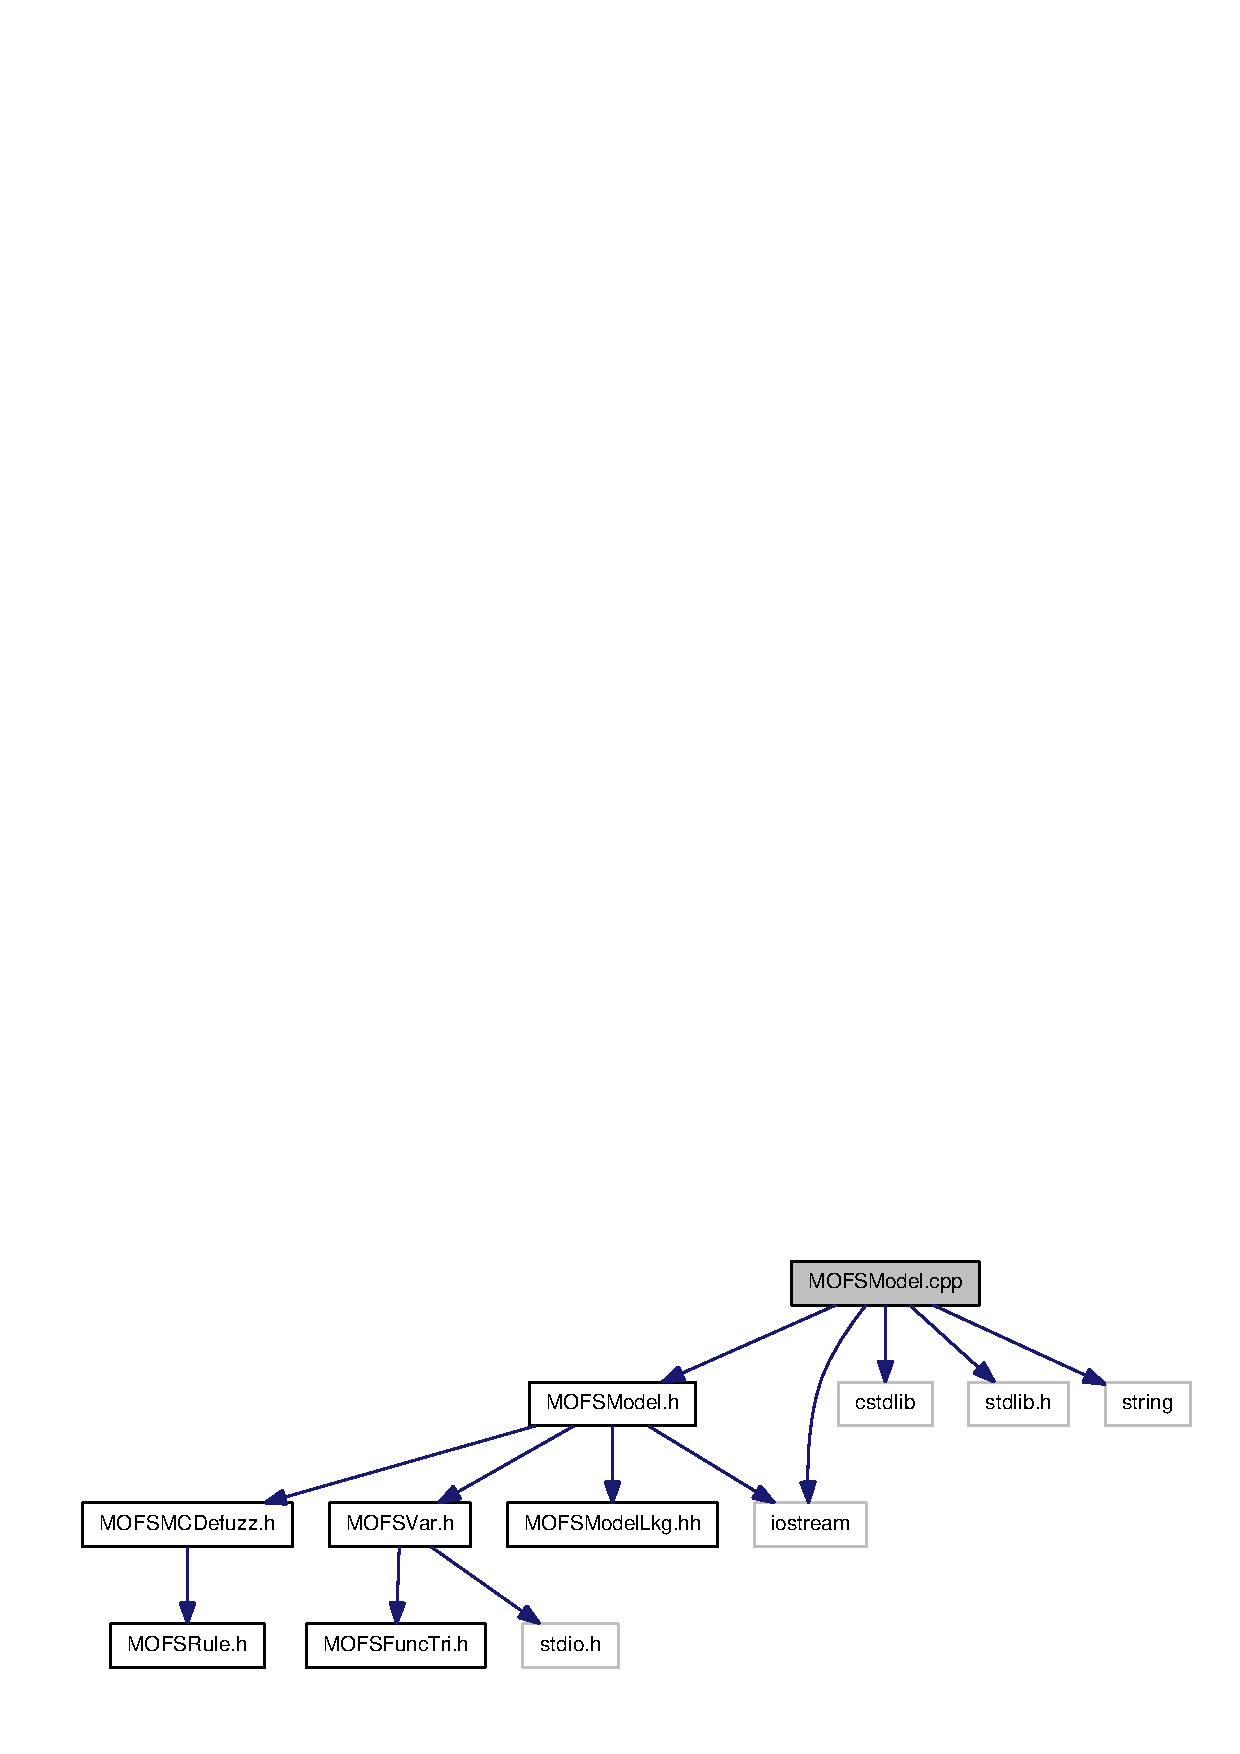
\includegraphics[width=350pt]{MOFSModel_8cpp__incl}
\end{center}
\end{figure}

\section{M\-O\-F\-S\-Model.\-h File Reference}
\label{MOFSModel_8h}\index{M\-O\-F\-S\-Model.\-h@{M\-O\-F\-S\-Model.\-h}}
{\ttfamily \#include \char`\"{}M\-O\-F\-S\-M\-C\-Defuzz.\-h\char`\"{}}\\*
{\ttfamily \#include \char`\"{}M\-O\-F\-S\-Var.\-h\char`\"{}}\\*
{\ttfamily \#include \char`\"{}M\-O\-F\-S\-Model\-Lkg.\-hh\char`\"{}}\\*
{\ttfamily \#include $<$iostream$>$}\\*
Include dependency graph for M\-O\-F\-S\-Model.\-h\-:\nopagebreak
\begin{figure}[H]
\begin{center}
\leavevmode
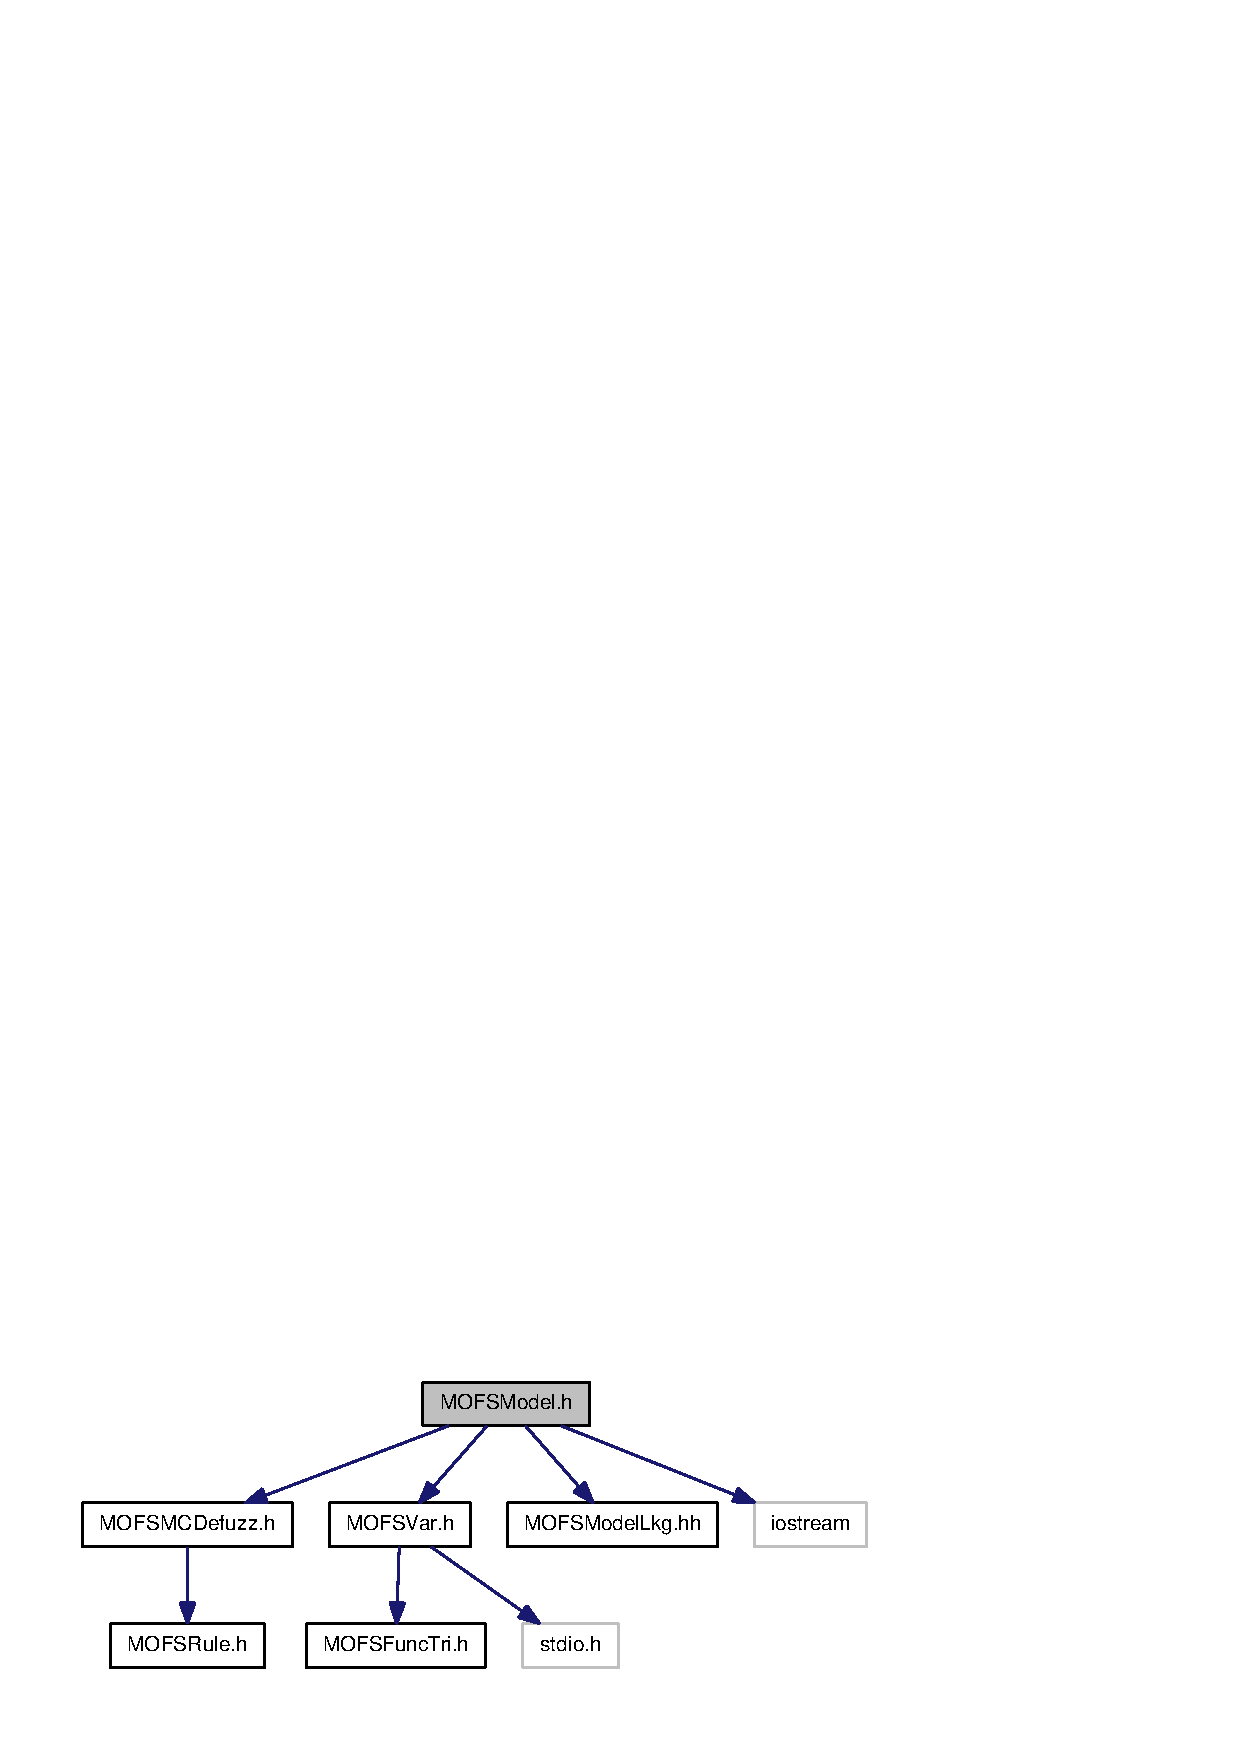
\includegraphics[width=350pt]{MOFSModel_8h__incl}
\end{center}
\end{figure}
This graph shows which files directly or indirectly include this file\-:\nopagebreak
\begin{figure}[H]
\begin{center}
\leavevmode
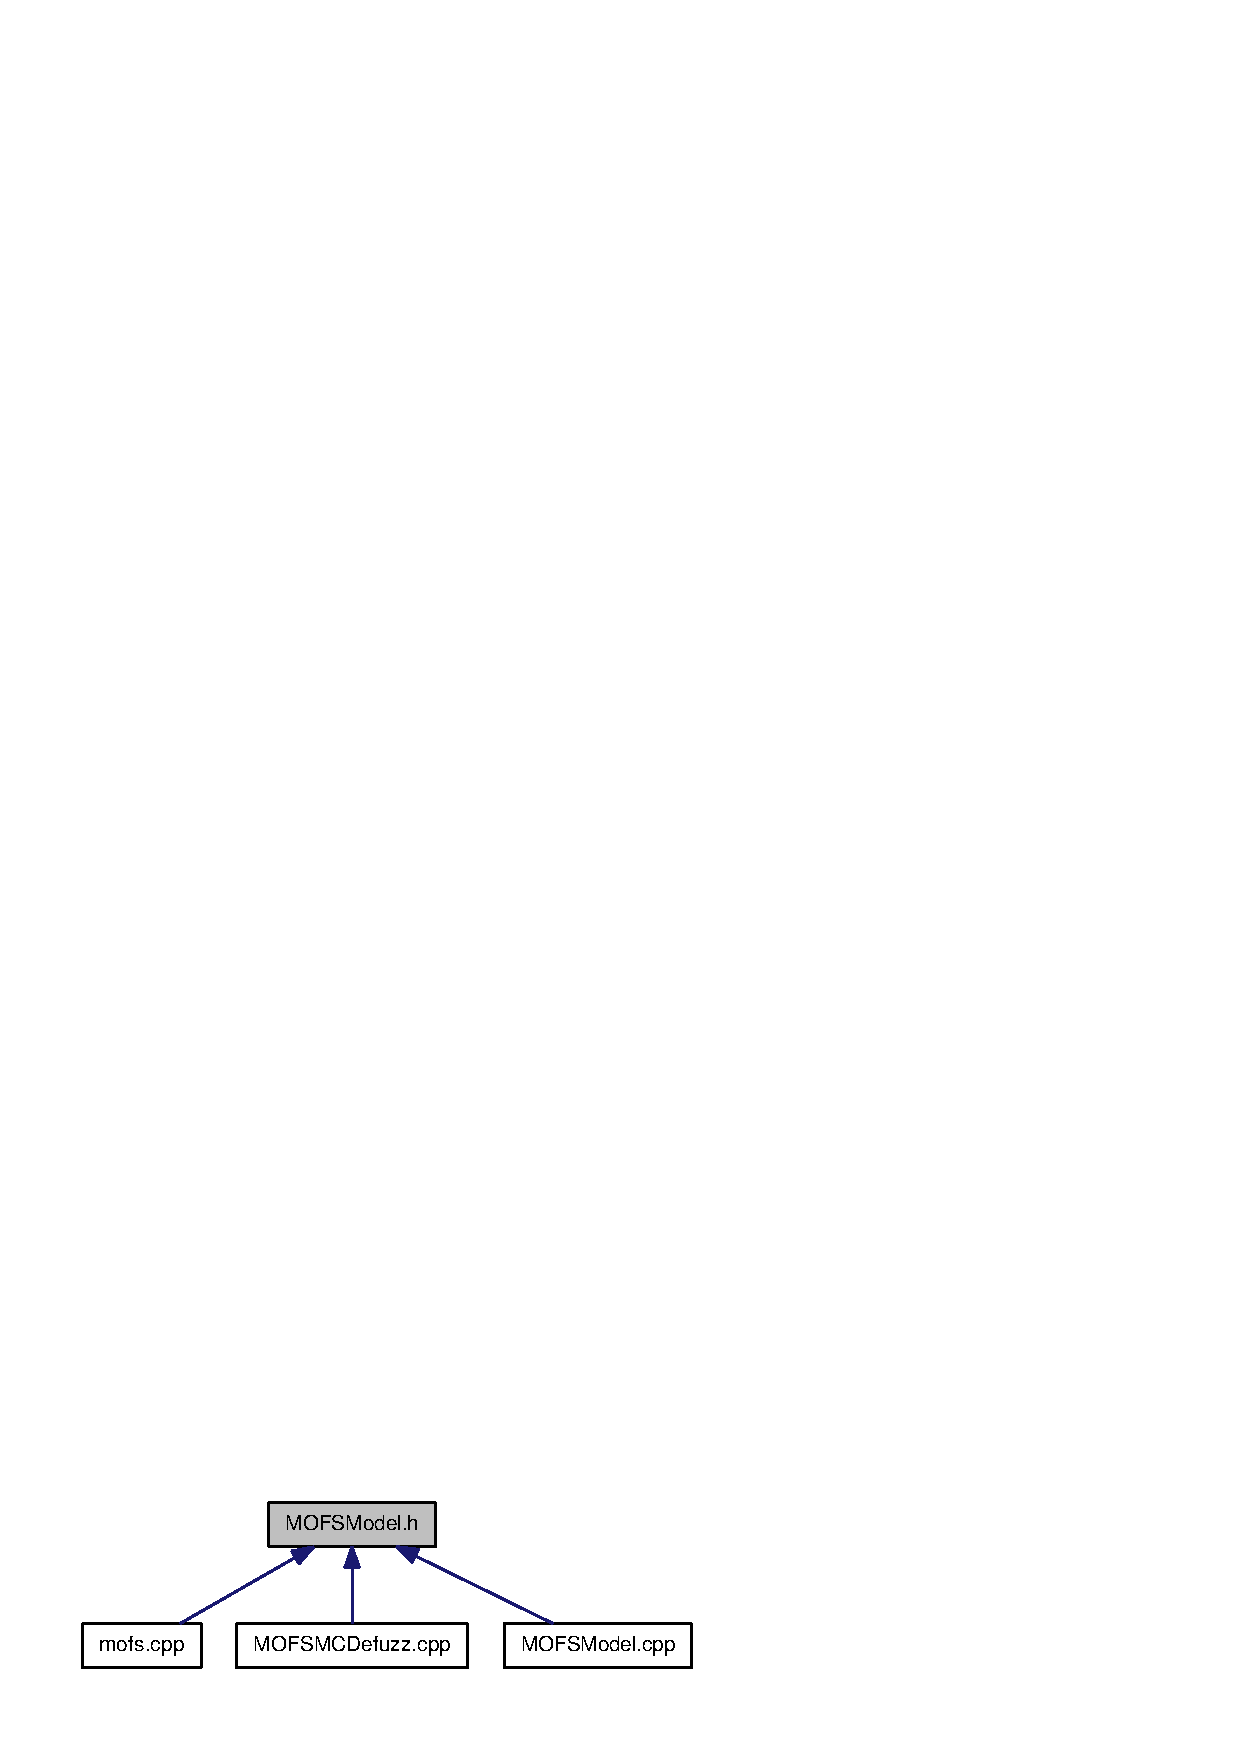
\includegraphics[width=336pt]{MOFSModel_8h__dep__incl}
\end{center}
\end{figure}
\subsection*{Classes}
\begin{DoxyCompactItemize}
\item 
class {\bf mofs\-::\-M\-O\-F\-S\-Model}
\item 
struct {\bf mofs\-::\-Output}
\item 
struct {\bf mofs\-::\-Rule\-Data}
\item 
struct {\bf mofs\-::\-Rule\-Node}
\item 
struct {\bf mofs\-::\-Rule\-Values}
\item 
struct {\bf mofs\-::\-Set}
\item 
struct {\bf mofs\-::\-Vars\-Node}
\end{DoxyCompactItemize}
\subsection*{Namespaces}
\begin{DoxyCompactItemize}
\item 
{\bf mofs}
\end{DoxyCompactItemize}
\subsection*{Typedefs}
\begin{DoxyCompactItemize}
\item 
typedef float {\bf mofs\-::\-Inputs} [$\,$]
\end{DoxyCompactItemize}

\section{M\-O\-F\-S\-Model\-Lkg.\-hh File Reference}
\label{MOFSModelLkg_8hh}\index{M\-O\-F\-S\-Model\-Lkg.\-hh@{M\-O\-F\-S\-Model\-Lkg.\-hh}}
This graph shows which files directly or indirectly include this file\-:\nopagebreak
\begin{figure}[H]
\begin{center}
\leavevmode
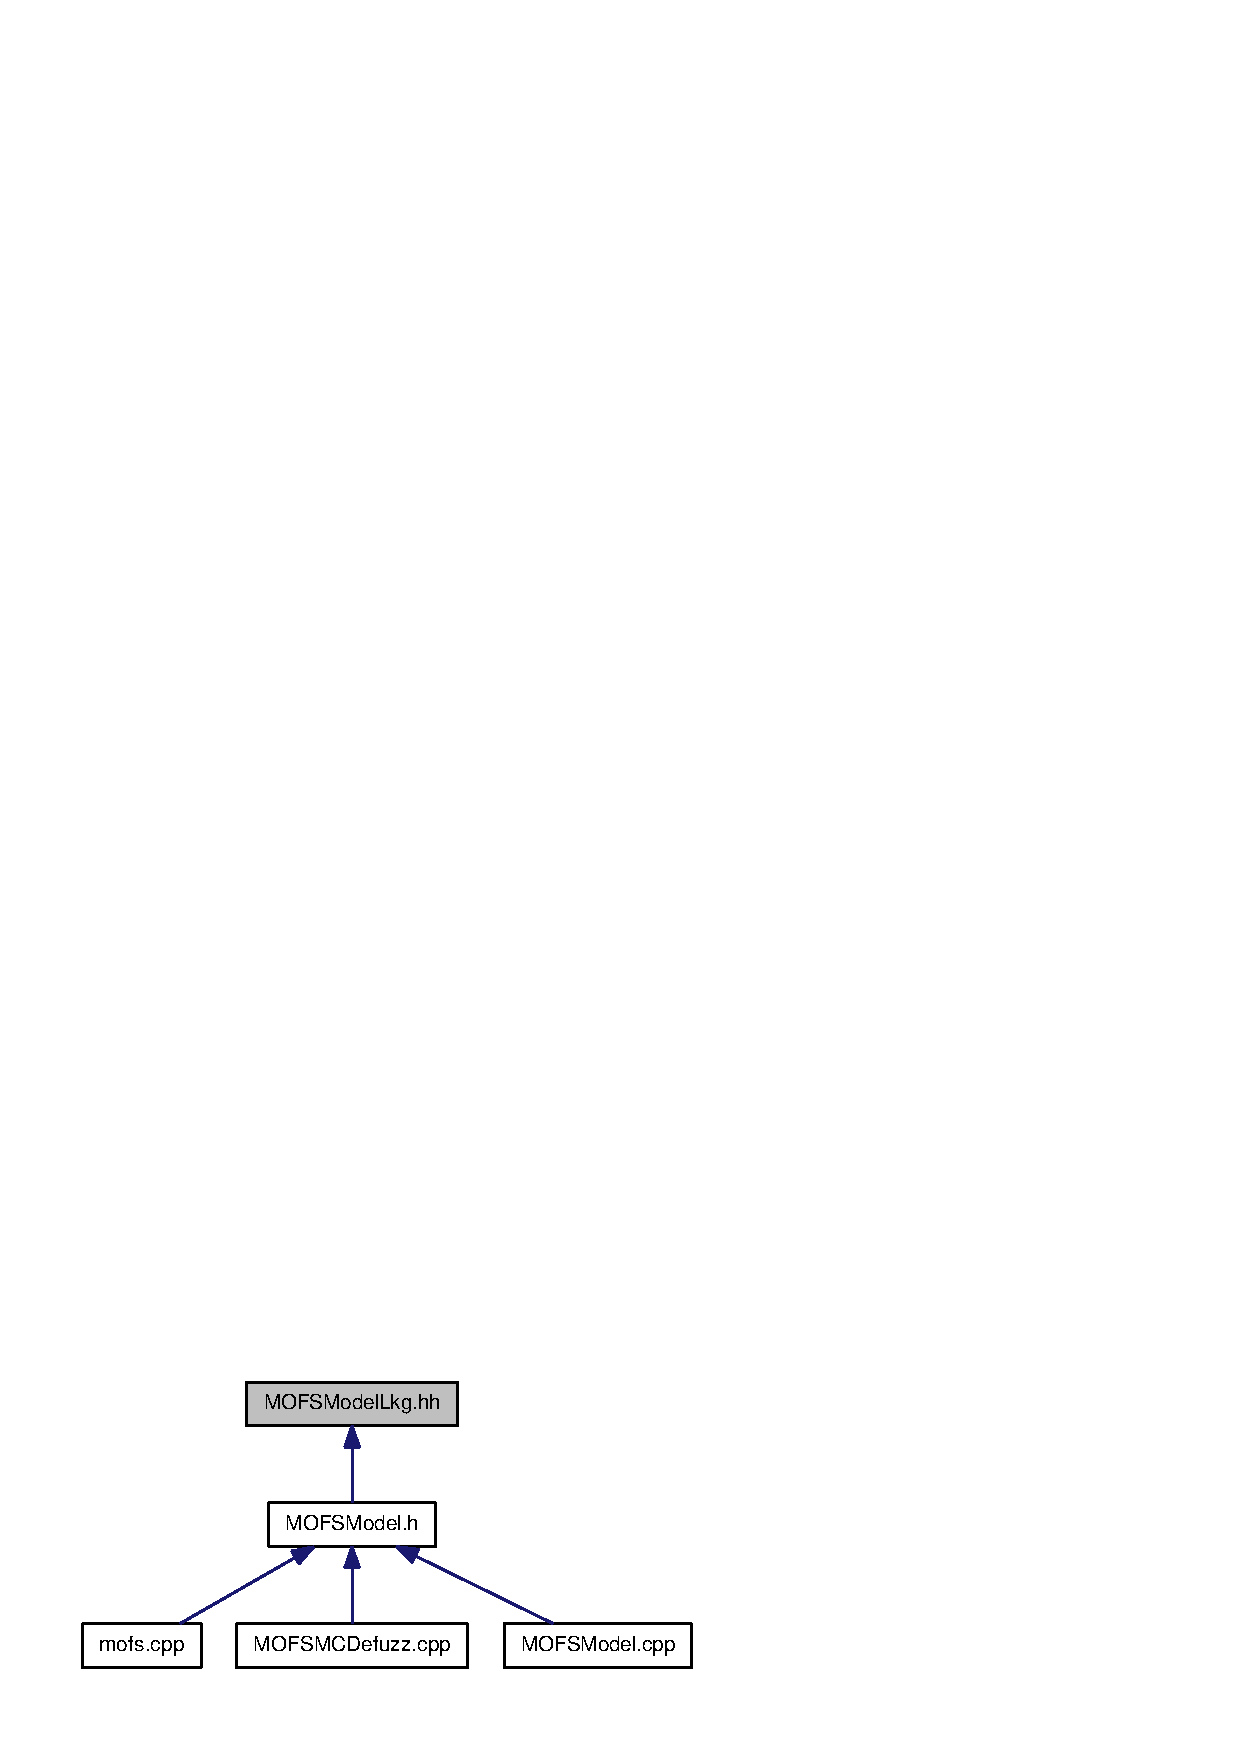
\includegraphics[width=336pt]{MOFSModelLkg_8hh__dep__incl}
\end{center}
\end{figure}
\subsection*{Functions}
\begin{DoxyCompactItemize}
\item 
float {\bf input\-Irq} (float inputs[$\,$], float $\ast$\-\_\-output)
\item 
void {\bf M\-O\-F\-S\-Model} (char $\ast$file, int \-\_\-mode)
\end{DoxyCompactItemize}


\subsection{Function Documentation}
\index{M\-O\-F\-S\-Model\-Lkg.\-hh@{M\-O\-F\-S\-Model\-Lkg.\-hh}!input\-Irq@{input\-Irq}}
\index{input\-Irq@{input\-Irq}!MOFSModelLkg.hh@{M\-O\-F\-S\-Model\-Lkg.\-hh}}
\subsubsection[{input\-Irq}]{\setlength{\rightskip}{0pt plus 5cm}float input\-Irq (
\begin{DoxyParamCaption}
\item[{float}]{inputs[$\,$], }
\item[{float $\ast$}]{\-\_\-output}
\end{DoxyParamCaption}
)}\label{MOFSModelLkg_8hh_ac6ad1ed6b116306dfc98b66801db3787}
\index{M\-O\-F\-S\-Model\-Lkg.\-hh@{M\-O\-F\-S\-Model\-Lkg.\-hh}!M\-O\-F\-S\-Model@{M\-O\-F\-S\-Model}}
\index{M\-O\-F\-S\-Model@{M\-O\-F\-S\-Model}!MOFSModelLkg.hh@{M\-O\-F\-S\-Model\-Lkg.\-hh}}
\subsubsection[{M\-O\-F\-S\-Model}]{\setlength{\rightskip}{0pt plus 5cm}void M\-O\-F\-S\-Model (
\begin{DoxyParamCaption}
\item[{char $\ast$}]{file, }
\item[{int}]{\-\_\-mode}
\end{DoxyParamCaption}
)}\label{MOFSModelLkg_8hh_a3a0709df4b3dd762042f8d849b2c6571}

\section{M\-O\-F\-S\-Rule.\-cpp File Reference}
\label{MOFSRule_8cpp}\index{M\-O\-F\-S\-Rule.\-cpp@{M\-O\-F\-S\-Rule.\-cpp}}
{\ttfamily \#include $<$string$>$}\\*
{\ttfamily \#include $<$iostream$>$}\\*
{\ttfamily \#include $<$cstdlib$>$}\\*
{\ttfamily \#include $<$stdlib.\-h$>$}\\*
{\ttfamily \#include $<$stdio.\-h$>$}\\*
{\ttfamily \#include \char`\"{}M\-O\-F\-S\-Rule.\-h\char`\"{}}\\*
Include dependency graph for M\-O\-F\-S\-Rule.\-cpp\-:\nopagebreak
\begin{figure}[H]
\begin{center}
\leavevmode
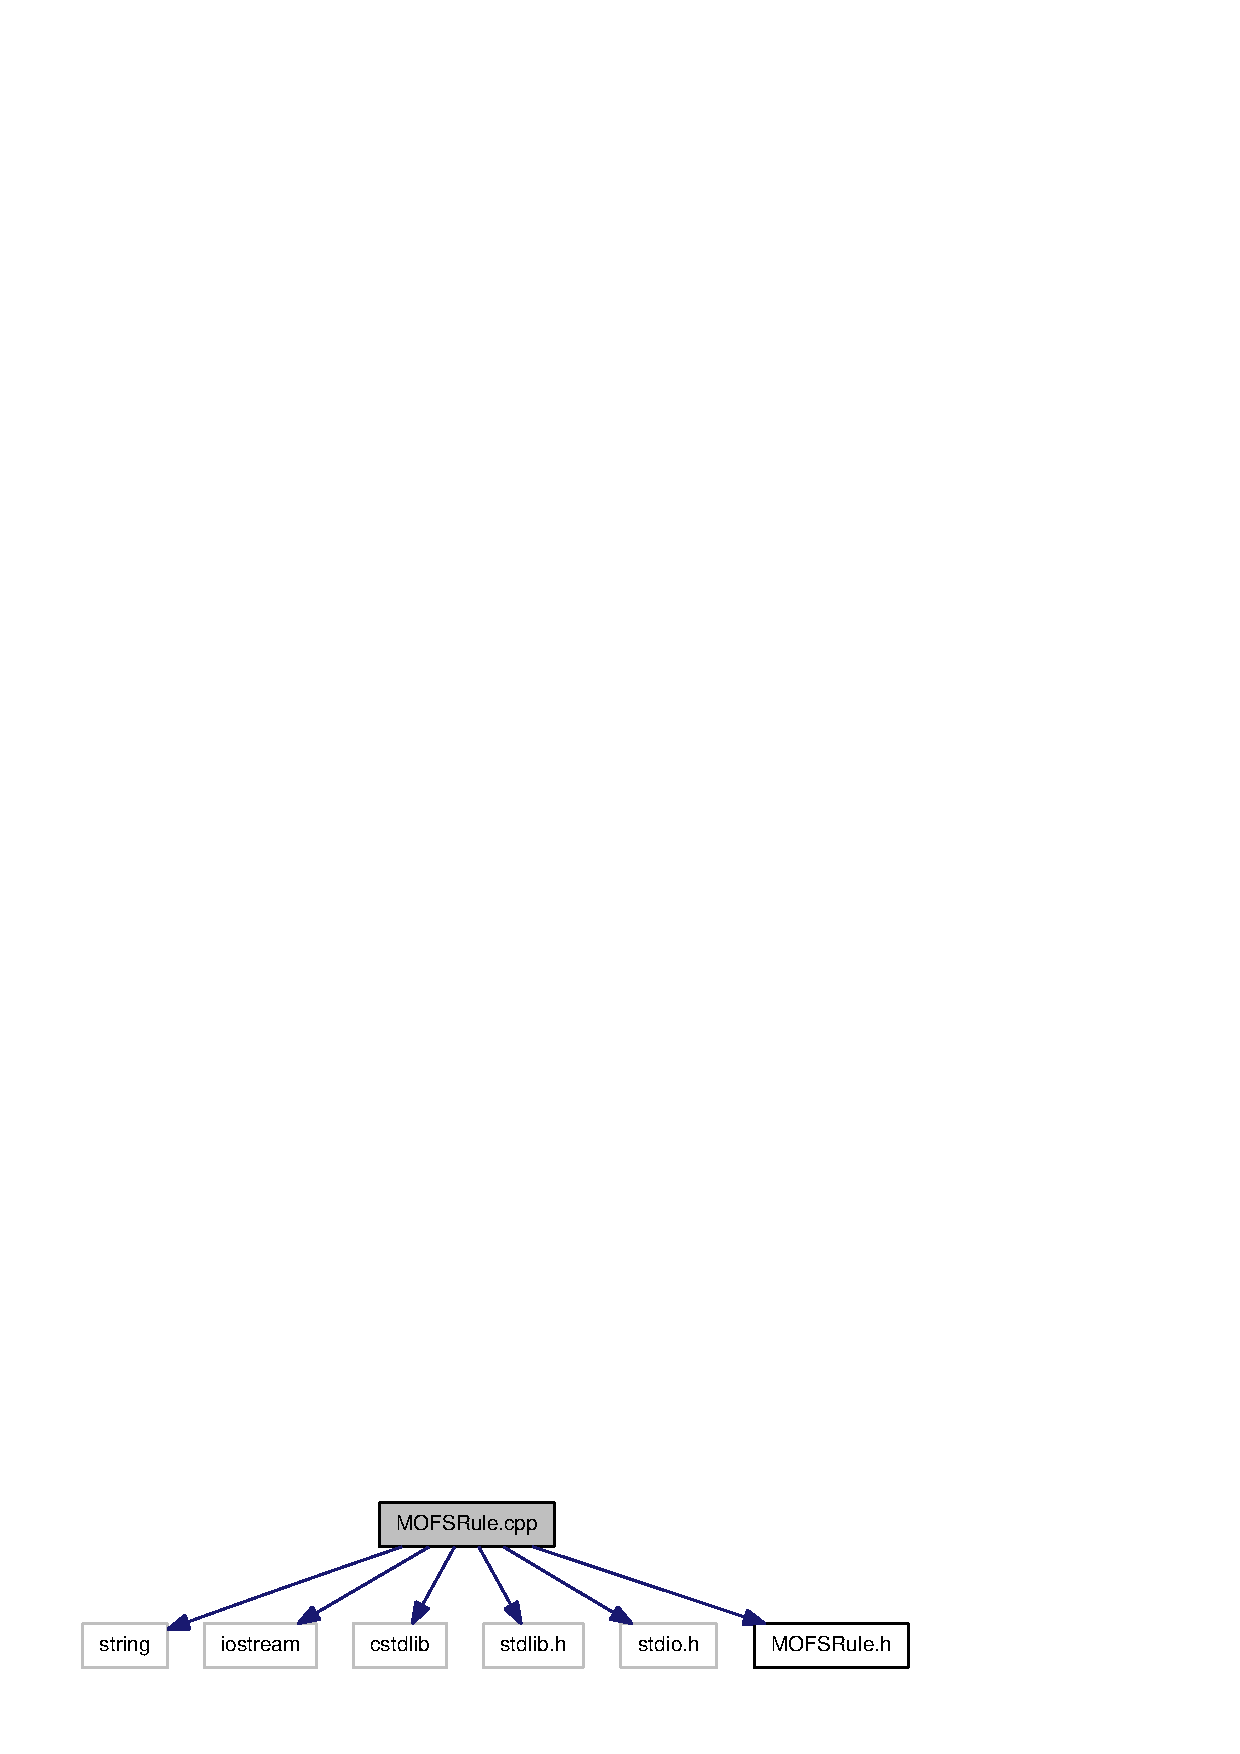
\includegraphics[width=350pt]{MOFSRule_8cpp__incl}
\end{center}
\end{figure}

\section{M\-O\-F\-S\-Rule.\-h File Reference}
\label{MOFSRule_8h}\index{M\-O\-F\-S\-Rule.\-h@{M\-O\-F\-S\-Rule.\-h}}
This graph shows which files directly or indirectly include this file\-:\nopagebreak
\begin{figure}[H]
\begin{center}
\leavevmode
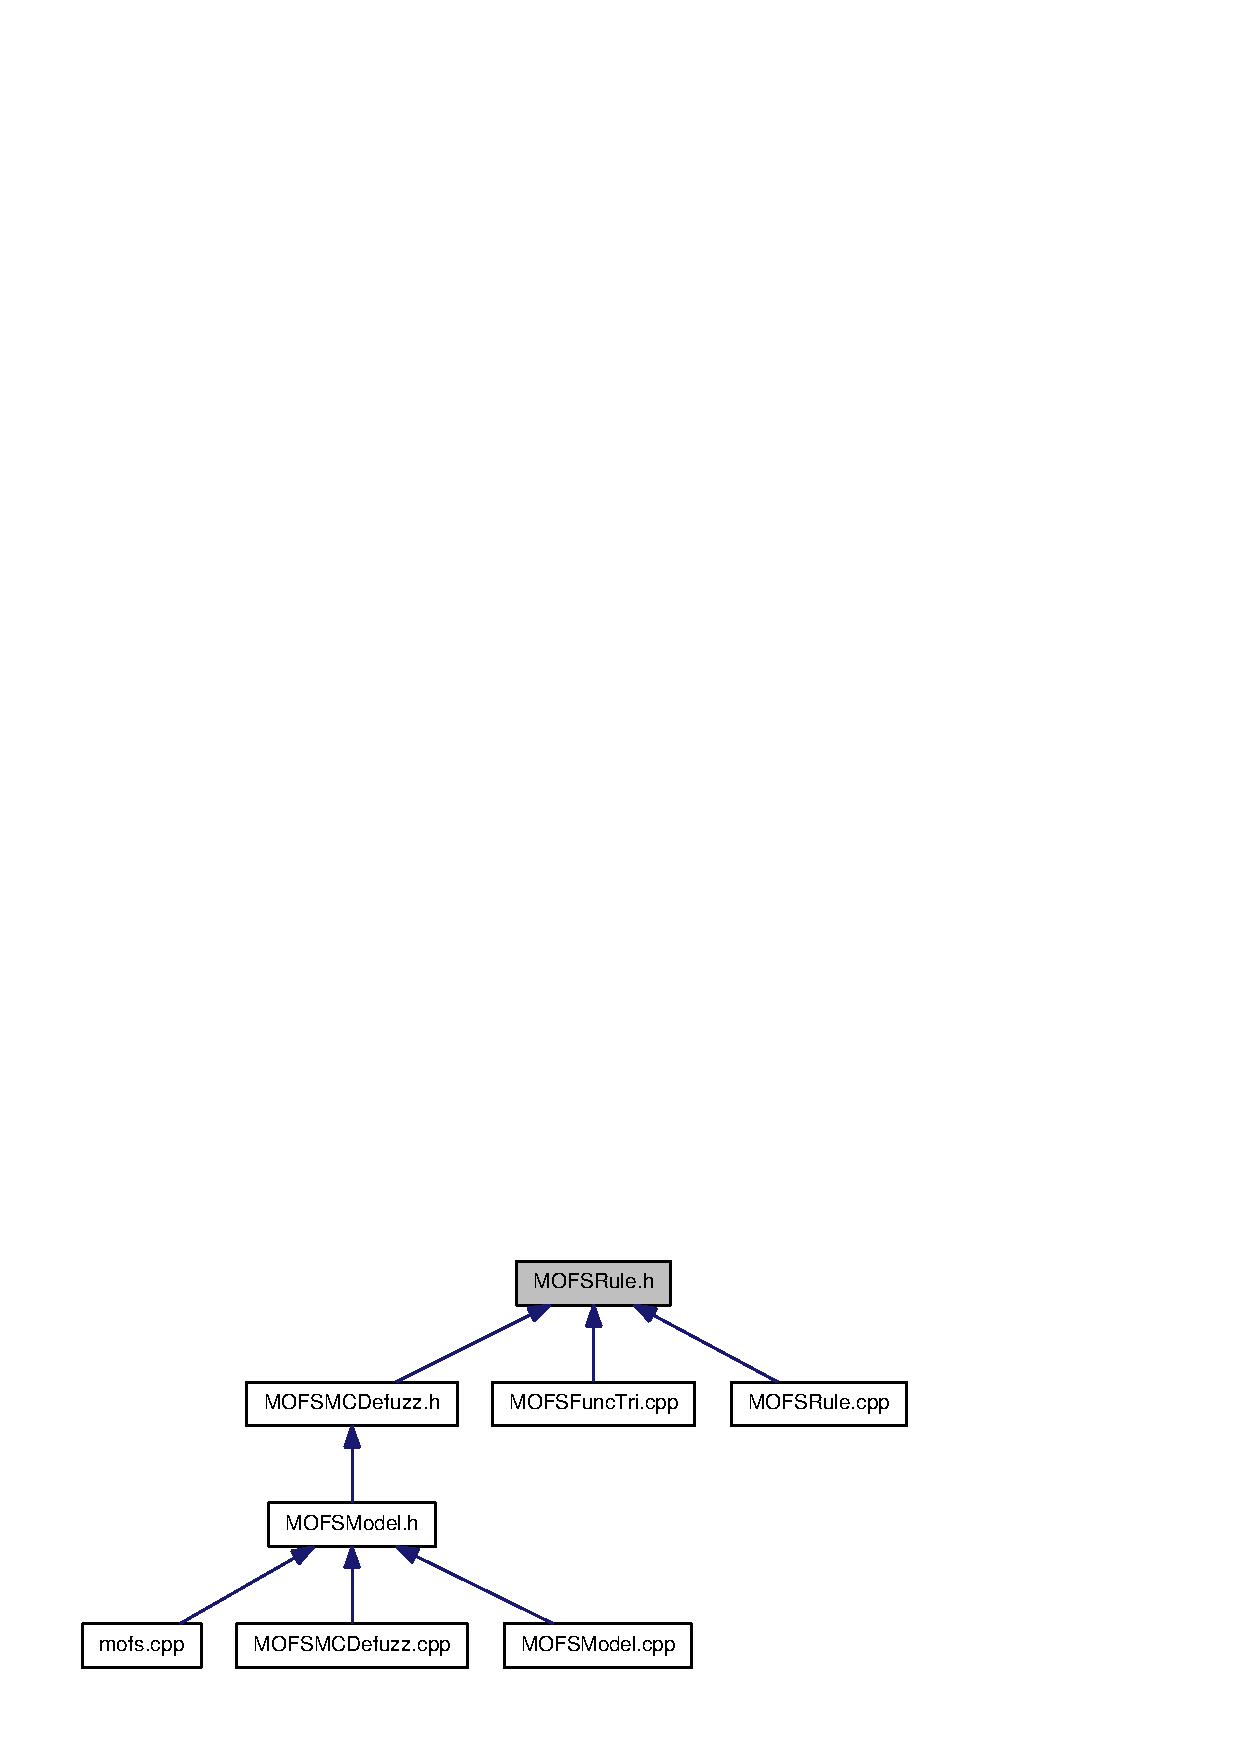
\includegraphics[width=350pt]{MOFSRule_8h__dep__incl}
\end{center}
\end{figure}
\subsection*{Classes}
\begin{DoxyCompactItemize}
\item 
class {\bf M\-O\-F\-S\-Rule}
\item 
struct {\bf M\-O\-F\-S\-Rule\-::\-Set}
\end{DoxyCompactItemize}

\section{M\-O\-F\-S\-Var.\-cpp File Reference}
\label{MOFSVar_8cpp}\index{M\-O\-F\-S\-Var.\-cpp@{M\-O\-F\-S\-Var.\-cpp}}
{\ttfamily \#include \char`\"{}M\-O\-F\-S\-Var.\-h\char`\"{}}\\*
{\ttfamily \#include $<$cstdlib$>$}\\*
{\ttfamily \#include $<$iostream$>$}\\*
{\ttfamily \#include $<$stdio.\-h$>$}\\*
{\ttfamily \#include $<$string.\-h$>$}\\*
Include dependency graph for M\-O\-F\-S\-Var.\-cpp\-:\nopagebreak
\begin{figure}[H]
\begin{center}
\leavevmode
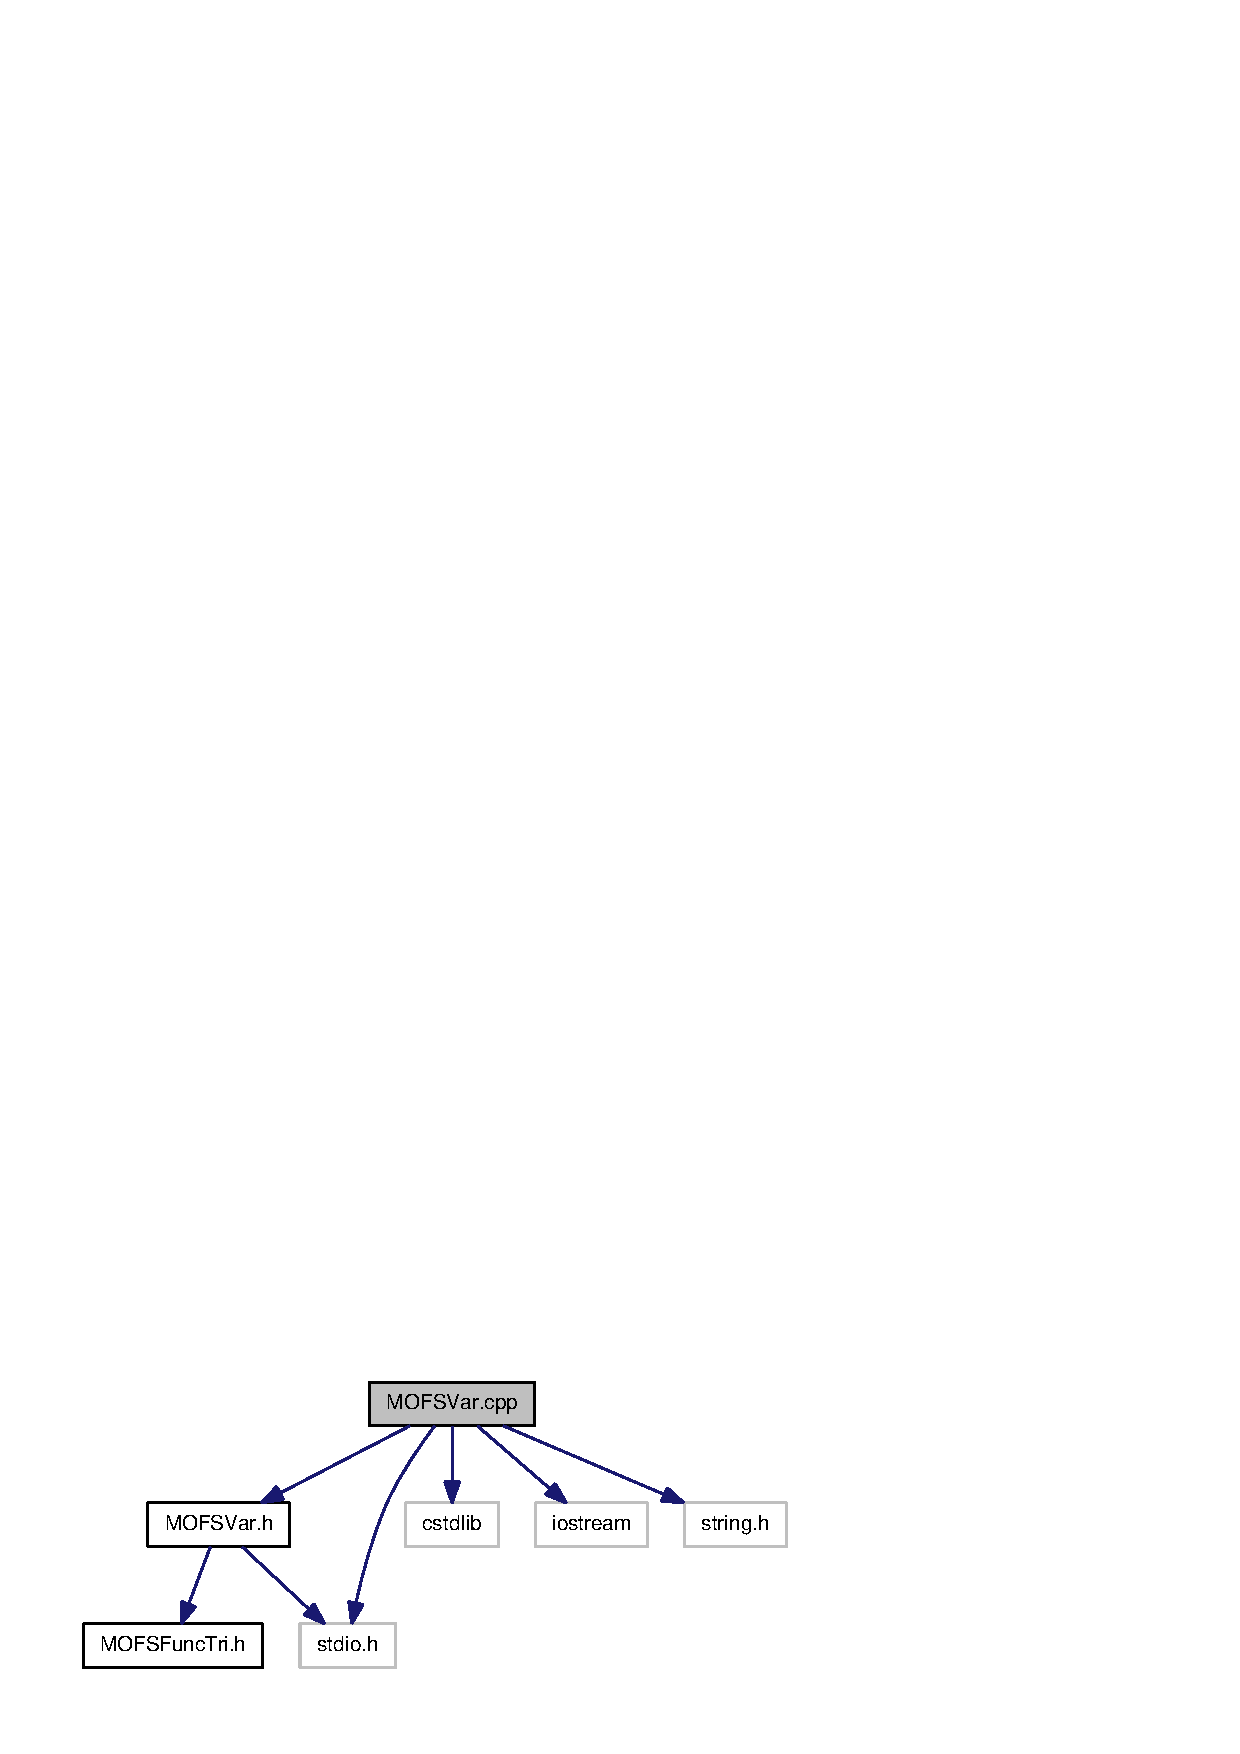
\includegraphics[width=350pt]{MOFSVar_8cpp__incl}
\end{center}
\end{figure}

\section{M\-O\-F\-S\-Var.\-h File Reference}
\label{MOFSVar_8h}\index{M\-O\-F\-S\-Var.\-h@{M\-O\-F\-S\-Var.\-h}}
{\ttfamily \#include \char`\"{}M\-O\-F\-S\-Func\-Tri.\-h\char`\"{}}\\*
{\ttfamily \#include $<$stdio.\-h$>$}\\*
Include dependency graph for M\-O\-F\-S\-Var.\-h\-:\nopagebreak
\begin{figure}[H]
\begin{center}
\leavevmode
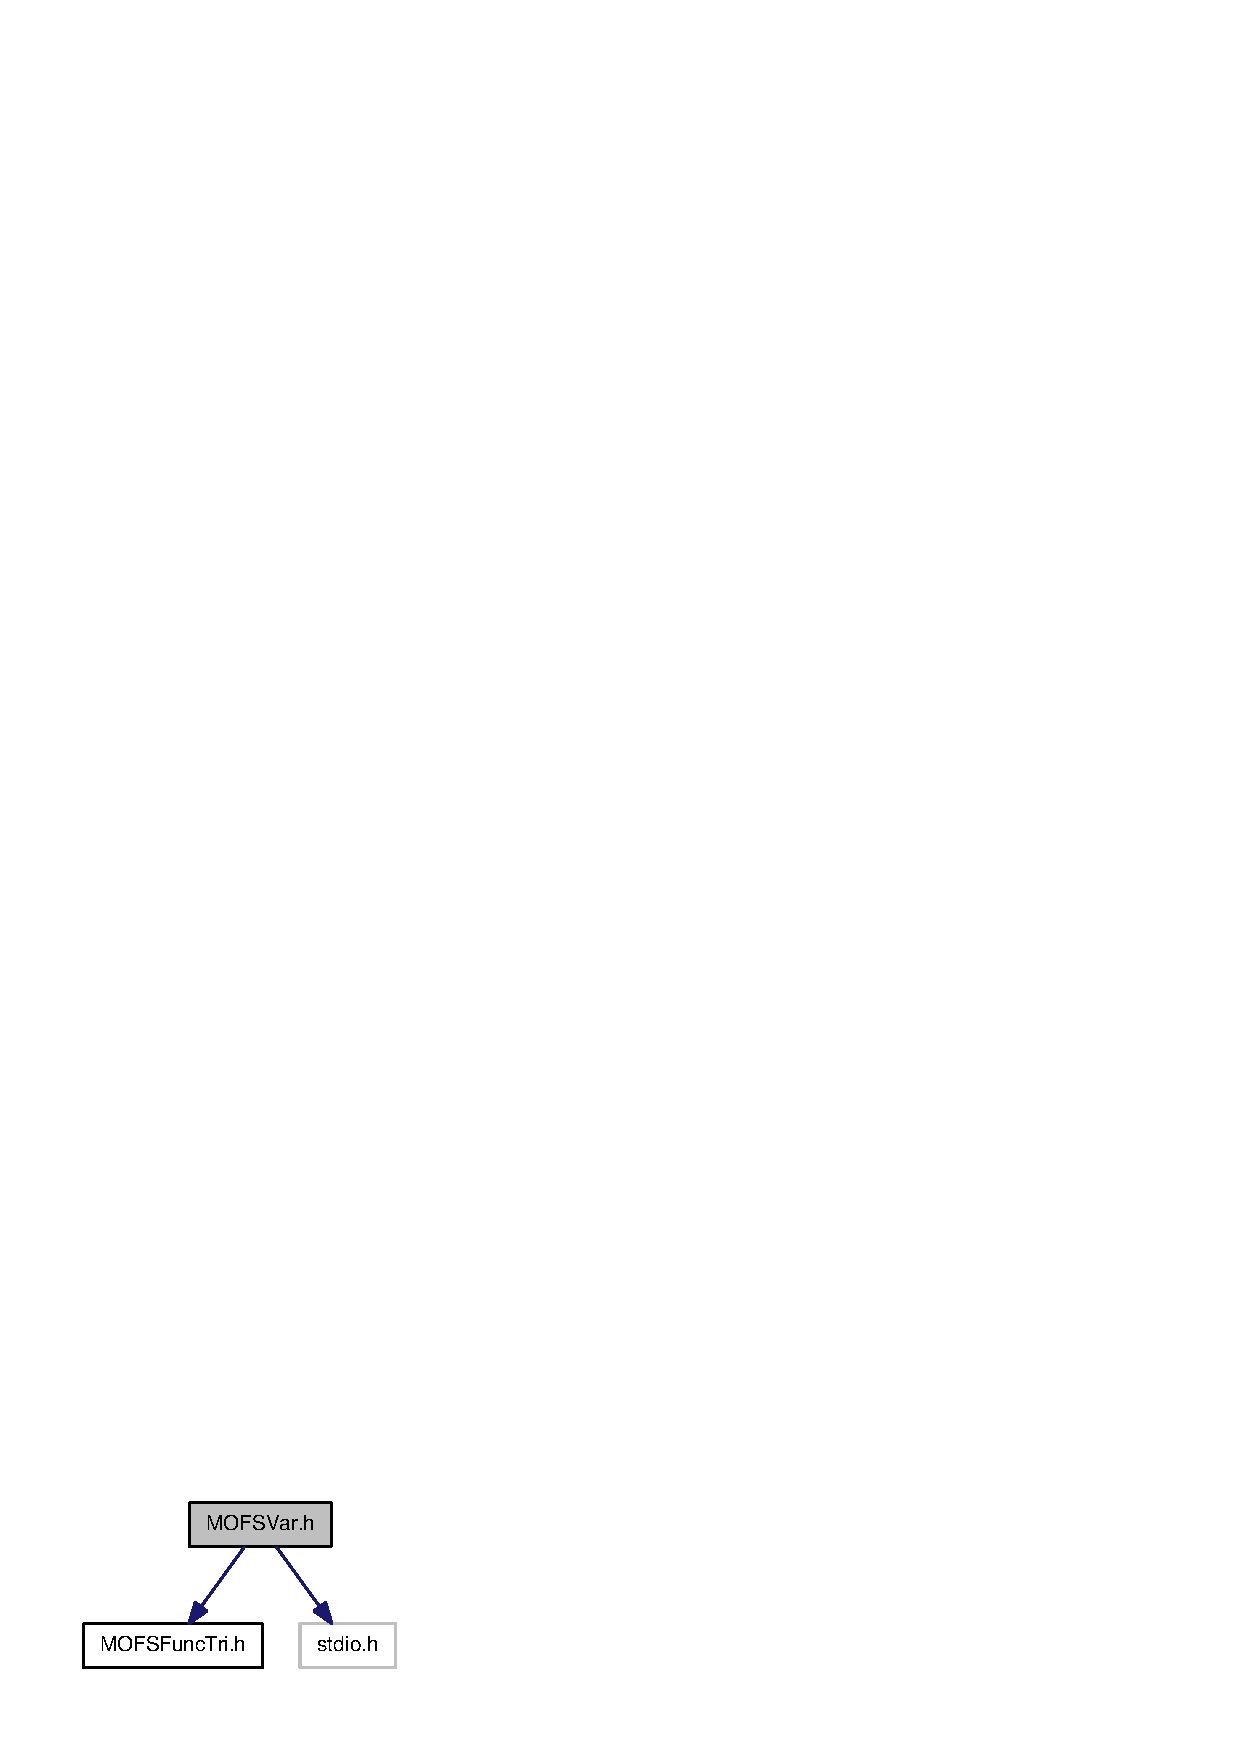
\includegraphics[width=194pt]{MOFSVar_8h__incl}
\end{center}
\end{figure}
This graph shows which files directly or indirectly include this file\-:\nopagebreak
\begin{figure}[H]
\begin{center}
\leavevmode
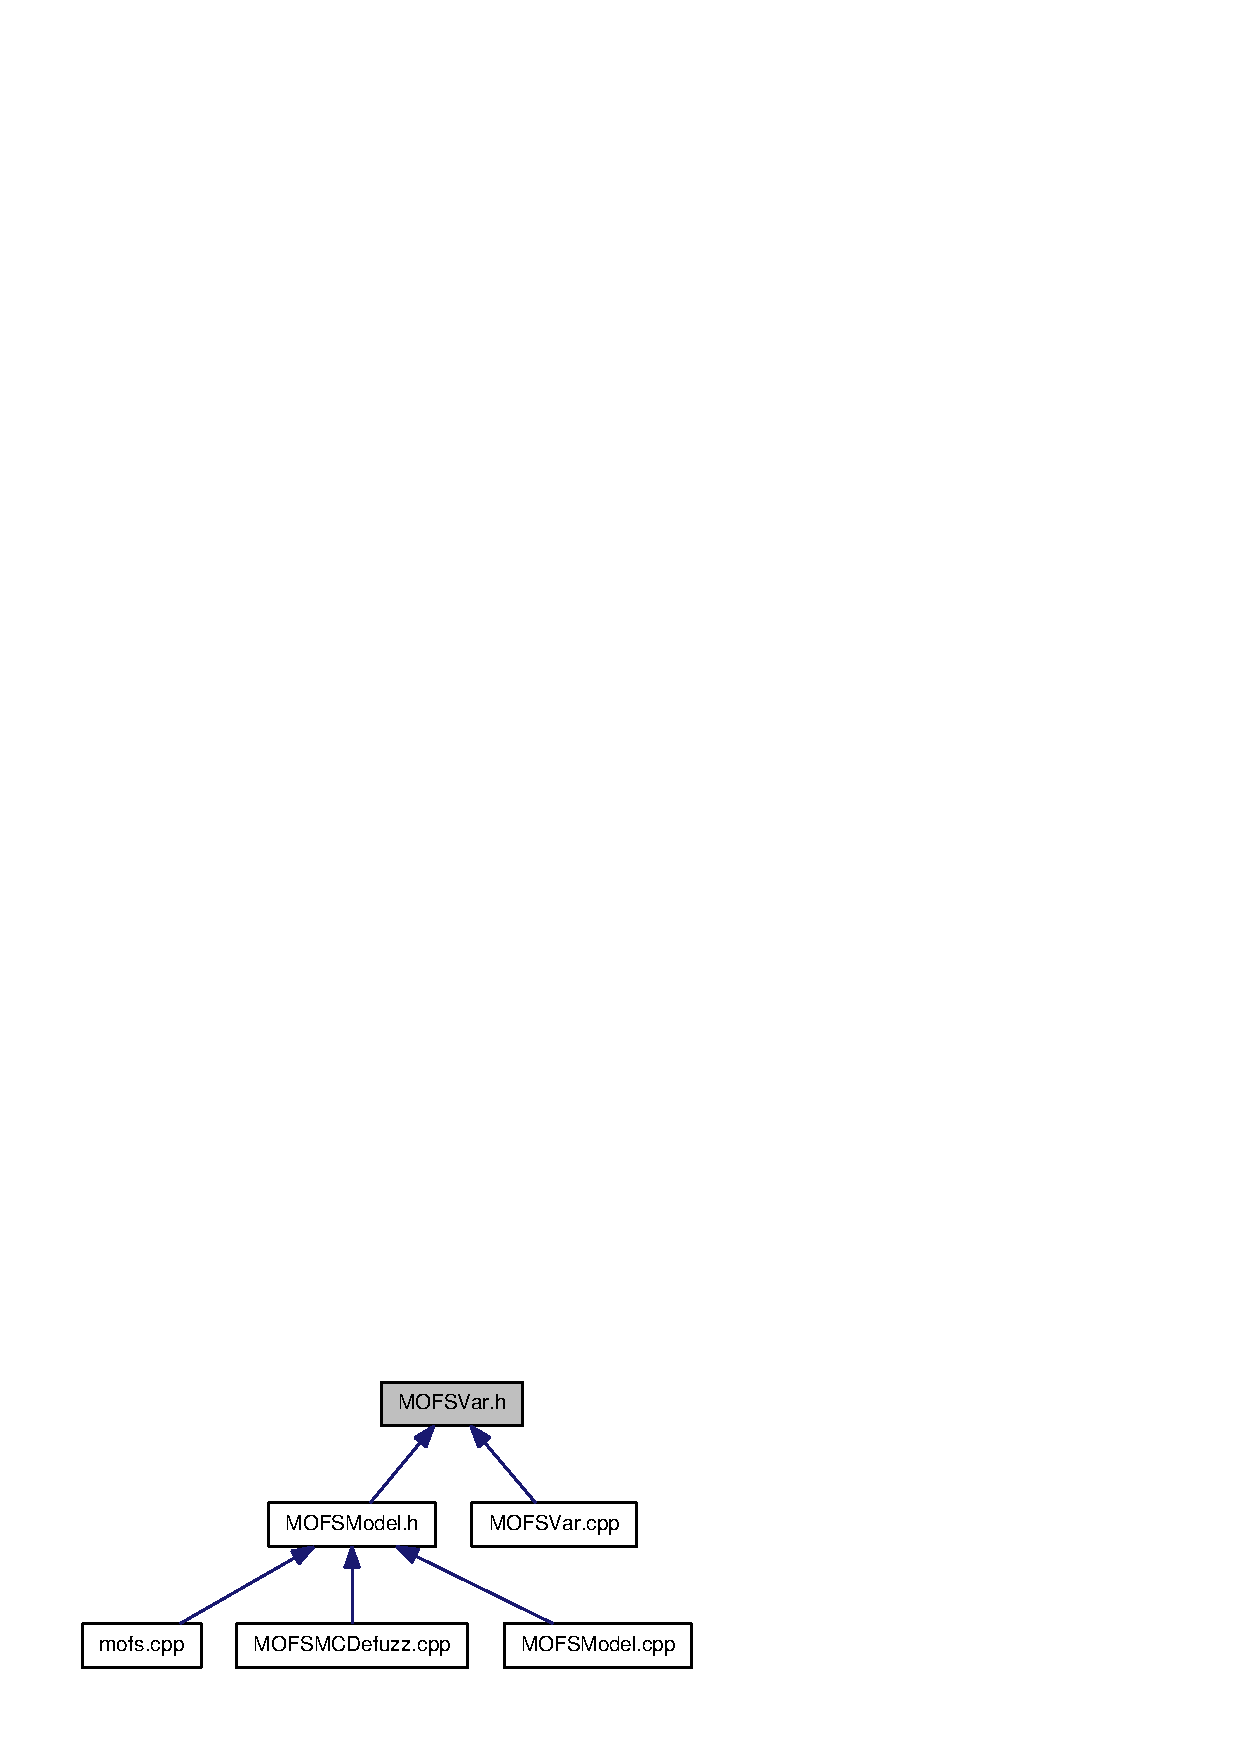
\includegraphics[width=336pt]{MOFSVar_8h__dep__incl}
\end{center}
\end{figure}
\subsection*{Classes}
\begin{DoxyCompactItemize}
\item 
class {\bf M\-O\-F\-S\-Var}
\item 
struct {\bf M\-O\-F\-S\-Var\-::\-Var\-Values}
\item 
struct {\bf M\-O\-F\-S\-Var\-::\-X\-Array}
\end{DoxyCompactItemize}

%--- End generated contents ---

% Index
\newpage
\phantomsection
\addcontentsline{toc}{chapter}{Index}
\printindex

\end{document}
